\documentclass[twoside]{book}

% Packages required by doxygen
\usepackage{fixltx2e}
\usepackage{calc}
\usepackage{doxygen}
\usepackage[export]{adjustbox} % also loads graphicx
\usepackage{graphicx}
\usepackage[utf8]{inputenc}
\usepackage{makeidx}
\usepackage{multicol}
\usepackage{multirow}
\PassOptionsToPackage{warn}{textcomp}
\usepackage{textcomp}
\usepackage[nointegrals]{wasysym}
\usepackage[table]{xcolor}

% Font selection
\usepackage[T1]{fontenc}
\usepackage[scaled=.90]{helvet}
\usepackage{courier}
\usepackage{amssymb}
\usepackage{sectsty}
\renewcommand{\familydefault}{\sfdefault}
\allsectionsfont{%
  \fontseries{bc}\selectfont%
  \color{darkgray}%
}
\renewcommand{\DoxyLabelFont}{%
  \fontseries{bc}\selectfont%
  \color{darkgray}%
}
\newcommand{\+}{\discretionary{\mbox{\scriptsize$\hookleftarrow$}}{}{}}

% Page & text layout
\usepackage{geometry}
\geometry{%
  a4paper,%
  top=2.5cm,%
  bottom=2.5cm,%
  left=2.5cm,%
  right=2.5cm%
}
\tolerance=750
\hfuzz=15pt
\hbadness=750
\setlength{\emergencystretch}{15pt}
\setlength{\parindent}{0cm}
\setlength{\parskip}{3ex plus 2ex minus 2ex}
\makeatletter
\renewcommand{\paragraph}{%
  \@startsection{paragraph}{4}{0ex}{-1.0ex}{1.0ex}{%
    \normalfont\normalsize\bfseries\SS@parafont%
  }%
}
\renewcommand{\subparagraph}{%
  \@startsection{subparagraph}{5}{0ex}{-1.0ex}{1.0ex}{%
    \normalfont\normalsize\bfseries\SS@subparafont%
  }%
}
\makeatother

% Headers & footers
\usepackage{fancyhdr}
\pagestyle{fancyplain}
\fancyhead[LE]{\fancyplain{}{\bfseries\thepage}}
\fancyhead[CE]{\fancyplain{}{}}
\fancyhead[RE]{\fancyplain{}{\bfseries\leftmark}}
\fancyhead[LO]{\fancyplain{}{\bfseries\rightmark}}
\fancyhead[CO]{\fancyplain{}{}}
\fancyhead[RO]{\fancyplain{}{\bfseries\thepage}}
\fancyfoot[LE]{\fancyplain{}{}}
\fancyfoot[CE]{\fancyplain{}{}}
\fancyfoot[RE]{\fancyplain{}{\bfseries\scriptsize Generated by Doxygen }}
\fancyfoot[LO]{\fancyplain{}{\bfseries\scriptsize Generated by Doxygen }}
\fancyfoot[CO]{\fancyplain{}{}}
\fancyfoot[RO]{\fancyplain{}{}}
\renewcommand{\footrulewidth}{0.4pt}
\renewcommand{\chaptermark}[1]{%
  \markboth{#1}{}%
}
\renewcommand{\sectionmark}[1]{%
  \markright{\thesection\ #1}%
}

% Indices & bibliography
\usepackage{natbib}
\usepackage[titles]{tocloft}
\setcounter{tocdepth}{3}
\setcounter{secnumdepth}{5}
\makeindex

% Hyperlinks (required, but should be loaded last)
\usepackage{ifpdf}
\ifpdf
  \usepackage[pdftex,pagebackref=true]{hyperref}
\else
  \usepackage[ps2pdf,pagebackref=true]{hyperref}
\fi
\hypersetup{%
  colorlinks=true,%
  linkcolor=blue,%
  citecolor=blue,%
  unicode%
}

% Custom commands
\newcommand{\clearemptydoublepage}{%
  \newpage{\pagestyle{empty}\cleardoublepage}%
}

\usepackage{caption}
\captionsetup{labelsep=space,justification=centering,font={bf},singlelinecheck=off,skip=4pt,position=top}

%===== C O N T E N T S =====

\begin{document}

% Titlepage & ToC
\hypersetup{pageanchor=false,
             bookmarksnumbered=true,
             pdfencoding=unicode
            }
\pagenumbering{alph}
\begin{titlepage}
\vspace*{7cm}
\begin{center}%
{\Large Game Library }\\
\vspace*{1cm}
{\large Generated by Doxygen 1.8.13}\\
\end{center}
\end{titlepage}
\clearemptydoublepage
\pagenumbering{roman}
\tableofcontents
\clearemptydoublepage
\pagenumbering{arabic}
\hypersetup{pageanchor=true}

%--- Begin generated contents ---
\chapter{Hierarchical Index}
\section{Class Hierarchy}
This inheritance list is sorted roughly, but not completely, alphabetically\+:\begin{DoxyCompactList}
\item \contentsline{section}{Banco}{\pageref{class_banco}}{}
\item \contentsline{section}{Biblioteca}{\pageref{class_biblioteca}}{}
\item \contentsline{section}{Cartao\+Credito}{\pageref{class_cartao_credito}}{}
\item \contentsline{section}{contactos}{\pageref{structcontactos}}{}
\item \contentsline{section}{Data}{\pageref{class_data}}{}
\item \contentsline{section}{Empresa}{\pageref{class_empresa}}{}
\item \contentsline{section}{Empresas\+Comp}{\pageref{struct_empresas_comp}}{}
\item \contentsline{section}{Erro}{\pageref{class_erro}}{}
\begin{DoxyCompactList}
\item \contentsline{section}{Cartao\+Inexistente}{\pageref{class_cartao_inexistente}}{}
\item \contentsline{section}{Cartao\+Invalido}{\pageref{class_cartao_invalido}}{}
\item \contentsline{section}{Cartao\+Ja\+Existente}{\pageref{class_cartao_ja_existente}}{}
\item \contentsline{section}{Data\+Invalida}{\pageref{class_data_invalida}}{}
\item \contentsline{section}{Empresa\+Inexistente}{\pageref{class_empresa_inexistente}}{}
\item \contentsline{section}{Empresa\+Ja\+Adicionada}{\pageref{class_empresa_ja_adicionada}}{}
\item \contentsline{section}{Erro\+Email}{\pageref{class_erro_email}}{}
\item \contentsline{section}{Input\+Invalido}{\pageref{class_input_invalido}}{}
\item \contentsline{section}{Plataforma\+Ja\+Existente}{\pageref{class_plataforma_ja_existente}}{}
\item \contentsline{section}{Plataforma\+Nao\+Existente}{\pageref{class_plataforma_nao_existente}}{}
\item \contentsline{section}{Preco\+Invalido}{\pageref{class_preco_invalido}}{}
\item \contentsline{section}{Saldo\+Insuficiente}{\pageref{class_saldo_insuficiente}}{}
\item \contentsline{section}{Titulo\+Inexistente}{\pageref{class_titulo_inexistente}}{}
\item \contentsline{section}{Titulo\+Ja\+Adicionado}{\pageref{class_titulo_ja_adicionado}}{}
\item \contentsline{section}{Utilizador\+Inexistente}{\pageref{class_utilizador_inexistente}}{}
\end{DoxyCompactList}
\item \contentsline{section}{Sistema}{\pageref{class_sistema}}{}
\item \contentsline{section}{Titulo}{\pageref{class_titulo}}{}
\begin{DoxyCompactList}
\item \contentsline{section}{Home}{\pageref{class_home}}{}
\item \contentsline{section}{Online}{\pageref{class_online}}{}
\end{DoxyCompactList}
\item \contentsline{section}{Utilizador}{\pageref{class_utilizador}}{}
\item \contentsline{section}{Utilizador\+Ptr}{\pageref{struct_utilizador_ptr}}{}
\item \contentsline{section}{Wished\+Title}{\pageref{class_wished_title}}{}
\end{DoxyCompactList}

\chapter{Class Index}
\section{Class List}
Here are the classes, structs, unions and interfaces with brief descriptions\+:\begin{DoxyCompactList}
\item\contentsline{section}{\hyperlink{classBanco}{Banco} }{\pageref{classBanco}}{}
\item\contentsline{section}{\hyperlink{classBiblioteca}{Biblioteca} }{\pageref{classBiblioteca}}{}
\item\contentsline{section}{\hyperlink{classCartaoCredito}{Cartao\+Credito} }{\pageref{classCartaoCredito}}{}
\item\contentsline{section}{\hyperlink{classCartaoInexistente}{Cartao\+Inexistente} }{\pageref{classCartaoInexistente}}{}
\item\contentsline{section}{\hyperlink{classCartaoInvalido}{Cartao\+Invalido} }{\pageref{classCartaoInvalido}}{}
\item\contentsline{section}{\hyperlink{classCartaoJaExistente}{Cartao\+Ja\+Existente} }{\pageref{classCartaoJaExistente}}{}
\item\contentsline{section}{\hyperlink{structcontactos}{contactos} }{\pageref{structcontactos}}{}
\item\contentsline{section}{\hyperlink{classData}{Data} }{\pageref{classData}}{}
\item\contentsline{section}{\hyperlink{classDataInvalida}{Data\+Invalida} }{\pageref{classDataInvalida}}{}
\item\contentsline{section}{\hyperlink{classEmpresa}{Empresa} }{\pageref{classEmpresa}}{}
\item\contentsline{section}{\hyperlink{classEmpresaInexistente}{Empresa\+Inexistente} }{\pageref{classEmpresaInexistente}}{}
\item\contentsline{section}{\hyperlink{classEmpresaJaAdicionada}{Empresa\+Ja\+Adicionada} }{\pageref{classEmpresaJaAdicionada}}{}
\item\contentsline{section}{\hyperlink{structEmpresasComp}{Empresas\+Comp} }{\pageref{structEmpresasComp}}{}
\item\contentsline{section}{\hyperlink{classErro}{Erro} }{\pageref{classErro}}{}
\item\contentsline{section}{\hyperlink{classErroEmail}{Erro\+Email} }{\pageref{classErroEmail}}{}
\item\contentsline{section}{\hyperlink{classHome}{Home} }{\pageref{classHome}}{}
\item\contentsline{section}{\hyperlink{classInputInvalido}{Input\+Invalido} }{\pageref{classInputInvalido}}{}
\item\contentsline{section}{\hyperlink{classOnline}{Online} }{\pageref{classOnline}}{}
\item\contentsline{section}{\hyperlink{classPlataformaJaExistente}{Plataforma\+Ja\+Existente} }{\pageref{classPlataformaJaExistente}}{}
\item\contentsline{section}{\hyperlink{classPlataformaNaoExistente}{Plataforma\+Nao\+Existente} }{\pageref{classPlataformaNaoExistente}}{}
\item\contentsline{section}{\hyperlink{classPrecoInvalido}{Preco\+Invalido} }{\pageref{classPrecoInvalido}}{}
\item\contentsline{section}{\hyperlink{classSaldoInsuficiente}{Saldo\+Insuficiente} }{\pageref{classSaldoInsuficiente}}{}
\item\contentsline{section}{\hyperlink{classSistema}{Sistema} }{\pageref{classSistema}}{}
\item\contentsline{section}{\hyperlink{classTitulo}{Titulo} }{\pageref{classTitulo}}{}
\item\contentsline{section}{\hyperlink{classTituloInexistente}{Titulo\+Inexistente} }{\pageref{classTituloInexistente}}{}
\item\contentsline{section}{\hyperlink{classTituloJaAdicionado}{Titulo\+Ja\+Adicionado} }{\pageref{classTituloJaAdicionado}}{}
\item\contentsline{section}{\hyperlink{classUtilizador}{Utilizador} }{\pageref{classUtilizador}}{}
\item\contentsline{section}{\hyperlink{classUtilizadorInexistente}{Utilizador\+Inexistente} }{\pageref{classUtilizadorInexistente}}{}
\item\contentsline{section}{\hyperlink{structUtilizadorPtr}{Utilizador\+Ptr} }{\pageref{structUtilizadorPtr}}{}
\item\contentsline{section}{\hyperlink{classWishedTitle}{Wished\+Title} }{\pageref{classWishedTitle}}{}
\end{DoxyCompactList}

\chapter{File Index}
\section{File List}
Here is a list of all files with brief descriptions\+:\begin{DoxyCompactList}
\item\contentsline{section}{\mbox{\hyperlink{_banco_8cpp}{Banco.\+cpp}} }{\pageref{_banco_8cpp}}{}
\item\contentsline{section}{\mbox{\hyperlink{_banco_8h}{Banco.\+h}} }{\pageref{_banco_8h}}{}
\item\contentsline{section}{\mbox{\hyperlink{_biblioteca_8cpp}{Biblioteca.\+cpp}} }{\pageref{_biblioteca_8cpp}}{}
\item\contentsline{section}{\mbox{\hyperlink{_biblioteca_8h}{Biblioteca.\+h}} }{\pageref{_biblioteca_8h}}{}
\item\contentsline{section}{\mbox{\hyperlink{_cartao_credito_8cpp}{Cartao\+Credito.\+cpp}} }{\pageref{_cartao_credito_8cpp}}{}
\item\contentsline{section}{\mbox{\hyperlink{_cartao_credito_8h}{Cartao\+Credito.\+h}} }{\pageref{_cartao_credito_8h}}{}
\item\contentsline{section}{\mbox{\hyperlink{_data_8cpp}{Data.\+cpp}} }{\pageref{_data_8cpp}}{}
\item\contentsline{section}{\mbox{\hyperlink{_data_8h}{Data.\+h}} }{\pageref{_data_8h}}{}
\item\contentsline{section}{\mbox{\hyperlink{_empresa_8cpp}{Empresa.\+cpp}} }{\pageref{_empresa_8cpp}}{}
\item\contentsline{section}{\mbox{\hyperlink{_empresa_8h}{Empresa.\+h}} }{\pageref{_empresa_8h}}{}
\item\contentsline{section}{\mbox{\hyperlink{_erro_8h}{Erro.\+h}} }{\pageref{_erro_8h}}{}
\item\contentsline{section}{\mbox{\hyperlink{main_8cpp}{main.\+cpp}} }{\pageref{main_8cpp}}{}
\item\contentsline{section}{\mbox{\hyperlink{_sistema_8cpp}{Sistema.\+cpp}} }{\pageref{_sistema_8cpp}}{}
\item\contentsline{section}{\mbox{\hyperlink{_sistema_8h}{Sistema.\+h}} }{\pageref{_sistema_8h}}{}
\item\contentsline{section}{\mbox{\hyperlink{_titulo_8cpp}{Titulo.\+cpp}} }{\pageref{_titulo_8cpp}}{}
\item\contentsline{section}{\mbox{\hyperlink{_titulo_8h}{Titulo.\+h}} }{\pageref{_titulo_8h}}{}
\item\contentsline{section}{\mbox{\hyperlink{_utilizador_8cpp}{Utilizador.\+cpp}} }{\pageref{_utilizador_8cpp}}{}
\item\contentsline{section}{\mbox{\hyperlink{_utilizador_8h}{Utilizador.\+h}} }{\pageref{_utilizador_8h}}{}
\item\contentsline{section}{\mbox{\hyperlink{_wished_title_8cpp}{Wished\+Title.\+cpp}} }{\pageref{_wished_title_8cpp}}{}
\item\contentsline{section}{\mbox{\hyperlink{_wished_title_8h}{Wished\+Title.\+h}} }{\pageref{_wished_title_8h}}{}
\end{DoxyCompactList}

\chapter{Class Documentation}
\hypertarget{classBanco}{}\section{Banco Class Reference}
\label{classBanco}\index{Banco@{Banco}}


{\ttfamily \#include $<$Banco.\+h$>$}

\subsection*{Public Member Functions}
\begin{DoxyCompactItemize}
\item 
\hyperlink{classBanco_a686e51b219dc175e432e91559298b259}{Banco} ()
\begin{DoxyCompactList}\small\item\em Construtor da classe \hyperlink{classBanco}{Banco}. \end{DoxyCompactList}\item 
\hyperlink{classBanco_af69f9b0da3521d7c1e422f21dfd5829e}{$\sim$\+Banco} ()
\begin{DoxyCompactList}\small\item\em Destrutor da class \hyperlink{classBanco}{Banco}. \end{DoxyCompactList}\item 
void \hyperlink{classBanco_a227af53b49995242c06d89bb10ffc8ea}{set\+Data\+Atual} ()
\begin{DoxyCompactList}\small\item\em atualiza a data, para a data atual \end{DoxyCompactList}\item 
\hyperlink{classData}{Data} \hyperlink{classBanco_a0735f07636c578666068a16f6ecccd91}{get\+Data\+Atual} () const
\begin{DoxyCompactList}\small\item\em Devolve a data atual. \end{DoxyCompactList}\item 
std\+::vector$<$ \hyperlink{classCartaoCredito}{Cartao\+Credito} $>$ \hyperlink{classBanco_a859463228f6bf63d32d70afe8efd9541}{get\+Cartoes\+Credito} () const
\begin{DoxyCompactList}\small\item\em Permite obter os cartoes de credito dos utilizadores. \end{DoxyCompactList}\item 
bool \hyperlink{classBanco_ac469cc9db5980081701bf9eb27a7e612}{is\+Data\+Valida} (const \hyperlink{classCartaoCredito}{Cartao\+Credito} \&cartao) const
\begin{DoxyCompactList}\small\item\em Verifica se uma data e valida. \end{DoxyCompactList}\item 
void \hyperlink{classBanco_a2ac1bb3c6a742743bcbb6dd0a312d74d}{adiciona\+Cartao\+Credito} (const \hyperlink{classCartaoCredito}{Cartao\+Credito} \&cartao)
\begin{DoxyCompactList}\small\item\em Adiciona um cartao de credito ao banco. \end{DoxyCompactList}\item 
void \hyperlink{classBanco_a5f36ab07909fc570d158a21e2e6398f5}{adiciona\+Cartoes\+Credito} (const std\+::vector$<$ \hyperlink{classCartaoCredito}{Cartao\+Credito} $>$ \&cartoes)
\begin{DoxyCompactList}\small\item\em Adiciona um vector de cartoes de credito ao banco. \end{DoxyCompactList}\item 
void \hyperlink{classBanco_a8c8f743903ba86129b62afbb3813e6f0}{atualiza\+Cartao} (\hyperlink{classCartaoCredito}{Cartao\+Credito} \&cartao)
\begin{DoxyCompactList}\small\item\em Atualiza a data de um cartao de credito, adicionando mais 3 anos de validade, se esta fora da validade ou se faltam ate 90 dias ate ao fim do prazo. \end{DoxyCompactList}\item 
void \hyperlink{classBanco_ad6f39d091c83361878bc5cfda534a49d}{atualiza\+Cartoes\+Credito} ()
\begin{DoxyCompactList}\small\item\em Atualiza todos os cartoes do sistema. \end{DoxyCompactList}\end{DoxyCompactItemize}


\subsection{Detailed Description}
\hyperlink{classBanco}{Banco} que contem os cartoes de credito dos utilizadores. 

\subsection{Constructor \& Destructor Documentation}
\mbox{\Hypertarget{classBanco_a686e51b219dc175e432e91559298b259}\label{classBanco_a686e51b219dc175e432e91559298b259}} 
\index{Banco@{Banco}!Banco@{Banco}}
\index{Banco@{Banco}!Banco@{Banco}}
\subsubsection{\texorpdfstring{Banco()}{Banco()}}
{\footnotesize\ttfamily Banco\+::\+Banco (\begin{DoxyParamCaption}{ }\end{DoxyParamCaption})}



Construtor da classe \hyperlink{classBanco}{Banco}. 


\begin{DoxyCode}
10              \{
11     time\_t theTime = time(NULL);
12     \textcolor{keyword}{struct }tm *aTime = localtime(&theTime);
13 
14     \textcolor{keywordtype}{unsigned} \textcolor{keywordtype}{int} dia= aTime->tm\_mday;
15     \textcolor{keywordtype}{unsigned} \textcolor{keywordtype}{int} mes = aTime->tm\_mon + 1; \textcolor{comment}{// Month is 0 - 11, add 1 to get a jan-dec 1-12 concept}
16     \textcolor{keywordtype}{unsigned} \textcolor{keywordtype}{int} ano = aTime->tm\_year + 1900;
17 
18     this->atual.\hyperlink{classData_a3e2c5356bc8d548b75c7d085f7a7c4ee}{setDia}(dia).\hyperlink{classData_ab15051ae481d89d057b22abc8152584c}{setMes}(mes).\hyperlink{classData_a8d4cfad647b590df436d8260000a2745}{setAno}(ano);
19 \}
\end{DoxyCode}
Here is the call graph for this function\+:
\nopagebreak
\begin{figure}[H]
\begin{center}
\leavevmode
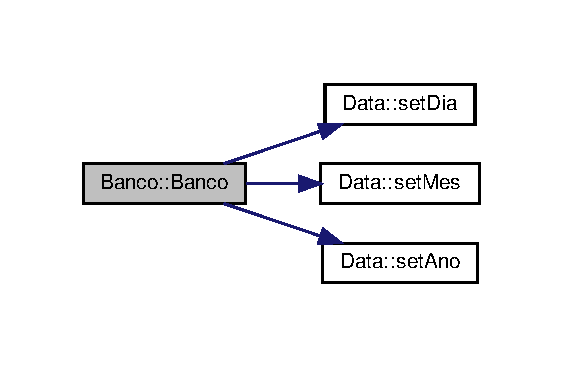
\includegraphics[width=270pt]{classBanco_a686e51b219dc175e432e91559298b259_cgraph}
\end{center}
\end{figure}
\mbox{\Hypertarget{classBanco_af69f9b0da3521d7c1e422f21dfd5829e}\label{classBanco_af69f9b0da3521d7c1e422f21dfd5829e}} 
\index{Banco@{Banco}!````~Banco@{$\sim$\+Banco}}
\index{````~Banco@{$\sim$\+Banco}!Banco@{Banco}}
\subsubsection{\texorpdfstring{$\sim$\+Banco()}{~Banco()}}
{\footnotesize\ttfamily Banco\+::$\sim$\+Banco (\begin{DoxyParamCaption}{ }\end{DoxyParamCaption})}



Destrutor da class \hyperlink{classBanco}{Banco}. 


\begin{DoxyCode}
21               \{
22 
23 \}
\end{DoxyCode}


\subsection{Member Function Documentation}
\mbox{\Hypertarget{classBanco_a2ac1bb3c6a742743bcbb6dd0a312d74d}\label{classBanco_a2ac1bb3c6a742743bcbb6dd0a312d74d}} 
\index{Banco@{Banco}!adiciona\+Cartao\+Credito@{adiciona\+Cartao\+Credito}}
\index{adiciona\+Cartao\+Credito@{adiciona\+Cartao\+Credito}!Banco@{Banco}}
\subsubsection{\texorpdfstring{adiciona\+Cartao\+Credito()}{adicionaCartaoCredito()}}
{\footnotesize\ttfamily void Banco\+::adiciona\+Cartao\+Credito (\begin{DoxyParamCaption}\item[{const \hyperlink{classCartaoCredito}{Cartao\+Credito} \&}]{cartao }\end{DoxyParamCaption})}



Adiciona um cartao de credito ao banco. 


\begin{DoxyParams}{Parameters}
{\em cartao} & -\/ cartao de credito a adicionar \\
\hline
\end{DoxyParams}

\begin{DoxyCode}
46 \{
47     \textcolor{comment}{/*ve se ja existe cartao de credito*/}
48     \textcolor{keywordflow}{if} (find(this->CartoesDeCredito.begin(),this->CartoesDeCredito.end(),C) != this->CartoesDeCredito.end()
      )
49         \textcolor{keywordflow}{throw} \hyperlink{classCartaoJaExistente}{CartaoJaExistente}(C.getId());
50 
51     this->CartoesDeCredito.push\_back(C);
52 \}
\end{DoxyCode}
Here is the call graph for this function\+:
\nopagebreak
\begin{figure}[H]
\begin{center}
\leavevmode
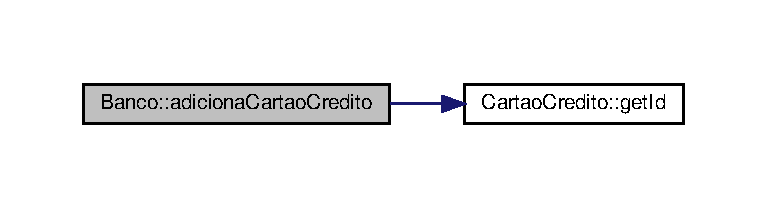
\includegraphics[width=350pt]{classBanco_a2ac1bb3c6a742743bcbb6dd0a312d74d_cgraph}
\end{center}
\end{figure}
Here is the caller graph for this function\+:
\nopagebreak
\begin{figure}[H]
\begin{center}
\leavevmode
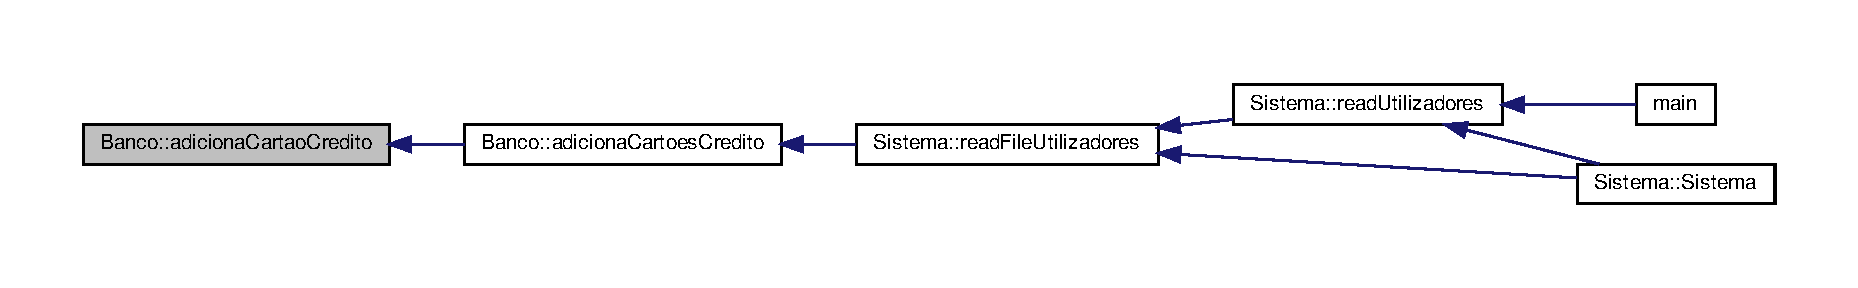
\includegraphics[width=350pt]{classBanco_a2ac1bb3c6a742743bcbb6dd0a312d74d_icgraph}
\end{center}
\end{figure}
\mbox{\Hypertarget{classBanco_a5f36ab07909fc570d158a21e2e6398f5}\label{classBanco_a5f36ab07909fc570d158a21e2e6398f5}} 
\index{Banco@{Banco}!adiciona\+Cartoes\+Credito@{adiciona\+Cartoes\+Credito}}
\index{adiciona\+Cartoes\+Credito@{adiciona\+Cartoes\+Credito}!Banco@{Banco}}
\subsubsection{\texorpdfstring{adiciona\+Cartoes\+Credito()}{adicionaCartoesCredito()}}
{\footnotesize\ttfamily void Banco\+::adiciona\+Cartoes\+Credito (\begin{DoxyParamCaption}\item[{const std\+::vector$<$ \hyperlink{classCartaoCredito}{Cartao\+Credito} $>$ \&}]{cartoes }\end{DoxyParamCaption})}



Adiciona um vector de cartoes de credito ao banco. 


\begin{DoxyParams}{Parameters}
{\em cartoes} & -\/ vector de cartoes de credito a adicionar ao banco \\
\hline
\end{DoxyParams}

\begin{DoxyCode}
55 \{
56     \textcolor{keywordflow}{for} (\textcolor{keyword}{auto} \textcolor{keyword}{const} & cartao : cartoes)
57     \{
58         \hyperlink{classBanco_a2ac1bb3c6a742743bcbb6dd0a312d74d}{adicionaCartaoCredito}(cartao);
59     \}
60 \}
\end{DoxyCode}
Here is the call graph for this function\+:
\nopagebreak
\begin{figure}[H]
\begin{center}
\leavevmode
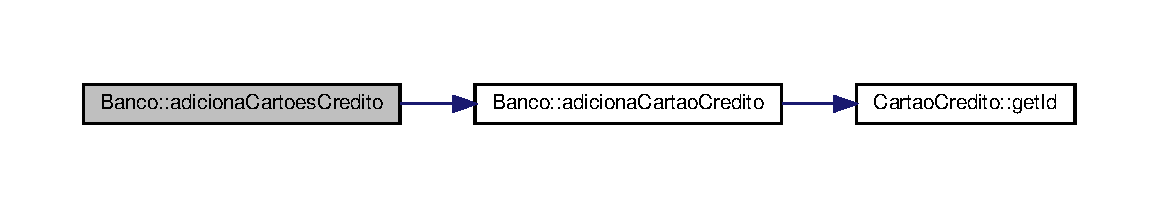
\includegraphics[width=350pt]{classBanco_a5f36ab07909fc570d158a21e2e6398f5_cgraph}
\end{center}
\end{figure}
Here is the caller graph for this function\+:
\nopagebreak
\begin{figure}[H]
\begin{center}
\leavevmode
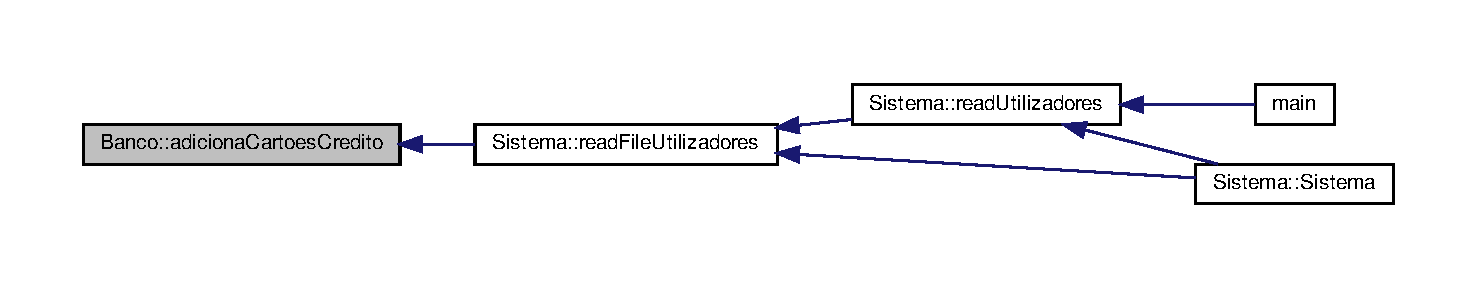
\includegraphics[width=350pt]{classBanco_a5f36ab07909fc570d158a21e2e6398f5_icgraph}
\end{center}
\end{figure}
\mbox{\Hypertarget{classBanco_a8c8f743903ba86129b62afbb3813e6f0}\label{classBanco_a8c8f743903ba86129b62afbb3813e6f0}} 
\index{Banco@{Banco}!atualiza\+Cartao@{atualiza\+Cartao}}
\index{atualiza\+Cartao@{atualiza\+Cartao}!Banco@{Banco}}
\subsubsection{\texorpdfstring{atualiza\+Cartao()}{atualizaCartao()}}
{\footnotesize\ttfamily void Banco\+::atualiza\+Cartao (\begin{DoxyParamCaption}\item[{\hyperlink{classCartaoCredito}{Cartao\+Credito} \&}]{cartao }\end{DoxyParamCaption})}



Atualiza a data de um cartao de credito, adicionando mais 3 anos de validade, se esta fora da validade ou se faltam ate 90 dias ate ao fim do prazo. 


\begin{DoxyParams}{Parameters}
{\em cartao} & -\/ cartao de credito a atualizar \\
\hline
\end{DoxyParams}

\begin{DoxyCode}
63 \{
64     \textcolor{keywordflow}{if}(!\hyperlink{classBanco_ac469cc9db5980081701bf9eb27a7e612}{isDataValida}(C))
65         C.atualizaDataDeValidade();
66     \textcolor{keywordflow}{else}
67     \{
68         \textcolor{keywordflow}{if} (C.getDataDeValidade().diferencaEntreDatas(this->\hyperlink{classBanco_a0735f07636c578666068a16f6ecccd91}{getDataAtual}()) <= 90)
69             C.atualizaDataDeValidade();
70     \}
71 \}
\end{DoxyCode}
Here is the call graph for this function\+:
\nopagebreak
\begin{figure}[H]
\begin{center}
\leavevmode
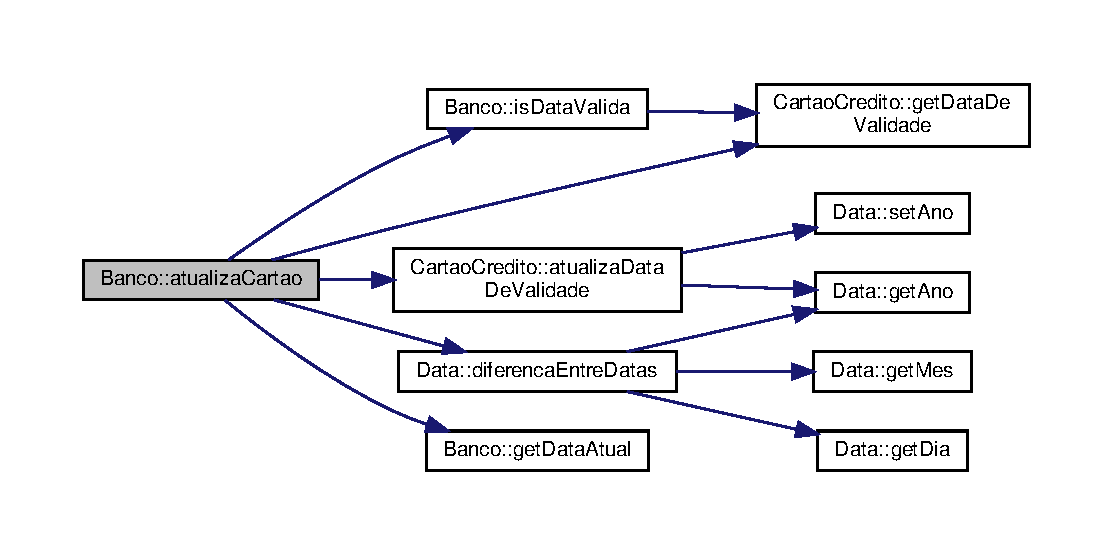
\includegraphics[width=350pt]{classBanco_a8c8f743903ba86129b62afbb3813e6f0_cgraph}
\end{center}
\end{figure}
Here is the caller graph for this function\+:
\nopagebreak
\begin{figure}[H]
\begin{center}
\leavevmode
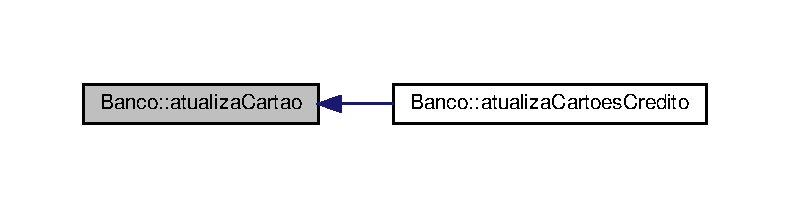
\includegraphics[width=350pt]{classBanco_a8c8f743903ba86129b62afbb3813e6f0_icgraph}
\end{center}
\end{figure}
\mbox{\Hypertarget{classBanco_ad6f39d091c83361878bc5cfda534a49d}\label{classBanco_ad6f39d091c83361878bc5cfda534a49d}} 
\index{Banco@{Banco}!atualiza\+Cartoes\+Credito@{atualiza\+Cartoes\+Credito}}
\index{atualiza\+Cartoes\+Credito@{atualiza\+Cartoes\+Credito}!Banco@{Banco}}
\subsubsection{\texorpdfstring{atualiza\+Cartoes\+Credito()}{atualizaCartoesCredito()}}
{\footnotesize\ttfamily void Banco\+::atualiza\+Cartoes\+Credito (\begin{DoxyParamCaption}{ }\end{DoxyParamCaption})}



Atualiza todos os cartoes do sistema. 


\begin{DoxyCode}
74 \{
75     \textcolor{keywordflow}{for}(\textcolor{keyword}{auto} & cartao : this->CartoesDeCredito)
76     \{
77         \hyperlink{classBanco_a8c8f743903ba86129b62afbb3813e6f0}{atualizaCartao}(cartao);
78     \}
79 \}
\end{DoxyCode}
Here is the call graph for this function\+:
\nopagebreak
\begin{figure}[H]
\begin{center}
\leavevmode
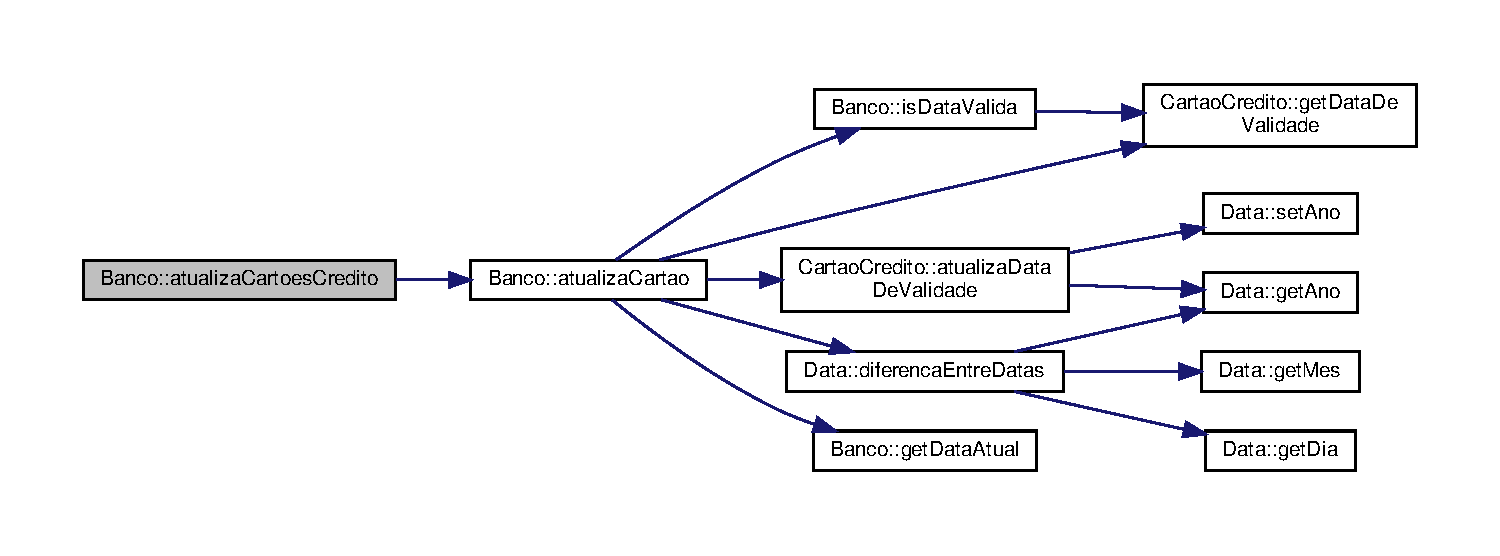
\includegraphics[width=350pt]{classBanco_ad6f39d091c83361878bc5cfda534a49d_cgraph}
\end{center}
\end{figure}
\mbox{\Hypertarget{classBanco_a859463228f6bf63d32d70afe8efd9541}\label{classBanco_a859463228f6bf63d32d70afe8efd9541}} 
\index{Banco@{Banco}!get\+Cartoes\+Credito@{get\+Cartoes\+Credito}}
\index{get\+Cartoes\+Credito@{get\+Cartoes\+Credito}!Banco@{Banco}}
\subsubsection{\texorpdfstring{get\+Cartoes\+Credito()}{getCartoesCredito()}}
{\footnotesize\ttfamily std\+::vector$<$ \hyperlink{classCartaoCredito}{Cartao\+Credito} $>$ Banco\+::get\+Cartoes\+Credito (\begin{DoxyParamCaption}{ }\end{DoxyParamCaption}) const}



Permite obter os cartoes de credito dos utilizadores. 

\begin{DoxyReturn}{Returns}
Retorna o vetor de cartoes de credito 
\end{DoxyReturn}

\begin{DoxyCode}
32 \{
33     \textcolor{keywordflow}{return} this->CartoesDeCredito;
34 \}
\end{DoxyCode}
Here is the caller graph for this function\+:
\nopagebreak
\begin{figure}[H]
\begin{center}
\leavevmode
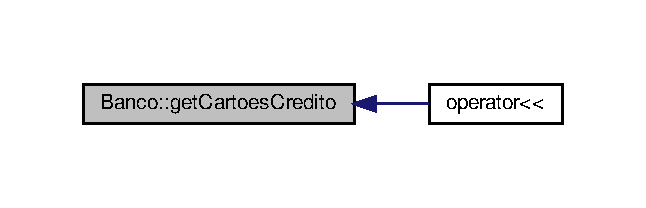
\includegraphics[width=310pt]{classBanco_a859463228f6bf63d32d70afe8efd9541_icgraph}
\end{center}
\end{figure}
\mbox{\Hypertarget{classBanco_a0735f07636c578666068a16f6ecccd91}\label{classBanco_a0735f07636c578666068a16f6ecccd91}} 
\index{Banco@{Banco}!get\+Data\+Atual@{get\+Data\+Atual}}
\index{get\+Data\+Atual@{get\+Data\+Atual}!Banco@{Banco}}
\subsubsection{\texorpdfstring{get\+Data\+Atual()}{getDataAtual()}}
{\footnotesize\ttfamily \hyperlink{classData}{Data} Banco\+::get\+Data\+Atual (\begin{DoxyParamCaption}{ }\end{DoxyParamCaption}) const}



Devolve a data atual. 

\begin{DoxyReturn}{Returns}
Retorna a data atual 
\end{DoxyReturn}

\begin{DoxyCode}
27 \{
28     \textcolor{keywordflow}{return} this->atual;
29 \}
\end{DoxyCode}
Here is the caller graph for this function\+:
\nopagebreak
\begin{figure}[H]
\begin{center}
\leavevmode
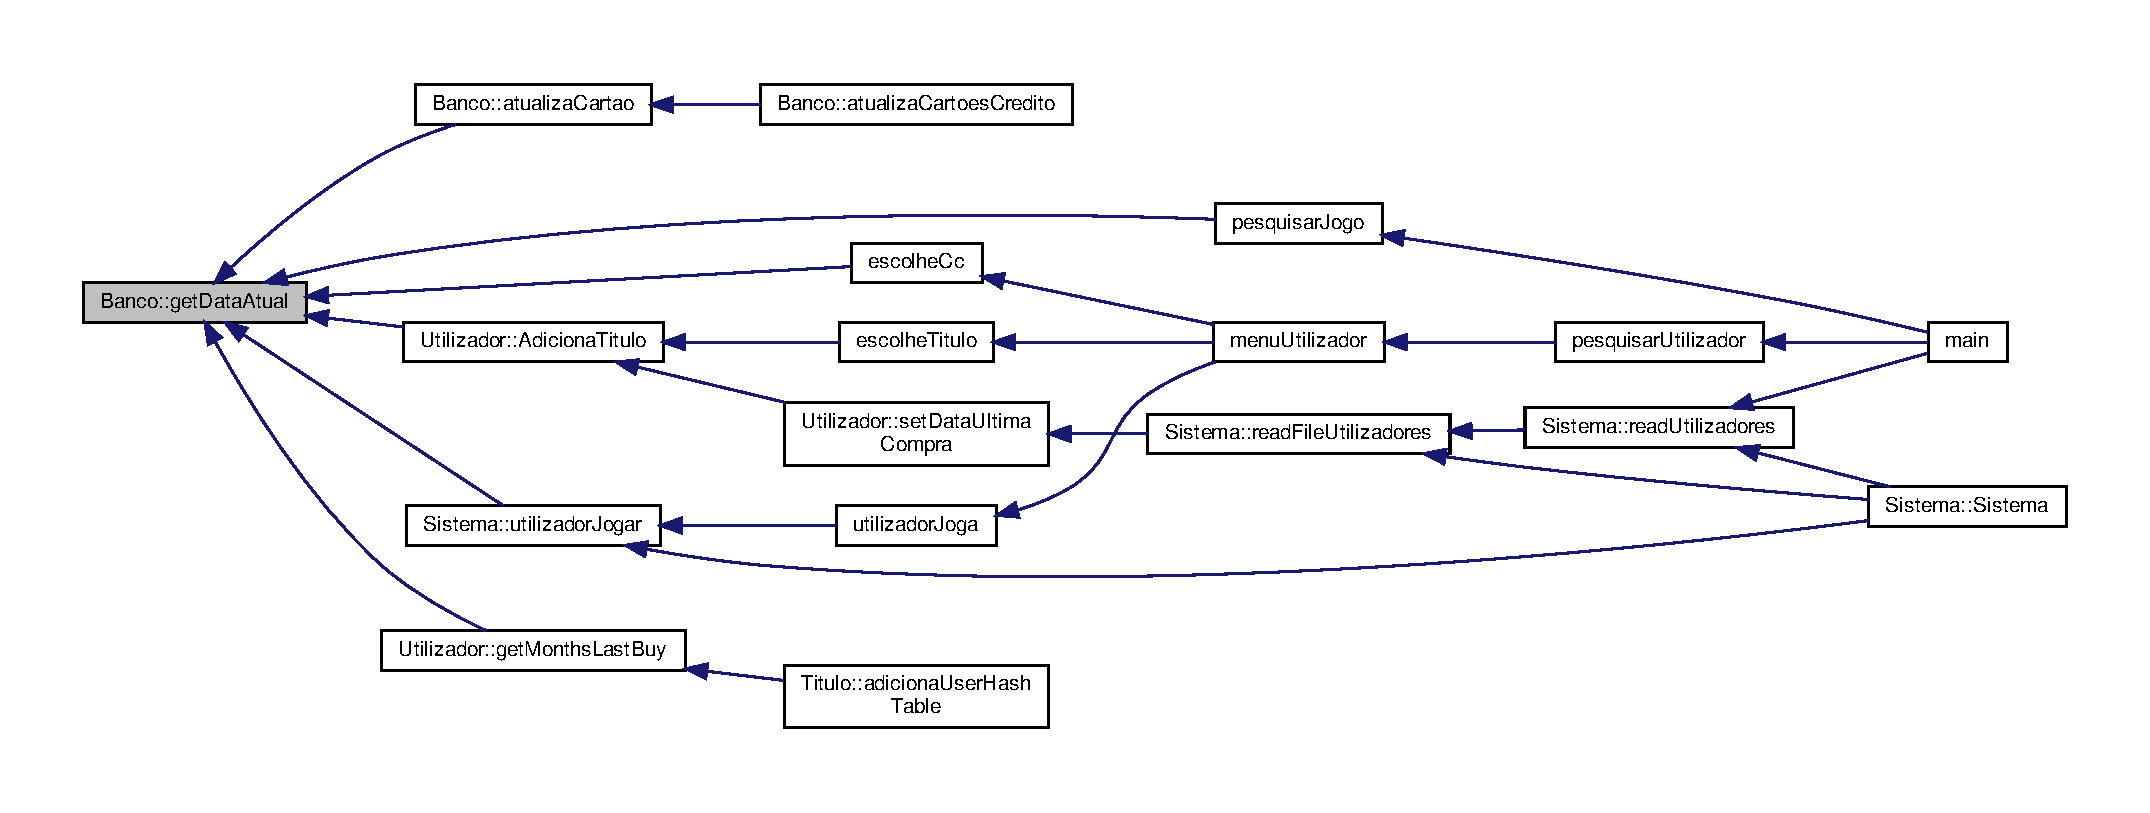
\includegraphics[width=350pt]{classBanco_a0735f07636c578666068a16f6ecccd91_icgraph}
\end{center}
\end{figure}
\mbox{\Hypertarget{classBanco_ac469cc9db5980081701bf9eb27a7e612}\label{classBanco_ac469cc9db5980081701bf9eb27a7e612}} 
\index{Banco@{Banco}!is\+Data\+Valida@{is\+Data\+Valida}}
\index{is\+Data\+Valida@{is\+Data\+Valida}!Banco@{Banco}}
\subsubsection{\texorpdfstring{is\+Data\+Valida()}{isDataValida()}}
{\footnotesize\ttfamily bool Banco\+::is\+Data\+Valida (\begin{DoxyParamCaption}\item[{const \hyperlink{classCartaoCredito}{Cartao\+Credito} \&}]{cartao }\end{DoxyParamCaption}) const}



Verifica se uma data e valida. 


\begin{DoxyParams}{Parameters}
{\em cartao} & -\/ cartao de credito cuja data vai ser verificada \\
\hline
\end{DoxyParams}
\begin{DoxyReturn}{Returns}
retorna true se a data for valida, ou false de outra forma 
\end{DoxyReturn}

\begin{DoxyCode}
37 \{
38         \textcolor{keywordflow}{if} (atual <= C.getDataDeValidade())
39             \textcolor{keywordflow}{return} \textcolor{keyword}{true};
40         \textcolor{keywordflow}{else}
41             \textcolor{keywordflow}{return} \textcolor{keyword}{false};
42 \}
\end{DoxyCode}
Here is the call graph for this function\+:
\nopagebreak
\begin{figure}[H]
\begin{center}
\leavevmode
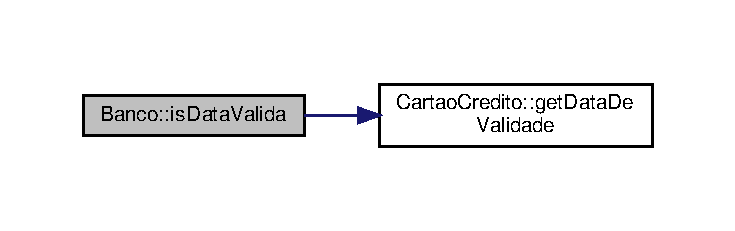
\includegraphics[width=350pt]{classBanco_ac469cc9db5980081701bf9eb27a7e612_cgraph}
\end{center}
\end{figure}
Here is the caller graph for this function\+:
\nopagebreak
\begin{figure}[H]
\begin{center}
\leavevmode
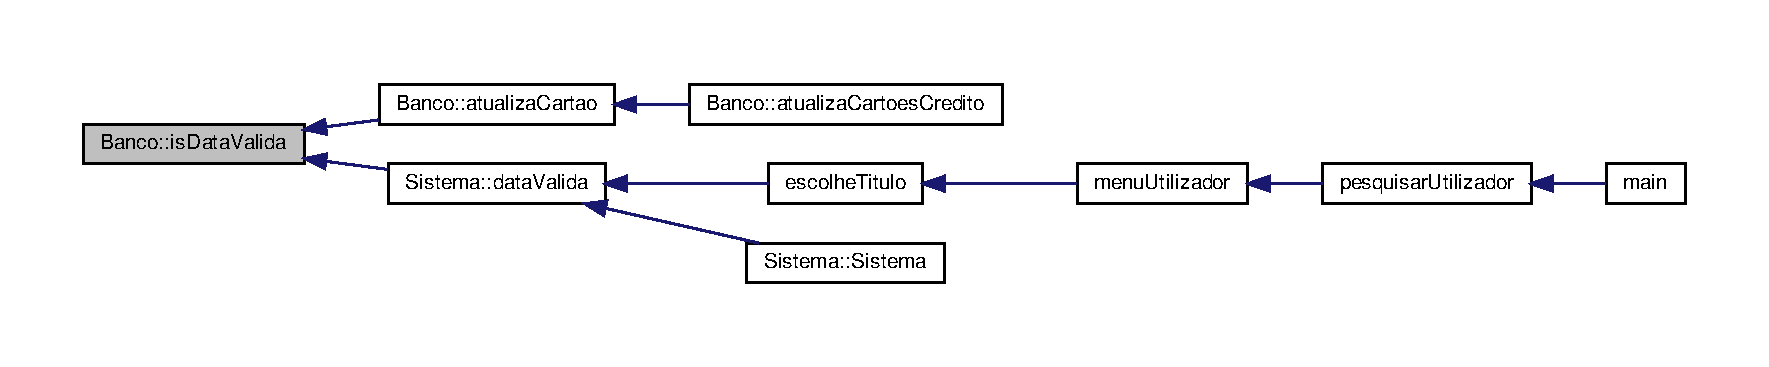
\includegraphics[width=350pt]{classBanco_ac469cc9db5980081701bf9eb27a7e612_icgraph}
\end{center}
\end{figure}
\mbox{\Hypertarget{classBanco_a227af53b49995242c06d89bb10ffc8ea}\label{classBanco_a227af53b49995242c06d89bb10ffc8ea}} 
\index{Banco@{Banco}!set\+Data\+Atual@{set\+Data\+Atual}}
\index{set\+Data\+Atual@{set\+Data\+Atual}!Banco@{Banco}}
\subsubsection{\texorpdfstring{set\+Data\+Atual()}{setDataAtual()}}
{\footnotesize\ttfamily void Banco\+::set\+Data\+Atual (\begin{DoxyParamCaption}{ }\end{DoxyParamCaption})}



atualiza a data, para a data atual 



The documentation for this class was generated from the following files\+:\begin{DoxyCompactItemize}
\item 
\hyperlink{Banco_8h}{Banco.\+h}\item 
\hyperlink{Banco_8cpp}{Banco.\+cpp}\end{DoxyCompactItemize}

\hypertarget{classBiblioteca}{}\section{Biblioteca Class Reference}
\label{classBiblioteca}\index{Biblioteca@{Biblioteca}}


{\ttfamily \#include $<$Biblioteca.\+h$>$}

\subsection*{Public Member Functions}
\begin{DoxyCompactItemize}
\item 
void \hyperlink{classBiblioteca_af10c9f23d85db8e03ae2e8b9d3e593e1}{adiciona\+Titulo} (\hyperlink{classTitulo}{Titulo} $\ast$T)
\begin{DoxyCompactList}\small\item\em Adicona um titulo a biblioteca. \end{DoxyCompactList}\item 
std\+::vector$<$ \hyperlink{classTitulo}{Titulo} $\ast$ $>$ \hyperlink{classBiblioteca_a03c1ebf76a4ace4f57000bb99a87bb88}{get\+Titulos} () const
\begin{DoxyCompactList}\small\item\em Devolve o vetor de titulos. \end{DoxyCompactList}\item 
bool \hyperlink{classBiblioteca_a962423a2d93507ad7348e9b8c83eb1b8}{operator==} (const \hyperlink{classBiblioteca}{Biblioteca} B)
\begin{DoxyCompactList}\small\item\em Overload do operador de igualdade. \end{DoxyCompactList}\end{DoxyCompactItemize}


\subsection{Detailed Description}
Bibloteca que foi declarado no \hyperlink{classUtilizador}{Utilizador} 

\subsection{Member Function Documentation}
\mbox{\Hypertarget{classBiblioteca_af10c9f23d85db8e03ae2e8b9d3e593e1}\label{classBiblioteca_af10c9f23d85db8e03ae2e8b9d3e593e1}} 
\index{Biblioteca@{Biblioteca}!adiciona\+Titulo@{adiciona\+Titulo}}
\index{adiciona\+Titulo@{adiciona\+Titulo}!Biblioteca@{Biblioteca}}
\subsubsection{\texorpdfstring{adiciona\+Titulo()}{adicionaTitulo()}}
{\footnotesize\ttfamily void Biblioteca\+::adiciona\+Titulo (\begin{DoxyParamCaption}\item[{\hyperlink{classTitulo}{Titulo} $\ast$}]{T }\end{DoxyParamCaption})}



Adicona um titulo a biblioteca. 


\begin{DoxyParams}{Parameters}
{\em T} & -\/ \hyperlink{classTitulo}{Titulo} a adicionar \\
\hline
\end{DoxyParams}

\begin{DoxyCode}
5                                           \{
6     \textcolor{keywordflow}{for} (\textcolor{keywordtype}{size\_t} i = 0; i < titulos.size(); i++) \{
7         \textcolor{keywordflow}{if} (titulos[i]->getNome() == T->\hyperlink{classTitulo_acb79279860b3404c6419697df5f860cb}{getNome}() && titulos[i]->getPlataforma() == T->
      \hyperlink{classTitulo_a2a57a31d40c5df012b3c6e2451c253dd}{getPlataforma}()) \{
8             \textcolor{keywordflow}{throw} \hyperlink{classTituloJaAdicionado}{TituloJaAdicionado}(\textcolor{stringliteral}{"Jogo ja adicionado"});
9         \}
10     \}
11     titulos.push\_back(T);
12 \}
\end{DoxyCode}
Here is the call graph for this function\+:
\nopagebreak
\begin{figure}[H]
\begin{center}
\leavevmode
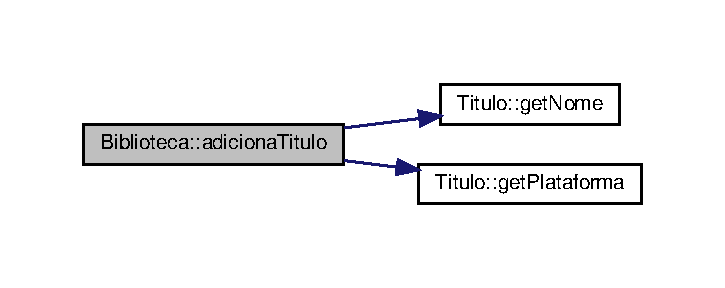
\includegraphics[width=348pt]{classBiblioteca_af10c9f23d85db8e03ae2e8b9d3e593e1_cgraph}
\end{center}
\end{figure}
Here is the caller graph for this function\+:
\nopagebreak
\begin{figure}[H]
\begin{center}
\leavevmode
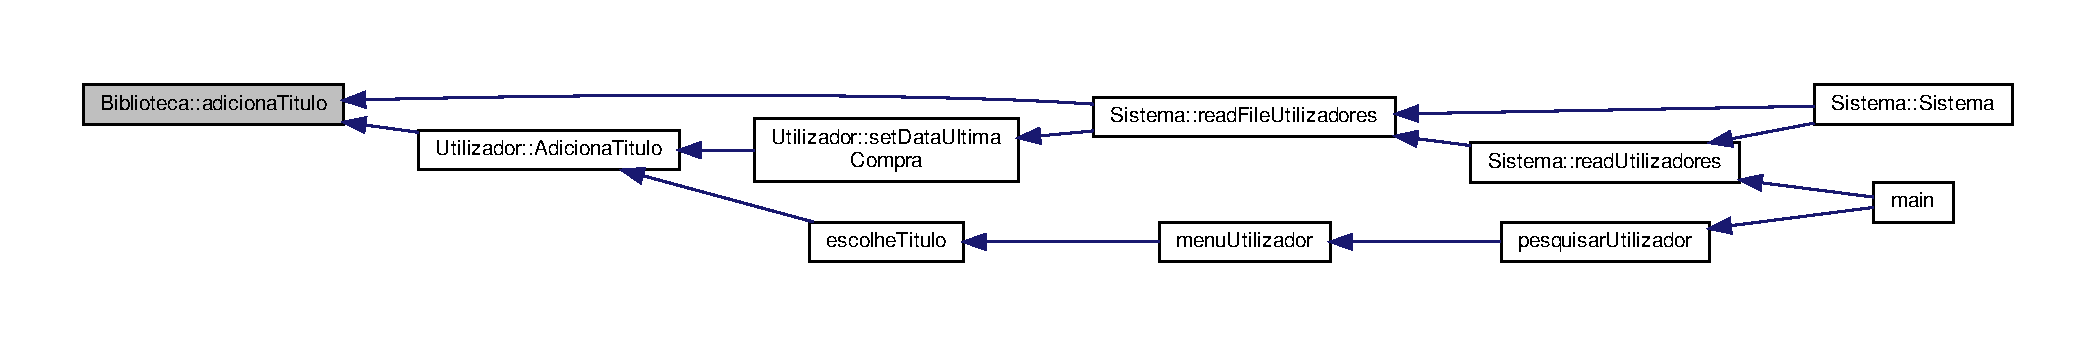
\includegraphics[width=350pt]{classBiblioteca_af10c9f23d85db8e03ae2e8b9d3e593e1_icgraph}
\end{center}
\end{figure}
\mbox{\Hypertarget{classBiblioteca_a03c1ebf76a4ace4f57000bb99a87bb88}\label{classBiblioteca_a03c1ebf76a4ace4f57000bb99a87bb88}} 
\index{Biblioteca@{Biblioteca}!get\+Titulos@{get\+Titulos}}
\index{get\+Titulos@{get\+Titulos}!Biblioteca@{Biblioteca}}
\subsubsection{\texorpdfstring{get\+Titulos()}{getTitulos()}}
{\footnotesize\ttfamily std\+::vector$<$ \hyperlink{classTitulo}{Titulo} $\ast$ $>$ Biblioteca\+::get\+Titulos (\begin{DoxyParamCaption}{ }\end{DoxyParamCaption}) const}



Devolve o vetor de titulos. 

\begin{DoxyReturn}{Returns}
Retorna vetor de titulos da biblioteca 
\end{DoxyReturn}

\begin{DoxyCode}
15 \{
16     \textcolor{keywordflow}{return} titulos;
17 \}
\end{DoxyCode}
Here is the caller graph for this function\+:
\nopagebreak
\begin{figure}[H]
\begin{center}
\leavevmode
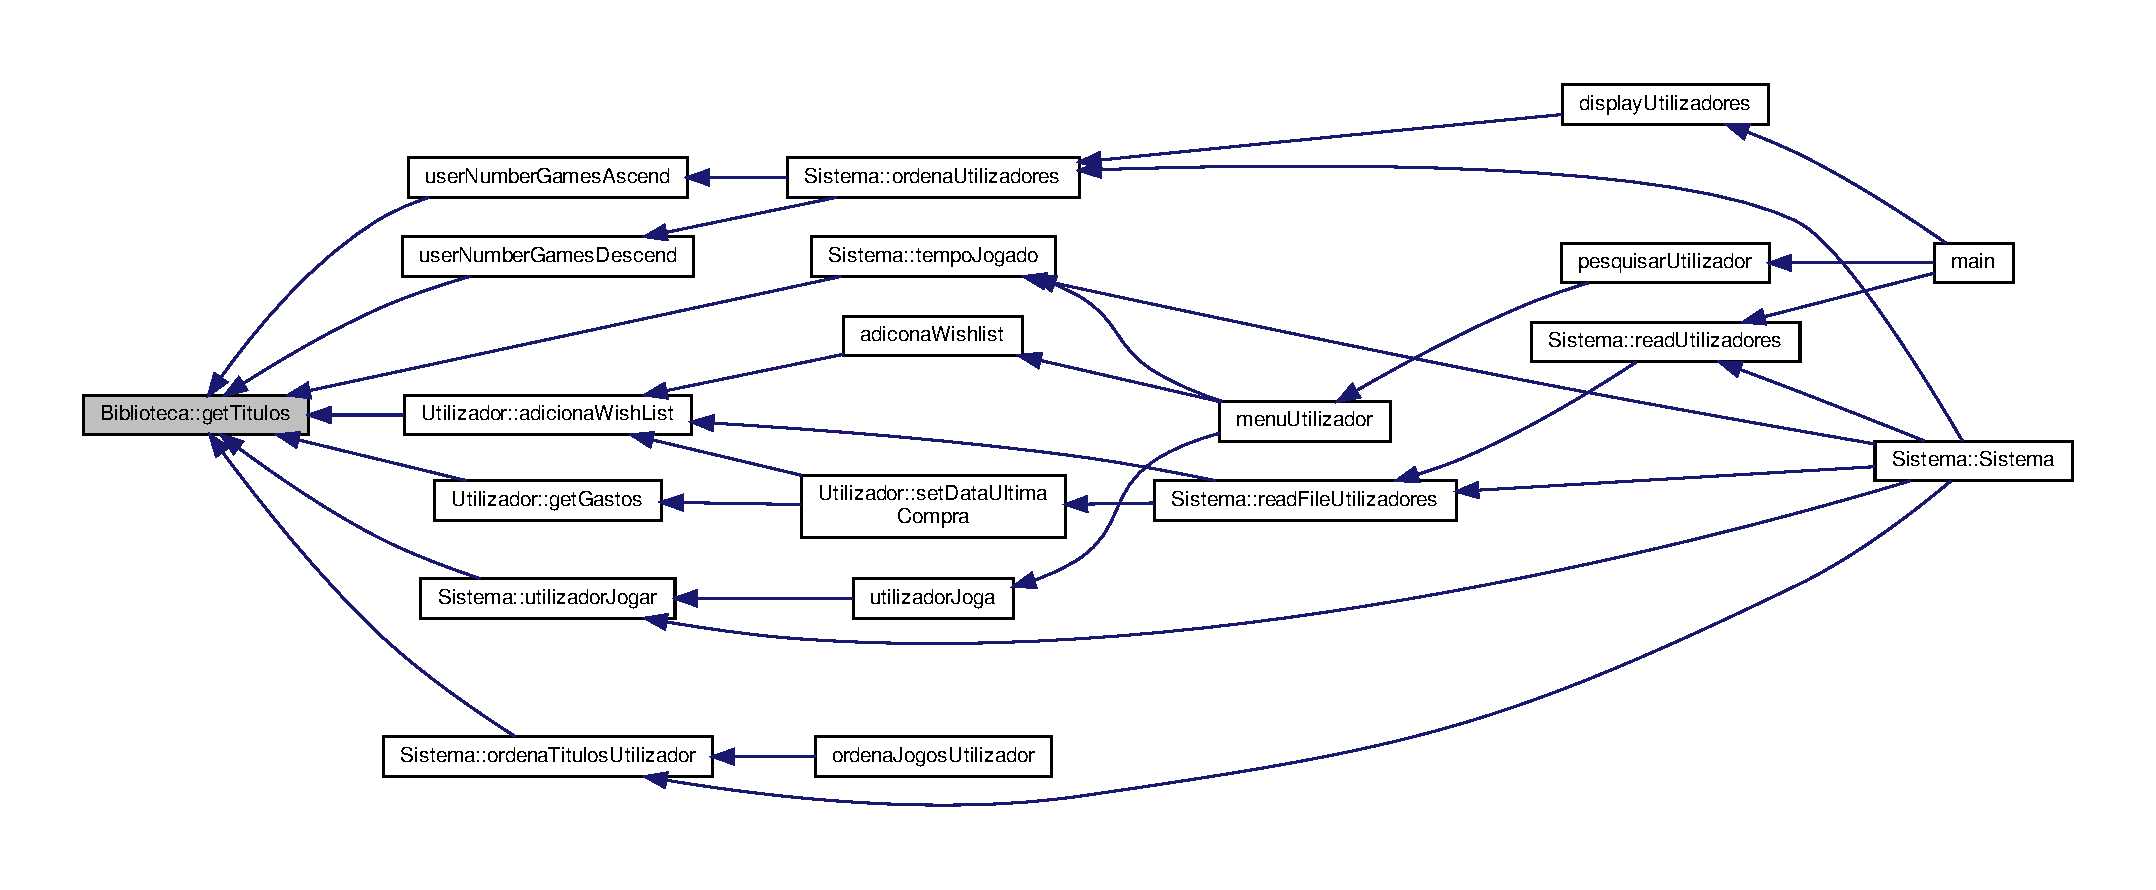
\includegraphics[width=350pt]{classBiblioteca_a03c1ebf76a4ace4f57000bb99a87bb88_icgraph}
\end{center}
\end{figure}
\mbox{\Hypertarget{classBiblioteca_a962423a2d93507ad7348e9b8c83eb1b8}\label{classBiblioteca_a962423a2d93507ad7348e9b8c83eb1b8}} 
\index{Biblioteca@{Biblioteca}!operator==@{operator==}}
\index{operator==@{operator==}!Biblioteca@{Biblioteca}}
\subsubsection{\texorpdfstring{operator==()}{operator==()}}
{\footnotesize\ttfamily bool Biblioteca\+::operator== (\begin{DoxyParamCaption}\item[{const \hyperlink{classBiblioteca}{Biblioteca}}]{B }\end{DoxyParamCaption})}



Overload do operador de igualdade. 


\begin{DoxyParams}{Parameters}
{\em B} & -\/ \hyperlink{classBiblioteca}{Biblioteca} a ser comparada \\
\hline
\end{DoxyParams}

\begin{DoxyCode}
20 \{
21     \textcolor{keywordflow}{return} this->titulos==B.titulos;
22 \}
\end{DoxyCode}


The documentation for this class was generated from the following files\+:\begin{DoxyCompactItemize}
\item 
\hyperlink{Biblioteca_8h}{Biblioteca.\+h}\item 
\hyperlink{Biblioteca_8cpp}{Biblioteca.\+cpp}\end{DoxyCompactItemize}

\hypertarget{classCartaoCredito}{}\section{Cartao\+Credito Class Reference}
\label{classCartaoCredito}\index{Cartao\+Credito@{Cartao\+Credito}}


{\ttfamily \#include $<$Cartao\+Credito.\+h$>$}

\subsection*{Public Member Functions}
\begin{DoxyCompactItemize}
\item 
\hyperlink{classCartaoCredito_a49b6298290f8307df4a42b15175fb10f}{Cartao\+Credito} (const float saldo=0, const \hyperlink{classData}{Data} \&d1=\hyperlink{classData}{Data}(), const std\+::string iD=\char`\"{}\char`\"{})
\begin{DoxyCompactList}\small\item\em Construtor da classe Cartao de credito. \end{DoxyCompactList}\item 
float \hyperlink{classCartaoCredito_a5d10788d907961f86779efaecb6a231d}{get\+Saldo} () const
\begin{DoxyCompactList}\small\item\em devolve o saldo do cartao \end{DoxyCompactList}\item 
\hyperlink{classData}{Data} \hyperlink{classCartaoCredito_ab28b73bbecc20b5c23348e1172230533}{get\+Data\+De\+Validade} () const
\begin{DoxyCompactList}\small\item\em Devolve a data de validade do cartao. \end{DoxyCompactList}\item 
std\+::string \hyperlink{classCartaoCredito_ab59d60e4d155e7f29aef888ea3139ee5}{get\+Id} () const
\begin{DoxyCompactList}\small\item\em Devolve o id(string) do cartao de credito atual. \end{DoxyCompactList}\item 
void \hyperlink{classCartaoCredito_a52daaab859e37d416c00044ef0fb2f27}{atualiza\+Data\+De\+Validade} ()
\begin{DoxyCompactList}\small\item\em Atualiza a data de validade para a data atual. \end{DoxyCompactList}\item 
bool \hyperlink{classCartaoCredito_abf34d4aff89aac4b76d9e15999d85a26}{operator==} (const \hyperlink{classCartaoCredito}{Cartao\+Credito} \&C) const
\begin{DoxyCompactList}\small\item\em Overload do operador de igualdade. \end{DoxyCompactList}\item 
void \hyperlink{classCartaoCredito_a03d4e7d9d645737bc3d162daf3555e25}{adiciona\+Quantia} (float quantia)
\begin{DoxyCompactList}\small\item\em Adiciona uma quantia ao saldo do cartao. \end{DoxyCompactList}\item 
void \hyperlink{classCartaoCredito_a57d3f8baa86eb9a8f348dc7cbc91ea42}{remove\+Quantia} (float quantia)
\begin{DoxyCompactList}\small\item\em Remove uma quantia ao saldo. \end{DoxyCompactList}\end{DoxyCompactItemize}


\subsection{Detailed Description}
Classe \hyperlink{classCartaoCredito}{Cartao\+Credito} utilizada na classe \hyperlink{classUtilizador}{Utilizador} 

\subsection{Constructor \& Destructor Documentation}
\mbox{\Hypertarget{classCartaoCredito_a49b6298290f8307df4a42b15175fb10f}\label{classCartaoCredito_a49b6298290f8307df4a42b15175fb10f}} 
\index{Cartao\+Credito@{Cartao\+Credito}!Cartao\+Credito@{Cartao\+Credito}}
\index{Cartao\+Credito@{Cartao\+Credito}!Cartao\+Credito@{Cartao\+Credito}}
\subsubsection{\texorpdfstring{Cartao\+Credito()}{CartaoCredito()}}
{\footnotesize\ttfamily Cartao\+Credito\+::\+Cartao\+Credito (\begin{DoxyParamCaption}\item[{const float}]{saldo = {\ttfamily 0},  }\item[{const \hyperlink{classData}{Data} \&}]{d1 = {\ttfamily \hyperlink{classData}{Data}()},  }\item[{const std\+::string}]{iD = {\ttfamily \char`\"{}\char`\"{}} }\end{DoxyParamCaption})}



Construtor da classe Cartao de credito. 


\begin{DoxyParams}{Parameters}
{\em saldo} & -\/ Saldo a atribuir ao cartao \\
\hline
{\em d1} & -\/ \hyperlink{classData}{Data} da validade do Cartao \\
\hline
{\em iD} & -\/ Identificador a atribuir ao cartao \\
\hline
\end{DoxyParams}

\begin{DoxyCode}
9 : id(iD) \textcolor{comment}{/* id deve ser diferente de todos os cartoes*/}
10 \{
11     this->saldo=saldo;
12     this->dataDeValidade = d1;
13 
14 \}
\end{DoxyCode}


\subsection{Member Function Documentation}
\mbox{\Hypertarget{classCartaoCredito_a03d4e7d9d645737bc3d162daf3555e25}\label{classCartaoCredito_a03d4e7d9d645737bc3d162daf3555e25}} 
\index{Cartao\+Credito@{Cartao\+Credito}!adiciona\+Quantia@{adiciona\+Quantia}}
\index{adiciona\+Quantia@{adiciona\+Quantia}!Cartao\+Credito@{Cartao\+Credito}}
\subsubsection{\texorpdfstring{adiciona\+Quantia()}{adicionaQuantia()}}
{\footnotesize\ttfamily void Cartao\+Credito\+::adiciona\+Quantia (\begin{DoxyParamCaption}\item[{float}]{quantia }\end{DoxyParamCaption})}



Adiciona uma quantia ao saldo do cartao. 


\begin{DoxyCode}
45 \{
46     this->saldo += quantia;
47 \}
\end{DoxyCode}
\mbox{\Hypertarget{classCartaoCredito_a52daaab859e37d416c00044ef0fb2f27}\label{classCartaoCredito_a52daaab859e37d416c00044ef0fb2f27}} 
\index{Cartao\+Credito@{Cartao\+Credito}!atualiza\+Data\+De\+Validade@{atualiza\+Data\+De\+Validade}}
\index{atualiza\+Data\+De\+Validade@{atualiza\+Data\+De\+Validade}!Cartao\+Credito@{Cartao\+Credito}}
\subsubsection{\texorpdfstring{atualiza\+Data\+De\+Validade()}{atualizaDataDeValidade()}}
{\footnotesize\ttfamily void Cartao\+Credito\+::atualiza\+Data\+De\+Validade (\begin{DoxyParamCaption}{ }\end{DoxyParamCaption})}



Atualiza a data de validade para a data atual. 


\begin{DoxyCode}
28 \{
29     this->dataDeValidade.\hyperlink{classData_a8d4cfad647b590df436d8260000a2745}{setAno}(this->dataDeValidade.\hyperlink{classData_ae19e0d5af87f94f2809ba52dae69e15b}{getAno}() + 3);
30 \}
\end{DoxyCode}
Here is the call graph for this function\+:
\nopagebreak
\begin{figure}[H]
\begin{center}
\leavevmode
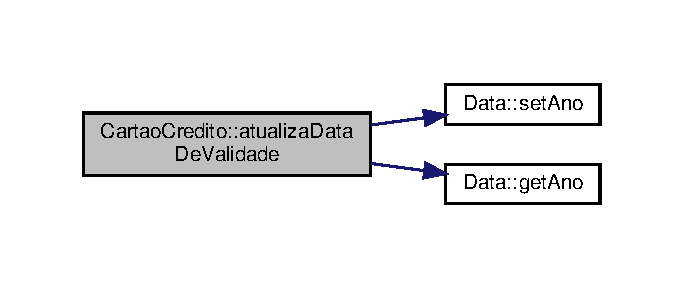
\includegraphics[width=328pt]{classCartaoCredito_a52daaab859e37d416c00044ef0fb2f27_cgraph}
\end{center}
\end{figure}
Here is the caller graph for this function\+:
\nopagebreak
\begin{figure}[H]
\begin{center}
\leavevmode
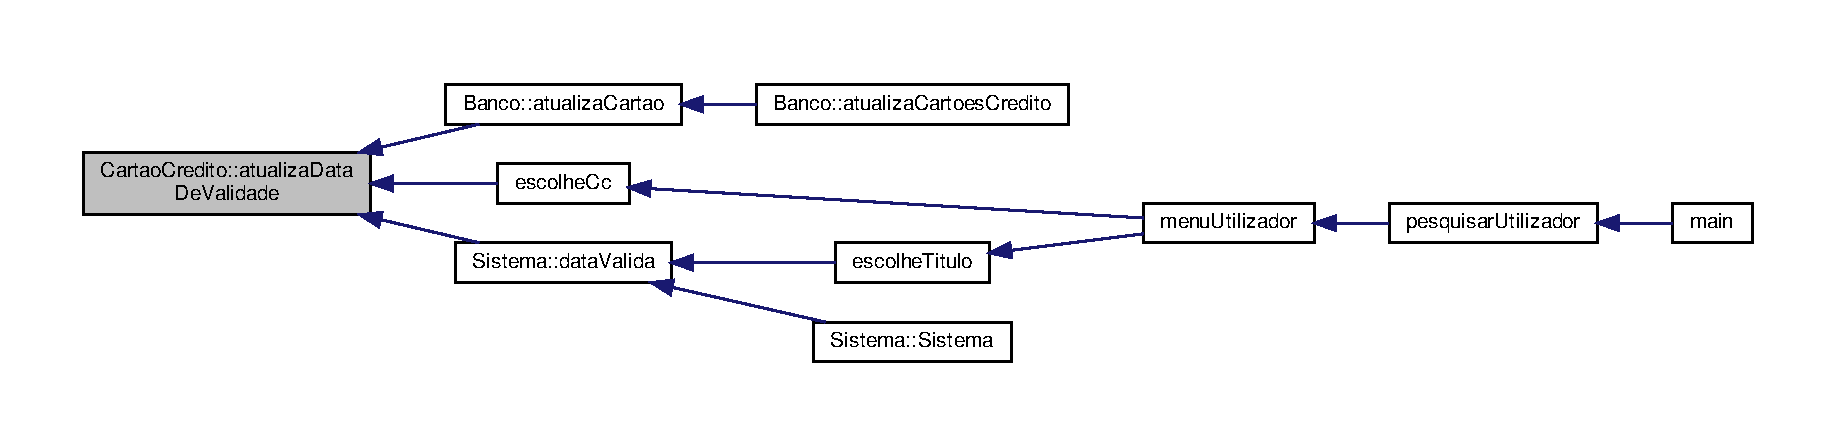
\includegraphics[width=350pt]{classCartaoCredito_a52daaab859e37d416c00044ef0fb2f27_icgraph}
\end{center}
\end{figure}
\mbox{\Hypertarget{classCartaoCredito_ab28b73bbecc20b5c23348e1172230533}\label{classCartaoCredito_ab28b73bbecc20b5c23348e1172230533}} 
\index{Cartao\+Credito@{Cartao\+Credito}!get\+Data\+De\+Validade@{get\+Data\+De\+Validade}}
\index{get\+Data\+De\+Validade@{get\+Data\+De\+Validade}!Cartao\+Credito@{Cartao\+Credito}}
\subsubsection{\texorpdfstring{get\+Data\+De\+Validade()}{getDataDeValidade()}}
{\footnotesize\ttfamily \hyperlink{classData}{Data} Cartao\+Credito\+::get\+Data\+De\+Validade (\begin{DoxyParamCaption}{ }\end{DoxyParamCaption}) const}



Devolve a data de validade do cartao. 

\begin{DoxyReturn}{Returns}
Retorna a data de validade do cartao 
\end{DoxyReturn}

\begin{DoxyCode}
23 \{
24     \textcolor{keywordflow}{return} this->dataDeValidade;
25 \}
\end{DoxyCode}
Here is the caller graph for this function\+:
\nopagebreak
\begin{figure}[H]
\begin{center}
\leavevmode
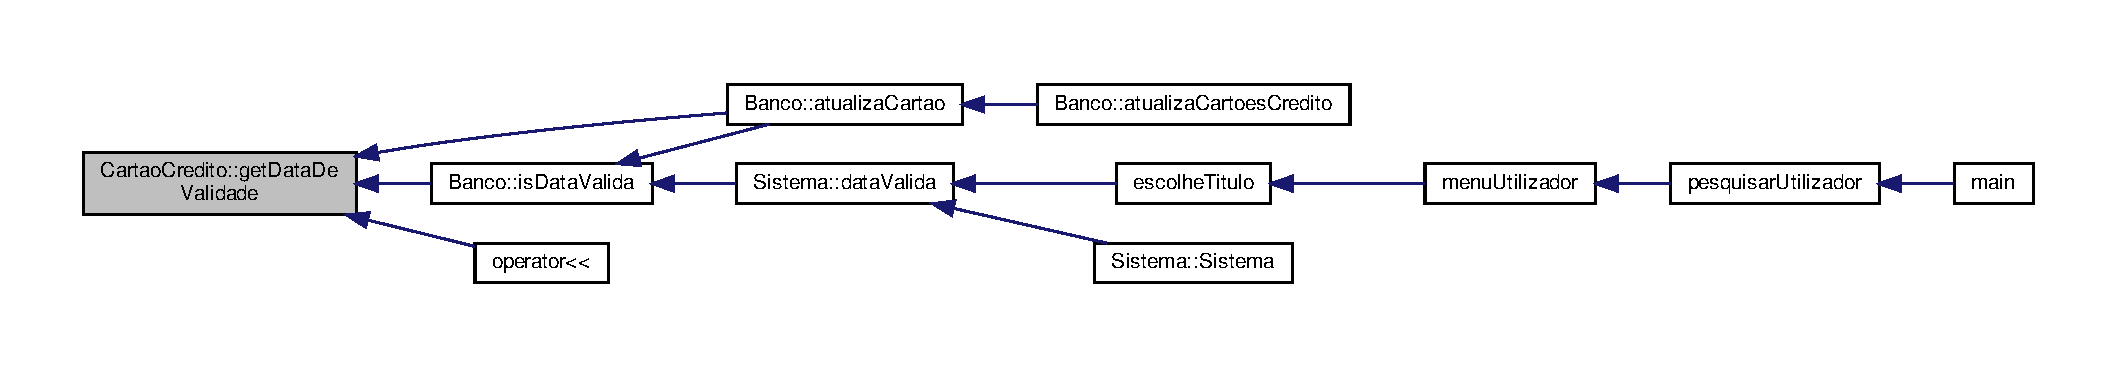
\includegraphics[width=350pt]{classCartaoCredito_ab28b73bbecc20b5c23348e1172230533_icgraph}
\end{center}
\end{figure}
\mbox{\Hypertarget{classCartaoCredito_ab59d60e4d155e7f29aef888ea3139ee5}\label{classCartaoCredito_ab59d60e4d155e7f29aef888ea3139ee5}} 
\index{Cartao\+Credito@{Cartao\+Credito}!get\+Id@{get\+Id}}
\index{get\+Id@{get\+Id}!Cartao\+Credito@{Cartao\+Credito}}
\subsubsection{\texorpdfstring{get\+Id()}{getId()}}
{\footnotesize\ttfamily std\+::string Cartao\+Credito\+::get\+Id (\begin{DoxyParamCaption}{ }\end{DoxyParamCaption}) const}



Devolve o id(string) do cartao de credito atual. 

\begin{DoxyReturn}{Returns}
Retorna o identificador do cartao 
\end{DoxyReturn}

\begin{DoxyCode}
34 \{
35     \textcolor{keywordflow}{return} this->id;
36 \}
\end{DoxyCode}
Here is the caller graph for this function\+:
\nopagebreak
\begin{figure}[H]
\begin{center}
\leavevmode
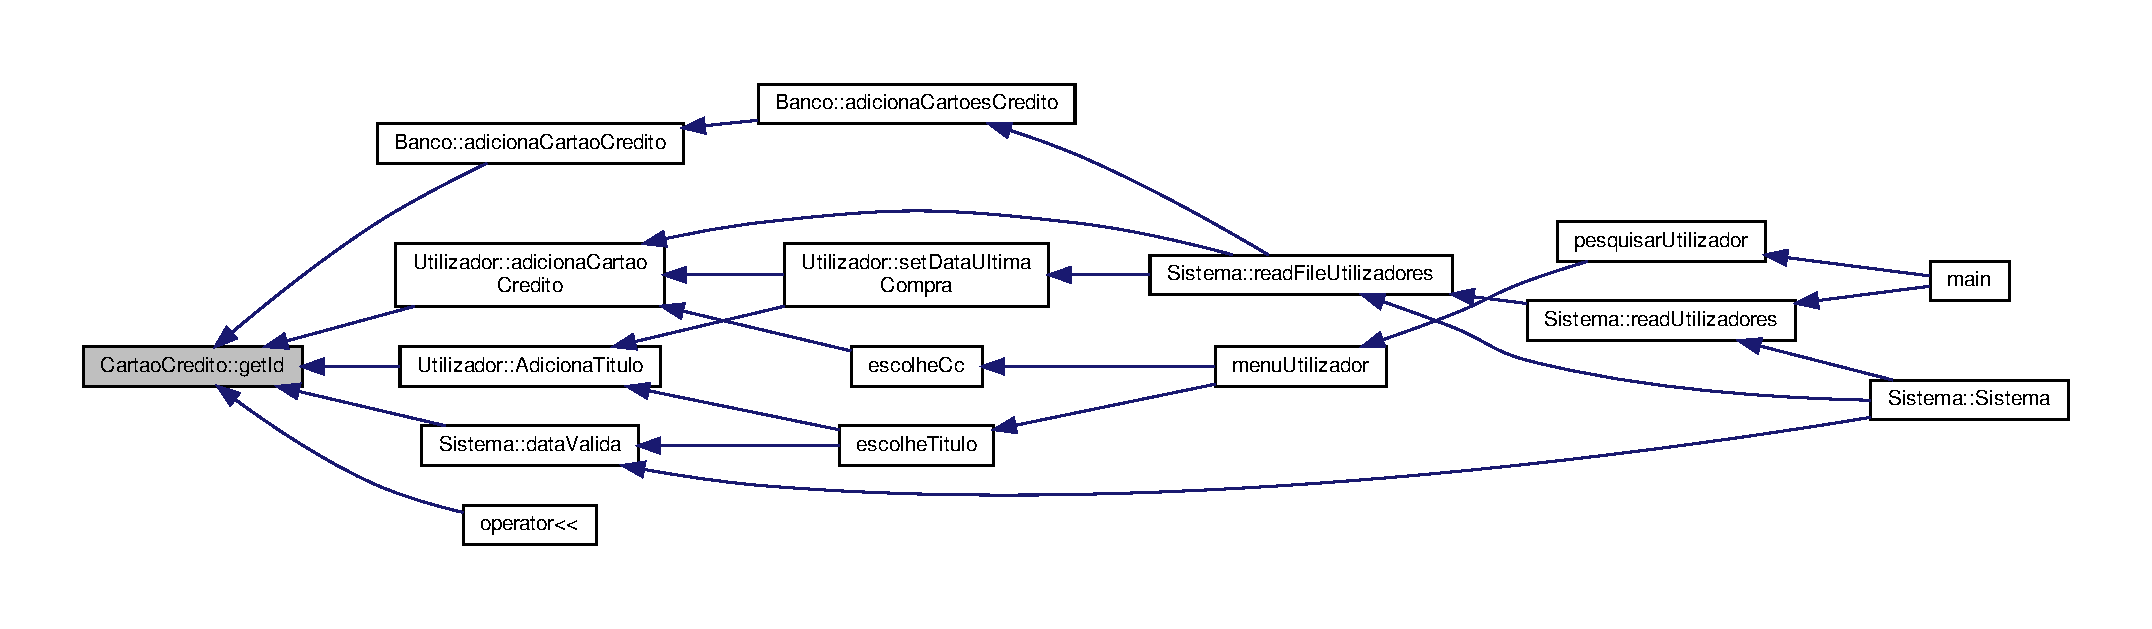
\includegraphics[width=350pt]{classCartaoCredito_ab59d60e4d155e7f29aef888ea3139ee5_icgraph}
\end{center}
\end{figure}
\mbox{\Hypertarget{classCartaoCredito_a5d10788d907961f86779efaecb6a231d}\label{classCartaoCredito_a5d10788d907961f86779efaecb6a231d}} 
\index{Cartao\+Credito@{Cartao\+Credito}!get\+Saldo@{get\+Saldo}}
\index{get\+Saldo@{get\+Saldo}!Cartao\+Credito@{Cartao\+Credito}}
\subsubsection{\texorpdfstring{get\+Saldo()}{getSaldo()}}
{\footnotesize\ttfamily float Cartao\+Credito\+::get\+Saldo (\begin{DoxyParamCaption}{ }\end{DoxyParamCaption}) const}



devolve o saldo do cartao 

\begin{DoxyReturn}{Returns}
Retorna o saldo do utilizador 
\end{DoxyReturn}

\begin{DoxyCode}
17 \{
18     \textcolor{keywordflow}{return} this->saldo;
19 \}
\end{DoxyCode}
Here is the caller graph for this function\+:
\nopagebreak
\begin{figure}[H]
\begin{center}
\leavevmode
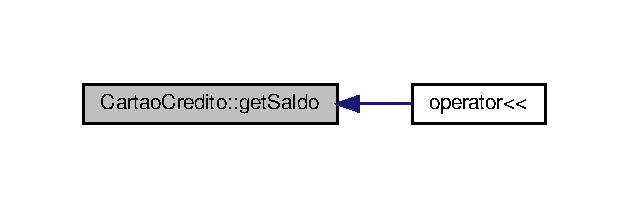
\includegraphics[width=302pt]{classCartaoCredito_a5d10788d907961f86779efaecb6a231d_icgraph}
\end{center}
\end{figure}
\mbox{\Hypertarget{classCartaoCredito_abf34d4aff89aac4b76d9e15999d85a26}\label{classCartaoCredito_abf34d4aff89aac4b76d9e15999d85a26}} 
\index{Cartao\+Credito@{Cartao\+Credito}!operator==@{operator==}}
\index{operator==@{operator==}!Cartao\+Credito@{Cartao\+Credito}}
\subsubsection{\texorpdfstring{operator==()}{operator==()}}
{\footnotesize\ttfamily bool Cartao\+Credito\+::operator== (\begin{DoxyParamCaption}\item[{const \hyperlink{classCartaoCredito}{Cartao\+Credito} \&}]{C }\end{DoxyParamCaption}) const}



Overload do operador de igualdade. 


\begin{DoxyParams}{Parameters}
{\em C} & -\/ cartao de credito a comparar com o objeto atual \\
\hline
\end{DoxyParams}
\begin{DoxyReturn}{Returns}
Retorna verdadeiro se os cartoes sao iguais 
\end{DoxyReturn}

\begin{DoxyCode}
39 \{
40     \textcolor{keywordflow}{return} (this->\textcolor{keywordtype}{id}== C.id);
41 
42 \}
\end{DoxyCode}
\mbox{\Hypertarget{classCartaoCredito_a57d3f8baa86eb9a8f348dc7cbc91ea42}\label{classCartaoCredito_a57d3f8baa86eb9a8f348dc7cbc91ea42}} 
\index{Cartao\+Credito@{Cartao\+Credito}!remove\+Quantia@{remove\+Quantia}}
\index{remove\+Quantia@{remove\+Quantia}!Cartao\+Credito@{Cartao\+Credito}}
\subsubsection{\texorpdfstring{remove\+Quantia()}{removeQuantia()}}
{\footnotesize\ttfamily void Cartao\+Credito\+::remove\+Quantia (\begin{DoxyParamCaption}\item[{float}]{quantia }\end{DoxyParamCaption})}



Remove uma quantia ao saldo. 


\begin{DoxyCode}
50 \{
51     \textcolor{keywordflow}{if} (this->saldo - quantia >= 0)
52         this->saldo -= quantia;
53     \textcolor{keywordflow}{else} \textcolor{keywordflow}{throw} \hyperlink{classSaldoInsuficiente}{SaldoInsuficiente}(\textcolor{stringliteral}{"A quantia "}+std::to\_string(this->saldo)+\textcolor{stringliteral}{" e insuficiente
      "});
54 \}
\end{DoxyCode}


The documentation for this class was generated from the following files\+:\begin{DoxyCompactItemize}
\item 
\hyperlink{CartaoCredito_8h}{Cartao\+Credito.\+h}\item 
\hyperlink{CartaoCredito_8cpp}{Cartao\+Credito.\+cpp}\end{DoxyCompactItemize}

\hypertarget{classCartaoInexistente}{}\section{Cartao\+Inexistente Class Reference}
\label{classCartaoInexistente}\index{Cartao\+Inexistente@{Cartao\+Inexistente}}


{\ttfamily \#include $<$Erro.\+h$>$}



Inheritance diagram for Cartao\+Inexistente\+:
\nopagebreak
\begin{figure}[H]
\begin{center}
\leavevmode
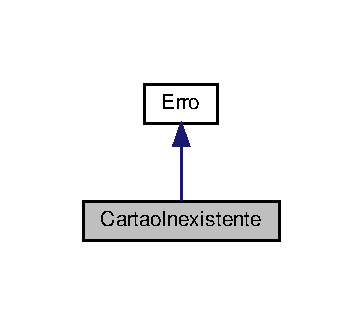
\includegraphics[width=174pt]{classCartaoInexistente__inherit__graph}
\end{center}
\end{figure}


Collaboration diagram for Cartao\+Inexistente\+:
\nopagebreak
\begin{figure}[H]
\begin{center}
\leavevmode
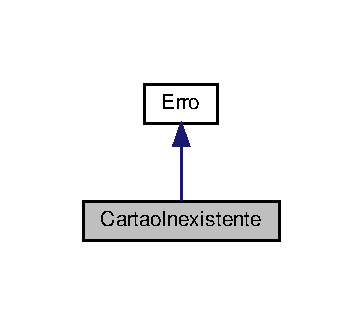
\includegraphics[width=174pt]{classCartaoInexistente__coll__graph}
\end{center}
\end{figure}
\subsection*{Public Member Functions}
\begin{DoxyCompactItemize}
\item 
\hyperlink{classCartaoInexistente_a48a83d627aabc141aa1bb7216c74918b}{Cartao\+Inexistente} (const std\+::string \&info)
\begin{DoxyCompactList}\small\item\em Construtor da classe \hyperlink{classCartaoInexistente}{Cartao\+Inexistente}. \end{DoxyCompactList}\end{DoxyCompactItemize}


\subsection{Constructor \& Destructor Documentation}
\mbox{\Hypertarget{classCartaoInexistente_a48a83d627aabc141aa1bb7216c74918b}\label{classCartaoInexistente_a48a83d627aabc141aa1bb7216c74918b}} 
\index{Cartao\+Inexistente@{Cartao\+Inexistente}!Cartao\+Inexistente@{Cartao\+Inexistente}}
\index{Cartao\+Inexistente@{Cartao\+Inexistente}!Cartao\+Inexistente@{Cartao\+Inexistente}}
\subsubsection{\texorpdfstring{Cartao\+Inexistente()}{CartaoInexistente()}}
{\footnotesize\ttfamily Cartao\+Inexistente\+::\+Cartao\+Inexistente (\begin{DoxyParamCaption}\item[{const std\+::string \&}]{info }\end{DoxyParamCaption})\hspace{0.3cm}{\ttfamily [inline]}}



Construtor da classe \hyperlink{classCartaoInexistente}{Cartao\+Inexistente}. 


\begin{DoxyCode}
92 : \hyperlink{classErro_a15d79796bd17517ff05d45eee55556f1}{Erro}(info) \{ \}
\end{DoxyCode}


The documentation for this class was generated from the following file\+:\begin{DoxyCompactItemize}
\item 
\hyperlink{Erro_8h}{Erro.\+h}\end{DoxyCompactItemize}

\hypertarget{classCartaoInvalido}{}\section{Cartao\+Invalido Class Reference}
\label{classCartaoInvalido}\index{Cartao\+Invalido@{Cartao\+Invalido}}


{\ttfamily \#include $<$Erro.\+h$>$}



Inheritance diagram for Cartao\+Invalido\+:
\nopagebreak
\begin{figure}[H]
\begin{center}
\leavevmode
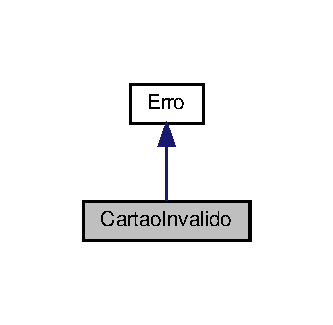
\includegraphics[width=160pt]{classCartaoInvalido__inherit__graph}
\end{center}
\end{figure}


Collaboration diagram for Cartao\+Invalido\+:
\nopagebreak
\begin{figure}[H]
\begin{center}
\leavevmode
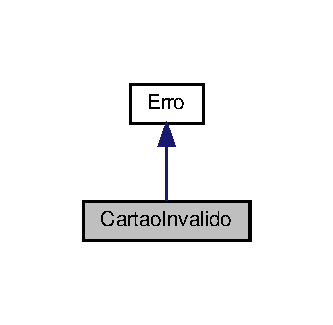
\includegraphics[width=160pt]{classCartaoInvalido__coll__graph}
\end{center}
\end{figure}
\subsection*{Public Member Functions}
\begin{DoxyCompactItemize}
\item 
\hyperlink{classCartaoInvalido_a24653e20aedf639b42cd9ed8a56bdc83}{Cartao\+Invalido} (const std\+::string \&info)
\begin{DoxyCompactList}\small\item\em Construtor da classe \hyperlink{classCartaoInvalido}{Cartao\+Invalido}. \end{DoxyCompactList}\end{DoxyCompactItemize}


\subsection{Constructor \& Destructor Documentation}
\mbox{\Hypertarget{classCartaoInvalido_a24653e20aedf639b42cd9ed8a56bdc83}\label{classCartaoInvalido_a24653e20aedf639b42cd9ed8a56bdc83}} 
\index{Cartao\+Invalido@{Cartao\+Invalido}!Cartao\+Invalido@{Cartao\+Invalido}}
\index{Cartao\+Invalido@{Cartao\+Invalido}!Cartao\+Invalido@{Cartao\+Invalido}}
\subsubsection{\texorpdfstring{Cartao\+Invalido()}{CartaoInvalido()}}
{\footnotesize\ttfamily Cartao\+Invalido\+::\+Cartao\+Invalido (\begin{DoxyParamCaption}\item[{const std\+::string \&}]{info }\end{DoxyParamCaption})\hspace{0.3cm}{\ttfamily [inline]}}



Construtor da classe \hyperlink{classCartaoInvalido}{Cartao\+Invalido}. 


\begin{DoxyCode}
114 : \hyperlink{classErro_a15d79796bd17517ff05d45eee55556f1}{Erro}(info) \{ \}
\end{DoxyCode}


The documentation for this class was generated from the following file\+:\begin{DoxyCompactItemize}
\item 
\hyperlink{Erro_8h}{Erro.\+h}\end{DoxyCompactItemize}

\hypertarget{classCartaoJaExistente}{}\section{Cartao\+Ja\+Existente Class Reference}
\label{classCartaoJaExistente}\index{Cartao\+Ja\+Existente@{Cartao\+Ja\+Existente}}


{\ttfamily \#include $<$Erro.\+h$>$}



Inheritance diagram for Cartao\+Ja\+Existente\+:
\nopagebreak
\begin{figure}[H]
\begin{center}
\leavevmode
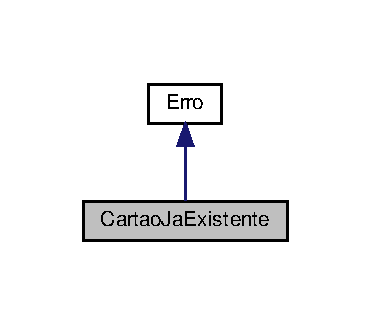
\includegraphics[width=178pt]{classCartaoJaExistente__inherit__graph}
\end{center}
\end{figure}


Collaboration diagram for Cartao\+Ja\+Existente\+:
\nopagebreak
\begin{figure}[H]
\begin{center}
\leavevmode
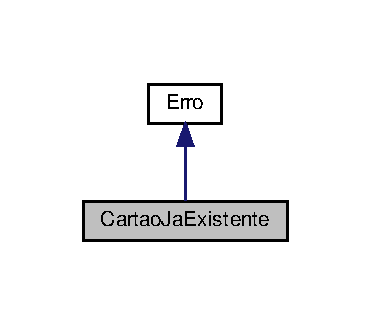
\includegraphics[width=178pt]{classCartaoJaExistente__coll__graph}
\end{center}
\end{figure}
\subsection*{Public Member Functions}
\begin{DoxyCompactItemize}
\item 
\hyperlink{classCartaoJaExistente_ab3efa558a7577d97eff97b81aabc1647}{Cartao\+Ja\+Existente} (const std\+::string \&info)
\begin{DoxyCompactList}\small\item\em Construtor da classe \hyperlink{classCartaoJaExistente}{Cartao\+Ja\+Existente}. \end{DoxyCompactList}\end{DoxyCompactItemize}


\subsection{Constructor \& Destructor Documentation}
\mbox{\Hypertarget{classCartaoJaExistente_ab3efa558a7577d97eff97b81aabc1647}\label{classCartaoJaExistente_ab3efa558a7577d97eff97b81aabc1647}} 
\index{Cartao\+Ja\+Existente@{Cartao\+Ja\+Existente}!Cartao\+Ja\+Existente@{Cartao\+Ja\+Existente}}
\index{Cartao\+Ja\+Existente@{Cartao\+Ja\+Existente}!Cartao\+Ja\+Existente@{Cartao\+Ja\+Existente}}
\subsubsection{\texorpdfstring{Cartao\+Ja\+Existente()}{CartaoJaExistente()}}
{\footnotesize\ttfamily Cartao\+Ja\+Existente\+::\+Cartao\+Ja\+Existente (\begin{DoxyParamCaption}\item[{const std\+::string \&}]{info }\end{DoxyParamCaption})\hspace{0.3cm}{\ttfamily [inline]}}



Construtor da classe \hyperlink{classCartaoJaExistente}{Cartao\+Ja\+Existente}. 


\begin{DoxyCode}
103 : \hyperlink{classErro_a15d79796bd17517ff05d45eee55556f1}{Erro}(info) \{ \}
\end{DoxyCode}


The documentation for this class was generated from the following file\+:\begin{DoxyCompactItemize}
\item 
\hyperlink{Erro_8h}{Erro.\+h}\end{DoxyCompactItemize}

\hypertarget{structcontactos}{}\section{contactos Struct Reference}
\label{structcontactos}\index{contactos@{contactos}}


{\ttfamily \#include $<$Empresa.\+h$>$}

\subsection*{Public Attributes}
\begin{DoxyCompactItemize}
\item 
std\+::string \mbox{\hyperlink{structcontactos_a86c1ad3bcc23dbb8bf7bb37ae0976242}{email}}
\item 
std\+::string \mbox{\hyperlink{structcontactos_a09e1d4029e1eb91fc9ec76e4b4b6d48a}{numero\+Telemovel}}
\end{DoxyCompactItemize}


\subsection{Member Data Documentation}
\mbox{\Hypertarget{structcontactos_a86c1ad3bcc23dbb8bf7bb37ae0976242}\label{structcontactos_a86c1ad3bcc23dbb8bf7bb37ae0976242}} 
\index{contactos@{contactos}!email@{email}}
\index{email@{email}!contactos@{contactos}}
\subsubsection{\texorpdfstring{email}{email}}
{\footnotesize\ttfamily std\+::string contactos\+::email}

\mbox{\Hypertarget{structcontactos_a09e1d4029e1eb91fc9ec76e4b4b6d48a}\label{structcontactos_a09e1d4029e1eb91fc9ec76e4b4b6d48a}} 
\index{contactos@{contactos}!numero\+Telemovel@{numero\+Telemovel}}
\index{numero\+Telemovel@{numero\+Telemovel}!contactos@{contactos}}
\subsubsection{\texorpdfstring{numero\+Telemovel}{numeroTelemovel}}
{\footnotesize\ttfamily std\+::string contactos\+::numero\+Telemovel}



The documentation for this struct was generated from the following file\+:\begin{DoxyCompactItemize}
\item 
\mbox{\hyperlink{_empresa_8h}{Empresa.\+h}}\end{DoxyCompactItemize}

\hypertarget{classData}{}\section{Data Class Reference}
\label{classData}\index{Data@{Data}}


{\ttfamily \#include $<$Data.\+h$>$}

\subsection*{Public Member Functions}
\begin{DoxyCompactItemize}
\item 
\hyperlink{classData_aef12795194c8980d7e9f563f3d9d6c8e}{Data} (unsigned int dia=1, unsigned int mes=1, unsigned int ano=2000)
\begin{DoxyCompactList}\small\item\em Construtor da classe \hyperlink{classData}{Data}. \end{DoxyCompactList}\item 
\hyperlink{classData_a972911ca68256147a714d91bba1e4da2}{Data} (std\+::string data)
\begin{DoxyCompactList}\small\item\em Construtor da classe \hyperlink{classData}{Data} com parametros diferentes. \end{DoxyCompactList}\item 
\hyperlink{classData}{Data} \& \hyperlink{classData_a3e2c5356bc8d548b75c7d085f7a7c4ee}{set\+Dia} (const unsigned int dia)
\begin{DoxyCompactList}\small\item\em Altera o dia. \end{DoxyCompactList}\item 
\hyperlink{classData}{Data} \& \hyperlink{classData_ab15051ae481d89d057b22abc8152584c}{set\+Mes} (const unsigned int mes)
\begin{DoxyCompactList}\small\item\em Altera o mes. \end{DoxyCompactList}\item 
\hyperlink{classData}{Data} \& \hyperlink{classData_a8d4cfad647b590df436d8260000a2745}{set\+Ano} (const unsigned int ano)
\begin{DoxyCompactList}\small\item\em Altera o dia. \end{DoxyCompactList}\item 
unsigned int \hyperlink{classData_a459536c9351759b5697ba25456d9bd70}{get\+Dia} () const
\begin{DoxyCompactList}\small\item\em Devolve o dia. \end{DoxyCompactList}\item 
unsigned int \hyperlink{classData_ab991d6a069c799930899b39bef9a4662}{get\+Mes} () const
\begin{DoxyCompactList}\small\item\em Devolve o mes. \end{DoxyCompactList}\item 
unsigned int \hyperlink{classData_ae19e0d5af87f94f2809ba52dae69e15b}{get\+Ano} () const
\begin{DoxyCompactList}\small\item\em Devolve o ano. \end{DoxyCompactList}\item 
unsigned int \hyperlink{classData_a495d15dd0d90b595740f6e09fd0a2177}{diferenca\+Entre\+Datas} (const \hyperlink{classData}{Data} \&data)
\begin{DoxyCompactList}\small\item\em Calcula a diferen�a de duas datas, em dias. \end{DoxyCompactList}\item 
bool \hyperlink{classData_a8c3fdab05b3e81bb7b302b1d4d9a9d1f}{operator$<$=} (const \hyperlink{classData}{Data} \&D1) const
\begin{DoxyCompactList}\small\item\em Overload do operador $<$= que compara duas data. \end{DoxyCompactList}\item 
bool \hyperlink{classData_a28b51c511a389cf30b9d1d2da858f3f6}{operator$<$} (const \hyperlink{classData}{Data} \&D1) const
\begin{DoxyCompactList}\small\item\em Overload do operador $<$ que compara duas data. \end{DoxyCompactList}\item 
bool \hyperlink{classData_af00bf4efbd3504689f6bc7283378ba5f}{operator==} (const \hyperlink{classData}{Data} \&D1) const
\begin{DoxyCompactList}\small\item\em overload do operador == que compara duas data \end{DoxyCompactList}\end{DoxyCompactItemize}


\subsection{Detailed Description}
Classe data utilizada nos titulos 

\subsection{Constructor \& Destructor Documentation}
\mbox{\Hypertarget{classData_aef12795194c8980d7e9f563f3d9d6c8e}\label{classData_aef12795194c8980d7e9f563f3d9d6c8e}} 
\index{Data@{Data}!Data@{Data}}
\index{Data@{Data}!Data@{Data}}
\subsubsection{\texorpdfstring{Data()}{Data()}\hspace{0.1cm}{\footnotesize\ttfamily [1/2]}}
{\footnotesize\ttfamily Data\+::\+Data (\begin{DoxyParamCaption}\item[{unsigned int}]{dia = {\ttfamily 1},  }\item[{unsigned int}]{mes = {\ttfamily 1},  }\item[{unsigned int}]{ano = {\ttfamily 2000} }\end{DoxyParamCaption})}



Construtor da classe \hyperlink{classData}{Data}. 


\begin{DoxyParams}{Parameters}
{\em d} & -\/ dia \\
\hline
{\em m} & -\/ mes \\
\hline
{\em a} & -\/ ano \\
\hline
\end{DoxyParams}

\begin{DoxyCode}
6                                                                \{
7 
8     this->dia = dia;
9     this->mes = mes;
10     this->ano = ano;
11 \}
\end{DoxyCode}
\mbox{\Hypertarget{classData_a972911ca68256147a714d91bba1e4da2}\label{classData_a972911ca68256147a714d91bba1e4da2}} 
\index{Data@{Data}!Data@{Data}}
\index{Data@{Data}!Data@{Data}}
\subsubsection{\texorpdfstring{Data()}{Data()}\hspace{0.1cm}{\footnotesize\ttfamily [2/2]}}
{\footnotesize\ttfamily Data\+::\+Data (\begin{DoxyParamCaption}\item[{std\+::string}]{data }\end{DoxyParamCaption})}



Construtor da classe \hyperlink{classData}{Data} com parametros diferentes. 


\begin{DoxyParams}{Parameters}
{\em data} & -\/ string a ser tranformada em data \\
\hline
\end{DoxyParams}

\begin{DoxyCode}
13                          \{
14 
15     std::string diaStr = data.substr(0,2);
16     diaStr.erase(0, std::min(diaStr.find\_first\_not\_of(\textcolor{charliteral}{'0'}), diaStr.size()-1));
17     this->dia = std::stoul(diaStr, NULL, 0);
18 
19     std::string mesStr = data.substr(3,2);
20         mesStr.erase(0, std::min(mesStr.find\_first\_not\_of(\textcolor{charliteral}{'0'}), mesStr.size()-1));
21     this->mes = std::stoul( mesStr, NULL, 0);
22 
23     this->ano = std::stoul(data.substr(6,4), NULL, 0);
24 \}
\end{DoxyCode}


\subsection{Member Function Documentation}
\mbox{\Hypertarget{classData_a495d15dd0d90b595740f6e09fd0a2177}\label{classData_a495d15dd0d90b595740f6e09fd0a2177}} 
\index{Data@{Data}!diferenca\+Entre\+Datas@{diferenca\+Entre\+Datas}}
\index{diferenca\+Entre\+Datas@{diferenca\+Entre\+Datas}!Data@{Data}}
\subsubsection{\texorpdfstring{diferenca\+Entre\+Datas()}{diferencaEntreDatas()}}
{\footnotesize\ttfamily unsigned int Data\+::diferenca\+Entre\+Datas (\begin{DoxyParamCaption}\item[{const \hyperlink{classData}{Data} \&}]{data }\end{DoxyParamCaption})}



Calcula a diferen�a de duas datas, em dias. 


\begin{DoxyParams}{Parameters}
{\em data} & -\/ data com que se compara o objeto atual \\
\hline
\end{DoxyParams}
\begin{DoxyReturn}{Returns}
Retorna a diferenca entre duas datas 
\end{DoxyReturn}

\begin{DoxyCode}
53                                                         \{
54 
55     \textcolor{keyword}{struct }tm data1 = \{0\};
56 
57     data1.tm\_year = ano - 1900;
58     data1.tm\_mon = mes - 1;
59     data1.tm\_mday = dia;
60 
61     \textcolor{keyword}{struct }tm data2 = \{0\};
62 
63     data2.tm\_year = data.\hyperlink{classData_ae19e0d5af87f94f2809ba52dae69e15b}{getAno}() - 1900;
64     data2.tm\_mon = data.\hyperlink{classData_ab991d6a069c799930899b39bef9a4662}{getMes}() - 1;
65     data2.tm\_mday = data.\hyperlink{classData_a459536c9351759b5697ba25456d9bd70}{getDia}();
66 
67     std::time\_t time1 = std::mktime(&data1);
68     std::time\_t time2 = std::mktime(&data2);
69 
70     \textcolor{keyword}{const} \textcolor{keywordtype}{int} seconds\_per\_day = 60*60*24;
71     \textcolor{keywordtype}{unsigned} \textcolor{keywordtype}{int} difference = abs(time1 - time2) / seconds\_per\_day;
72 
73     \textcolor{keywordflow}{return} difference;
74 
75 \}
\end{DoxyCode}
Here is the call graph for this function\+:
\nopagebreak
\begin{figure}[H]
\begin{center}
\leavevmode
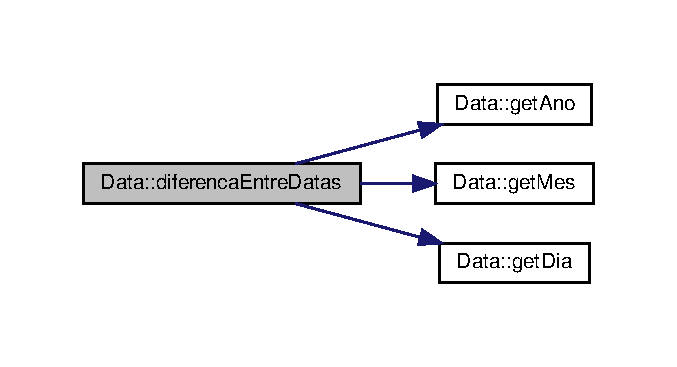
\includegraphics[width=325pt]{classData_a495d15dd0d90b595740f6e09fd0a2177_cgraph}
\end{center}
\end{figure}
Here is the caller graph for this function\+:
\nopagebreak
\begin{figure}[H]
\begin{center}
\leavevmode
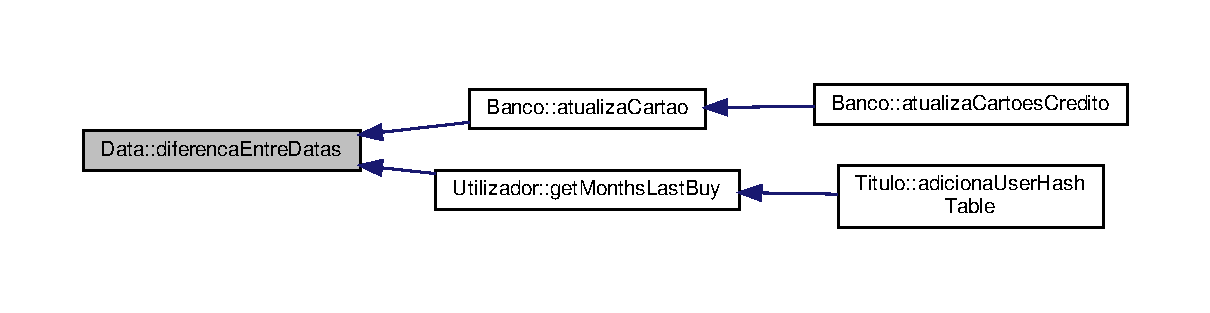
\includegraphics[width=350pt]{classData_a495d15dd0d90b595740f6e09fd0a2177_icgraph}
\end{center}
\end{figure}
\mbox{\Hypertarget{classData_ae19e0d5af87f94f2809ba52dae69e15b}\label{classData_ae19e0d5af87f94f2809ba52dae69e15b}} 
\index{Data@{Data}!get\+Ano@{get\+Ano}}
\index{get\+Ano@{get\+Ano}!Data@{Data}}
\subsubsection{\texorpdfstring{get\+Ano()}{getAno()}}
{\footnotesize\ttfamily unsigned int Data\+::get\+Ano (\begin{DoxyParamCaption}{ }\end{DoxyParamCaption}) const}



Devolve o ano. 

\begin{DoxyReturn}{Returns}
Retorna o ano da data 
\end{DoxyReturn}

\begin{DoxyCode}
49                                 \{
50     \textcolor{keywordflow}{return} ano;
51 \}
\end{DoxyCode}
Here is the caller graph for this function\+:
\nopagebreak
\begin{figure}[H]
\begin{center}
\leavevmode
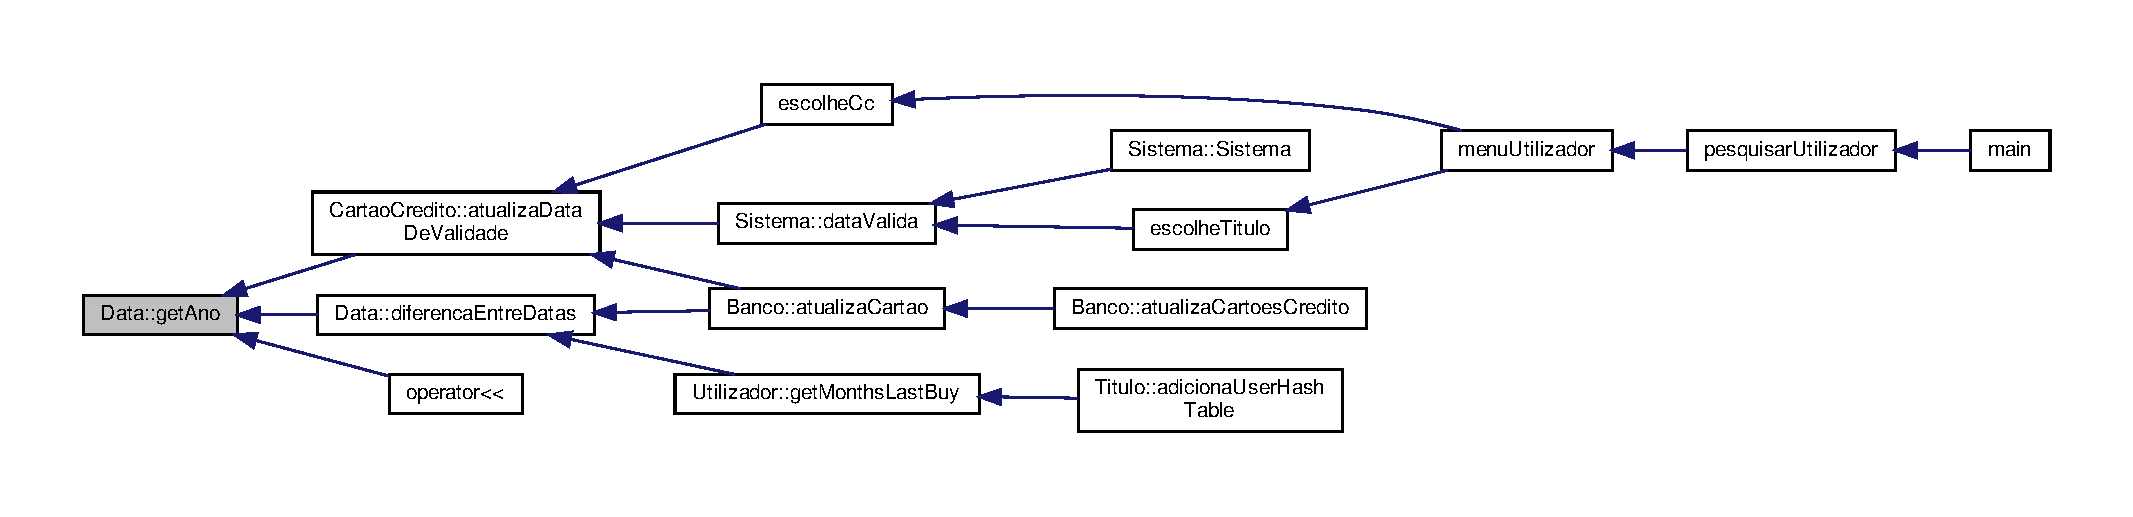
\includegraphics[width=350pt]{classData_ae19e0d5af87f94f2809ba52dae69e15b_icgraph}
\end{center}
\end{figure}
\mbox{\Hypertarget{classData_a459536c9351759b5697ba25456d9bd70}\label{classData_a459536c9351759b5697ba25456d9bd70}} 
\index{Data@{Data}!get\+Dia@{get\+Dia}}
\index{get\+Dia@{get\+Dia}!Data@{Data}}
\subsubsection{\texorpdfstring{get\+Dia()}{getDia()}}
{\footnotesize\ttfamily unsigned int Data\+::get\+Dia (\begin{DoxyParamCaption}{ }\end{DoxyParamCaption}) const}



Devolve o dia. 

\begin{DoxyReturn}{Returns}
Retorna o dia da data 
\end{DoxyReturn}

\begin{DoxyCode}
41                                 \{
42     \textcolor{keywordflow}{return} dia;
43 \}
\end{DoxyCode}
Here is the caller graph for this function\+:
\nopagebreak
\begin{figure}[H]
\begin{center}
\leavevmode
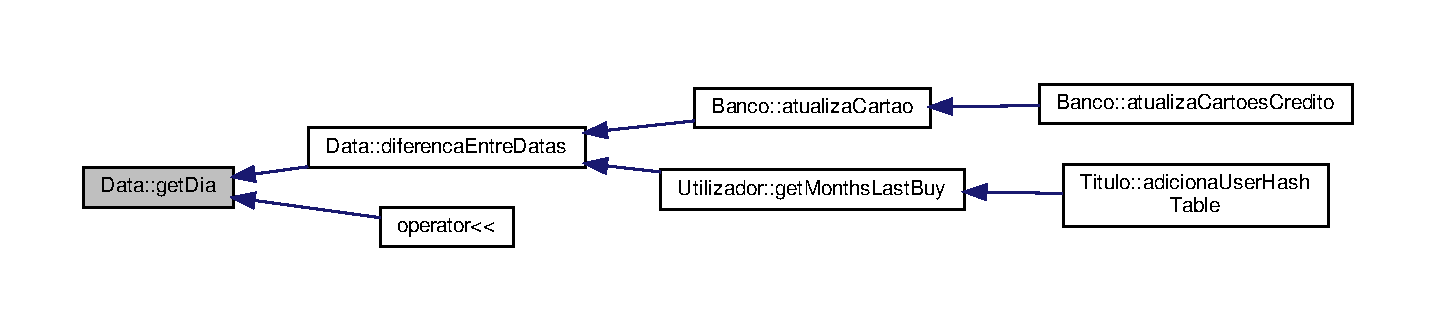
\includegraphics[width=350pt]{classData_a459536c9351759b5697ba25456d9bd70_icgraph}
\end{center}
\end{figure}
\mbox{\Hypertarget{classData_ab991d6a069c799930899b39bef9a4662}\label{classData_ab991d6a069c799930899b39bef9a4662}} 
\index{Data@{Data}!get\+Mes@{get\+Mes}}
\index{get\+Mes@{get\+Mes}!Data@{Data}}
\subsubsection{\texorpdfstring{get\+Mes()}{getMes()}}
{\footnotesize\ttfamily unsigned int Data\+::get\+Mes (\begin{DoxyParamCaption}{ }\end{DoxyParamCaption}) const}



Devolve o mes. 

\begin{DoxyReturn}{Returns}
Retorna o mes da data 
\end{DoxyReturn}

\begin{DoxyCode}
45                                 \{
46     \textcolor{keywordflow}{return} mes;
47 \}
\end{DoxyCode}
Here is the caller graph for this function\+:
\nopagebreak
\begin{figure}[H]
\begin{center}
\leavevmode
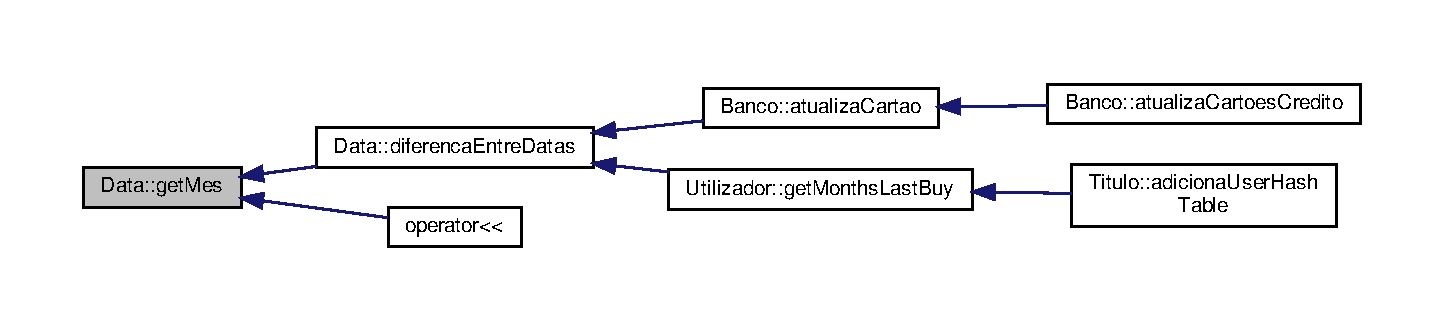
\includegraphics[width=350pt]{classData_ab991d6a069c799930899b39bef9a4662_icgraph}
\end{center}
\end{figure}
\mbox{\Hypertarget{classData_a28b51c511a389cf30b9d1d2da858f3f6}\label{classData_a28b51c511a389cf30b9d1d2da858f3f6}} 
\index{Data@{Data}!operator$<$@{operator$<$}}
\index{operator$<$@{operator$<$}!Data@{Data}}
\subsubsection{\texorpdfstring{operator$<$()}{operator<()}}
{\footnotesize\ttfamily bool Data\+::operator$<$ (\begin{DoxyParamCaption}\item[{const \hyperlink{classData}{Data} \&}]{D1 }\end{DoxyParamCaption}) const}



Overload do operador $<$ que compara duas data. 


\begin{DoxyParams}{Parameters}
{\em D1} & -\/ data com que se compara o objeto atual \\
\hline
\end{DoxyParams}
\begin{DoxyReturn}{Returns}
verdade se o objeto for menor que D1 
\end{DoxyReturn}

\begin{DoxyCode}
93                                          \{
94 
95     \textcolor{keywordflow}{if} (ano > D1.ano)
96         \textcolor{keywordflow}{return} \textcolor{keyword}{false};
97     \textcolor{keywordflow}{else} \textcolor{keywordflow}{if} (ano == D1.ano) \{
98 
99         \textcolor{keywordflow}{if} (mes > D1.mes)
100             \textcolor{keywordflow}{return} \textcolor{keyword}{false};
101         \textcolor{keywordflow}{else} \textcolor{keywordflow}{if}(mes==D1.mes)\{
102             \textcolor{keywordflow}{if} (dia >= D1.mes)
103                 \textcolor{keywordflow}{return} \textcolor{keyword}{false};
104         \}
105 
106         \textcolor{keywordflow}{return} \textcolor{keyword}{true};
107     \} \textcolor{keywordflow}{else}
108         \textcolor{keywordflow}{return} \textcolor{keyword}{true};
109 \}
\end{DoxyCode}
\mbox{\Hypertarget{classData_a8c3fdab05b3e81bb7b302b1d4d9a9d1f}\label{classData_a8c3fdab05b3e81bb7b302b1d4d9a9d1f}} 
\index{Data@{Data}!operator$<$=@{operator$<$=}}
\index{operator$<$=@{operator$<$=}!Data@{Data}}
\subsubsection{\texorpdfstring{operator$<$=()}{operator<=()}}
{\footnotesize\ttfamily bool Data\+::operator$<$= (\begin{DoxyParamCaption}\item[{const \hyperlink{classData}{Data} \&}]{D1 }\end{DoxyParamCaption}) const}



Overload do operador $<$= que compara duas data. 


\begin{DoxyParams}{Parameters}
{\em D1} & -\/ data com que se compara o objeto atual \\
\hline
\end{DoxyParams}
\begin{DoxyReturn}{Returns}
verdade se o objeto for menor ou igual que D1 
\end{DoxyReturn}

\begin{DoxyCode}
77                                           \{
78 
79     \textcolor{keywordflow}{if} (ano > D1.ano)
80         \textcolor{keywordflow}{return} \textcolor{keyword}{false};
81     \textcolor{keywordflow}{else} \textcolor{keywordflow}{if} (ano == D1.ano) \{
82 
83         \textcolor{keywordflow}{if} (mes > D1.mes)
84             \textcolor{keywordflow}{return} \textcolor{keyword}{false};
85         \textcolor{keywordflow}{if} (dia > D1.mes)
86             \textcolor{keywordflow}{return} \textcolor{keyword}{false};
87 
88         \textcolor{keywordflow}{return} \textcolor{keyword}{true};
89     \} \textcolor{keywordflow}{else}
90         \textcolor{keywordflow}{return} \textcolor{keyword}{true};
91 \}
\end{DoxyCode}
\mbox{\Hypertarget{classData_af00bf4efbd3504689f6bc7283378ba5f}\label{classData_af00bf4efbd3504689f6bc7283378ba5f}} 
\index{Data@{Data}!operator==@{operator==}}
\index{operator==@{operator==}!Data@{Data}}
\subsubsection{\texorpdfstring{operator==()}{operator==()}}
{\footnotesize\ttfamily bool Data\+::operator== (\begin{DoxyParamCaption}\item[{const \hyperlink{classData}{Data} \&}]{D1 }\end{DoxyParamCaption}) const}



overload do operador == que compara duas data 


\begin{DoxyParams}{Parameters}
{\em D1} & -\/ data com que se compara o objeto atual \\
\hline
\end{DoxyParams}
\begin{DoxyReturn}{Returns}
Retorna verdade se forem iguais 
\end{DoxyReturn}

\begin{DoxyCode}
111                                             \{
112     \textcolor{keywordflow}{return} (this->ano == D2.ano) && (this->mes == D2.mes)
113             && (this->dia == D2.dia);
114 \}
\end{DoxyCode}
\mbox{\Hypertarget{classData_a8d4cfad647b590df436d8260000a2745}\label{classData_a8d4cfad647b590df436d8260000a2745}} 
\index{Data@{Data}!set\+Ano@{set\+Ano}}
\index{set\+Ano@{set\+Ano}!Data@{Data}}
\subsubsection{\texorpdfstring{set\+Ano()}{setAno()}}
{\footnotesize\ttfamily \hyperlink{classData}{Data} \& Data\+::set\+Ano (\begin{DoxyParamCaption}\item[{const unsigned int}]{ano }\end{DoxyParamCaption})}



Altera o dia. 


\begin{DoxyParams}{Parameters}
{\em ano} & -\/ Valor a aplicar a ano \\
\hline
\end{DoxyParams}
\begin{DoxyReturn}{Returns}
Retorna referencia para \hyperlink{classData}{Data} para fazer chamadas de funcao em sequencia 
\end{DoxyReturn}

\begin{DoxyCode}
36                                           \{
37     this->ano = ano;
38     \textcolor{keywordflow}{return} *\textcolor{keyword}{this};
39 \}
\end{DoxyCode}
Here is the caller graph for this function\+:
\nopagebreak
\begin{figure}[H]
\begin{center}
\leavevmode
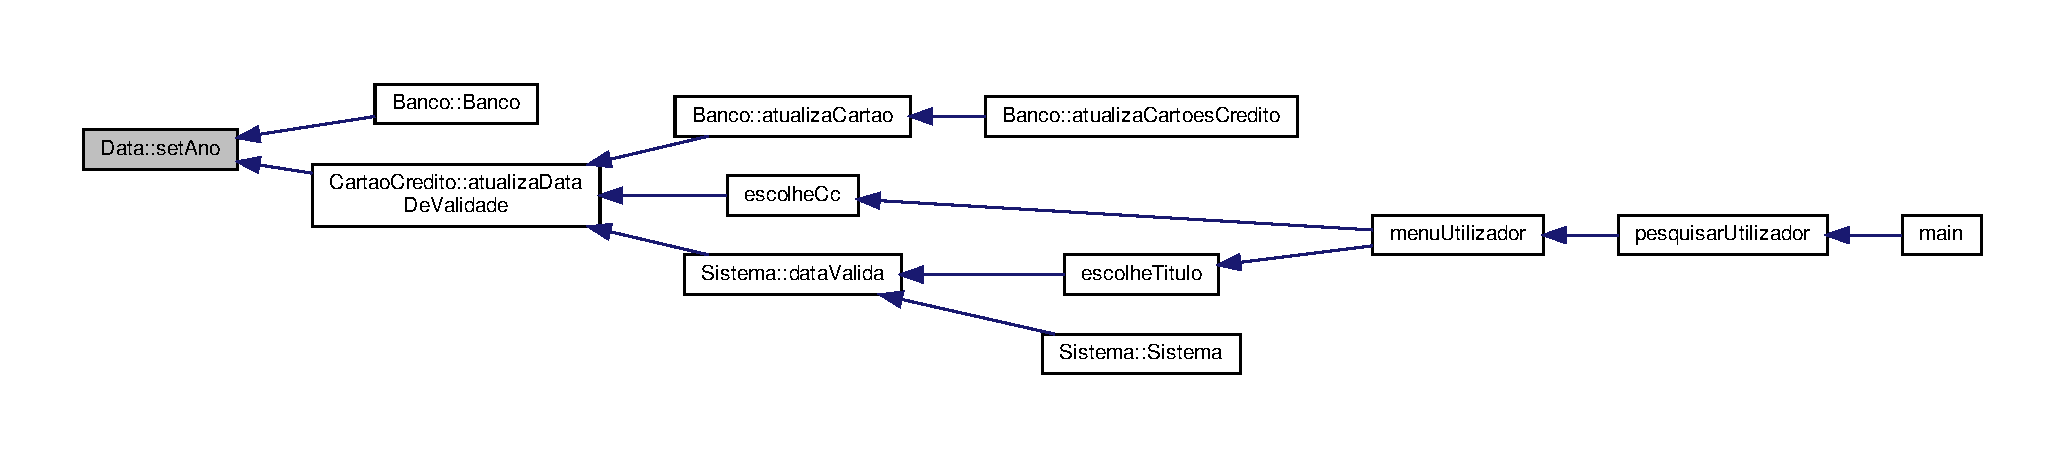
\includegraphics[width=350pt]{classData_a8d4cfad647b590df436d8260000a2745_icgraph}
\end{center}
\end{figure}
\mbox{\Hypertarget{classData_a3e2c5356bc8d548b75c7d085f7a7c4ee}\label{classData_a3e2c5356bc8d548b75c7d085f7a7c4ee}} 
\index{Data@{Data}!set\+Dia@{set\+Dia}}
\index{set\+Dia@{set\+Dia}!Data@{Data}}
\subsubsection{\texorpdfstring{set\+Dia()}{setDia()}}
{\footnotesize\ttfamily \hyperlink{classData}{Data} \& Data\+::set\+Dia (\begin{DoxyParamCaption}\item[{const unsigned int}]{dia }\end{DoxyParamCaption})}



Altera o dia. 


\begin{DoxyParams}{Parameters}
{\em dia} & -\/ Valor a aplicar a dia \\
\hline
\end{DoxyParams}
\begin{DoxyReturn}{Returns}
Retorna referencia para \hyperlink{classData}{Data} para fazer chamadas de funcao em sequencia 
\end{DoxyReturn}

\begin{DoxyCode}
26                                           \{
27     this->dia = dia;
28     \textcolor{keywordflow}{return} *\textcolor{keyword}{this};
29 \}
\end{DoxyCode}
Here is the caller graph for this function\+:
\nopagebreak
\begin{figure}[H]
\begin{center}
\leavevmode
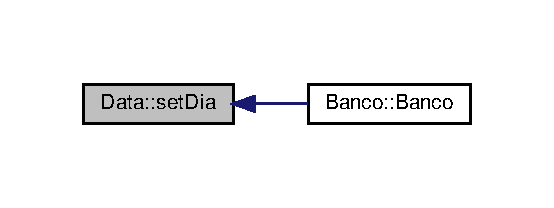
\includegraphics[width=266pt]{classData_a3e2c5356bc8d548b75c7d085f7a7c4ee_icgraph}
\end{center}
\end{figure}
\mbox{\Hypertarget{classData_ab15051ae481d89d057b22abc8152584c}\label{classData_ab15051ae481d89d057b22abc8152584c}} 
\index{Data@{Data}!set\+Mes@{set\+Mes}}
\index{set\+Mes@{set\+Mes}!Data@{Data}}
\subsubsection{\texorpdfstring{set\+Mes()}{setMes()}}
{\footnotesize\ttfamily \hyperlink{classData}{Data} \& Data\+::set\+Mes (\begin{DoxyParamCaption}\item[{const unsigned int}]{mes }\end{DoxyParamCaption})}



Altera o mes. 


\begin{DoxyParams}{Parameters}
{\em mes} & -\/ Valor a aplicar ao mes \\
\hline
\end{DoxyParams}
\begin{DoxyReturn}{Returns}
Retorna referencia para \hyperlink{classData}{Data} para fazer chamadas de funcao em sequencia 
\end{DoxyReturn}

\begin{DoxyCode}
31                                           \{
32     this->mes = mes;
33     \textcolor{keywordflow}{return} *\textcolor{keyword}{this};
34 \}
\end{DoxyCode}
Here is the caller graph for this function\+:
\nopagebreak
\begin{figure}[H]
\begin{center}
\leavevmode
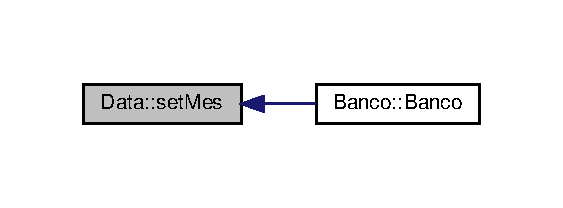
\includegraphics[width=270pt]{classData_ab15051ae481d89d057b22abc8152584c_icgraph}
\end{center}
\end{figure}


The documentation for this class was generated from the following files\+:\begin{DoxyCompactItemize}
\item 
\hyperlink{Data_8h}{Data.\+h}\item 
\hyperlink{Data_8cpp}{Data.\+cpp}\end{DoxyCompactItemize}

\hypertarget{classDataInvalida}{}\section{Data\+Invalida Class Reference}
\label{classDataInvalida}\index{Data\+Invalida@{Data\+Invalida}}


{\ttfamily \#include $<$Erro.\+h$>$}



Inheritance diagram for Data\+Invalida\+:
\nopagebreak
\begin{figure}[H]
\begin{center}
\leavevmode
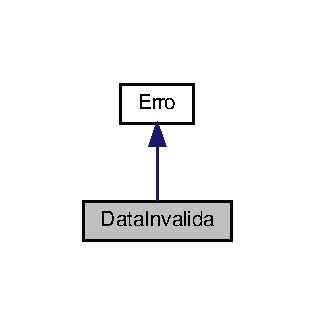
\includegraphics[width=151pt]{classDataInvalida__inherit__graph}
\end{center}
\end{figure}


Collaboration diagram for Data\+Invalida\+:
\nopagebreak
\begin{figure}[H]
\begin{center}
\leavevmode
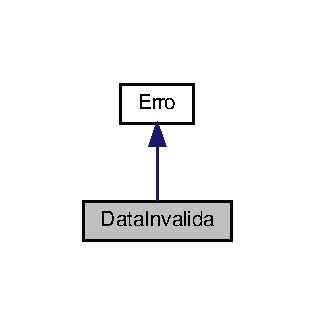
\includegraphics[width=151pt]{classDataInvalida__coll__graph}
\end{center}
\end{figure}
\subsection*{Public Member Functions}
\begin{DoxyCompactItemize}
\item 
\hyperlink{classDataInvalida_af024b53b8f0ba3c388a6283df30d7123}{Data\+Invalida} (const std\+::string \&info)
\begin{DoxyCompactList}\small\item\em Construtor da classe \hyperlink{classDataInvalida}{Data\+Invalida}. \end{DoxyCompactList}\end{DoxyCompactItemize}


\subsection{Detailed Description}
Classe utilizada para lancar excecoes do tipo \hyperlink{classData}{Data} Invalida 

\subsection{Constructor \& Destructor Documentation}
\mbox{\Hypertarget{classDataInvalida_af024b53b8f0ba3c388a6283df30d7123}\label{classDataInvalida_af024b53b8f0ba3c388a6283df30d7123}} 
\index{Data\+Invalida@{Data\+Invalida}!Data\+Invalida@{Data\+Invalida}}
\index{Data\+Invalida@{Data\+Invalida}!Data\+Invalida@{Data\+Invalida}}
\subsubsection{\texorpdfstring{Data\+Invalida()}{DataInvalida()}}
{\footnotesize\ttfamily Data\+Invalida\+::\+Data\+Invalida (\begin{DoxyParamCaption}\item[{const std\+::string \&}]{info }\end{DoxyParamCaption})\hspace{0.3cm}{\ttfamily [inline]}}



Construtor da classe \hyperlink{classDataInvalida}{Data\+Invalida}. 


\begin{DoxyCode}
37 : \hyperlink{classErro_a15d79796bd17517ff05d45eee55556f1}{Erro}(info) \{ \}
\end{DoxyCode}


The documentation for this class was generated from the following file\+:\begin{DoxyCompactItemize}
\item 
\hyperlink{Erro_8h}{Erro.\+h}\end{DoxyCompactItemize}

\hypertarget{classEmpresa}{}\section{Empresa Class Reference}
\label{classEmpresa}\index{Empresa@{Empresa}}


{\ttfamily \#include $<$Empresa.\+h$>$}

\subsection*{Public Member Functions}
\begin{DoxyCompactItemize}
\item 
\hyperlink{classEmpresa_aff124b958356c479ab50ddf4cf302193}{Empresa} ()
\begin{DoxyCompactList}\small\item\em Construtor por default da classe empresa. \end{DoxyCompactList}\item 
\hyperlink{classEmpresa_a19748f9e5c99292e3cd1489712751271}{Empresa} (std\+::string nome, std\+::string email, std\+::string numero\+Telemovel, std\+::string nif)
\begin{DoxyCompactList}\small\item\em Construtor da classe empresa. \end{DoxyCompactList}\item 
void \hyperlink{classEmpresa_a3c6eb96c694dcb6db1e402d6db1c439a}{criar\+Titulo} (\hyperlink{classTitulo}{Titulo} $\ast$t)
\begin{DoxyCompactList}\small\item\em Adiciona um titulo novo a empresa. \end{DoxyCompactList}\item 
std\+::string \hyperlink{classEmpresa_a99bc2de98a0c0348abb74c93e6e7159e}{get\+Nome\+Empresa} () const
\begin{DoxyCompactList}\small\item\em Devolve o nome da empresa. \end{DoxyCompactList}\item 
unsigned int \hyperlink{classEmpresa_a49b2b94a54bbc341822f64fc194f98fd}{get\+Numero\+Titulos} () const
\begin{DoxyCompactList}\small\item\em Devolve o numero de titulos da empresa. \end{DoxyCompactList}\item 
std\+::string \hyperlink{classEmpresa_a6ab12452496ccaea5493bd2c67824f09}{get\+Nif} () const
\begin{DoxyCompactList}\small\item\em Devolve o N\+IF da empresa. \end{DoxyCompactList}\item 
\hyperlink{structcontactos}{contactos} \hyperlink{classEmpresa_a19396f860d9b17f94bd262ba093d76eb}{get\+Contactos} () const
\begin{DoxyCompactList}\small\item\em Devolve os contactos da empresa. \end{DoxyCompactList}\item 
std\+::vector$<$ \hyperlink{classTitulo}{Titulo} $\ast$ $>$ \hyperlink{classEmpresa_a672f3a89b0e41dd758ab6baf1a8dfbd2}{get\+Titulos} () const
\begin{DoxyCompactList}\small\item\em Devolve os titulos da empresa. \end{DoxyCompactList}\item 
void \hyperlink{classEmpresa_af067f4d00a5ceb8816a607164916d2e1}{display\+Titulos} ()
\begin{DoxyCompactList}\small\item\em Mostra os titulos da empresa no ecra. \end{DoxyCompactList}\item 
void \hyperlink{classEmpresa_a3e40c710d76874bcfcf4bd83592d4f13}{add\+Numero} ()
\begin{DoxyCompactList}\small\item\em Incrementa o numero de titulos da empresa. \end{DoxyCompactList}\item 
bool \hyperlink{classEmpresa_ab643d752365e59fa1d90a41b8a036d6a}{operator$<$} (const \hyperlink{classEmpresa}{Empresa} \&empresa)
\begin{DoxyCompactList}\small\item\em Overload do operador menor para objetos da classe \hyperlink{classEmpresa}{Empresa}. \end{DoxyCompactList}\item 
bool \hyperlink{classEmpresa_ad915fb38bc6c73c02fe70c62db1c9f03}{operator==} (const \hyperlink{classEmpresa}{Empresa} \&empresa)
\begin{DoxyCompactList}\small\item\em Overload do operador igual para objetos da classe \hyperlink{classEmpresa}{Empresa}. \end{DoxyCompactList}\end{DoxyCompactItemize}


\subsection{Constructor \& Destructor Documentation}
\mbox{\Hypertarget{classEmpresa_aff124b958356c479ab50ddf4cf302193}\label{classEmpresa_aff124b958356c479ab50ddf4cf302193}} 
\index{Empresa@{Empresa}!Empresa@{Empresa}}
\index{Empresa@{Empresa}!Empresa@{Empresa}}
\subsubsection{\texorpdfstring{Empresa()}{Empresa()}\hspace{0.1cm}{\footnotesize\ttfamily [1/2]}}
{\footnotesize\ttfamily Empresa\+::\+Empresa (\begin{DoxyParamCaption}{ }\end{DoxyParamCaption})\hspace{0.3cm}{\ttfamily [inline]}}



Construtor por default da classe empresa. 


\begin{DoxyCode}
26 \{this->numeroTitulos=0;\}
\end{DoxyCode}
Here is the call graph for this function\+:
\nopagebreak
\begin{figure}[H]
\begin{center}
\leavevmode
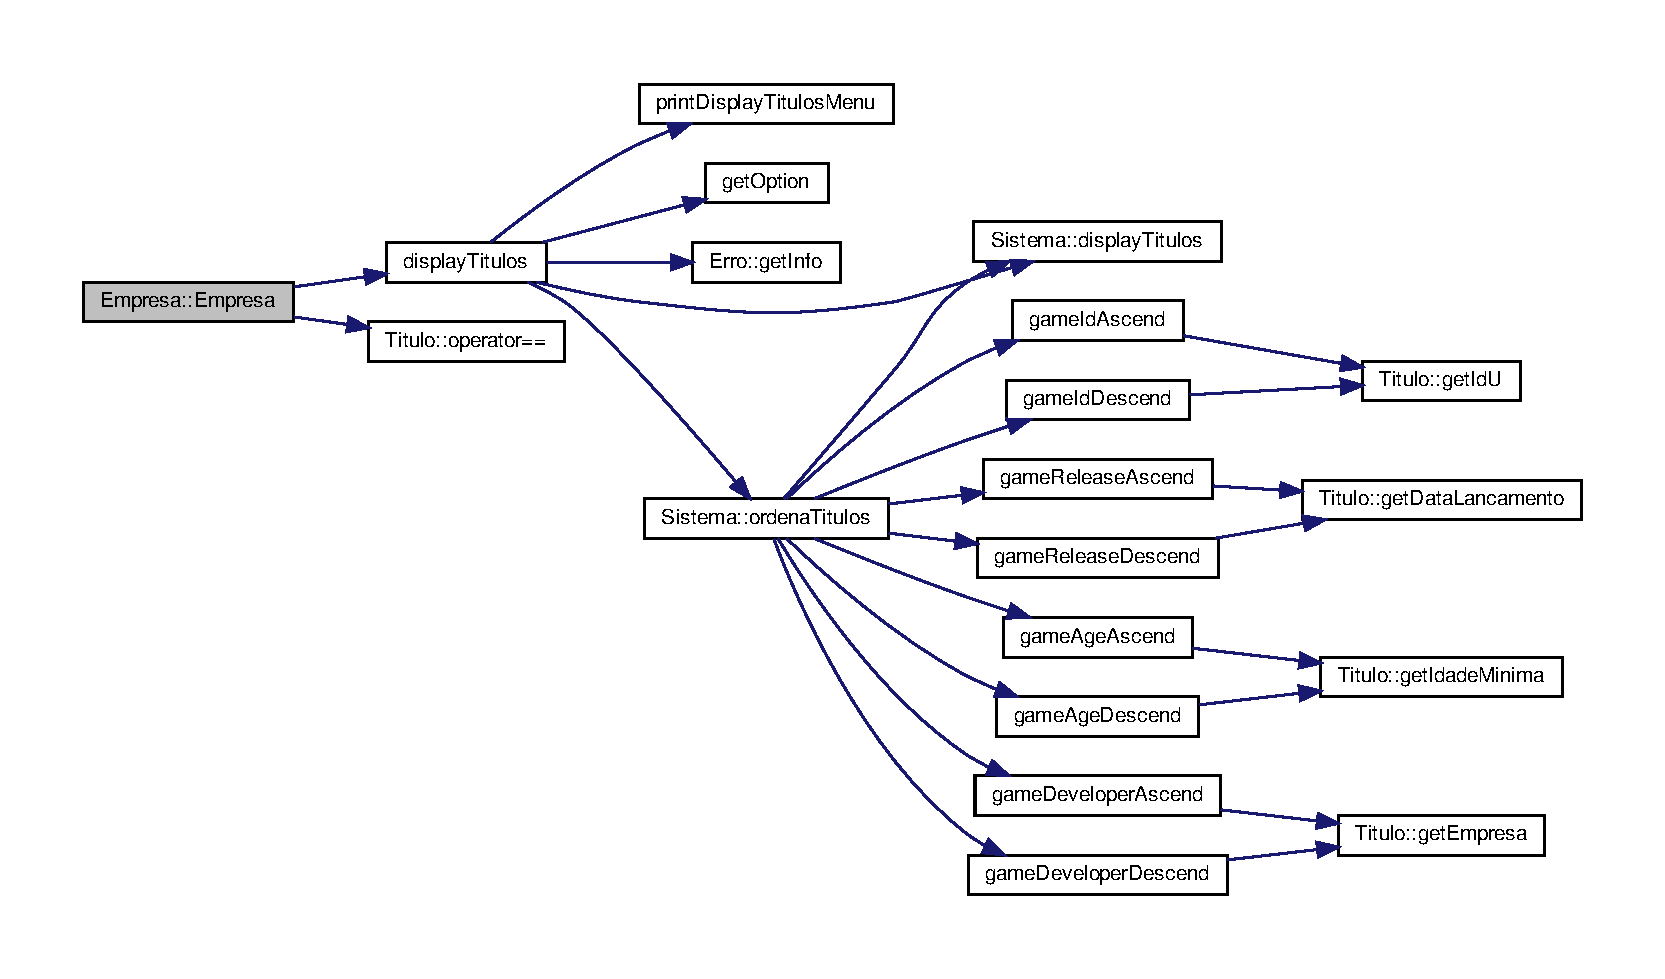
\includegraphics[width=350pt]{classEmpresa_aff124b958356c479ab50ddf4cf302193_cgraph}
\end{center}
\end{figure}
\mbox{\Hypertarget{classEmpresa_a19748f9e5c99292e3cd1489712751271}\label{classEmpresa_a19748f9e5c99292e3cd1489712751271}} 
\index{Empresa@{Empresa}!Empresa@{Empresa}}
\index{Empresa@{Empresa}!Empresa@{Empresa}}
\subsubsection{\texorpdfstring{Empresa()}{Empresa()}\hspace{0.1cm}{\footnotesize\ttfamily [2/2]}}
{\footnotesize\ttfamily Empresa\+::\+Empresa (\begin{DoxyParamCaption}\item[{std\+::string}]{nome,  }\item[{std\+::string}]{email,  }\item[{std\+::string}]{numero\+Telemovel,  }\item[{std\+::string}]{nif }\end{DoxyParamCaption})}



Construtor da classe empresa. 


\begin{DoxyParams}{Parameters}
{\em nome} & -\/ nome da empresa \\
\hline
{\em email} & -\/ email da empresa \\
\hline
{\em numero\+Telemovel} & -\/ numero de telemovel da empresa \\
\hline
{\em nif} & -\/ nif da empresa \\
\hline
\end{DoxyParams}

\begin{DoxyCode}
6      :nome(nome),Nif(nif) \{
7 
8     this->numeroTitulos=0;
9     this->contacto.\hyperlink{structcontactos_a86c1ad3bcc23dbb8bf7bb37ae0976242}{email}=email;
10     this->contacto.\hyperlink{structcontactos_a09e1d4029e1eb91fc9ec76e4b4b6d48a}{numeroTelemovel}=numeroTelemovel;
11 
12 \}
\end{DoxyCode}


\subsection{Member Function Documentation}
\mbox{\Hypertarget{classEmpresa_a3e40c710d76874bcfcf4bd83592d4f13}\label{classEmpresa_a3e40c710d76874bcfcf4bd83592d4f13}} 
\index{Empresa@{Empresa}!add\+Numero@{add\+Numero}}
\index{add\+Numero@{add\+Numero}!Empresa@{Empresa}}
\subsubsection{\texorpdfstring{add\+Numero()}{addNumero()}}
{\footnotesize\ttfamily void Empresa\+::add\+Numero (\begin{DoxyParamCaption}{ }\end{DoxyParamCaption})}



Incrementa o numero de titulos da empresa. 


\begin{DoxyCode}
34                         \{
35     this->numeroTitulos++;
36 \}
\end{DoxyCode}
\mbox{\Hypertarget{classEmpresa_a3c6eb96c694dcb6db1e402d6db1c439a}\label{classEmpresa_a3c6eb96c694dcb6db1e402d6db1c439a}} 
\index{Empresa@{Empresa}!criar\+Titulo@{criar\+Titulo}}
\index{criar\+Titulo@{criar\+Titulo}!Empresa@{Empresa}}
\subsubsection{\texorpdfstring{criar\+Titulo()}{criarTitulo()}}
{\footnotesize\ttfamily void Empresa\+::criar\+Titulo (\begin{DoxyParamCaption}\item[{\hyperlink{classTitulo}{Titulo} $\ast$}]{t }\end{DoxyParamCaption})}



Adiciona um titulo novo a empresa. 


\begin{DoxyCode}
50                                     \{
51 
52     \textcolor{keywordflow}{for}(\textcolor{keyword}{const} \textcolor{keyword}{auto} & titles : this->Titulos) \{
53         \textcolor{keywordflow}{if}(titles==t)
54             \textcolor{keywordflow}{return};\textcolor{comment}{//throw(EmpresaJaComTitulo(t))}
55     \}
56     this->numeroTitulos++;
57     this->Titulos.push\_back(t);
58 \}
\end{DoxyCode}
Here is the caller graph for this function\+:
\nopagebreak
\begin{figure}[H]
\begin{center}
\leavevmode
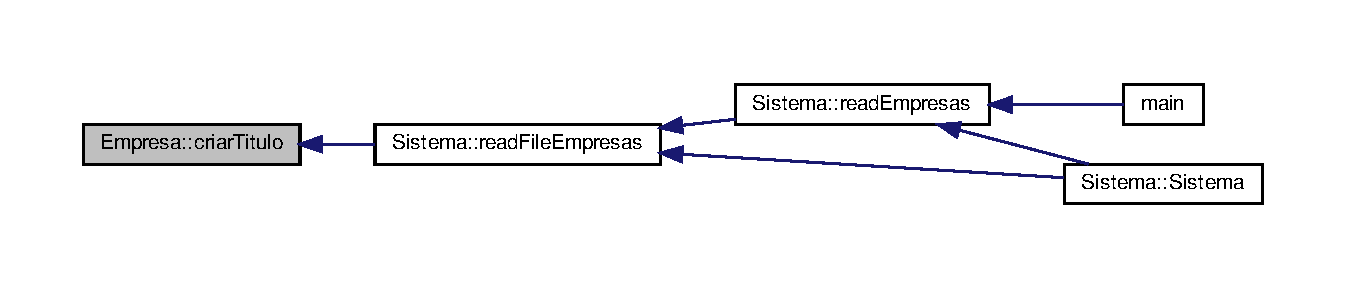
\includegraphics[width=350pt]{classEmpresa_a3c6eb96c694dcb6db1e402d6db1c439a_icgraph}
\end{center}
\end{figure}
\mbox{\Hypertarget{classEmpresa_af067f4d00a5ceb8816a607164916d2e1}\label{classEmpresa_af067f4d00a5ceb8816a607164916d2e1}} 
\index{Empresa@{Empresa}!display\+Titulos@{display\+Titulos}}
\index{display\+Titulos@{display\+Titulos}!Empresa@{Empresa}}
\subsubsection{\texorpdfstring{display\+Titulos()}{displayTitulos()}}
{\footnotesize\ttfamily void Empresa\+::display\+Titulos (\begin{DoxyParamCaption}{ }\end{DoxyParamCaption})}



Mostra os titulos da empresa no ecra. 


\begin{DoxyCode}
60                              \{
61 
62     \textcolor{keywordflow}{for}(\textcolor{keyword}{const} \textcolor{keyword}{auto} & titulo : this->Titulos) \{
63         std::cout << titulo->getNome() << \textcolor{stringliteral}{", "} << titulo->getEmpresa() << \textcolor{stringliteral}{", "} << titulo->getPlataforma() <
      < \textcolor{stringliteral}{", "} << titulo->getPreco() << \textcolor{stringliteral}{" euros, (desconto: "} << titulo->getDesconto() << \textcolor{stringliteral}{"% ), "} << titulo->
      getDataLancamento().getAno() << \textcolor{stringliteral}{", idade minima: "} << titulo->getIdadeMinima() << std::endl;
64     \}
65 \}
\end{DoxyCode}
Here is the caller graph for this function\+:
\nopagebreak
\begin{figure}[H]
\begin{center}
\leavevmode
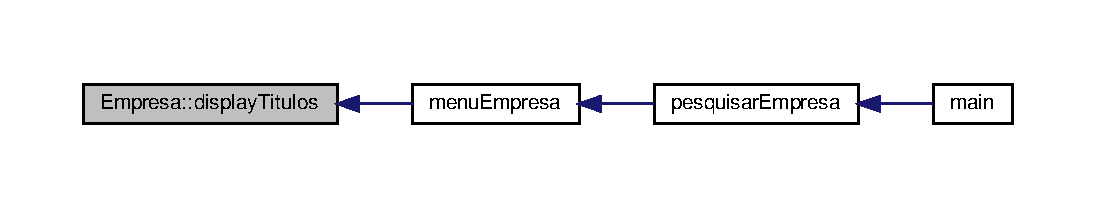
\includegraphics[width=350pt]{classEmpresa_af067f4d00a5ceb8816a607164916d2e1_icgraph}
\end{center}
\end{figure}
\mbox{\Hypertarget{classEmpresa_a19396f860d9b17f94bd262ba093d76eb}\label{classEmpresa_a19396f860d9b17f94bd262ba093d76eb}} 
\index{Empresa@{Empresa}!get\+Contactos@{get\+Contactos}}
\index{get\+Contactos@{get\+Contactos}!Empresa@{Empresa}}
\subsubsection{\texorpdfstring{get\+Contactos()}{getContactos()}}
{\footnotesize\ttfamily \hyperlink{structcontactos}{contactos} Empresa\+::get\+Contactos (\begin{DoxyParamCaption}{ }\end{DoxyParamCaption}) const}



Devolve os contactos da empresa. 

\begin{DoxyReturn}{Returns}
Retorna a struct contactos, da empresa 
\end{DoxyReturn}

\begin{DoxyCode}
26                                      \{
27     \textcolor{keywordflow}{return} this->contacto;
28 \}
\end{DoxyCode}
Here is the caller graph for this function\+:
\nopagebreak
\begin{figure}[H]
\begin{center}
\leavevmode
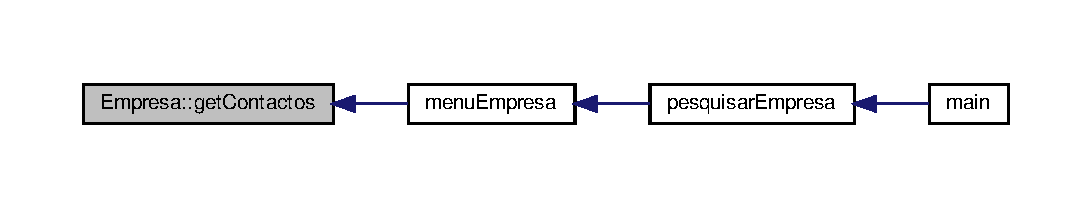
\includegraphics[width=350pt]{classEmpresa_a19396f860d9b17f94bd262ba093d76eb_icgraph}
\end{center}
\end{figure}
\mbox{\Hypertarget{classEmpresa_a6ab12452496ccaea5493bd2c67824f09}\label{classEmpresa_a6ab12452496ccaea5493bd2c67824f09}} 
\index{Empresa@{Empresa}!get\+Nif@{get\+Nif}}
\index{get\+Nif@{get\+Nif}!Empresa@{Empresa}}
\subsubsection{\texorpdfstring{get\+Nif()}{getNif()}}
{\footnotesize\ttfamily std\+::string Empresa\+::get\+Nif (\begin{DoxyParamCaption}{ }\end{DoxyParamCaption}) const}



Devolve o N\+IF da empresa. 

\begin{DoxyReturn}{Returns}
retorna o N\+IF da empresa 
\end{DoxyReturn}

\begin{DoxyCode}
22                                \{
23     \textcolor{keywordflow}{return} this->Nif;
24 \}
\end{DoxyCode}
Here is the caller graph for this function\+:
\nopagebreak
\begin{figure}[H]
\begin{center}
\leavevmode
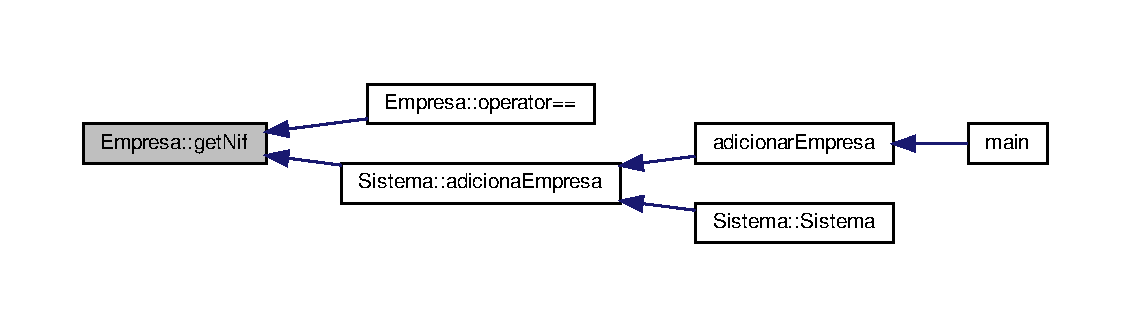
\includegraphics[width=350pt]{classEmpresa_a6ab12452496ccaea5493bd2c67824f09_icgraph}
\end{center}
\end{figure}
\mbox{\Hypertarget{classEmpresa_a99bc2de98a0c0348abb74c93e6e7159e}\label{classEmpresa_a99bc2de98a0c0348abb74c93e6e7159e}} 
\index{Empresa@{Empresa}!get\+Nome\+Empresa@{get\+Nome\+Empresa}}
\index{get\+Nome\+Empresa@{get\+Nome\+Empresa}!Empresa@{Empresa}}
\subsubsection{\texorpdfstring{get\+Nome\+Empresa()}{getNomeEmpresa()}}
{\footnotesize\ttfamily std\+::string Empresa\+::get\+Nome\+Empresa (\begin{DoxyParamCaption}{ }\end{DoxyParamCaption}) const}



Devolve o nome da empresa. 

\begin{DoxyReturn}{Returns}
Retorna o nome da empresa 
\end{DoxyReturn}

\begin{DoxyCode}
18                                        \{
19     \textcolor{keywordflow}{return} this->nome;
20 \}
\end{DoxyCode}
Here is the caller graph for this function\+:
\nopagebreak
\begin{figure}[H]
\begin{center}
\leavevmode
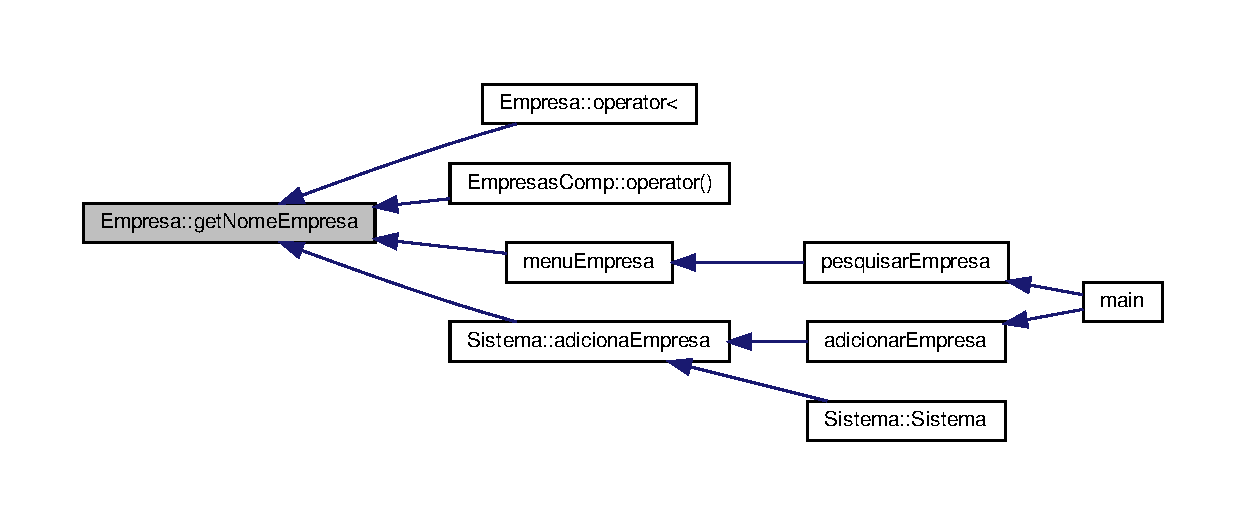
\includegraphics[width=350pt]{classEmpresa_a99bc2de98a0c0348abb74c93e6e7159e_icgraph}
\end{center}
\end{figure}
\mbox{\Hypertarget{classEmpresa_a49b2b94a54bbc341822f64fc194f98fd}\label{classEmpresa_a49b2b94a54bbc341822f64fc194f98fd}} 
\index{Empresa@{Empresa}!get\+Numero\+Titulos@{get\+Numero\+Titulos}}
\index{get\+Numero\+Titulos@{get\+Numero\+Titulos}!Empresa@{Empresa}}
\subsubsection{\texorpdfstring{get\+Numero\+Titulos()}{getNumeroTitulos()}}
{\footnotesize\ttfamily unsigned int Empresa\+::get\+Numero\+Titulos (\begin{DoxyParamCaption}{ }\end{DoxyParamCaption}) const}



Devolve o numero de titulos da empresa. 

\begin{DoxyReturn}{Returns}
Retorna o numero de titulos da empresa 
\end{DoxyReturn}

\begin{DoxyCode}
14                                             \{
15     \textcolor{keywordflow}{return} this->numeroTitulos;
16 \}
\end{DoxyCode}
Here is the caller graph for this function\+:
\nopagebreak
\begin{figure}[H]
\begin{center}
\leavevmode
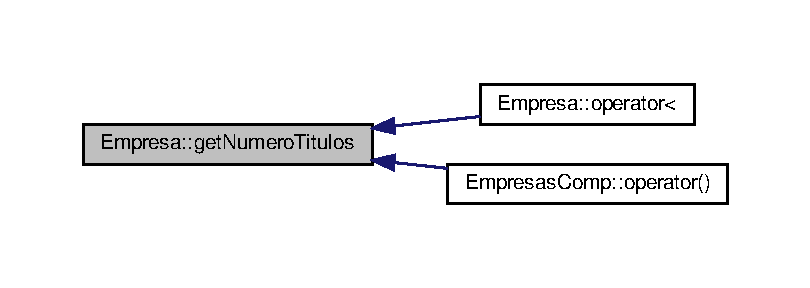
\includegraphics[width=350pt]{classEmpresa_a49b2b94a54bbc341822f64fc194f98fd_icgraph}
\end{center}
\end{figure}
\mbox{\Hypertarget{classEmpresa_a672f3a89b0e41dd758ab6baf1a8dfbd2}\label{classEmpresa_a672f3a89b0e41dd758ab6baf1a8dfbd2}} 
\index{Empresa@{Empresa}!get\+Titulos@{get\+Titulos}}
\index{get\+Titulos@{get\+Titulos}!Empresa@{Empresa}}
\subsubsection{\texorpdfstring{get\+Titulos()}{getTitulos()}}
{\footnotesize\ttfamily std\+::vector$<$ \hyperlink{classTitulo}{Titulo} $\ast$ $>$ Empresa\+::get\+Titulos (\begin{DoxyParamCaption}{ }\end{DoxyParamCaption}) const}



Devolve os titulos da empresa. 

\begin{DoxyReturn}{Returns}
Retorna o vector com os titulos da empresa 
\end{DoxyReturn}

\begin{DoxyCode}
30                                             \{
31     \textcolor{keywordflow}{return} this->Titulos;
32 \}
\end{DoxyCode}
\mbox{\Hypertarget{classEmpresa_ab643d752365e59fa1d90a41b8a036d6a}\label{classEmpresa_ab643d752365e59fa1d90a41b8a036d6a}} 
\index{Empresa@{Empresa}!operator$<$@{operator$<$}}
\index{operator$<$@{operator$<$}!Empresa@{Empresa}}
\subsubsection{\texorpdfstring{operator$<$()}{operator<()}}
{\footnotesize\ttfamily bool Empresa\+::operator$<$ (\begin{DoxyParamCaption}\item[{const \hyperlink{classEmpresa}{Empresa} \&}]{empresa }\end{DoxyParamCaption})}



Overload do operador menor para objetos da classe \hyperlink{classEmpresa}{Empresa}. 


\begin{DoxyCode}
38                                                 \{
39 
40     \textcolor{keywordflow}{if}(this->numeroTitulos==empresa.\hyperlink{classEmpresa_a49b2b94a54bbc341822f64fc194f98fd}{getNumeroTitulos}())
41         \textcolor{keywordflow}{return} this->nome < empresa.\hyperlink{classEmpresa_a99bc2de98a0c0348abb74c93e6e7159e}{getNomeEmpresa}();
42      \textcolor{keywordflow}{else}
43          \textcolor{keywordflow}{return} this->numeroTitulos< empresa.\hyperlink{classEmpresa_a49b2b94a54bbc341822f64fc194f98fd}{getNumeroTitulos}();
44 \}
\end{DoxyCode}
Here is the call graph for this function\+:
\nopagebreak
\begin{figure}[H]
\begin{center}
\leavevmode
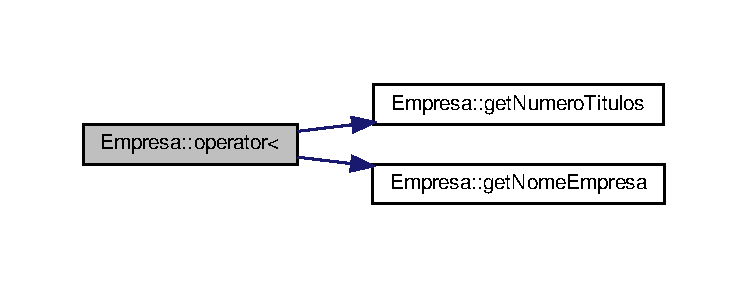
\includegraphics[width=350pt]{classEmpresa_ab643d752365e59fa1d90a41b8a036d6a_cgraph}
\end{center}
\end{figure}
\mbox{\Hypertarget{classEmpresa_ad915fb38bc6c73c02fe70c62db1c9f03}\label{classEmpresa_ad915fb38bc6c73c02fe70c62db1c9f03}} 
\index{Empresa@{Empresa}!operator==@{operator==}}
\index{operator==@{operator==}!Empresa@{Empresa}}
\subsubsection{\texorpdfstring{operator==()}{operator==()}}
{\footnotesize\ttfamily bool Empresa\+::operator== (\begin{DoxyParamCaption}\item[{const \hyperlink{classEmpresa}{Empresa} \&}]{empresa }\end{DoxyParamCaption})}



Overload do operador igual para objetos da classe \hyperlink{classEmpresa}{Empresa}. 


\begin{DoxyCode}
46                                                   \{
47     \textcolor{keywordflow}{return} this->Nif==empresa.\hyperlink{classEmpresa_a6ab12452496ccaea5493bd2c67824f09}{getNif}();
48 \}
\end{DoxyCode}
Here is the call graph for this function\+:
\nopagebreak
\begin{figure}[H]
\begin{center}
\leavevmode
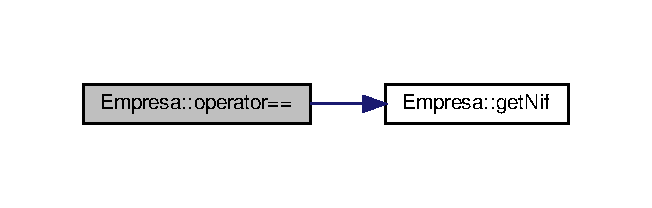
\includegraphics[width=313pt]{classEmpresa_ad915fb38bc6c73c02fe70c62db1c9f03_cgraph}
\end{center}
\end{figure}


The documentation for this class was generated from the following files\+:\begin{DoxyCompactItemize}
\item 
\hyperlink{Empresa_8h}{Empresa.\+h}\item 
\hyperlink{Empresa_8cpp}{Empresa.\+cpp}\end{DoxyCompactItemize}

\hypertarget{classEmpresaInexistente}{}\section{Empresa\+Inexistente Class Reference}
\label{classEmpresaInexistente}\index{Empresa\+Inexistente@{Empresa\+Inexistente}}


{\ttfamily \#include $<$Erro.\+h$>$}



Inheritance diagram for Empresa\+Inexistente\+:
\nopagebreak
\begin{figure}[H]
\begin{center}
\leavevmode
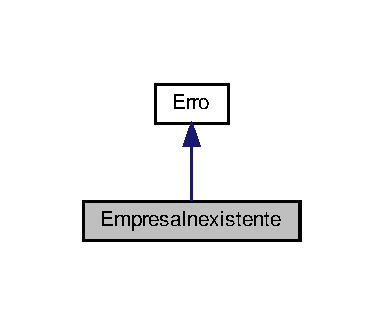
\includegraphics[width=184pt]{classEmpresaInexistente__inherit__graph}
\end{center}
\end{figure}


Collaboration diagram for Empresa\+Inexistente\+:
\nopagebreak
\begin{figure}[H]
\begin{center}
\leavevmode
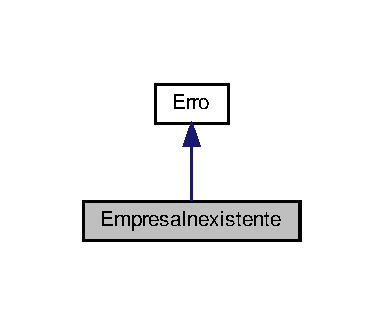
\includegraphics[width=184pt]{classEmpresaInexistente__coll__graph}
\end{center}
\end{figure}
\subsection*{Public Member Functions}
\begin{DoxyCompactItemize}
\item 
\hyperlink{classEmpresaInexistente_a96bfdab77510c1f330c6c66b7df19edd}{Empresa\+Inexistente} (const std\+::string \&info)
\begin{DoxyCompactList}\small\item\em Construtor da classe \hyperlink{classInputInvalido}{Input\+Invalido}. \end{DoxyCompactList}\end{DoxyCompactItemize}


\subsection{Constructor \& Destructor Documentation}
\mbox{\Hypertarget{classEmpresaInexistente_a96bfdab77510c1f330c6c66b7df19edd}\label{classEmpresaInexistente_a96bfdab77510c1f330c6c66b7df19edd}} 
\index{Empresa\+Inexistente@{Empresa\+Inexistente}!Empresa\+Inexistente@{Empresa\+Inexistente}}
\index{Empresa\+Inexistente@{Empresa\+Inexistente}!Empresa\+Inexistente@{Empresa\+Inexistente}}
\subsubsection{\texorpdfstring{Empresa\+Inexistente()}{EmpresaInexistente()}}
{\footnotesize\ttfamily Empresa\+Inexistente\+::\+Empresa\+Inexistente (\begin{DoxyParamCaption}\item[{const std\+::string \&}]{info }\end{DoxyParamCaption})\hspace{0.3cm}{\ttfamily [inline]}}



Construtor da classe \hyperlink{classInputInvalido}{Input\+Invalido}. 


\begin{DoxyCode}
181 : \hyperlink{classErro_a15d79796bd17517ff05d45eee55556f1}{Erro}(info) \{ \}
\end{DoxyCode}


The documentation for this class was generated from the following file\+:\begin{DoxyCompactItemize}
\item 
\hyperlink{Erro_8h}{Erro.\+h}\end{DoxyCompactItemize}

\hypertarget{classEmpresaJaAdicionada}{}\section{Empresa\+Ja\+Adicionada Class Reference}
\label{classEmpresaJaAdicionada}\index{Empresa\+Ja\+Adicionada@{Empresa\+Ja\+Adicionada}}


{\ttfamily \#include $<$Erro.\+h$>$}



Inheritance diagram for Empresa\+Ja\+Adicionada\+:
\nopagebreak
\begin{figure}[H]
\begin{center}
\leavevmode
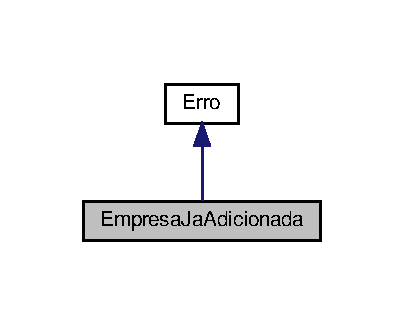
\includegraphics[width=194pt]{classEmpresaJaAdicionada__inherit__graph}
\end{center}
\end{figure}


Collaboration diagram for Empresa\+Ja\+Adicionada\+:
\nopagebreak
\begin{figure}[H]
\begin{center}
\leavevmode
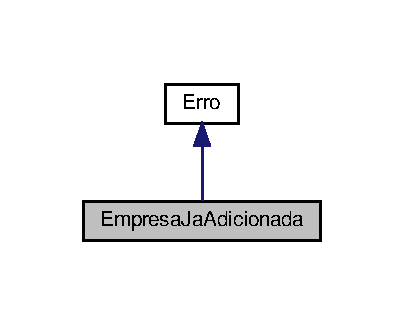
\includegraphics[width=194pt]{classEmpresaJaAdicionada__coll__graph}
\end{center}
\end{figure}
\subsection*{Public Member Functions}
\begin{DoxyCompactItemize}
\item 
\hyperlink{classEmpresaJaAdicionada_a31a58cd9fd890fc30edd073a560b1a6e}{Empresa\+Ja\+Adicionada} (const std\+::string \&info)
\begin{DoxyCompactList}\small\item\em Construtor da classe \hyperlink{classInputInvalido}{Input\+Invalido}. \end{DoxyCompactList}\end{DoxyCompactItemize}


\subsection{Constructor \& Destructor Documentation}
\mbox{\Hypertarget{classEmpresaJaAdicionada_a31a58cd9fd890fc30edd073a560b1a6e}\label{classEmpresaJaAdicionada_a31a58cd9fd890fc30edd073a560b1a6e}} 
\index{Empresa\+Ja\+Adicionada@{Empresa\+Ja\+Adicionada}!Empresa\+Ja\+Adicionada@{Empresa\+Ja\+Adicionada}}
\index{Empresa\+Ja\+Adicionada@{Empresa\+Ja\+Adicionada}!Empresa\+Ja\+Adicionada@{Empresa\+Ja\+Adicionada}}
\subsubsection{\texorpdfstring{Empresa\+Ja\+Adicionada()}{EmpresaJaAdicionada()}}
{\footnotesize\ttfamily Empresa\+Ja\+Adicionada\+::\+Empresa\+Ja\+Adicionada (\begin{DoxyParamCaption}\item[{const std\+::string \&}]{info }\end{DoxyParamCaption})\hspace{0.3cm}{\ttfamily [inline]}}



Construtor da classe \hyperlink{classInputInvalido}{Input\+Invalido}. 


\begin{DoxyCode}
189 : \hyperlink{classErro_a15d79796bd17517ff05d45eee55556f1}{Erro}(info) \{ \}
\end{DoxyCode}


The documentation for this class was generated from the following file\+:\begin{DoxyCompactItemize}
\item 
\hyperlink{Erro_8h}{Erro.\+h}\end{DoxyCompactItemize}

\hypertarget{structEmpresasComp}{}\section{Empresas\+Comp Struct Reference}
\label{structEmpresasComp}\index{Empresas\+Comp@{Empresas\+Comp}}


{\ttfamily \#include $<$Empresa.\+h$>$}

\subsection*{Public Member Functions}
\begin{DoxyCompactItemize}
\item 
bool \hyperlink{structEmpresasComp_a65f437399b6aa939ee84611a69ee0ad0}{operator()} (\hyperlink{classEmpresa}{Empresa} $\ast$empresa1, \hyperlink{classEmpresa}{Empresa} $\ast$empresa2) const
\end{DoxyCompactItemize}


\subsection{Member Function Documentation}
\mbox{\Hypertarget{structEmpresasComp_a65f437399b6aa939ee84611a69ee0ad0}\label{structEmpresasComp_a65f437399b6aa939ee84611a69ee0ad0}} 
\index{Empresas\+Comp@{Empresas\+Comp}!operator()@{operator()}}
\index{operator()@{operator()}!Empresas\+Comp@{Empresas\+Comp}}
\subsubsection{\texorpdfstring{operator()()}{operator()()}}
{\footnotesize\ttfamily bool Empresas\+Comp\+::operator() (\begin{DoxyParamCaption}\item[{\hyperlink{classEmpresa}{Empresa} $\ast$}]{empresa1,  }\item[{\hyperlink{classEmpresa}{Empresa} $\ast$}]{empresa2 }\end{DoxyParamCaption}) const\hspace{0.3cm}{\ttfamily [inline]}}


\begin{DoxyCode}
95     \{
96         \textcolor{keywordflow}{if} (empresa1->\hyperlink{classEmpresa_a49b2b94a54bbc341822f64fc194f98fd}{getNumeroTitulos}() == empresa2->
      \hyperlink{classEmpresa_a49b2b94a54bbc341822f64fc194f98fd}{getNumeroTitulos}())
97             \textcolor{keywordflow}{return} empresa1->\hyperlink{classEmpresa_a99bc2de98a0c0348abb74c93e6e7159e}{getNomeEmpresa}() < empresa2->
      \hyperlink{classEmpresa_a99bc2de98a0c0348abb74c93e6e7159e}{getNomeEmpresa}();
98         \textcolor{keywordflow}{return} empresa1->\hyperlink{classEmpresa_a49b2b94a54bbc341822f64fc194f98fd}{getNumeroTitulos}() < empresa2->
      \hyperlink{classEmpresa_a49b2b94a54bbc341822f64fc194f98fd}{getNumeroTitulos}();
99     \}
\end{DoxyCode}
Here is the call graph for this function\+:
\nopagebreak
\begin{figure}[H]
\begin{center}
\leavevmode
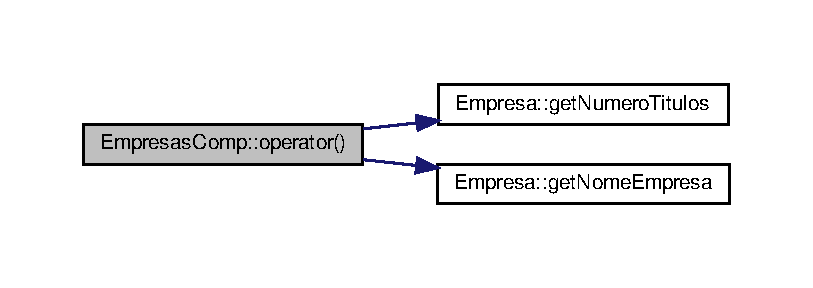
\includegraphics[width=350pt]{structEmpresasComp_a65f437399b6aa939ee84611a69ee0ad0_cgraph}
\end{center}
\end{figure}


The documentation for this struct was generated from the following file\+:\begin{DoxyCompactItemize}
\item 
\hyperlink{Empresa_8h}{Empresa.\+h}\end{DoxyCompactItemize}

\hypertarget{classErro}{}\section{Erro Class Reference}
\label{classErro}\index{Erro@{Erro}}


{\ttfamily \#include $<$Erro.\+h$>$}



Inheritance diagram for Erro\+:
\nopagebreak
\begin{figure}[H]
\begin{center}
\leavevmode
\includegraphics[height=550pt]{classErro__inherit__graph}
\end{center}
\end{figure}
\subsection*{Public Member Functions}
\begin{DoxyCompactItemize}
\item 
\hyperlink{classErro_a15d79796bd17517ff05d45eee55556f1}{Erro} (const std\+::string \&info)
\begin{DoxyCompactList}\small\item\em Construtor da classe \hyperlink{classErro}{Erro}. \end{DoxyCompactList}\item 
const std\+::string \hyperlink{classErro_abfc1e9735b259d88bb97828a23164eb0}{get\+Info} () const
\begin{DoxyCompactList}\small\item\em Permite obter a descricao do \hyperlink{classErro}{Erro}. \end{DoxyCompactList}\end{DoxyCompactItemize}


\subsection{Detailed Description}
Classe \hyperlink{classErro}{Erro} utilizada para tratamento de excecoes no decorrer do programa. 

\subsection{Constructor \& Destructor Documentation}
\mbox{\Hypertarget{classErro_a15d79796bd17517ff05d45eee55556f1}\label{classErro_a15d79796bd17517ff05d45eee55556f1}} 
\index{Erro@{Erro}!Erro@{Erro}}
\index{Erro@{Erro}!Erro@{Erro}}
\subsubsection{\texorpdfstring{Erro()}{Erro()}}
{\footnotesize\ttfamily Erro\+::\+Erro (\begin{DoxyParamCaption}\item[{const std\+::string \&}]{info }\end{DoxyParamCaption})\hspace{0.3cm}{\ttfamily [inline]}}



Construtor da classe \hyperlink{classErro}{Erro}. 


\begin{DoxyParams}{Parameters}
{\em info} & -\/ Descricao do tipo de erro que aconteceu aquando o lancamento de uma excecao \\
\hline
\end{DoxyParams}

\begin{DoxyCode}
17 : info(info) \{\}
\end{DoxyCode}


\subsection{Member Function Documentation}
\mbox{\Hypertarget{classErro_abfc1e9735b259d88bb97828a23164eb0}\label{classErro_abfc1e9735b259d88bb97828a23164eb0}} 
\index{Erro@{Erro}!get\+Info@{get\+Info}}
\index{get\+Info@{get\+Info}!Erro@{Erro}}
\subsubsection{\texorpdfstring{get\+Info()}{getInfo()}}
{\footnotesize\ttfamily const std\+::string Erro\+::get\+Info (\begin{DoxyParamCaption}{ }\end{DoxyParamCaption}) const\hspace{0.3cm}{\ttfamily [inline]}}



Permite obter a descricao do \hyperlink{classErro}{Erro}. 

\begin{DoxyReturn}{Returns}
Retorna a descricao do \hyperlink{classErro}{Erro} 
\end{DoxyReturn}

\begin{DoxyCode}
23 \{ \textcolor{keywordflow}{return} info; \}
\end{DoxyCode}
Here is the caller graph for this function\+:
\nopagebreak
\begin{figure}[H]
\begin{center}
\leavevmode
\includegraphics[width=350pt]{classErro_abfc1e9735b259d88bb97828a23164eb0_icgraph}
\end{center}
\end{figure}


The documentation for this class was generated from the following file\+:\begin{DoxyCompactItemize}
\item 
\hyperlink{Erro_8h}{Erro.\+h}\end{DoxyCompactItemize}

\hypertarget{classErroEmail}{}\section{Erro\+Email Class Reference}
\label{classErroEmail}\index{Erro\+Email@{Erro\+Email}}


{\ttfamily \#include $<$Erro.\+h$>$}



Inheritance diagram for Erro\+Email\+:
\nopagebreak
\begin{figure}[H]
\begin{center}
\leavevmode
\includegraphics[width=139pt]{classErroEmail__inherit__graph}
\end{center}
\end{figure}


Collaboration diagram for Erro\+Email\+:
\nopagebreak
\begin{figure}[H]
\begin{center}
\leavevmode
\includegraphics[width=139pt]{classErroEmail__coll__graph}
\end{center}
\end{figure}
\subsection*{Public Member Functions}
\begin{DoxyCompactItemize}
\item 
\hyperlink{classErroEmail_a536520637b17434e8fd8ab296db9e026}{Erro\+Email} (const std\+::string \&info)
\begin{DoxyCompactList}\small\item\em Construtor da classe \hyperlink{classUtilizadorInexistente}{Utilizador\+Inexistente}. \end{DoxyCompactList}\end{DoxyCompactItemize}


\subsection{Constructor \& Destructor Documentation}
\mbox{\Hypertarget{classErroEmail_a536520637b17434e8fd8ab296db9e026}\label{classErroEmail_a536520637b17434e8fd8ab296db9e026}} 
\index{Erro\+Email@{Erro\+Email}!Erro\+Email@{Erro\+Email}}
\index{Erro\+Email@{Erro\+Email}!Erro\+Email@{Erro\+Email}}
\subsubsection{\texorpdfstring{Erro\+Email()}{ErroEmail()}}
{\footnotesize\ttfamily Erro\+Email\+::\+Erro\+Email (\begin{DoxyParamCaption}\item[{const std\+::string \&}]{info }\end{DoxyParamCaption})\hspace{0.3cm}{\ttfamily [inline]}}



Construtor da classe \hyperlink{classUtilizadorInexistente}{Utilizador\+Inexistente}. 


\begin{DoxyCode}
170 : \hyperlink{classErro_a15d79796bd17517ff05d45eee55556f1}{Erro}(info) \{ \}
\end{DoxyCode}


The documentation for this class was generated from the following file\+:\begin{DoxyCompactItemize}
\item 
\hyperlink{Erro_8h}{Erro.\+h}\end{DoxyCompactItemize}

\hypertarget{classHome}{}\section{Home Class Reference}
\label{classHome}\index{Home@{Home}}


{\ttfamily \#include $<$Titulo.\+h$>$}



Inheritance diagram for Home\+:
\nopagebreak
\begin{figure}[H]
\begin{center}
\leavevmode
\includegraphics[width=123pt]{classHome__inherit__graph}
\end{center}
\end{figure}


Collaboration diagram for Home\+:
\nopagebreak
\begin{figure}[H]
\begin{center}
\leavevmode
\includegraphics[width=178pt]{classHome__coll__graph}
\end{center}
\end{figure}
\subsection*{Public Member Functions}
\begin{DoxyCompactItemize}
\item 
\hyperlink{classHome_aea37c4a72119815e8e0a83b63f345cc9}{Home} (std\+::string \hyperlink{classTitulo_a8abdf1fc6d4fc14be20bbec247664d83}{nome}, int \hyperlink{classTitulo_a28891078f53fc3317de60ae739514955}{idade\+Minima}, std\+::string \hyperlink{classTitulo_a67761eb7f006453ab0869e4b7c0a9c0b}{plataforma}, float preco, std\+::vector$<$ std\+::string $>$ \hyperlink{classTitulo_a3209265c8534416978ee9891b96c14b2}{generos}, std\+::string \hyperlink{classTitulo_a91510c440dc8583d60d88ea02f4eb1b6}{empresa}, \hyperlink{classData}{Data} \hyperlink{classTitulo_ae540ddf2c607eb0e4de29eb8c0cca7f0}{data\+Lancamento}, unsigned int numero, unsigned int cliques)
\begin{DoxyCompactList}\small\item\em construtor da classe \hyperlink{classHome}{Home} \end{DoxyCompactList}\item 
bool \hyperlink{classHome_a94aec68b520d98ac38c6794b5771cd53}{adiciona\+Atualizacao} (const \hyperlink{classData}{Data} \&D)
\begin{DoxyCompactList}\small\item\em Adiciona uma data ao vetor data\+\_\+de\+\_\+atualizacao. \end{DoxyCompactList}\item 
unsigned int \hyperlink{classHome_a52f37198fb17a321dbcac93d1c35b537}{get\+Preco\+Atualizacao} () const
\begin{DoxyCompactList}\small\item\em Devolve o preco por atualizacao. \end{DoxyCompactList}\item 
std\+::vector$<$ \hyperlink{classData}{Data} $>$ \hyperlink{classHome_a0ab7279a76525f48cb1b64b8bae98a44}{get\+Datas} () const
\begin{DoxyCompactList}\small\item\em Devolve membro dado vetor de datas. \end{DoxyCompactList}\item 
float \hyperlink{classHome_aff6d69739d404378524a591596b47856}{get\+Gastos} () const
\begin{DoxyCompactList}\small\item\em Devolve os gastos associados as atualizacoes. \end{DoxyCompactList}\end{DoxyCompactItemize}
\subsection*{Additional Inherited Members}


\subsection{Detailed Description}
\hyperlink{classHome}{Home} derivada de \hyperlink{classTitulo}{Titulo} 

\subsection{Constructor \& Destructor Documentation}
\mbox{\Hypertarget{classHome_aea37c4a72119815e8e0a83b63f345cc9}\label{classHome_aea37c4a72119815e8e0a83b63f345cc9}} 
\index{Home@{Home}!Home@{Home}}
\index{Home@{Home}!Home@{Home}}
\subsubsection{\texorpdfstring{Home()}{Home()}}
{\footnotesize\ttfamily Home\+::\+Home (\begin{DoxyParamCaption}\item[{std\+::string}]{nome,  }\item[{int}]{idade\+Minima,  }\item[{std\+::string}]{plataforma,  }\item[{float}]{preco,  }\item[{std\+::vector$<$ std\+::string $>$}]{generos,  }\item[{std\+::string}]{empresa,  }\item[{\hyperlink{classData}{Data}}]{data\+Lancamento,  }\item[{unsigned int}]{numero,  }\item[{unsigned int}]{cliques }\end{DoxyParamCaption})}



construtor da classe \hyperlink{classHome}{Home} 


\begin{DoxyParams}{Parameters}
{\em nome} & -\/ Nome atribuido ao titulo \\
\hline
{\em idade\+Minima} & -\/ Idade minima atribuida ao titulo \\
\hline
{\em plataforma} & -\/ Plataforma atribuida ao titulo \\
\hline
{\em preco} & -\/ Preco base adicionado ao historico de precos \\
\hline
{\em generos} & -\/ Generos atribuidos ao titulo \\
\hline
{\em empresa} & -\/ \hyperlink{classEmpresa}{Empresa} atribuida ao titulo \\
\hline
{\em data\+Lancamento} & -\/ \hyperlink{classData}{Data} atribuida ao titulo \\
\hline
{\em numero} & -\/ Numero de anuncios visualizados \\
\hline
{\em cliques} & -\/ Numero de cliques no titulo \\
\hline
\end{DoxyParams}

\begin{DoxyCode}
180                                                                             :
181         \hyperlink{classTitulo_a898faeefdad15c64ae4cdc904a7e6f0e}{Titulo}(\hyperlink{classTitulo_a8abdf1fc6d4fc14be20bbec247664d83}{nome}, \hyperlink{classTitulo_a28891078f53fc3317de60ae739514955}{idadeMinima}, \hyperlink{classTitulo_a67761eb7f006453ab0869e4b7c0a9c0b}{plataforma},preco, 
      \hyperlink{classTitulo_a3209265c8534416978ee9891b96c14b2}{generos}, \hyperlink{classTitulo_a91510c440dc8583d60d88ea02f4eb1b6}{empresa},
182                 dataLancamento, numero, cliques) \{
183 
184  \}
\end{DoxyCode}


\subsection{Member Function Documentation}
\mbox{\Hypertarget{classHome_a94aec68b520d98ac38c6794b5771cd53}\label{classHome_a94aec68b520d98ac38c6794b5771cd53}} 
\index{Home@{Home}!adiciona\+Atualizacao@{adiciona\+Atualizacao}}
\index{adiciona\+Atualizacao@{adiciona\+Atualizacao}!Home@{Home}}
\subsubsection{\texorpdfstring{adiciona\+Atualizacao()}{adicionaAtualizacao()}}
{\footnotesize\ttfamily bool Home\+::adiciona\+Atualizacao (\begin{DoxyParamCaption}\item[{const \hyperlink{classData}{Data} \&}]{D }\end{DoxyParamCaption})}



Adiciona uma data ao vetor data\+\_\+de\+\_\+atualizacao. 


\begin{DoxyParams}{Parameters}
{\em D} & -\/ data em que houve uma atualizacao \\
\hline
\end{DoxyParams}
\begin{DoxyReturn}{Returns}
Retorna verdade ou falso se for possivel adicionar ao vetor a data 
\end{DoxyReturn}

\begin{DoxyCode}
188                                               \{
189 
190     \textcolor{keywordflow}{if} (find(this->dataDeAtualizacao.begin(), this->dataDeAtualizacao.end(),
191             D) != this->dataDeAtualizacao.end())
192         \textcolor{keywordflow}{return} \textcolor{keyword}{false};
193     \textcolor{keywordflow}{else} \{
194         this->dataDeAtualizacao.push\_back(D);
195         \textcolor{keywordflow}{return} \textcolor{keyword}{true};
196     \}
197 
198  \}
\end{DoxyCode}
Here is the caller graph for this function\+:
\nopagebreak
\begin{figure}[H]
\begin{center}
\leavevmode
\includegraphics[width=350pt]{classHome_a94aec68b520d98ac38c6794b5771cd53_icgraph}
\end{center}
\end{figure}
\mbox{\Hypertarget{classHome_a0ab7279a76525f48cb1b64b8bae98a44}\label{classHome_a0ab7279a76525f48cb1b64b8bae98a44}} 
\index{Home@{Home}!get\+Datas@{get\+Datas}}
\index{get\+Datas@{get\+Datas}!Home@{Home}}
\subsubsection{\texorpdfstring{get\+Datas()}{getDatas()}}
{\footnotesize\ttfamily std\+::vector$<$ \hyperlink{classData}{Data} $>$ Home\+::get\+Datas (\begin{DoxyParamCaption}{ }\end{DoxyParamCaption}) const}



Devolve membro dado vetor de datas. 

\begin{DoxyReturn}{Returns}
Retorna vetor de datas de atualizacao 
\end{DoxyReturn}

\begin{DoxyCode}
210  \{
211     \textcolor{keywordflow}{return} this->dataDeAtualizacao;
212  \}
\end{DoxyCode}
Here is the caller graph for this function\+:
\nopagebreak
\begin{figure}[H]
\begin{center}
\leavevmode
\includegraphics[width=350pt]{classHome_a0ab7279a76525f48cb1b64b8bae98a44_icgraph}
\end{center}
\end{figure}
\mbox{\Hypertarget{classHome_aff6d69739d404378524a591596b47856}\label{classHome_aff6d69739d404378524a591596b47856}} 
\index{Home@{Home}!get\+Gastos@{get\+Gastos}}
\index{get\+Gastos@{get\+Gastos}!Home@{Home}}
\subsubsection{\texorpdfstring{get\+Gastos()}{getGastos()}}
{\footnotesize\ttfamily float Home\+::get\+Gastos (\begin{DoxyParamCaption}{ }\end{DoxyParamCaption}) const\hspace{0.3cm}{\ttfamily [virtual]}}



Devolve os gastos associados as atualizacoes. 

\begin{DoxyReturn}{Returns}
Retorna os gastos 
\end{DoxyReturn}


Implements \hyperlink{classTitulo_a9272448eec05cd9c026c54824bf2e727}{Titulo}.


\begin{DoxyCode}
234  \{
235     \textcolor{keywordtype}{float} total = dataDeAtualizacao.size()* this->precoAtualizacao;
236     \textcolor{keywordflow}{return} total;
237  \}
\end{DoxyCode}
\mbox{\Hypertarget{classHome_a52f37198fb17a321dbcac93d1c35b537}\label{classHome_a52f37198fb17a321dbcac93d1c35b537}} 
\index{Home@{Home}!get\+Preco\+Atualizacao@{get\+Preco\+Atualizacao}}
\index{get\+Preco\+Atualizacao@{get\+Preco\+Atualizacao}!Home@{Home}}
\subsubsection{\texorpdfstring{get\+Preco\+Atualizacao()}{getPrecoAtualizacao()}}
{\footnotesize\ttfamily unsigned int Home\+::get\+Preco\+Atualizacao (\begin{DoxyParamCaption}{ }\end{DoxyParamCaption}) const}



Devolve o preco por atualizacao. 

\begin{DoxyReturn}{Returns}
Retorna o membro dato precoatualizacao 
\end{DoxyReturn}

\begin{DoxyCode}
203  \{
204     \textcolor{keywordflow}{return} this->precoAtualizacao;
205  \}
\end{DoxyCode}
Here is the caller graph for this function\+:
\nopagebreak
\begin{figure}[H]
\begin{center}
\leavevmode
\includegraphics[width=319pt]{classHome_a52f37198fb17a321dbcac93d1c35b537_icgraph}
\end{center}
\end{figure}


The documentation for this class was generated from the following files\+:\begin{DoxyCompactItemize}
\item 
\hyperlink{Titulo_8h}{Titulo.\+h}\item 
\hyperlink{Titulo_8cpp}{Titulo.\+cpp}\end{DoxyCompactItemize}

\hypertarget{classInputInvalido}{}\section{Input\+Invalido Class Reference}
\label{classInputInvalido}\index{Input\+Invalido@{Input\+Invalido}}


{\ttfamily \#include $<$Erro.\+h$>$}



Inheritance diagram for Input\+Invalido\+:
\nopagebreak
\begin{figure}[H]
\begin{center}
\leavevmode
\includegraphics[width=152pt]{classInputInvalido__inherit__graph}
\end{center}
\end{figure}


Collaboration diagram for Input\+Invalido\+:
\nopagebreak
\begin{figure}[H]
\begin{center}
\leavevmode
\includegraphics[width=152pt]{classInputInvalido__coll__graph}
\end{center}
\end{figure}
\subsection*{Public Member Functions}
\begin{DoxyCompactItemize}
\item 
\hyperlink{classInputInvalido_aa24dddc4e0de404949099c741266e193}{Input\+Invalido} (const std\+::string \&info)
\begin{DoxyCompactList}\small\item\em Construtor da classe \hyperlink{classInputInvalido}{Input\+Invalido}. \end{DoxyCompactList}\end{DoxyCompactItemize}


\subsection{Constructor \& Destructor Documentation}
\mbox{\Hypertarget{classInputInvalido_aa24dddc4e0de404949099c741266e193}\label{classInputInvalido_aa24dddc4e0de404949099c741266e193}} 
\index{Input\+Invalido@{Input\+Invalido}!Input\+Invalido@{Input\+Invalido}}
\index{Input\+Invalido@{Input\+Invalido}!Input\+Invalido@{Input\+Invalido}}
\subsubsection{\texorpdfstring{Input\+Invalido()}{InputInvalido()}}
{\footnotesize\ttfamily Input\+Invalido\+::\+Input\+Invalido (\begin{DoxyParamCaption}\item[{const std\+::string \&}]{info }\end{DoxyParamCaption})\hspace{0.3cm}{\ttfamily [inline]}}



Construtor da classe \hyperlink{classInputInvalido}{Input\+Invalido}. 


\begin{DoxyCode}
148 : \hyperlink{classErro_a15d79796bd17517ff05d45eee55556f1}{Erro}(info) \{ \}
\end{DoxyCode}


The documentation for this class was generated from the following file\+:\begin{DoxyCompactItemize}
\item 
\hyperlink{Erro_8h}{Erro.\+h}\end{DoxyCompactItemize}

\hypertarget{classOnline}{}\section{Online Class Reference}
\label{classOnline}\index{Online@{Online}}


{\ttfamily \#include $<$Titulo.\+h$>$}



Inheritance diagram for Online\+:
\nopagebreak
\begin{figure}[H]
\begin{center}
\leavevmode
\includegraphics[width=124pt]{classOnline__inherit__graph}
\end{center}
\end{figure}


Collaboration diagram for Online\+:
\nopagebreak
\begin{figure}[H]
\begin{center}
\leavevmode
\includegraphics[width=178pt]{classOnline__coll__graph}
\end{center}
\end{figure}
\subsection*{Public Member Functions}
\begin{DoxyCompactItemize}
\item 
\hyperlink{classOnline_ae6a934ef34ed86ab205190f2b632366a}{Online} (std\+::string \hyperlink{classTitulo_a8abdf1fc6d4fc14be20bbec247664d83}{nome}, int \hyperlink{classTitulo_a28891078f53fc3317de60ae739514955}{idade\+Minima}, std\+::string \hyperlink{classTitulo_a67761eb7f006453ab0869e4b7c0a9c0b}{plataforma}, float preco, std\+::vector$<$ std\+::string $>$ \hyperlink{classTitulo_a3209265c8534416978ee9891b96c14b2}{generos}, std\+::string \hyperlink{classTitulo_a91510c440dc8583d60d88ea02f4eb1b6}{empresa}, \hyperlink{classData}{Data} \hyperlink{classTitulo_ae540ddf2c607eb0e4de29eb8c0cca7f0}{data\+Lancamento}, unsigned int numero, unsigned int cliques, bool subs, float p\+Subscricao)
\begin{DoxyCompactList}\small\item\em construtor da classe \hyperlink{classOnline}{Online} \end{DoxyCompactList}\item 
std\+::vector$<$ \hyperlink{classData}{Data} $>$ \hyperlink{classOnline_aa6f51a948cb5ffd2c7cbac1f1cd6023f}{get\+Datas\+Jogo} () const
\begin{DoxyCompactList}\small\item\em Devolve as datas jogadas. \end{DoxyCompactList}\item 
std\+::vector$<$ unsigned int $>$ \hyperlink{classOnline_a4ab18dfdaa0af23cda8f5268a9968887}{get\+Minutos\+Jogo} () const
\begin{DoxyCompactList}\small\item\em Devolve os minutos jogados por data. \end{DoxyCompactList}\item 
void \hyperlink{classOnline_a71cc818cd9b8020a470efc14f636a9f9}{set\+Minutos\+Jogo} (std\+::vector$<$ unsigned int $>$ \&minutosjogo)
\begin{DoxyCompactList}\small\item\em Altera os minutos jogados por data. \end{DoxyCompactList}\item 
void \hyperlink{classOnline_a3c0b8d3393271eabfa702629c979fb93}{set\+Datas\+Jogo} (std\+::vector$<$ \hyperlink{classData}{Data} $>$ \&datas\+Jogo)
\begin{DoxyCompactList}\small\item\em Altera as datas jogadas. \end{DoxyCompactList}\item 
void \hyperlink{classOnline_a1796bfbb1c3210f26ca8e1cddc61d830}{atualiza\+Est\+Aux} (const \hyperlink{classData}{Data} \&D1, const size\+\_\+t minutos)
\begin{DoxyCompactList}\small\item\em Adiciona aos 3 vetores os habitos gaming de uma certa data, funcao a usar em adiciona\+Estatisticas. \end{DoxyCompactList}\item 
void \hyperlink{classOnline_aac2ef3483edfaa8426363ebdd542dc38}{adiciona\+Estatisticas} (const \hyperlink{classData}{Data} \&D1, const size\+\_\+t minutos)
\begin{DoxyCompactList}\small\item\em Adicionar estaticas relativas aos habitos de gaming, atualiza os 3 ultimos vetores, cuja ordem � crucial e atualiza horas\+\_\+totais. \end{DoxyCompactList}\item 
float \hyperlink{classOnline_ad0a23d2f1a2f804479ff346be0fdc686}{get\+Horas\+Totais} () const
\begin{DoxyCompactList}\small\item\em Devolve o numero de horas jogadas, arredondando para cima o membro estatico horas totais. \end{DoxyCompactList}\item 
bool \hyperlink{classOnline_aa222489df5a1e6bcfbf5e01d95178850}{get\+Subscricao} () const
\begin{DoxyCompactList}\small\item\em Devolve o booleano que indica se o jogo tem uma subscricao fixa ou variavel. \end{DoxyCompactList}\item 
float \hyperlink{classOnline_a0f7240aa5582e10579d0719e4fa5d705}{get\+Preco\+Subscricao} () const
\begin{DoxyCompactList}\small\item\em Devolve o preco por subscricao. \end{DoxyCompactList}\item 
float \hyperlink{classOnline_ac3a2197523ee26effcacd9a2a9fe968e}{get\+Gastos} () const
\begin{DoxyCompactList}\small\item\em Devolve os gastos associadas a subscricao. \end{DoxyCompactList}\end{DoxyCompactItemize}
\subsection*{Additional Inherited Members}


\subsection{Detailed Description}
\hyperlink{classOnline}{Online} derivada de \hyperlink{classTitulo}{Titulo} 

\subsection{Constructor \& Destructor Documentation}
\mbox{\Hypertarget{classOnline_ae6a934ef34ed86ab205190f2b632366a}\label{classOnline_ae6a934ef34ed86ab205190f2b632366a}} 
\index{Online@{Online}!Online@{Online}}
\index{Online@{Online}!Online@{Online}}
\subsubsection{\texorpdfstring{Online()}{Online()}}
{\footnotesize\ttfamily Online\+::\+Online (\begin{DoxyParamCaption}\item[{std\+::string}]{nome,  }\item[{int}]{idade\+Minima,  }\item[{std\+::string}]{plataforma,  }\item[{float}]{preco,  }\item[{std\+::vector$<$ std\+::string $>$}]{generos,  }\item[{std\+::string}]{empresa,  }\item[{\hyperlink{classData}{Data}}]{data\+Lancamento,  }\item[{unsigned int}]{numero,  }\item[{unsigned int}]{cliques,  }\item[{bool}]{subs,  }\item[{float}]{p\+Subscricao }\end{DoxyParamCaption})}



construtor da classe \hyperlink{classOnline}{Online} 


\begin{DoxyParams}{Parameters}
{\em nome} & -\/ Nome atribuido ao titulo \\
\hline
{\em idade\+Minima} & -\/ Idade minima atribuida ao titulo \\
\hline
{\em plataforma} & -\/ Plataforma atribuida ao titulo \\
\hline
{\em preco} & -\/ Preco base adicionado ao historico de precos \\
\hline
{\em generos} & -\/ Generos atribuidos ao titulo \\
\hline
{\em empresa} & -\/ \hyperlink{classEmpresa}{Empresa} atribuida ao titulo \\
\hline
{\em data\+Lancamento} & -\/ \hyperlink{classData}{Data} atribuida ao titulo \\
\hline
{\em subs} & -\/ Subscricao fixa ou variavel \\
\hline
{\em -\/} & Preco da subscricao escolhida \\
\hline
{\em numero} & -\/ Numero de anuncios visualizados \\
\hline
{\em cliques} & -\/ Numero de cliques no titulo \\
\hline
\end{DoxyParams}

\begin{DoxyCode}
244                                                                                                           :
245         \hyperlink{classTitulo_a898faeefdad15c64ae4cdc904a7e6f0e}{Titulo}(\hyperlink{classTitulo_a8abdf1fc6d4fc14be20bbec247664d83}{nome}, \hyperlink{classTitulo_a28891078f53fc3317de60ae739514955}{idadeMinima}, \hyperlink{classTitulo_a67761eb7f006453ab0869e4b7c0a9c0b}{plataforma},preco, 
      \hyperlink{classTitulo_a3209265c8534416978ee9891b96c14b2}{generos}, \hyperlink{classTitulo_a91510c440dc8583d60d88ea02f4eb1b6}{empresa},
246                 dataLancamento, numero, cliques) \{
247     this->subscricaoFixa = subs;
248     this->precoSubscricao = pSubscricao;
249     horasTotais=0;
250  \}
\end{DoxyCode}


\subsection{Member Function Documentation}
\mbox{\Hypertarget{classOnline_aac2ef3483edfaa8426363ebdd542dc38}\label{classOnline_aac2ef3483edfaa8426363ebdd542dc38}} 
\index{Online@{Online}!adiciona\+Estatisticas@{adiciona\+Estatisticas}}
\index{adiciona\+Estatisticas@{adiciona\+Estatisticas}!Online@{Online}}
\subsubsection{\texorpdfstring{adiciona\+Estatisticas()}{adicionaEstatisticas()}}
{\footnotesize\ttfamily void Online\+::adiciona\+Estatisticas (\begin{DoxyParamCaption}\item[{const \hyperlink{classData}{Data} \&}]{D1,  }\item[{const size\+\_\+t}]{minutos }\end{DoxyParamCaption})}



Adicionar estaticas relativas aos habitos de gaming, atualiza os 3 ultimos vetores, cuja ordem � crucial e atualiza horas\+\_\+totais. 


\begin{DoxyParams}{Parameters}
{\em D1} & -\/ data em que jogou, podendo jogar mais que uma vez ao dia,na mesma plataforma ou nao \\
\hline
{\em minutos} & -\/ tempo que jogou \\
\hline
\end{DoxyParams}

\begin{DoxyCode}
277                                                                         \{
278 
279     \textcolor{keywordtype}{unsigned} \textcolor{keywordtype}{int} indiceData = 0;
280 
281     \textcolor{keywordflow}{for} (\textcolor{keyword}{auto} data : this->datasEmQueJogou) \{
282         \textcolor{keywordflow}{if} (data == D1) \{
283             this->minutosJogadosPorData[indiceData] += minutos; \textcolor{comment}{/*atualiza os minutos numa data*/}
284             horasTotais += minutos / 60.0;
285             \textcolor{keywordflow}{return};
286         \}
287 
288         indiceData++;
289     \}
290 
291     \hyperlink{classOnline_a1796bfbb1c3210f26ca8e1cddc61d830}{atualizaEstAux}(D1, minutos);
292     horasTotais += minutos / 60.0;
293 
294     \textcolor{keywordflow}{return};
295  \}
\end{DoxyCode}
Here is the call graph for this function\+:
\nopagebreak
\begin{figure}[H]
\begin{center}
\leavevmode
\includegraphics[width=350pt]{classOnline_aac2ef3483edfaa8426363ebdd542dc38_cgraph}
\end{center}
\end{figure}
Here is the caller graph for this function\+:
\nopagebreak
\begin{figure}[H]
\begin{center}
\leavevmode
\includegraphics[width=350pt]{classOnline_aac2ef3483edfaa8426363ebdd542dc38_icgraph}
\end{center}
\end{figure}
\mbox{\Hypertarget{classOnline_a1796bfbb1c3210f26ca8e1cddc61d830}\label{classOnline_a1796bfbb1c3210f26ca8e1cddc61d830}} 
\index{Online@{Online}!atualiza\+Est\+Aux@{atualiza\+Est\+Aux}}
\index{atualiza\+Est\+Aux@{atualiza\+Est\+Aux}!Online@{Online}}
\subsubsection{\texorpdfstring{atualiza\+Est\+Aux()}{atualizaEstAux()}}
{\footnotesize\ttfamily void Online\+::atualiza\+Est\+Aux (\begin{DoxyParamCaption}\item[{const \hyperlink{classData}{Data} \&}]{D1,  }\item[{const size\+\_\+t}]{minutos }\end{DoxyParamCaption})}



Adiciona aos 3 vetores os habitos gaming de uma certa data, funcao a usar em adiciona\+Estatisticas. 


\begin{DoxyParams}{Parameters}
{\em D1} & -\/ data em que jogou \\
\hline
{\em minutos} & -\/ tempo que jogou \\
\hline
\end{DoxyParams}

\begin{DoxyCode}
270                                                                   \{
271     this->datasEmQueJogou.push\_back(D1);
272     this->minutosJogadosPorData.push\_back(minutos);
273  \}
\end{DoxyCode}
Here is the caller graph for this function\+:
\nopagebreak
\begin{figure}[H]
\begin{center}
\leavevmode
\includegraphics[width=350pt]{classOnline_a1796bfbb1c3210f26ca8e1cddc61d830_icgraph}
\end{center}
\end{figure}
\mbox{\Hypertarget{classOnline_aa6f51a948cb5ffd2c7cbac1f1cd6023f}\label{classOnline_aa6f51a948cb5ffd2c7cbac1f1cd6023f}} 
\index{Online@{Online}!get\+Datas\+Jogo@{get\+Datas\+Jogo}}
\index{get\+Datas\+Jogo@{get\+Datas\+Jogo}!Online@{Online}}
\subsubsection{\texorpdfstring{get\+Datas\+Jogo()}{getDatasJogo()}}
{\footnotesize\ttfamily std\+::vector$<$ \hyperlink{classData}{Data} $>$ Online\+::get\+Datas\+Jogo (\begin{DoxyParamCaption}{ }\end{DoxyParamCaption}) const}



Devolve as datas jogadas. 

\begin{DoxyReturn}{Returns}
Vetor com datas jogadas 
\end{DoxyReturn}

\begin{DoxyCode}
252                                           \{
253     \textcolor{keywordflow}{return} datasEmQueJogou;
254 \}
\end{DoxyCode}
Here is the caller graph for this function\+:
\nopagebreak
\begin{figure}[H]
\begin{center}
\leavevmode
\includegraphics[width=350pt]{classOnline_aa6f51a948cb5ffd2c7cbac1f1cd6023f_icgraph}
\end{center}
\end{figure}
\mbox{\Hypertarget{classOnline_ac3a2197523ee26effcacd9a2a9fe968e}\label{classOnline_ac3a2197523ee26effcacd9a2a9fe968e}} 
\index{Online@{Online}!get\+Gastos@{get\+Gastos}}
\index{get\+Gastos@{get\+Gastos}!Online@{Online}}
\subsubsection{\texorpdfstring{get\+Gastos()}{getGastos()}}
{\footnotesize\ttfamily float Online\+::get\+Gastos (\begin{DoxyParamCaption}{ }\end{DoxyParamCaption}) const\hspace{0.3cm}{\ttfamily [virtual]}}



Devolve os gastos associadas a subscricao. 

\begin{DoxyReturn}{Returns}
Retorna os gastos 
\end{DoxyReturn}


Implements \hyperlink{classTitulo_a9272448eec05cd9c026c54824bf2e727}{Titulo}.


\begin{DoxyCode}
324  \{
325      \textcolor{keywordtype}{float} total=0;
326      \textcolor{keywordflow}{if}(subscricaoFixa)
327          total+=precoSubscricao;
328      \textcolor{keywordflow}{else} total += (precoSubscricao*horasTotais);
329 
330      \textcolor{keywordflow}{return} total;
331  \}
\end{DoxyCode}
\mbox{\Hypertarget{classOnline_ad0a23d2f1a2f804479ff346be0fdc686}\label{classOnline_ad0a23d2f1a2f804479ff346be0fdc686}} 
\index{Online@{Online}!get\+Horas\+Totais@{get\+Horas\+Totais}}
\index{get\+Horas\+Totais@{get\+Horas\+Totais}!Online@{Online}}
\subsubsection{\texorpdfstring{get\+Horas\+Totais()}{getHorasTotais()}}
{\footnotesize\ttfamily float Online\+::get\+Horas\+Totais (\begin{DoxyParamCaption}{ }\end{DoxyParamCaption}) const}



Devolve o numero de horas jogadas, arredondando para cima o membro estatico horas totais. 

\begin{DoxyReturn}{Returns}
Retorna o numero de horas totais 
\end{DoxyReturn}

\begin{DoxyCode}
300  \{
301     \textcolor{keywordflow}{if}(horasTotais == (\textcolor{keywordtype}{unsigned} \textcolor{keywordtype}{int})horasTotais) \textcolor{comment}{/*numero de horas e um inteiro*/}
302         \textcolor{keywordflow}{return} horasTotais;
303     \textcolor{keywordflow}{else}
304         \textcolor{keywordflow}{return} (horasTotais+1.0); \textcolor{comment}{/*arredonda para cima*/}
305 \}
\end{DoxyCode}
Here is the caller graph for this function\+:
\nopagebreak
\begin{figure}[H]
\begin{center}
\leavevmode
\includegraphics[width=350pt]{classOnline_ad0a23d2f1a2f804479ff346be0fdc686_icgraph}
\end{center}
\end{figure}
\mbox{\Hypertarget{classOnline_a4ab18dfdaa0af23cda8f5268a9968887}\label{classOnline_a4ab18dfdaa0af23cda8f5268a9968887}} 
\index{Online@{Online}!get\+Minutos\+Jogo@{get\+Minutos\+Jogo}}
\index{get\+Minutos\+Jogo@{get\+Minutos\+Jogo}!Online@{Online}}
\subsubsection{\texorpdfstring{get\+Minutos\+Jogo()}{getMinutosJogo()}}
{\footnotesize\ttfamily std\+::vector$<$ unsigned int $>$ Online\+::get\+Minutos\+Jogo (\begin{DoxyParamCaption}{ }\end{DoxyParamCaption}) const}



Devolve os minutos jogados por data. 

\begin{DoxyReturn}{Returns}
Vetor com minutos jogados por data 
\end{DoxyReturn}

\begin{DoxyCode}
256                                                     \{
257     \textcolor{keywordflow}{return} minutosJogadosPorData;
258 \}
\end{DoxyCode}
Here is the caller graph for this function\+:
\nopagebreak
\begin{figure}[H]
\begin{center}
\leavevmode
\includegraphics[width=350pt]{classOnline_a4ab18dfdaa0af23cda8f5268a9968887_icgraph}
\end{center}
\end{figure}
\mbox{\Hypertarget{classOnline_a0f7240aa5582e10579d0719e4fa5d705}\label{classOnline_a0f7240aa5582e10579d0719e4fa5d705}} 
\index{Online@{Online}!get\+Preco\+Subscricao@{get\+Preco\+Subscricao}}
\index{get\+Preco\+Subscricao@{get\+Preco\+Subscricao}!Online@{Online}}
\subsubsection{\texorpdfstring{get\+Preco\+Subscricao()}{getPrecoSubscricao()}}
{\footnotesize\ttfamily float Online\+::get\+Preco\+Subscricao (\begin{DoxyParamCaption}{ }\end{DoxyParamCaption}) const}



Devolve o preco por subscricao. 

\begin{DoxyReturn}{Returns}
Retorna o preco de subscricao 
\end{DoxyReturn}

\begin{DoxyCode}
317  \{
318      \textcolor{keywordflow}{return} this->precoSubscricao;
319  \}
\end{DoxyCode}
Here is the caller graph for this function\+:
\nopagebreak
\begin{figure}[H]
\begin{center}
\leavevmode
\includegraphics[width=350pt]{classOnline_a0f7240aa5582e10579d0719e4fa5d705_icgraph}
\end{center}
\end{figure}
\mbox{\Hypertarget{classOnline_aa222489df5a1e6bcfbf5e01d95178850}\label{classOnline_aa222489df5a1e6bcfbf5e01d95178850}} 
\index{Online@{Online}!get\+Subscricao@{get\+Subscricao}}
\index{get\+Subscricao@{get\+Subscricao}!Online@{Online}}
\subsubsection{\texorpdfstring{get\+Subscricao()}{getSubscricao()}}
{\footnotesize\ttfamily bool Online\+::get\+Subscricao (\begin{DoxyParamCaption}{ }\end{DoxyParamCaption}) const}



Devolve o booleano que indica se o jogo tem uma subscricao fixa ou variavel. 

\begin{DoxyReturn}{Returns}
Retorna boolenao consoante o tipo de subscricao 
\end{DoxyReturn}

\begin{DoxyCode}
310  \{
311      \textcolor{keywordflow}{return} this->subscricaoFixa;
312  \}
\end{DoxyCode}
Here is the caller graph for this function\+:
\nopagebreak
\begin{figure}[H]
\begin{center}
\leavevmode
\includegraphics[width=350pt]{classOnline_aa222489df5a1e6bcfbf5e01d95178850_icgraph}
\end{center}
\end{figure}
\mbox{\Hypertarget{classOnline_a3c0b8d3393271eabfa702629c979fb93}\label{classOnline_a3c0b8d3393271eabfa702629c979fb93}} 
\index{Online@{Online}!set\+Datas\+Jogo@{set\+Datas\+Jogo}}
\index{set\+Datas\+Jogo@{set\+Datas\+Jogo}!Online@{Online}}
\subsubsection{\texorpdfstring{set\+Datas\+Jogo()}{setDatasJogo()}}
{\footnotesize\ttfamily void Online\+::set\+Datas\+Jogo (\begin{DoxyParamCaption}\item[{std\+::vector$<$ \hyperlink{classData}{Data} $>$ \&}]{datas\+Jogo }\end{DoxyParamCaption})}



Altera as datas jogadas. 


\begin{DoxyParams}{Parameters}
{\em datas\+Jogo} & -\/ Vetor com datas jogadas \\
\hline
\end{DoxyParams}

\begin{DoxyCode}
264                                                    \{
265     datasEmQueJogou=datasJogo;
266 \}
\end{DoxyCode}
Here is the caller graph for this function\+:
\nopagebreak
\begin{figure}[H]
\begin{center}
\leavevmode
\includegraphics[width=350pt]{classOnline_a3c0b8d3393271eabfa702629c979fb93_icgraph}
\end{center}
\end{figure}
\mbox{\Hypertarget{classOnline_a71cc818cd9b8020a470efc14f636a9f9}\label{classOnline_a71cc818cd9b8020a470efc14f636a9f9}} 
\index{Online@{Online}!set\+Minutos\+Jogo@{set\+Minutos\+Jogo}}
\index{set\+Minutos\+Jogo@{set\+Minutos\+Jogo}!Online@{Online}}
\subsubsection{\texorpdfstring{set\+Minutos\+Jogo()}{setMinutosJogo()}}
{\footnotesize\ttfamily void Online\+::set\+Minutos\+Jogo (\begin{DoxyParamCaption}\item[{std\+::vector$<$ unsigned int $>$ \&}]{minutosjogo }\end{DoxyParamCaption})}



Altera os minutos jogados por data. 


\begin{DoxyParams}{Parameters}
{\em minutosjogo} & -\/ Vetor com minutos jogados por data \\
\hline
\end{DoxyParams}

\begin{DoxyCode}
260                                                                \{
261     minutosJogadosPorData=minutosjogo;
262 \}
\end{DoxyCode}
Here is the caller graph for this function\+:
\nopagebreak
\begin{figure}[H]
\begin{center}
\leavevmode
\includegraphics[width=350pt]{classOnline_a71cc818cd9b8020a470efc14f636a9f9_icgraph}
\end{center}
\end{figure}


The documentation for this class was generated from the following files\+:\begin{DoxyCompactItemize}
\item 
\hyperlink{Titulo_8h}{Titulo.\+h}\item 
\hyperlink{Titulo_8cpp}{Titulo.\+cpp}\end{DoxyCompactItemize}

\hypertarget{classPlataformaJaExistente}{}\section{Plataforma\+Ja\+Existente Class Reference}
\label{classPlataformaJaExistente}\index{Plataforma\+Ja\+Existente@{Plataforma\+Ja\+Existente}}


{\ttfamily \#include $<$Erro.\+h$>$}



Inheritance diagram for Plataforma\+Ja\+Existente\+:
\nopagebreak
\begin{figure}[H]
\begin{center}
\leavevmode
\includegraphics[width=196pt]{classPlataformaJaExistente__inherit__graph}
\end{center}
\end{figure}


Collaboration diagram for Plataforma\+Ja\+Existente\+:
\nopagebreak
\begin{figure}[H]
\begin{center}
\leavevmode
\includegraphics[width=196pt]{classPlataformaJaExistente__coll__graph}
\end{center}
\end{figure}
\subsection*{Public Member Functions}
\begin{DoxyCompactItemize}
\item 
\hyperlink{classPlataformaJaExistente_a471bf73973470d778c2442a8adc17e89}{Plataforma\+Ja\+Existente} (const std\+::string \&info)
\begin{DoxyCompactList}\small\item\em Construtor da classe \hyperlink{classPlataformaJaExistente}{Plataforma\+Ja\+Existente}. \end{DoxyCompactList}\end{DoxyCompactItemize}


\subsection{Constructor \& Destructor Documentation}
\mbox{\Hypertarget{classPlataformaJaExistente_a471bf73973470d778c2442a8adc17e89}\label{classPlataformaJaExistente_a471bf73973470d778c2442a8adc17e89}} 
\index{Plataforma\+Ja\+Existente@{Plataforma\+Ja\+Existente}!Plataforma\+Ja\+Existente@{Plataforma\+Ja\+Existente}}
\index{Plataforma\+Ja\+Existente@{Plataforma\+Ja\+Existente}!Plataforma\+Ja\+Existente@{Plataforma\+Ja\+Existente}}
\subsubsection{\texorpdfstring{Plataforma\+Ja\+Existente()}{PlataformaJaExistente()}}
{\footnotesize\ttfamily Plataforma\+Ja\+Existente\+::\+Plataforma\+Ja\+Existente (\begin{DoxyParamCaption}\item[{const std\+::string \&}]{info }\end{DoxyParamCaption})\hspace{0.3cm}{\ttfamily [inline]}}



Construtor da classe \hyperlink{classPlataformaJaExistente}{Plataforma\+Ja\+Existente}. 


\begin{DoxyCode}
70 : \hyperlink{classErro_a15d79796bd17517ff05d45eee55556f1}{Erro}(info) \{ \}
\end{DoxyCode}


The documentation for this class was generated from the following file\+:\begin{DoxyCompactItemize}
\item 
\hyperlink{Erro_8h}{Erro.\+h}\end{DoxyCompactItemize}

\hypertarget{classPlataformaNaoExistente}{}\section{Plataforma\+Nao\+Existente Class Reference}
\label{classPlataformaNaoExistente}\index{Plataforma\+Nao\+Existente@{Plataforma\+Nao\+Existente}}


{\ttfamily \#include $<$Erro.\+h$>$}



Inheritance diagram for Plataforma\+Nao\+Existente\+:
\nopagebreak
\begin{figure}[H]
\begin{center}
\leavevmode
\includegraphics[width=203pt]{classPlataformaNaoExistente__inherit__graph}
\end{center}
\end{figure}


Collaboration diagram for Plataforma\+Nao\+Existente\+:
\nopagebreak
\begin{figure}[H]
\begin{center}
\leavevmode
\includegraphics[width=203pt]{classPlataformaNaoExistente__coll__graph}
\end{center}
\end{figure}
\subsection*{Public Member Functions}
\begin{DoxyCompactItemize}
\item 
\hyperlink{classPlataformaNaoExistente_ada0f9e32fe5f64550905ce8e35e8ab34}{Plataforma\+Nao\+Existente} (const std\+::string \&info)
\begin{DoxyCompactList}\small\item\em Construtor da classe \hyperlink{classPlataformaNaoExistente}{Plataforma\+Nao\+Existente}. \end{DoxyCompactList}\end{DoxyCompactItemize}


\subsection{Constructor \& Destructor Documentation}
\mbox{\Hypertarget{classPlataformaNaoExistente_ada0f9e32fe5f64550905ce8e35e8ab34}\label{classPlataformaNaoExistente_ada0f9e32fe5f64550905ce8e35e8ab34}} 
\index{Plataforma\+Nao\+Existente@{Plataforma\+Nao\+Existente}!Plataforma\+Nao\+Existente@{Plataforma\+Nao\+Existente}}
\index{Plataforma\+Nao\+Existente@{Plataforma\+Nao\+Existente}!Plataforma\+Nao\+Existente@{Plataforma\+Nao\+Existente}}
\subsubsection{\texorpdfstring{Plataforma\+Nao\+Existente()}{PlataformaNaoExistente()}}
{\footnotesize\ttfamily Plataforma\+Nao\+Existente\+::\+Plataforma\+Nao\+Existente (\begin{DoxyParamCaption}\item[{const std\+::string \&}]{info }\end{DoxyParamCaption})\hspace{0.3cm}{\ttfamily [inline]}}



Construtor da classe \hyperlink{classPlataformaNaoExistente}{Plataforma\+Nao\+Existente}. 


\begin{DoxyCode}
59 : \hyperlink{classErro_a15d79796bd17517ff05d45eee55556f1}{Erro}(info) \{ \}
\end{DoxyCode}


The documentation for this class was generated from the following file\+:\begin{DoxyCompactItemize}
\item 
\hyperlink{Erro_8h}{Erro.\+h}\end{DoxyCompactItemize}

\hypertarget{classPrecoInvalido}{}\section{Preco\+Invalido Class Reference}
\label{classPrecoInvalido}\index{Preco\+Invalido@{Preco\+Invalido}}


{\ttfamily \#include $<$Erro.\+h$>$}



Inheritance diagram for Preco\+Invalido\+:
\nopagebreak
\begin{figure}[H]
\begin{center}
\leavevmode
\includegraphics[width=156pt]{classPrecoInvalido__inherit__graph}
\end{center}
\end{figure}


Collaboration diagram for Preco\+Invalido\+:
\nopagebreak
\begin{figure}[H]
\begin{center}
\leavevmode
\includegraphics[width=156pt]{classPrecoInvalido__coll__graph}
\end{center}
\end{figure}
\subsection*{Public Member Functions}
\begin{DoxyCompactItemize}
\item 
\hyperlink{classPrecoInvalido_a596bb49295f1cd9454797a4db70b5b77}{Preco\+Invalido} (const std\+::string \&info)
\begin{DoxyCompactList}\small\item\em Construtor da classe \hyperlink{classPrecoInvalido}{Preco\+Invalido}. \end{DoxyCompactList}\end{DoxyCompactItemize}


\subsection{Constructor \& Destructor Documentation}
\mbox{\Hypertarget{classPrecoInvalido_a596bb49295f1cd9454797a4db70b5b77}\label{classPrecoInvalido_a596bb49295f1cd9454797a4db70b5b77}} 
\index{Preco\+Invalido@{Preco\+Invalido}!Preco\+Invalido@{Preco\+Invalido}}
\index{Preco\+Invalido@{Preco\+Invalido}!Preco\+Invalido@{Preco\+Invalido}}
\subsubsection{\texorpdfstring{Preco\+Invalido()}{PrecoInvalido()}}
{\footnotesize\ttfamily Preco\+Invalido\+::\+Preco\+Invalido (\begin{DoxyParamCaption}\item[{const std\+::string \&}]{info }\end{DoxyParamCaption})\hspace{0.3cm}{\ttfamily [inline]}}



Construtor da classe \hyperlink{classPrecoInvalido}{Preco\+Invalido}. 


\begin{DoxyCode}
48 : \hyperlink{classErro_a15d79796bd17517ff05d45eee55556f1}{Erro}(info) \{ \}
\end{DoxyCode}


The documentation for this class was generated from the following file\+:\begin{DoxyCompactItemize}
\item 
\hyperlink{Erro_8h}{Erro.\+h}\end{DoxyCompactItemize}

\hypertarget{classSaldoInsuficiente}{}\section{Saldo\+Insuficiente Class Reference}
\label{classSaldoInsuficiente}\index{Saldo\+Insuficiente@{Saldo\+Insuficiente}}


{\ttfamily \#include $<$Erro.\+h$>$}



Inheritance diagram for Saldo\+Insuficiente\+:
\nopagebreak
\begin{figure}[H]
\begin{center}
\leavevmode
\includegraphics[width=172pt]{classSaldoInsuficiente__inherit__graph}
\end{center}
\end{figure}


Collaboration diagram for Saldo\+Insuficiente\+:
\nopagebreak
\begin{figure}[H]
\begin{center}
\leavevmode
\includegraphics[width=172pt]{classSaldoInsuficiente__coll__graph}
\end{center}
\end{figure}
\subsection*{Public Member Functions}
\begin{DoxyCompactItemize}
\item 
\hyperlink{classSaldoInsuficiente_aacd4d88be6fe190105bf122355d72df4}{Saldo\+Insuficiente} (const std\+::string \&info)
\begin{DoxyCompactList}\small\item\em Construtor da classe \hyperlink{classSaldoInsuficiente}{Saldo\+Insuficiente}. \end{DoxyCompactList}\end{DoxyCompactItemize}


\subsection{Constructor \& Destructor Documentation}
\mbox{\Hypertarget{classSaldoInsuficiente_aacd4d88be6fe190105bf122355d72df4}\label{classSaldoInsuficiente_aacd4d88be6fe190105bf122355d72df4}} 
\index{Saldo\+Insuficiente@{Saldo\+Insuficiente}!Saldo\+Insuficiente@{Saldo\+Insuficiente}}
\index{Saldo\+Insuficiente@{Saldo\+Insuficiente}!Saldo\+Insuficiente@{Saldo\+Insuficiente}}
\subsubsection{\texorpdfstring{Saldo\+Insuficiente()}{SaldoInsuficiente()}}
{\footnotesize\ttfamily Saldo\+Insuficiente\+::\+Saldo\+Insuficiente (\begin{DoxyParamCaption}\item[{const std\+::string \&}]{info }\end{DoxyParamCaption})\hspace{0.3cm}{\ttfamily [inline]}}



Construtor da classe \hyperlink{classSaldoInsuficiente}{Saldo\+Insuficiente}. 


\begin{DoxyCode}
81 : \hyperlink{classErro_a15d79796bd17517ff05d45eee55556f1}{Erro}(info) \{ \}
\end{DoxyCode}


The documentation for this class was generated from the following file\+:\begin{DoxyCompactItemize}
\item 
\hyperlink{Erro_8h}{Erro.\+h}\end{DoxyCompactItemize}

\hypertarget{classSistema}{}\section{Sistema Class Reference}
\label{classSistema}\index{Sistema@{Sistema}}


{\ttfamily \#include $<$Sistema.\+h$>$}

\subsection*{Public Member Functions}
\begin{DoxyCompactItemize}
\item 
\hyperlink{classSistema_a815b07845ef6b03247b239333fe75e28}{Sistema} ()
\begin{DoxyCompactList}\small\item\em Construtor da class \hyperlink{classSistema}{Sistema}. \end{DoxyCompactList}\item 
\hyperlink{classSistema_aafc86e0f2c3d734fb4c0985f70c27a1a}{$\sim$\+Sistema} ()
\begin{DoxyCompactList}\small\item\em Destrutor da class \hyperlink{classSistema}{Sistema}. \end{DoxyCompactList}\item 
void \hyperlink{classSistema_afe05d538e95a0f26d0ddcfd2105de9d3}{read\+File\+Utilizadores} (std\+::ifstream \&file)
\begin{DoxyCompactList}\small\item\em Le um utilizador de um ficheiro. \end{DoxyCompactList}\item 
void \hyperlink{classSistema_a187636be859f6a6dd7427cb781cd11a5}{read\+Utilizadores} ()
\begin{DoxyCompactList}\small\item\em Invoca as funcoes necessarias para ler os utilizadores guardados nos ficheiros. \end{DoxyCompactList}\item 
void \hyperlink{classSistema_af25036f1b2d4abc30447c45f3c3237b8}{save\+Utilizadores} () const
\begin{DoxyCompactList}\small\item\em Guarda todos os utilizadores do sistema em ficheiros, criando novos, se necessario. \end{DoxyCompactList}\item 
void \hyperlink{classSistema_a239cd36f933f0ba0bc36e47bd0012af0}{read\+File\+Titulos} (std\+::ifstream \&file)
\begin{DoxyCompactList}\small\item\em Le os titulos de um ficheiro. \end{DoxyCompactList}\item 
void \hyperlink{classSistema_ac9d9a195c580deea2c9126c91d69353e}{read\+Titulos} ()
\begin{DoxyCompactList}\small\item\em Invoca as funcoes necessarias para ler os titulos guardados nos ficheiros. \end{DoxyCompactList}\item 
void \hyperlink{classSistema_a07ff0877985ee60035abb90a60c458d8}{save\+Titulos} () const
\begin{DoxyCompactList}\small\item\em Guarda todos os titulos do sistema num ficheiro. \end{DoxyCompactList}\item 
void \hyperlink{classSistema_a00f929e5b2ca1dcc821edb14f9de5a24}{read\+File\+Empresas} (std\+::ifstream \&file)
\begin{DoxyCompactList}\small\item\em Le as empresas de um ficheiro. \end{DoxyCompactList}\item 
void \hyperlink{classSistema_aeffb6968ea519c472e90dfec1a2a072e}{read\+Empresas} ()
\begin{DoxyCompactList}\small\item\em Invoca as funcoes necessarias para ler as empresas guardadas nos ficheiros. \end{DoxyCompactList}\item 
void \hyperlink{classSistema_ada4619fbedcb5a07d807545caebd5c57}{save\+Empresas} ()
\begin{DoxyCompactList}\small\item\em Guarda todas as empresas do sistema num ficheiro. \end{DoxyCompactList}\item 
bool \hyperlink{classSistema_a0421323f2c7a5e372b54a40998ed8e69}{valid\+Email} (const std\+::string email) const
\item 
void \hyperlink{classSistema_ac120f4aecf81933be110233f8dbf74c6}{is\+Valid\+Email} (std\+::string \&email, bool checkafter=false) const
\begin{DoxyCompactList}\small\item\em Verifica se o email e valido sintaticamente e verifica a sua existencia, se necessario. \end{DoxyCompactList}\item 
void \hyperlink{classSistema_a43e1d500eca075857b1c96c2e2239d55}{utilizador\+Jogar} (\hyperlink{classUtilizador}{Utilizador} $\ast$u, \hyperlink{classTitulo}{Titulo} $\ast$t, unsigned int minutos)
\begin{DoxyCompactList}\small\item\em Simula o \char`\"{}jogar\char`\"{} de um utilizador, incrementando o tempo jogado e guardando uma data do dia em que jogou. \end{DoxyCompactList}\item 
void \hyperlink{classSistema_aabeb8de1cc79bff9ff04d190ac3754d2}{saldo\+Utilizador} (const \hyperlink{classUtilizador}{Utilizador} $\ast$u) const
\begin{DoxyCompactList}\small\item\em Mostra o saldo de um utilizador do sistema. \end{DoxyCompactList}\item 
void \hyperlink{classSistema_a871ba21f5de12adb05106f0fcaf9d723}{tempo\+Jogado} (const \hyperlink{classUtilizador}{Utilizador} $\ast$u) const
\begin{DoxyCompactList}\small\item\em Mostra o tempo jogado por um utilizador. \end{DoxyCompactList}\item 
void \hyperlink{classSistema_a51beac85364444837cd4cdff0080bad5}{adiciona\+Utilizador} (\hyperlink{classUtilizador}{Utilizador} $\ast$u)
\begin{DoxyCompactList}\small\item\em Adiciona um novo utilizador ao sistema. \end{DoxyCompactList}\item 
void \hyperlink{classSistema_a1136080a3cf835831bf94908d419ae42}{add\+Titulo} (\hyperlink{classTitulo}{Titulo} $\ast$titulo, std\+::string empresa)
\begin{DoxyCompactList}\small\item\em Adiciona um novo titulo ao sistema. \end{DoxyCompactList}\item 
void \hyperlink{classSistema_a41eddc54d36ac140608dd259c085ba88}{adiciona\+Empresa} (\hyperlink{classEmpresa}{Empresa} $\ast$empresa)
\begin{DoxyCompactList}\small\item\em Adiciona uma nova empresa ao sistema. \end{DoxyCompactList}\item 
void \hyperlink{classSistema_aa91f2955f6b47f4dc0523b86b94c6309}{adiciona\+Atualizacao} (std\+::string nome, std\+::string plataforma, \hyperlink{classData}{Data} data)
\begin{DoxyCompactList}\small\item\em Adiciona uma atualizacao a um titulo do sistema. \end{DoxyCompactList}\item 
void \hyperlink{classSistema_ac3b36e6798c903dd0efd102d7a5dd081}{ordena\+Utilizadores} (std\+::string tipo, bool ascend)
\begin{DoxyCompactList}\small\item\em Mostra os utilizadores de forma ordenada. \end{DoxyCompactList}\item 
void \hyperlink{classSistema_a6dcecc2ca65f6fdedd042c7431d5ea19}{ordena\+Titulos} (std\+::string tipo, bool ascend)
\begin{DoxyCompactList}\small\item\em Mostra os titulos de forma ordenada. \end{DoxyCompactList}\item 
\hyperlink{classUtilizador}{Utilizador} $\ast$ \hyperlink{classSistema_a6f2d2d67cb8464771272e60511045032}{pesquisa\+Utilizador} (std\+::string nome, std\+::string email)
\begin{DoxyCompactList}\small\item\em Pesquisa um utilizador. \end{DoxyCompactList}\item 
\hyperlink{classTitulo}{Titulo} $\ast$ \hyperlink{classSistema_a0fb81a4685bb24024295c89d22d6d719}{pesquisa\+Jogo} (std\+::string nome, std\+::string plataforma) const
\begin{DoxyCompactList}\small\item\em Pesquisa um titulo. \end{DoxyCompactList}\item 
\hyperlink{classEmpresa}{Empresa} $\ast$ \hyperlink{classSistema_a1f22677c42afd48be088f2eca428dede}{pesquisa\+Empresa} (std\+::string nome, std\+::string nif) const
\begin{DoxyCompactList}\small\item\em Pesquisa uma empresa. \end{DoxyCompactList}\item 
std\+::vector$<$ \hyperlink{classTitulo}{Titulo} $\ast$ $>$ \hyperlink{classSistema_aade841c0c281c63fe922834e228049cd}{ordena\+Titulos\+Utilizador} (const \hyperlink{classUtilizador}{Utilizador} $\ast$u, std\+::string criterio, bool ascend) const
\begin{DoxyCompactList}\small\item\em Ordena os titulos de um utilizador. \end{DoxyCompactList}\item 
unsigned int \hyperlink{classSistema_a588450a81753c22b0454580fde17a7a7}{nr\+Medio\+Titulos} () const
\begin{DoxyCompactList}\small\item\em Numero medio de titulos nas bibliotecas dos utilizadores do sistema. \end{DoxyCompactList}\item 
float \hyperlink{classSistema_ab5d9cff098cf2551f1c31d2ba720fb3c}{custo\+Medio\+Biblioteca} () const
\begin{DoxyCompactList}\small\item\em Custo meido de uma biblioteca. \end{DoxyCompactList}\item 
void \hyperlink{classSistema_afc03af6008df8639b1d1878388f70886}{ranking\+De\+Generos} () const
\begin{DoxyCompactList}\small\item\em Mostra o ranking de popularidade de generos. \end{DoxyCompactList}\item 
void \hyperlink{classSistema_a6e4c08a6ee3c8f5721e46f64823fd6a3}{ranking\+De\+Plataformas} () const
\begin{DoxyCompactList}\small\item\em Mostra o ranking de popularidade de plataformas. \end{DoxyCompactList}\item 
void \hyperlink{classSistema_a922993ab8f9dd2e8eb853edf3172543b}{ranking\+De\+Idades} () const
\begin{DoxyCompactList}\small\item\em Mostra o ranking de popularidade de idades. \end{DoxyCompactList}\item 
void \hyperlink{classSistema_a6fb78c2cafbf5b6703d126ef43ba43f0}{ranking\+De\+Rentabilidades} () const
\begin{DoxyCompactList}\small\item\em Mostra o ranking de titulos por rentabilidade. \end{DoxyCompactList}\item 
std\+::vector$<$ \hyperlink{classUtilizador}{Utilizador} $\ast$ $>$ \hyperlink{classSistema_acb9f4d8c3ee7d1a24f8784c379f660df}{get\+Jogadores} () const
\begin{DoxyCompactList}\small\item\em Devolve os utilizadores do sistema. \end{DoxyCompactList}\item 
void \hyperlink{classSistema_ac22188d7bcfb9df24776d67900b9d7fb}{display\+Utilizadores} () const
\begin{DoxyCompactList}\small\item\em Mostra os utilizadores do sistema. \end{DoxyCompactList}\item 
std\+::vector$<$ \hyperlink{classTitulo}{Titulo} $\ast$ $>$ \hyperlink{classSistema_af870153af417f47e9ef1d53fdadffa3a}{get\+Titulos} () const
\begin{DoxyCompactList}\small\item\em Devolve os titulos do sistema. \end{DoxyCompactList}\item 
void \hyperlink{classSistema_abf82916720d1255bba6437abf0094ca6}{display\+Titulos} () const
\begin{DoxyCompactList}\small\item\em Mostra os titulos do sistema. \end{DoxyCompactList}\item 
void \hyperlink{classSistema_a4380aacc310d051a753138477d8e777f}{display\+Empresas} (std\+::string s) const
\begin{DoxyCompactList}\small\item\em Mostra no ecra as empresas consoante o conteudo de s. \end{DoxyCompactList}\item 
std\+::vector$<$ std\+::string $>$ \hyperlink{classSistema_ac7b28e4e7856327b1553133c39a843d6}{get\+Plataformas} () const
\begin{DoxyCompactList}\small\item\em Devolve as plataformas do sistema. \end{DoxyCompactList}\item 
\hyperlink{classBanco}{Banco} \hyperlink{classSistema_abb768fdc8d4b8290ab4a267fc7a84a39}{get\+Banco} () const
\begin{DoxyCompactList}\small\item\em Devolve o banco do sistema. \end{DoxyCompactList}\item 
void \hyperlink{classSistema_a0d6da6cf391b19d37001dab66c861b93}{data\+Valida} (\hyperlink{classCartaoCredito}{Cartao\+Credito} \&D) const
\begin{DoxyCompactList}\small\item\em Verifica se a data de um cartao de credito e valida. \end{DoxyCompactList}\item 
void \hyperlink{classSistema_a265736b1b095448d7343b199a1ade7e5}{atualiza\+Asleep\+Users} ()
\begin{DoxyCompactList}\small\item\em Atualiza os utilizadores adormecidos de todos os utilizadores. \end{DoxyCompactList}\item 
void \hyperlink{classSistema_a59ff239e4793308c979cccf796a72f23}{remove\+Asleep\+Users} (std\+::string plataforma, \hyperlink{classUtilizador}{Utilizador} $\ast$u)
\begin{DoxyCompactList}\small\item\em Remove os utilizadores adormecidos dos titulos para uma dada plataforma. \end{DoxyCompactList}\item 
void \hyperlink{classSistema_a6f73ddef363e2bc3e1c36dcb0d6d6152}{display\+Asleep\+Users} (std\+::string s)
\begin{DoxyCompactList}\small\item\em Mostra no ecra os utilizadores adormecidos consoante o conteudo da string s. \end{DoxyCompactList}\end{DoxyCompactItemize}


\subsection{Detailed Description}
Classe que gere as contas dos utilizadores 

\subsection{Constructor \& Destructor Documentation}
\mbox{\Hypertarget{classSistema_a815b07845ef6b03247b239333fe75e28}\label{classSistema_a815b07845ef6b03247b239333fe75e28}} 
\index{Sistema@{Sistema}!Sistema@{Sistema}}
\index{Sistema@{Sistema}!Sistema@{Sistema}}
\subsubsection{\texorpdfstring{Sistema()}{Sistema()}}
{\footnotesize\ttfamily Sistema\+::\+Sistema (\begin{DoxyParamCaption}{ }\end{DoxyParamCaption})\hspace{0.3cm}{\ttfamily [inline]}}



Construtor da class \hyperlink{classSistema}{Sistema}. 


\begin{DoxyCode}
32 \{\};
\end{DoxyCode}
Here is the call graph for this function\+:
\nopagebreak
\begin{figure}[H]
\begin{center}
\leavevmode
\includegraphics[height=550pt]{classSistema_a815b07845ef6b03247b239333fe75e28_cgraph}
\end{center}
\end{figure}
\mbox{\Hypertarget{classSistema_aafc86e0f2c3d734fb4c0985f70c27a1a}\label{classSistema_aafc86e0f2c3d734fb4c0985f70c27a1a}} 
\index{Sistema@{Sistema}!````~Sistema@{$\sim$\+Sistema}}
\index{````~Sistema@{$\sim$\+Sistema}!Sistema@{Sistema}}
\subsubsection{\texorpdfstring{$\sim$\+Sistema()}{~Sistema()}}
{\footnotesize\ttfamily Sistema\+::$\sim$\+Sistema (\begin{DoxyParamCaption}{ }\end{DoxyParamCaption})}



Destrutor da class \hyperlink{classSistema}{Sistema}. 


\begin{DoxyCode}
73                   \{
74     \textcolor{keywordflow}{for} (\textcolor{keyword}{auto} titulo : titulos)
75         \textcolor{keyword}{delete} titulo;
76     \textcolor{keywordflow}{for} (\textcolor{keyword}{auto} utilizador : this->jogadores)\{
77         \textcolor{keywordflow}{for} (\textcolor{keyword}{auto} t: utilizador->getBiblioteca().getTitulos())
78             \textcolor{keyword}{delete}(t);
79         \textcolor{keyword}{delete}(utilizador);
80     \}
81     \textcolor{keywordflow}{for} (\textcolor{keyword}{auto} empresa:this->empresas)
82         \textcolor{keyword}{delete}(empresa);
83 \}
\end{DoxyCode}
Here is the caller graph for this function\+:
\nopagebreak
\begin{figure}[H]
\begin{center}
\leavevmode
\includegraphics[width=312pt]{classSistema_aafc86e0f2c3d734fb4c0985f70c27a1a_icgraph}
\end{center}
\end{figure}


\subsection{Member Function Documentation}
\mbox{\Hypertarget{classSistema_a1136080a3cf835831bf94908d419ae42}\label{classSistema_a1136080a3cf835831bf94908d419ae42}} 
\index{Sistema@{Sistema}!add\+Titulo@{add\+Titulo}}
\index{add\+Titulo@{add\+Titulo}!Sistema@{Sistema}}
\subsubsection{\texorpdfstring{add\+Titulo()}{addTitulo()}}
{\footnotesize\ttfamily void Sistema\+::add\+Titulo (\begin{DoxyParamCaption}\item[{\hyperlink{classTitulo}{Titulo} $\ast$}]{titulo,  }\item[{std\+::string}]{empresa }\end{DoxyParamCaption})}



Adiciona um novo titulo ao sistema. 


\begin{DoxyParams}{Parameters}
{\em titulo} & -\/ apontador para o titulo a ser adicionado \\
\hline
\end{DoxyParams}

\begin{DoxyCode}
848                                                        \{
849     std::string nome=titulo->\hyperlink{classTitulo_acb79279860b3404c6419697df5f860cb}{getNome}();
850     std::string plataforma=titulo->\hyperlink{classTitulo_a2a57a31d40c5df012b3c6e2451c253dd}{getPlataforma}();
851     \textcolor{keywordflow}{for}(\textcolor{keyword}{auto} \textcolor{keyword}{const}&i:titulos)\{
852         \textcolor{keywordflow}{if}(i->getNome()==nome && i->getEmpresa()==empresa && i->getPlataforma()==plataforma)
853             \textcolor{keywordflow}{throw} \hyperlink{classTituloJaAdicionado}{TituloJaAdicionado}(\textcolor{stringliteral}{"Titulo ja adicionado"});
854     \}
855     titulos.push\_back(titulo);
856     \textcolor{keywordflow}{for}(\textcolor{keyword}{auto} e:this->empresas)\{
857         \textcolor{keywordflow}{if}(e->getNomeEmpresa()==empresa)
858             e->criarTitulo(titulo);
859     \}
860 \}
\end{DoxyCode}
Here is the call graph for this function\+:
\nopagebreak
\begin{figure}[H]
\begin{center}
\leavevmode
\includegraphics[width=321pt]{classSistema_a1136080a3cf835831bf94908d419ae42_cgraph}
\end{center}
\end{figure}
Here is the caller graph for this function\+:
\nopagebreak
\begin{figure}[H]
\begin{center}
\leavevmode
\includegraphics[width=350pt]{classSistema_a1136080a3cf835831bf94908d419ae42_icgraph}
\end{center}
\end{figure}
\mbox{\Hypertarget{classSistema_aa91f2955f6b47f4dc0523b86b94c6309}\label{classSistema_aa91f2955f6b47f4dc0523b86b94c6309}} 
\index{Sistema@{Sistema}!adiciona\+Atualizacao@{adiciona\+Atualizacao}}
\index{adiciona\+Atualizacao@{adiciona\+Atualizacao}!Sistema@{Sistema}}
\subsubsection{\texorpdfstring{adiciona\+Atualizacao()}{adicionaAtualizacao()}}
{\footnotesize\ttfamily void Sistema\+::adiciona\+Atualizacao (\begin{DoxyParamCaption}\item[{std\+::string}]{nome,  }\item[{std\+::string}]{plataforma,  }\item[{\hyperlink{classData}{Data}}]{data }\end{DoxyParamCaption})}



Adiciona uma atualizacao a um titulo do sistema. 


\begin{DoxyParams}{Parameters}
{\em nome} & -\/ nome do titulo que vai ter uma atualizacao \\
\hline
{\em plataforma} & -\/ plataforma do titulo \\
\hline
{\em data} & -\/ data da atualizacao \\
\hline
\end{DoxyParams}

\begin{DoxyCode}
870                                                                                     \{
871 
872     \textcolor{keywordflow}{for}(\textcolor{keyword}{const} \textcolor{keyword}{auto} utilizador: jogadores)\{
873         std::vector<Titulo*> titulos=utilizador->getBiblioteca().getTitulos();
874         \textcolor{keywordflow}{for}(\textcolor{keyword}{auto} titulo: titulos)\{
875             \textcolor{keywordflow}{if}(titulo->getNome()==nome && titulo->getPlataforma()==plataforma)\{
876                 \hyperlink{classHome}{Home}* h=\textcolor{keyword}{dynamic\_cast<}\hyperlink{classHome}{Home}*\textcolor{keyword}{>}(titulo);
877                 h->\hyperlink{classHome_a94aec68b520d98ac38c6794b5771cd53}{adicionaAtualizacao}(data);
878             \}
879         \}
880     \}
881 \}
\end{DoxyCode}
Here is the call graph for this function\+:
\nopagebreak
\begin{figure}[H]
\begin{center}
\leavevmode
\includegraphics[width=350pt]{classSistema_aa91f2955f6b47f4dc0523b86b94c6309_cgraph}
\end{center}
\end{figure}
Here is the caller graph for this function\+:
\nopagebreak
\begin{figure}[H]
\begin{center}
\leavevmode
\includegraphics[width=350pt]{classSistema_aa91f2955f6b47f4dc0523b86b94c6309_icgraph}
\end{center}
\end{figure}
\mbox{\Hypertarget{classSistema_a41eddc54d36ac140608dd259c085ba88}\label{classSistema_a41eddc54d36ac140608dd259c085ba88}} 
\index{Sistema@{Sistema}!adiciona\+Empresa@{adiciona\+Empresa}}
\index{adiciona\+Empresa@{adiciona\+Empresa}!Sistema@{Sistema}}
\subsubsection{\texorpdfstring{adiciona\+Empresa()}{adicionaEmpresa()}}
{\footnotesize\ttfamily void Sistema\+::adiciona\+Empresa (\begin{DoxyParamCaption}\item[{\hyperlink{classEmpresa}{Empresa} $\ast$}]{empresa }\end{DoxyParamCaption})}



Adiciona uma nova empresa ao sistema. 


\begin{DoxyParams}{Parameters}
{\em empresa} & -\/ apontador para a empresa a ser adicionada \\
\hline
\end{DoxyParams}

\begin{DoxyCode}
862                                              \{
863     \textcolor{keywordflow}{for}(\textcolor{keyword}{auto} e: this->empresas)\{
864         \textcolor{keywordflow}{if}(e->getNomeEmpresa()==empresa->\hyperlink{classEmpresa_a99bc2de98a0c0348abb74c93e6e7159e}{getNomeEmpresa}() && e->getNif()==empresa->
      \hyperlink{classEmpresa_a6ab12452496ccaea5493bd2c67824f09}{getNif}())
865             \textcolor{keywordflow}{throw} \hyperlink{classEmpresaJaAdicionada}{EmpresaJaAdicionada}(\textcolor{stringliteral}{"Empresa ja adicionada"});
866     \}
867     this->empresas.insert(empresa);
868 \}
\end{DoxyCode}
Here is the call graph for this function\+:
\nopagebreak
\begin{figure}[H]
\begin{center}
\leavevmode
\includegraphics[width=350pt]{classSistema_a41eddc54d36ac140608dd259c085ba88_cgraph}
\end{center}
\end{figure}
Here is the caller graph for this function\+:
\nopagebreak
\begin{figure}[H]
\begin{center}
\leavevmode
\includegraphics[width=350pt]{classSistema_a41eddc54d36ac140608dd259c085ba88_icgraph}
\end{center}
\end{figure}
\mbox{\Hypertarget{classSistema_a51beac85364444837cd4cdff0080bad5}\label{classSistema_a51beac85364444837cd4cdff0080bad5}} 
\index{Sistema@{Sistema}!adiciona\+Utilizador@{adiciona\+Utilizador}}
\index{adiciona\+Utilizador@{adiciona\+Utilizador}!Sistema@{Sistema}}
\subsubsection{\texorpdfstring{adiciona\+Utilizador()}{adicionaUtilizador()}}
{\footnotesize\ttfamily void Sistema\+::adiciona\+Utilizador (\begin{DoxyParamCaption}\item[{\hyperlink{classUtilizador}{Utilizador} $\ast$}]{u }\end{DoxyParamCaption})}



Adiciona um novo utilizador ao sistema. 


\begin{DoxyParams}{Parameters}
{\em u} & -\/ apontador para o utilizador a ser adicionado \\
\hline
\end{DoxyParams}

\begin{DoxyCode}
833                                               \{
834     this->jogadores.push\_back(u);
835 \}
\end{DoxyCode}
Here is the caller graph for this function\+:
\nopagebreak
\begin{figure}[H]
\begin{center}
\leavevmode
\includegraphics[width=350pt]{classSistema_a51beac85364444837cd4cdff0080bad5_icgraph}
\end{center}
\end{figure}
\mbox{\Hypertarget{classSistema_a265736b1b095448d7343b199a1ade7e5}\label{classSistema_a265736b1b095448d7343b199a1ade7e5}} 
\index{Sistema@{Sistema}!atualiza\+Asleep\+Users@{atualiza\+Asleep\+Users}}
\index{atualiza\+Asleep\+Users@{atualiza\+Asleep\+Users}!Sistema@{Sistema}}
\subsubsection{\texorpdfstring{atualiza\+Asleep\+Users()}{atualizaAsleepUsers()}}
{\footnotesize\ttfamily void Sistema\+::atualiza\+Asleep\+Users (\begin{DoxyParamCaption}{ }\end{DoxyParamCaption})}



Atualiza os utilizadores adormecidos de todos os utilizadores. 


\begin{DoxyCode}
1223                                  \{
1224     \textcolor{keywordflow}{for}(\textcolor{keyword}{auto} titulo : this->titulos)\{
1225         titulo->clearAsleepUsers();
1226         \textcolor{keywordflow}{for} (\textcolor{keyword}{auto} utilizador:this->jogadores)
1227             titulo->adicionaUserHashTable(utilizador);
1228     \}
1229 \}
\end{DoxyCode}
Here is the caller graph for this function\+:
\nopagebreak
\begin{figure}[H]
\begin{center}
\leavevmode
\includegraphics[width=350pt]{classSistema_a265736b1b095448d7343b199a1ade7e5_icgraph}
\end{center}
\end{figure}
\mbox{\Hypertarget{classSistema_ab5d9cff098cf2551f1c31d2ba720fb3c}\label{classSistema_ab5d9cff098cf2551f1c31d2ba720fb3c}} 
\index{Sistema@{Sistema}!custo\+Medio\+Biblioteca@{custo\+Medio\+Biblioteca}}
\index{custo\+Medio\+Biblioteca@{custo\+Medio\+Biblioteca}!Sistema@{Sistema}}
\subsubsection{\texorpdfstring{custo\+Medio\+Biblioteca()}{custoMedioBiblioteca()}}
{\footnotesize\ttfamily float Sistema\+::custo\+Medio\+Biblioteca (\begin{DoxyParamCaption}{ }\end{DoxyParamCaption}) const}



Custo meido de uma biblioteca. 

\begin{DoxyReturn}{Returns}
Retorna o custe medio das bibliotecas dos utilizadores do sistema 
\end{DoxyReturn}

\begin{DoxyCode}
737                                          \{
738 
739     \textcolor{keywordtype}{float} custoTotal = 0;
740 
741     \textcolor{keywordflow}{for} (\textcolor{keyword}{const} \textcolor{keyword}{auto} & utilizador : this->jogadores) \{
742         custoTotal += utilizador->getGastos();
743     \}
744 
745     custoTotal /= this->jogadores.size(); \textcolor{comment}{/*cada utilizador tem uma biblioteca*/}
746     \textcolor{keywordflow}{return} custoTotal;
747 \}
\end{DoxyCode}
Here is the caller graph for this function\+:
\nopagebreak
\begin{figure}[H]
\begin{center}
\leavevmode
\includegraphics[width=350pt]{classSistema_ab5d9cff098cf2551f1c31d2ba720fb3c_icgraph}
\end{center}
\end{figure}
\mbox{\Hypertarget{classSistema_a0d6da6cf391b19d37001dab66c861b93}\label{classSistema_a0d6da6cf391b19d37001dab66c861b93}} 
\index{Sistema@{Sistema}!data\+Valida@{data\+Valida}}
\index{data\+Valida@{data\+Valida}!Sistema@{Sistema}}
\subsubsection{\texorpdfstring{data\+Valida()}{dataValida()}}
{\footnotesize\ttfamily void Sistema\+::data\+Valida (\begin{DoxyParamCaption}\item[{\hyperlink{classCartaoCredito}{Cartao\+Credito} \&}]{D }\end{DoxyParamCaption}) const}



Verifica se a data de um cartao de credito e valida. 


\begin{DoxyCode}
1141                                                \{
1142     \textcolor{keywordflow}{if} (!this->banco.\hyperlink{classBanco_ac469cc9db5980081701bf9eb27a7e612}{isDataValida}(D))
1143     \{
1144         std::cout << \textcolor{stringliteral}{"O cartao de "}+D.\hyperlink{classCartaoCredito_ab59d60e4d155e7f29aef888ea3139ee5}{getId}()+ \textcolor{stringliteral}{" tem a data invalida"}<<std::endl;
1145         std::cout << \textcolor{stringliteral}{"A atualizar automaticamente a validade do cartao, extendendo para 3 anos"}<<std::endl;
1146         D.\hyperlink{classCartaoCredito_a52daaab859e37d416c00044ef0fb2f27}{atualizaDataDeValidade}();
1147         \}
1148 
1149 \}
\end{DoxyCode}
Here is the call graph for this function\+:
\nopagebreak
\begin{figure}[H]
\begin{center}
\leavevmode
\includegraphics[width=350pt]{classSistema_a0d6da6cf391b19d37001dab66c861b93_cgraph}
\end{center}
\end{figure}
Here is the caller graph for this function\+:
\nopagebreak
\begin{figure}[H]
\begin{center}
\leavevmode
\includegraphics[width=350pt]{classSistema_a0d6da6cf391b19d37001dab66c861b93_icgraph}
\end{center}
\end{figure}
\mbox{\Hypertarget{classSistema_a6f73ddef363e2bc3e1c36dcb0d6d6152}\label{classSistema_a6f73ddef363e2bc3e1c36dcb0d6d6152}} 
\index{Sistema@{Sistema}!display\+Asleep\+Users@{display\+Asleep\+Users}}
\index{display\+Asleep\+Users@{display\+Asleep\+Users}!Sistema@{Sistema}}
\subsubsection{\texorpdfstring{display\+Asleep\+Users()}{displayAsleepUsers()}}
{\footnotesize\ttfamily void Sistema\+::display\+Asleep\+Users (\begin{DoxyParamCaption}\item[{std\+::string}]{s }\end{DoxyParamCaption})}



Mostra no ecra os utilizadores adormecidos consoante o conteudo da string s. 


\begin{DoxyParams}{Parameters}
{\em s} & -\/ string que define quais utilizadores adormecidos mostrar \\
\hline
\end{DoxyParams}

\begin{DoxyCode}
1239                                            \{
1240     \textcolor{keywordtype}{bool} exists = \textcolor{keyword}{false};
1241     \textcolor{keywordflow}{if}(s==\textcolor{stringliteral}{"plataforma"})\{
1242         std::cout<< \textcolor{stringliteral}{"Insira a plataforma"} << std::endl;
1243         getline(std::cin,s);
1244         \textcolor{keywordflow}{for}(\textcolor{keyword}{auto} it : this->titulos)\{
1245             \textcolor{keywordflow}{if}(it->getPlataforma() == s && it->getSleepUsers().size() != 0) \{
1246                 exists = \textcolor{keyword}{true};
1247                 it->printAsleepUsers();
1248             \}
1249         \}
1250     \}
1251     \textcolor{keywordflow}{else} \textcolor{keywordflow}{if}(s == \textcolor{stringliteral}{"titulo"})\{
1252         std::string nome,plataforma;
1253         std::cout<< \textcolor{stringliteral}{"Insira o nome"} << std::endl;
1254         getline(std::cin,nome);
1255         std::cout<< \textcolor{stringliteral}{"Insira a plataforma"} << std::endl;
1256         getline(std::cin,plataforma);
1257         \textcolor{keywordflow}{for}(\textcolor{keyword}{auto} titulo : this->titulos)\{
1258             \textcolor{keywordflow}{if}(titulo->getNome()==nome && titulo->getPlataforma()==plataforma && titulo->getSleepUsers().
      size() != 0) \{
1259                 exists = \textcolor{keyword}{true};
1260                 titulo->printAsleepUsers();
1261             \}
1262         \}
1263     \}
1264 
1265     \textcolor{keywordflow}{else} \textcolor{keywordflow}{if}(s == \textcolor{stringliteral}{"genero"})\{
1266         std::cout<< \textcolor{stringliteral}{"Insira o genero"} << std::endl;
1267         getline(std::cin,s);
1268         \textcolor{keywordflow}{for}(\textcolor{keyword}{auto} titulo : this->titulos)\{
1269             \textcolor{keyword}{auto} generos = titulo->getGeneros();
1270             \textcolor{keywordflow}{for}(\textcolor{keyword}{auto} genero : generos)\{
1271                 \textcolor{keywordflow}{if}(genero == s && titulo->getSleepUsers().size() != 0)\{
1272                     exists = \textcolor{keyword}{true};
1273                     titulo->printAsleepUsers();
1274                     \textcolor{keywordflow}{break};
1275                 \}
1276             \}
1277         \}
1278     \}
1279     \textcolor{keywordflow}{else} \{
1280         \textcolor{keywordflow}{for}(\textcolor{keyword}{auto} titulo : this->titulos)\{
1281             titulo->printAsleepUsers();
1282         \}
1283         exists = \textcolor{keyword}{true};
1284     \}
1285 
1286     \textcolor{keywordflow}{if} (!exists)
1287         std::cout << \textcolor{stringliteral}{"Nao existem jogadores adormecidos, segundo o criterio introduzido"} << std::endl;
1288 \}
\end{DoxyCode}
Here is the caller graph for this function\+:
\nopagebreak
\begin{figure}[H]
\begin{center}
\leavevmode
\includegraphics[width=350pt]{classSistema_a6f73ddef363e2bc3e1c36dcb0d6d6152_icgraph}
\end{center}
\end{figure}
\mbox{\Hypertarget{classSistema_a4380aacc310d051a753138477d8e777f}\label{classSistema_a4380aacc310d051a753138477d8e777f}} 
\index{Sistema@{Sistema}!display\+Empresas@{display\+Empresas}}
\index{display\+Empresas@{display\+Empresas}!Sistema@{Sistema}}
\subsubsection{\texorpdfstring{display\+Empresas()}{displayEmpresas()}}
{\footnotesize\ttfamily void Sistema\+::display\+Empresas (\begin{DoxyParamCaption}\item[{std\+::string}]{s }\end{DoxyParamCaption}) const}



Mostra no ecra as empresas consoante o conteudo de s. 


\begin{DoxyParams}{Parameters}
{\em s} & -\/ string que define o que sera mostrado no ecra \\
\hline
\end{DoxyParams}

\begin{DoxyCode}
1151                                               \{
1152     \textcolor{keywordtype}{bool} exists = \textcolor{keyword}{false};
1153     \textcolor{keywordflow}{if}(s==\textcolor{stringliteral}{"plataforma"})\{
1154         std::cout<< \textcolor{stringliteral}{"Insira a plataforma"} << std::endl;
1155         getline(std::cin,s);
1156         \textcolor{keywordflow}{for}(\textcolor{keyword}{auto} it : this->empresas)\{
1157             std::vector <Titulo*> t = it->getTitulos();
1158             \textcolor{keywordflow}{for}(\textcolor{keyword}{auto} titulo : t)\{
1159                 \textcolor{keywordflow}{if}(titulo->getPlataforma() == s) \{
1160                     exists = \textcolor{keyword}{true};
1161                     std::cout << \textcolor{stringliteral}{"Empresa: "} << it->getNomeEmpresa() << \textcolor{stringliteral}{"; NIF: "}<<it->getNif()  << \textcolor{stringliteral}{";
       N.� de jogos: "} << it->getNumeroTitulos() <<std::endl;
1162                     \textcolor{keywordflow}{break};
1163                 \}
1164             \}
1165         \}
1166     \}
1167 
1168     \textcolor{keywordflow}{else} \textcolor{keywordflow}{if}(s==\textcolor{stringliteral}{"numero"})\{
1169         std::cout<<\textcolor{stringliteral}{"Insira o numero de titulos"}<<std::endl;
1170         \textcolor{keywordtype}{int} opt;
1171         std::cin >> opt;
1172 
1173         \textcolor{comment}{// Check if not a number was entered}
1174         \textcolor{keywordflow}{if} (std::cin.fail()) \{
1175             \textcolor{comment}{// Clear the cin error flags and the stream content, throw the error}
1176             std::cin.clear();
1177             std::cin.ignore(1000, \textcolor{charliteral}{'\(\backslash\)n'});
1178             \textcolor{keywordflow}{throw}(\hyperlink{classInputInvalido}{InputInvalido}(\textcolor{stringliteral}{"Input Invalido!"}));
1179         \}
1180 
1181         \textcolor{comment}{// Clear the cin stream even if no error occured, to ensure the stream always stays clean}
1182         std::cin.ignore(1000, \textcolor{charliteral}{'\(\backslash\)n'});
1183         \textcolor{keywordflow}{for}(\textcolor{keyword}{auto} it : this->empresas)\{
1184             \textcolor{keywordflow}{if}(it->getNumeroTitulos() == (unsigned)opt) \{
1185                 exists = \textcolor{keyword}{true};
1186                 std::cout << \textcolor{stringliteral}{"Empresa: "} << it->getNomeEmpresa() << \textcolor{stringliteral}{"; NIF: "}<<it->getNif()  << \textcolor{stringliteral}{"; N.� de
       jogos: "} << it->getNumeroTitulos() <<std::endl;
1187             \}
1188         \}
1189     \}
1190 
1191     \textcolor{keywordflow}{else} \textcolor{keywordflow}{if}(s==\textcolor{stringliteral}{"genero"})\{
1192         \textcolor{keywordtype}{bool} leave=\textcolor{keyword}{false};
1193         std::cout<< \textcolor{stringliteral}{"Insira o genero"} << std::endl;
1194         getline(std::cin,s);
1195         \textcolor{keywordflow}{for}(\textcolor{keyword}{auto} it : this->empresas)\{
1196             std::vector <Titulo*> t = it->getTitulos();
1197             \textcolor{keywordflow}{for}(\textcolor{keyword}{auto} titulo : t)\{
1198                 \textcolor{keywordflow}{for}(\textcolor{keyword}{auto} genero : titulo->getGeneros())
1199                     \textcolor{keywordflow}{if}(genero == s)\{
1200                         exists = \textcolor{keyword}{true};
1201                         std::cout << \textcolor{stringliteral}{"Empresa: "} << it->getNomeEmpresa() << \textcolor{stringliteral}{"; NIF: "}<<it->getNif()  << \textcolor{stringliteral}{";
       N.� de jogos: "} << it->getNumeroTitulos() <<std::endl;
1202                         leave=\textcolor{keyword}{true};
1203                         \textcolor{keywordflow}{break};
1204                     \}
1205                 \textcolor{keywordflow}{if}(leave)\{
1206                     leave=\textcolor{keyword}{false};
1207                     \textcolor{keywordflow}{break};
1208                 \}
1209             \}
1210         \}
1211     \}
1212     \textcolor{keywordflow}{else} \{
1213         \textcolor{keywordflow}{for}(\textcolor{keyword}{auto} it : this->empresas)\{
1214             std::cout << \textcolor{stringliteral}{"Empresa: "} << it->getNomeEmpresa() << \textcolor{stringliteral}{"; NIF: "}<<it->getNif()  << \textcolor{stringliteral}{"; N.� de jogos:
       "} << it->getNumeroTitulos() <<std::endl;
1215         \}
1216         exists = \textcolor{keyword}{true};
1217     \}
1218 
1219     \textcolor{keywordflow}{if} (!exists)
1220         std::cout << \textcolor{stringliteral}{"Nao existem empresas segundo o criterio introduzido"} << std::endl;
1221 \}
\end{DoxyCode}
Here is the caller graph for this function\+:
\nopagebreak
\begin{figure}[H]
\begin{center}
\leavevmode
\includegraphics[width=350pt]{classSistema_a4380aacc310d051a753138477d8e777f_icgraph}
\end{center}
\end{figure}
\mbox{\Hypertarget{classSistema_abf82916720d1255bba6437abf0094ca6}\label{classSistema_abf82916720d1255bba6437abf0094ca6}} 
\index{Sistema@{Sistema}!display\+Titulos@{display\+Titulos}}
\index{display\+Titulos@{display\+Titulos}!Sistema@{Sistema}}
\subsubsection{\texorpdfstring{display\+Titulos()}{displayTitulos()}}
{\footnotesize\ttfamily void Sistema\+::display\+Titulos (\begin{DoxyParamCaption}{ }\end{DoxyParamCaption}) const}



Mostra os titulos do sistema. 


\begin{DoxyCode}
1127                                   \{
1128     \textcolor{keywordflow}{for} (\textcolor{keyword}{const} \textcolor{keyword}{auto} & titulo : this->titulos)
1129         std::cout << titulo->getNome() << \textcolor{stringliteral}{", "} << titulo->getEmpresa() << \textcolor{stringliteral}{", "} << titulo->getPlataforma() <
      < \textcolor{stringliteral}{", "} << titulo->getPreco() << \textcolor{stringliteral}{" euros, (desconto: "} << titulo->getDesconto() << \textcolor{stringliteral}{"% ), "} << titulo->
      getDataLancamento().getAno() << \textcolor{stringliteral}{", idade minima: "} << titulo->getIdadeMinima() << std::endl;
1130     std::cout << std::endl<<std::endl;
1131 \}
\end{DoxyCode}
Here is the caller graph for this function\+:
\nopagebreak
\begin{figure}[H]
\begin{center}
\leavevmode
\includegraphics[width=350pt]{classSistema_abf82916720d1255bba6437abf0094ca6_icgraph}
\end{center}
\end{figure}
\mbox{\Hypertarget{classSistema_ac22188d7bcfb9df24776d67900b9d7fb}\label{classSistema_ac22188d7bcfb9df24776d67900b9d7fb}} 
\index{Sistema@{Sistema}!display\+Utilizadores@{display\+Utilizadores}}
\index{display\+Utilizadores@{display\+Utilizadores}!Sistema@{Sistema}}
\subsubsection{\texorpdfstring{display\+Utilizadores()}{displayUtilizadores()}}
{\footnotesize\ttfamily void Sistema\+::display\+Utilizadores (\begin{DoxyParamCaption}{ }\end{DoxyParamCaption}) const}



Mostra os utilizadores do sistema. 


\begin{DoxyCode}
1117                                        \{
1118     \textcolor{keywordflow}{for} (\textcolor{keyword}{const} \textcolor{keyword}{auto} & utilizador : this->jogadores)
1119         std::cout << utilizador->getNome() << \textcolor{stringliteral}{", "} << utilizador->getIdade() << \textcolor{stringliteral}{", numero de jogo: "} << 
      utilizador->getBiblioteca().getTitulos().size() << std::endl;
1120     std::cout<<std::endl<<std::endl;
1121 \}
\end{DoxyCode}
Here is the caller graph for this function\+:
\nopagebreak
\begin{figure}[H]
\begin{center}
\leavevmode
\includegraphics[width=350pt]{classSistema_ac22188d7bcfb9df24776d67900b9d7fb_icgraph}
\end{center}
\end{figure}
\mbox{\Hypertarget{classSistema_abb768fdc8d4b8290ab4a267fc7a84a39}\label{classSistema_abb768fdc8d4b8290ab4a267fc7a84a39}} 
\index{Sistema@{Sistema}!get\+Banco@{get\+Banco}}
\index{get\+Banco@{get\+Banco}!Sistema@{Sistema}}
\subsubsection{\texorpdfstring{get\+Banco()}{getBanco()}}
{\footnotesize\ttfamily \hyperlink{classBanco}{Banco} Sistema\+::get\+Banco (\begin{DoxyParamCaption}{ }\end{DoxyParamCaption}) const}



Devolve o banco do sistema. 

\begin{DoxyReturn}{Returns}
Retorna o \hyperlink{classBanco}{Banco} do sstema 
\end{DoxyReturn}

\begin{DoxyCode}
1137                              \{
1138     \textcolor{keywordflow}{return} this->banco;
1139 \}
\end{DoxyCode}
Here is the caller graph for this function\+:
\nopagebreak
\begin{figure}[H]
\begin{center}
\leavevmode
\includegraphics[width=350pt]{classSistema_abb768fdc8d4b8290ab4a267fc7a84a39_icgraph}
\end{center}
\end{figure}
\mbox{\Hypertarget{classSistema_acb9f4d8c3ee7d1a24f8784c379f660df}\label{classSistema_acb9f4d8c3ee7d1a24f8784c379f660df}} 
\index{Sistema@{Sistema}!get\+Jogadores@{get\+Jogadores}}
\index{get\+Jogadores@{get\+Jogadores}!Sistema@{Sistema}}
\subsubsection{\texorpdfstring{get\+Jogadores()}{getJogadores()}}
{\footnotesize\ttfamily std\+::vector$<$ \hyperlink{classUtilizador}{Utilizador} $\ast$ $>$ Sistema\+::get\+Jogadores (\begin{DoxyParamCaption}{ }\end{DoxyParamCaption}) const}



Devolve os utilizadores do sistema. 

\begin{DoxyReturn}{Returns}
Retorna um vetor de apontadores para os utilizadores do sistema 
\end{DoxyReturn}

\begin{DoxyCode}
1113                                                   \{
1114     \textcolor{keywordflow}{return} this->jogadores;
1115 \}
\end{DoxyCode}
Here is the caller graph for this function\+:
\nopagebreak
\begin{figure}[H]
\begin{center}
\leavevmode
\includegraphics[width=328pt]{classSistema_acb9f4d8c3ee7d1a24f8784c379f660df_icgraph}
\end{center}
\end{figure}
\mbox{\Hypertarget{classSistema_ac7b28e4e7856327b1553133c39a843d6}\label{classSistema_ac7b28e4e7856327b1553133c39a843d6}} 
\index{Sistema@{Sistema}!get\+Plataformas@{get\+Plataformas}}
\index{get\+Plataformas@{get\+Plataformas}!Sistema@{Sistema}}
\subsubsection{\texorpdfstring{get\+Plataformas()}{getPlataformas()}}
{\footnotesize\ttfamily std\+::vector$<$ std\+::string $>$ Sistema\+::get\+Plataformas (\begin{DoxyParamCaption}{ }\end{DoxyParamCaption}) const}



Devolve as plataformas do sistema. 

\begin{DoxyReturn}{Returns}
Retorna um vetor de plataformas do sistema 
\end{DoxyReturn}

\begin{DoxyCode}
1133                                                   \{
1134     \textcolor{keywordflow}{return} this->plataformas;
1135 \}
\end{DoxyCode}
Here is the caller graph for this function\+:
\nopagebreak
\begin{figure}[H]
\begin{center}
\leavevmode
\includegraphics[width=336pt]{classSistema_ac7b28e4e7856327b1553133c39a843d6_icgraph}
\end{center}
\end{figure}
\mbox{\Hypertarget{classSistema_af870153af417f47e9ef1d53fdadffa3a}\label{classSistema_af870153af417f47e9ef1d53fdadffa3a}} 
\index{Sistema@{Sistema}!get\+Titulos@{get\+Titulos}}
\index{get\+Titulos@{get\+Titulos}!Sistema@{Sistema}}
\subsubsection{\texorpdfstring{get\+Titulos()}{getTitulos()}}
{\footnotesize\ttfamily std\+::vector$<$ \hyperlink{classTitulo}{Titulo} $\ast$ $>$ Sistema\+::get\+Titulos (\begin{DoxyParamCaption}{ }\end{DoxyParamCaption}) const}



Devolve os titulos do sistema. 

\begin{DoxyReturn}{Returns}
Retorna um vetor de apontadores para os titulos do sistema 
\end{DoxyReturn}

\begin{DoxyCode}
1123                                              \{
1124     \textcolor{keywordflow}{return} this->titulos;
1125 \}
\end{DoxyCode}
Here is the caller graph for this function\+:
\nopagebreak
\begin{figure}[H]
\begin{center}
\leavevmode
\includegraphics[width=312pt]{classSistema_af870153af417f47e9ef1d53fdadffa3a_icgraph}
\end{center}
\end{figure}
\mbox{\Hypertarget{classSistema_ac120f4aecf81933be110233f8dbf74c6}\label{classSistema_ac120f4aecf81933be110233f8dbf74c6}} 
\index{Sistema@{Sistema}!is\+Valid\+Email@{is\+Valid\+Email}}
\index{is\+Valid\+Email@{is\+Valid\+Email}!Sistema@{Sistema}}
\subsubsection{\texorpdfstring{is\+Valid\+Email()}{isValidEmail()}}
{\footnotesize\ttfamily void Sistema\+::is\+Valid\+Email (\begin{DoxyParamCaption}\item[{std\+::string \&}]{email,  }\item[{bool}]{checkafter = {\ttfamily false} }\end{DoxyParamCaption}) const}



Verifica se o email e valido sintaticamente e verifica a sua existencia, se necessario. 


\begin{DoxyParams}{Parameters}
{\em email} & -\/ email a verificar \\
\hline
{\em checkafter} & -\/ parametro que especifica a necessidade de verificar a existencia do email \\
\hline
\end{DoxyParams}

\begin{DoxyCode}
760                                                                  \{
761     \textcolor{keyword}{const} \textcolor{keywordtype}{int} x = 60; \textcolor{comment}{//random size enough to hold contents of array plus one for null terminator}
762     \textcolor{keywordtype}{char} input[x]; \textcolor{comment}{//array to hold input}
763     \textcolor{keywordtype}{int} sizeOf; \textcolor{comment}{//holds length of input array}
764     \textcolor{keywordtype}{char}* ptr = \textcolor{keyword}{nullptr}; \textcolor{comment}{//pointer}
765     \textcolor{keywordtype}{char}* ptr2 = \textcolor{keyword}{nullptr}; \textcolor{comment}{//pointer}
766 
767     std::cout << \textcolor{stringliteral}{"Escreve o teu endereco de email \(\backslash\)n"};
768     std::cin.getline(input, x);
769     email = input;
770     sizeOf = strlen(input);
771 
772     \textcolor{keywordflow}{for} (\textcolor{keywordtype}{int} i = 0; i < sizeOf; i++) \{
773         ptr = strstr(input, \textcolor{stringliteral}{"@"}); \textcolor{comment}{//searches input array for "@" string}
774         \textcolor{keywordflow}{if} (ptr != \textcolor{keyword}{nullptr}) \{
775             \textcolor{keywordflow}{break};
776         \}
777     \}
778 
779     \textcolor{keywordflow}{for} (\textcolor{keywordtype}{int} i = 0; i < sizeOf; i++) \{
780         ptr2 = strstr(input, \textcolor{stringliteral}{"."}); \textcolor{comment}{//searches input array for "." string}
781         \textcolor{keywordflow}{if} (ptr2 != \textcolor{keyword}{nullptr} && &ptr2 > &ptr) \{
782             \textcolor{keywordflow}{break};
783         \}
784     \}
785 
786     \textcolor{keywordflow}{if} (ptr != \textcolor{keyword}{nullptr}) \textcolor{comment}{//validates input of "@" sign}
787             \{
788         \textcolor{keywordflow}{if} (ptr2 != 0 && &ptr2 < &ptr) \{
789             \textcolor{keywordflow}{if}(!checkafter) \{
790             \textcolor{keywordflow}{if} (\hyperlink{classSistema_a0421323f2c7a5e372b54a40998ed8e69}{validEmail}(email)) \{
791                 \textcolor{keywordflow}{return};
792             \} \textcolor{keywordflow}{else} \{
793                 \textcolor{keywordflow}{throw}(\hyperlink{classErroEmail}{ErroEmail}(\textcolor{stringliteral}{"Email ja existente.\(\backslash\)n"}));
794             \}
795 
796             \}
797 
798         \}
799 
800         \textcolor{keywordflow}{else} \{
801             \textcolor{keywordflow}{throw}(\hyperlink{classErroEmail}{ErroEmail}(\textcolor{stringliteral}{"Falta o . depois de @\(\backslash\)n"}));
802 
803         \}
804     \}
805 
806     \textcolor{keywordflow}{else} \{
807         \textcolor{keywordflow}{throw}(\hyperlink{classErroEmail}{ErroEmail}(\textcolor{stringliteral}{"Falta o simbolo @.\(\backslash\)n"}));
808     \}
809 
810 \}
\end{DoxyCode}
Here is the call graph for this function\+:
\nopagebreak
\begin{figure}[H]
\begin{center}
\leavevmode
\includegraphics[width=333pt]{classSistema_ac120f4aecf81933be110233f8dbf74c6_cgraph}
\end{center}
\end{figure}
Here is the caller graph for this function\+:
\nopagebreak
\begin{figure}[H]
\begin{center}
\leavevmode
\includegraphics[width=350pt]{classSistema_ac120f4aecf81933be110233f8dbf74c6_icgraph}
\end{center}
\end{figure}
\mbox{\Hypertarget{classSistema_a588450a81753c22b0454580fde17a7a7}\label{classSistema_a588450a81753c22b0454580fde17a7a7}} 
\index{Sistema@{Sistema}!nr\+Medio\+Titulos@{nr\+Medio\+Titulos}}
\index{nr\+Medio\+Titulos@{nr\+Medio\+Titulos}!Sistema@{Sistema}}
\subsubsection{\texorpdfstring{nr\+Medio\+Titulos()}{nrMedioTitulos()}}
{\footnotesize\ttfamily unsigned int Sistema\+::nr\+Medio\+Titulos (\begin{DoxyParamCaption}{ }\end{DoxyParamCaption}) const}



Numero medio de titulos nas bibliotecas dos utilizadores do sistema. 

\begin{DoxyReturn}{Returns}
Retorna o numero medio de titulos 
\end{DoxyReturn}

\begin{DoxyCode}
722                                           \{
723 
724     \textcolor{keywordtype}{unsigned} \textcolor{keywordtype}{int} nrTotalTitulos = 0;
725 
726     \textcolor{keywordflow}{for} (\textcolor{keyword}{const} \textcolor{keyword}{auto} & utilizador : this->jogadores) \{
727         nrTotalTitulos += utilizador->getBiblioteca().getTitulos().size();
728     \}
729 
730     \textcolor{keywordtype}{double} media = \textcolor{keyword}{static\_cast<}\textcolor{keywordtype}{double}\textcolor{keyword}{>}(nrTotalTitulos) / this->jogadores.size();
731 
732     nrTotalTitulos = media + 0.5;
733 
734     \textcolor{keywordflow}{return} nrTotalTitulos;
735 \}
\end{DoxyCode}
Here is the caller graph for this function\+:
\nopagebreak
\begin{figure}[H]
\begin{center}
\leavevmode
\includegraphics[width=350pt]{classSistema_a588450a81753c22b0454580fde17a7a7_icgraph}
\end{center}
\end{figure}
\mbox{\Hypertarget{classSistema_a6dcecc2ca65f6fdedd042c7431d5ea19}\label{classSistema_a6dcecc2ca65f6fdedd042c7431d5ea19}} 
\index{Sistema@{Sistema}!ordena\+Titulos@{ordena\+Titulos}}
\index{ordena\+Titulos@{ordena\+Titulos}!Sistema@{Sistema}}
\subsubsection{\texorpdfstring{ordena\+Titulos()}{ordenaTitulos()}}
{\footnotesize\ttfamily void Sistema\+::ordena\+Titulos (\begin{DoxyParamCaption}\item[{std\+::string}]{tipo,  }\item[{bool}]{ascend }\end{DoxyParamCaption})}



Mostra os titulos de forma ordenada. 


\begin{DoxyParams}{Parameters}
{\em tipo} & -\/ especifica o modo como queremos ordenar os titulos \\
\hline
{\em ascend} & -\/ especifica se a ordem deve ser crescente ou decrescente \\
\hline
\end{DoxyParams}

\begin{DoxyCode}
909                                                       \{
910     \textcolor{keywordflow}{if} (tipo == \textcolor{stringliteral}{"id"}) \{
911             \textcolor{keywordflow}{if} (ascend)
912                 std::sort(titulos.begin(), titulos.end(), \hyperlink{Sistema_8cpp_a9ebb751fccefae6ee1c4636c901cf0bc}{gameIdAscend});
913             \textcolor{keywordflow}{else}
914                 std::sort(titulos.begin(), titulos.end(), \hyperlink{Sistema_8cpp_a5de4e871b807cfbcd024a00f60d18ba1}{gameIdDescend});
915         \}
916 
917     \textcolor{keywordflow}{else} \textcolor{keywordflow}{if} (tipo == \textcolor{stringliteral}{"data"}) \{
918         \textcolor{keywordflow}{if} (ascend)
919             std::sort(titulos.begin(), titulos.end(), \hyperlink{Sistema_8cpp_a4b576dc41b8edeb29c8f84c948c47665}{gameReleaseAscend});
920         \textcolor{keywordflow}{else}
921             std::sort(titulos.begin(), titulos.end(), \hyperlink{Sistema_8cpp_af8a401eaa3da373780504f34a1216550}{gameReleaseDescend});
922     \}
923 
924     \textcolor{keywordflow}{else} \textcolor{keywordflow}{if} (tipo == \textcolor{stringliteral}{"idade"}) \{
925         \textcolor{keywordflow}{if} (ascend)
926             std::sort(titulos.begin(), titulos.end(), \hyperlink{Sistema_8cpp_a85fca79d7efc04e9982238e38e199154}{gameAgeAscend});
927         \textcolor{keywordflow}{else}
928             std::sort(titulos.begin(), titulos.end(), \hyperlink{Sistema_8cpp_a4d0cdff5caed7ad707a1f6926e301a51}{gameAgeDescend});
929     \}
930     \textcolor{keywordflow}{else} \textcolor{keywordflow}{if} (tipo == \textcolor{stringliteral}{"empresa"}) \{
931         \textcolor{keywordflow}{if} (ascend)
932             std::sort(titulos.begin(), titulos.end(),
933                     \hyperlink{Sistema_8cpp_ac71c10d662fb0c03358b94519364a76e}{gameDeveloperAscend});
934         \textcolor{keywordflow}{else}
935             std::sort(titulos.begin(), titulos.end(),
936                     \hyperlink{Sistema_8cpp_a7ce8e20323381359eed30807d3dadabd}{gameDeveloperDescend});
937     \}
938 
939     \hyperlink{classSistema_abf82916720d1255bba6437abf0094ca6}{displayTitulos}();
940 \}
\end{DoxyCode}
Here is the call graph for this function\+:
\nopagebreak
\begin{figure}[H]
\begin{center}
\leavevmode
\includegraphics[width=350pt]{classSistema_a6dcecc2ca65f6fdedd042c7431d5ea19_cgraph}
\end{center}
\end{figure}
Here is the caller graph for this function\+:
\nopagebreak
\begin{figure}[H]
\begin{center}
\leavevmode
\includegraphics[width=350pt]{classSistema_a6dcecc2ca65f6fdedd042c7431d5ea19_icgraph}
\end{center}
\end{figure}
\mbox{\Hypertarget{classSistema_aade841c0c281c63fe922834e228049cd}\label{classSistema_aade841c0c281c63fe922834e228049cd}} 
\index{Sistema@{Sistema}!ordena\+Titulos\+Utilizador@{ordena\+Titulos\+Utilizador}}
\index{ordena\+Titulos\+Utilizador@{ordena\+Titulos\+Utilizador}!Sistema@{Sistema}}
\subsubsection{\texorpdfstring{ordena\+Titulos\+Utilizador()}{ordenaTitulosUtilizador()}}
{\footnotesize\ttfamily std\+::vector$<$ \hyperlink{classTitulo}{Titulo} $\ast$ $>$ Sistema\+::ordena\+Titulos\+Utilizador (\begin{DoxyParamCaption}\item[{const \hyperlink{classUtilizador}{Utilizador} $\ast$}]{u,  }\item[{std\+::string}]{criterio,  }\item[{bool}]{ascend }\end{DoxyParamCaption}) const}



Ordena os titulos de um utilizador. 


\begin{DoxyParams}{Parameters}
{\em u} & -\/ apontador para o utilizador cujos titulos vao ser ordenados \\
\hline
{\em ascend} & -\/ especifica se a ordem deve ser crescente ou decrescente \\
\hline
\end{DoxyParams}

\begin{DoxyCode}
969                                                                                                            
       \{
970     std::vector<Titulo*> titulos = u->\hyperlink{classUtilizador_a6a128859b776bf019b5652ce61f62280}{getBiblioteca}().\hyperlink{classBiblioteca_a03c1ebf76a4ace4f57000bb99a87bb88}{getTitulos}();
971 
972     \textcolor{keywordflow}{if} (criterio == \textcolor{stringliteral}{"id"})
973     \{
974         \textcolor{keywordflow}{if} (ascend)
975             sort(titulos.begin(), titulos.end(), \hyperlink{Sistema_8cpp_a9ebb751fccefae6ee1c4636c901cf0bc}{gameIdAscend});
976         \textcolor{keywordflow}{else}
977             sort(titulos.begin(), titulos.end(), \hyperlink{Sistema_8cpp_a5de4e871b807cfbcd024a00f60d18ba1}{gameIdDescend});
978     \}
979     \textcolor{keywordflow}{else} \textcolor{keywordflow}{if} (criterio == \textcolor{stringliteral}{"data"})
980     \{
981         \textcolor{keywordflow}{if} (ascend)
982             sort(titulos.begin(), titulos.end(), \hyperlink{Sistema_8cpp_a4b576dc41b8edeb29c8f84c948c47665}{gameReleaseAscend});
983         \textcolor{keywordflow}{else}
984             sort(titulos.begin(), titulos.end(), \hyperlink{Sistema_8cpp_af8a401eaa3da373780504f34a1216550}{gameReleaseDescend});
985     \}
986     \textcolor{keywordflow}{else} \textcolor{keywordflow}{if} (criterio == \textcolor{stringliteral}{"idade"})
987     \{
988         \textcolor{keywordflow}{if} (ascend)
989             sort(titulos.begin(), titulos.end(), \hyperlink{Sistema_8cpp_a85fca79d7efc04e9982238e38e199154}{gameAgeAscend});
990         \textcolor{keywordflow}{else}
991             sort(titulos.begin(), titulos.end(), \hyperlink{Sistema_8cpp_a4d0cdff5caed7ad707a1f6926e301a51}{gameAgeDescend});
992     \}
993     \textcolor{keywordflow}{else} \textcolor{keywordflow}{if} (criterio == \textcolor{stringliteral}{"empresa"})
994     \{
995         \textcolor{keywordflow}{if} (ascend)
996             sort(titulos.begin(), titulos.end(), \hyperlink{Sistema_8cpp_ac71c10d662fb0c03358b94519364a76e}{gameDeveloperAscend});
997         \textcolor{keywordflow}{else}
998             sort(titulos.begin(), titulos.end(), \hyperlink{Sistema_8cpp_a7ce8e20323381359eed30807d3dadabd}{gameDeveloperDescend});
999     \}
1000 
1001     \textcolor{keywordflow}{return} titulos;
1002 \}
\end{DoxyCode}
Here is the call graph for this function\+:
\nopagebreak
\begin{figure}[H]
\begin{center}
\leavevmode
\includegraphics[width=350pt]{classSistema_aade841c0c281c63fe922834e228049cd_cgraph}
\end{center}
\end{figure}
Here is the caller graph for this function\+:
\nopagebreak
\begin{figure}[H]
\begin{center}
\leavevmode
\includegraphics[width=350pt]{classSistema_aade841c0c281c63fe922834e228049cd_icgraph}
\end{center}
\end{figure}
\mbox{\Hypertarget{classSistema_ac3b36e6798c903dd0efd102d7a5dd081}\label{classSistema_ac3b36e6798c903dd0efd102d7a5dd081}} 
\index{Sistema@{Sistema}!ordena\+Utilizadores@{ordena\+Utilizadores}}
\index{ordena\+Utilizadores@{ordena\+Utilizadores}!Sistema@{Sistema}}
\subsubsection{\texorpdfstring{ordena\+Utilizadores()}{ordenaUtilizadores()}}
{\footnotesize\ttfamily void Sistema\+::ordena\+Utilizadores (\begin{DoxyParamCaption}\item[{std\+::string}]{tipo,  }\item[{bool}]{ascend }\end{DoxyParamCaption})}



Mostra os utilizadores de forma ordenada. 


\begin{DoxyParams}{Parameters}
{\em tipo} & -\/ especifica o modo como queremos ordenar os utilizadores \\
\hline
{\em ascend} & -\/ especifica se a ordem deve ser crescente ou decrescente \\
\hline
\end{DoxyParams}

\begin{DoxyCode}
883                                                             \{
884     \textcolor{keywordflow}{if} (tipo == \textcolor{stringliteral}{"idade"}) \{
885         \textcolor{keywordflow}{if} (ascend)
886             std::sort(jogadores.begin(), jogadores.end(), \hyperlink{Sistema_8cpp_ad518f0e0db218f2c049ef1d700caae5f}{userAgeAscend});
887         \textcolor{keywordflow}{else}
888             std::sort(jogadores.begin(), jogadores.end(), \hyperlink{Sistema_8cpp_a02190b2d4dada73645956850b936ad16}{userAgeDescend});
889     \}
890 
891     \textcolor{keywordflow}{else} \textcolor{keywordflow}{if} (tipo == \textcolor{stringliteral}{"nome"}) \{
892         \textcolor{keywordflow}{if} (ascend)
893             std::sort(jogadores.begin(), jogadores.end(), \hyperlink{Sistema_8cpp_a2cac2b30d054ab23d49adc954779f67d}{userNameAscend});
894         \textcolor{keywordflow}{else}
895             std::sort(jogadores.begin(), jogadores.end(), \hyperlink{Sistema_8cpp_ac0995133035c1bd2be3a18c95a2eba92}{userNameDescend});
896     \}
897     \textcolor{keywordflow}{else} \textcolor{keywordflow}{if} (tipo == \textcolor{stringliteral}{"jogos"}) \{
898         \textcolor{keywordflow}{if} (ascend)
899             std::sort(jogadores.begin(), jogadores.end(),
900                     \hyperlink{Sistema_8cpp_a55b7ab55cae2d4f6a03844e5cb19d2b8}{userNumberGamesAscend});
901         \textcolor{keywordflow}{else}
902             std::sort(jogadores.begin(), jogadores.end(),
903                     \hyperlink{Sistema_8cpp_a81e28a299272eebc9771023c1f78ea48}{userNumberGamesDescend});
904     \}
905     \hyperlink{classSistema_ac22188d7bcfb9df24776d67900b9d7fb}{displayUtilizadores}();
906 \}
\end{DoxyCode}
Here is the call graph for this function\+:
\nopagebreak
\begin{figure}[H]
\begin{center}
\leavevmode
\includegraphics[width=350pt]{classSistema_ac3b36e6798c903dd0efd102d7a5dd081_cgraph}
\end{center}
\end{figure}
Here is the caller graph for this function\+:
\nopagebreak
\begin{figure}[H]
\begin{center}
\leavevmode
\includegraphics[width=350pt]{classSistema_ac3b36e6798c903dd0efd102d7a5dd081_icgraph}
\end{center}
\end{figure}
\mbox{\Hypertarget{classSistema_a1f22677c42afd48be088f2eca428dede}\label{classSistema_a1f22677c42afd48be088f2eca428dede}} 
\index{Sistema@{Sistema}!pesquisa\+Empresa@{pesquisa\+Empresa}}
\index{pesquisa\+Empresa@{pesquisa\+Empresa}!Sistema@{Sistema}}
\subsubsection{\texorpdfstring{pesquisa\+Empresa()}{pesquisaEmpresa()}}
{\footnotesize\ttfamily \hyperlink{classEmpresa}{Empresa} $\ast$ Sistema\+::pesquisa\+Empresa (\begin{DoxyParamCaption}\item[{std\+::string}]{nome,  }\item[{std\+::string}]{nif }\end{DoxyParamCaption}) const}



Pesquisa uma empresa. 


\begin{DoxyParams}{Parameters}
{\em nome} & -\/ nome da empresa a ser pesquisada \\
\hline
{\em nif} & -\/ nif da empresa a ser pesquisada \\
\hline
\end{DoxyParams}
\begin{DoxyReturn}{Returns}
Retorna um apontador para a empresa, quando esta se encontra no sistema 
\end{DoxyReturn}

\begin{DoxyCode}
960                                                                    \{
961     \textcolor{keywordflow}{for} (\textcolor{keyword}{auto} empresa: this->empresas)\{
962         \textcolor{keywordflow}{if}(empresa->getNomeEmpresa()==nome && empresa->getNif()==nif)\{
963             \textcolor{keywordflow}{return} empresa;
964         \}
965     \}
966     \textcolor{keywordflow}{throw}(\hyperlink{classEmpresaInexistente}{EmpresaInexistente}(\textcolor{stringliteral}{"A empresa de nome "}+nome+\textcolor{stringliteral}{" com nif "}+nif+\textcolor{stringliteral}{" nao existe"}));
967 \}
\end{DoxyCode}
Here is the caller graph for this function\+:
\nopagebreak
\begin{figure}[H]
\begin{center}
\leavevmode
\includegraphics[width=350pt]{classSistema_a1f22677c42afd48be088f2eca428dede_icgraph}
\end{center}
\end{figure}
\mbox{\Hypertarget{classSistema_a0fb81a4685bb24024295c89d22d6d719}\label{classSistema_a0fb81a4685bb24024295c89d22d6d719}} 
\index{Sistema@{Sistema}!pesquisa\+Jogo@{pesquisa\+Jogo}}
\index{pesquisa\+Jogo@{pesquisa\+Jogo}!Sistema@{Sistema}}
\subsubsection{\texorpdfstring{pesquisa\+Jogo()}{pesquisaJogo()}}
{\footnotesize\ttfamily \hyperlink{classTitulo}{Titulo} $\ast$ Sistema\+::pesquisa\+Jogo (\begin{DoxyParamCaption}\item[{std\+::string}]{nome,  }\item[{std\+::string}]{plataforma }\end{DoxyParamCaption}) const}



Pesquisa um titulo. 


\begin{DoxyParams}{Parameters}
{\em nome} & -\/ nome do titulo a ser pesquisado \\
\hline
{\em email} & -\/ email do titulo a ser pesquisado \\
\hline
\end{DoxyParams}
\begin{DoxyReturn}{Returns}
Retorna um apontador para o titulo, quando este se encontra no sistema 
\end{DoxyReturn}

\begin{DoxyCode}
951                                                                       \{
952     \textcolor{keywordflow}{for}(\textcolor{keyword}{auto} titulo : this->titulos) \{
953         \textcolor{keywordflow}{if} (titulo->getNome() == nome && titulo->getPlataforma() == plataforma)\{
954             \textcolor{keywordflow}{return} titulo;
955         \}
956     \}
957     \textcolor{keywordflow}{throw}(\hyperlink{classTituloInexistente}{TituloInexistente}(\textcolor{stringliteral}{"O titulo de nome "} + nome + \textcolor{stringliteral}{" na plataforma "} + plataforma + \textcolor{stringliteral}{
      " nao existe"}));
958 \}
\end{DoxyCode}
Here is the caller graph for this function\+:
\nopagebreak
\begin{figure}[H]
\begin{center}
\leavevmode
\includegraphics[width=350pt]{classSistema_a0fb81a4685bb24024295c89d22d6d719_icgraph}
\end{center}
\end{figure}
\mbox{\Hypertarget{classSistema_a6f2d2d67cb8464771272e60511045032}\label{classSistema_a6f2d2d67cb8464771272e60511045032}} 
\index{Sistema@{Sistema}!pesquisa\+Utilizador@{pesquisa\+Utilizador}}
\index{pesquisa\+Utilizador@{pesquisa\+Utilizador}!Sistema@{Sistema}}
\subsubsection{\texorpdfstring{pesquisa\+Utilizador()}{pesquisaUtilizador()}}
{\footnotesize\ttfamily \hyperlink{classUtilizador}{Utilizador} $\ast$ Sistema\+::pesquisa\+Utilizador (\begin{DoxyParamCaption}\item[{std\+::string}]{nome,  }\item[{std\+::string}]{email }\end{DoxyParamCaption})}



Pesquisa um utilizador. 


\begin{DoxyParams}{Parameters}
{\em nome} & -\/ nome do utilizador a ser pesquisado \\
\hline
{\em email} & -\/ email do utilizador a ser pesquisado \\
\hline
\end{DoxyParams}
\begin{DoxyReturn}{Returns}
Retorna um apontador para o utilizador, quando este se encontra no sistema 
\end{DoxyReturn}

\begin{DoxyCode}
942                                                                        \{
943     \textcolor{keywordflow}{for}(\textcolor{keywordtype}{size\_t} i=0;i<jogadores.size();i++) \{
944         \textcolor{keywordflow}{if} (jogadores[i]->getEmail()==email && jogadores[i]->getNome()==nome)\{
945             \textcolor{keywordflow}{return} jogadores[i];
946         \}
947     \}
948     \textcolor{keywordflow}{throw}(\hyperlink{classUtilizadorInexistente}{UtilizadorInexistente}(\textcolor{stringliteral}{"O utilizador de nome "}+ nome+ \textcolor{stringliteral}{" e email "}+email+\textcolor{stringliteral}{" nao
       existe"}));
949 \}
\end{DoxyCode}
Here is the caller graph for this function\+:
\nopagebreak
\begin{figure}[H]
\begin{center}
\leavevmode
\includegraphics[width=350pt]{classSistema_a6f2d2d67cb8464771272e60511045032_icgraph}
\end{center}
\end{figure}
\mbox{\Hypertarget{classSistema_afc03af6008df8639b1d1878388f70886}\label{classSistema_afc03af6008df8639b1d1878388f70886}} 
\index{Sistema@{Sistema}!ranking\+De\+Generos@{ranking\+De\+Generos}}
\index{ranking\+De\+Generos@{ranking\+De\+Generos}!Sistema@{Sistema}}
\subsubsection{\texorpdfstring{ranking\+De\+Generos()}{rankingDeGeneros()}}
{\footnotesize\ttfamily void Sistema\+::ranking\+De\+Generos (\begin{DoxyParamCaption}{ }\end{DoxyParamCaption}) const}



Mostra o ranking de popularidade de generos. 


\begin{DoxyCode}
1022                                     \{
1023     std::vector<std::string> generos;
1024 
1025     \textcolor{keywordflow}{for} (\textcolor{keyword}{auto} \textcolor{keyword}{const} & utilizador : this->jogadores) \{
1026         std::vector<Titulo*> titulos = utilizador->getBiblioteca().getTitulos();
1027 
1028         \textcolor{keywordflow}{for} (\textcolor{keyword}{auto} \textcolor{keyword}{const} & titulo : titulos) \{
1029             std::vector<std::string> generosVector = titulo->getGeneros();
1030 
1031             \textcolor{keywordflow}{for} (\textcolor{keyword}{auto} \textcolor{keyword}{const} & genero : generosVector) \{
1032                 generos.push\_back(genero);
1033             \}
1034         \}
1035     \}
1036 
1037     \hyperlink{Sistema_8cpp_a9a4d5048551696a97f3dfff84b4d736d}{displayRank}(generos);
1038 \}
\end{DoxyCode}
Here is the call graph for this function\+:
\nopagebreak
\begin{figure}[H]
\begin{center}
\leavevmode
\includegraphics[width=327pt]{classSistema_afc03af6008df8639b1d1878388f70886_cgraph}
\end{center}
\end{figure}
Here is the caller graph for this function\+:
\nopagebreak
\begin{figure}[H]
\begin{center}
\leavevmode
\includegraphics[width=350pt]{classSistema_afc03af6008df8639b1d1878388f70886_icgraph}
\end{center}
\end{figure}
\mbox{\Hypertarget{classSistema_a922993ab8f9dd2e8eb853edf3172543b}\label{classSistema_a922993ab8f9dd2e8eb853edf3172543b}} 
\index{Sistema@{Sistema}!ranking\+De\+Idades@{ranking\+De\+Idades}}
\index{ranking\+De\+Idades@{ranking\+De\+Idades}!Sistema@{Sistema}}
\subsubsection{\texorpdfstring{ranking\+De\+Idades()}{rankingDeIdades()}}
{\footnotesize\ttfamily void Sistema\+::ranking\+De\+Idades (\begin{DoxyParamCaption}{ }\end{DoxyParamCaption}) const}



Mostra o ranking de popularidade de idades. 


\begin{DoxyCode}
1054                                    \{
1055 
1056     std::vector<std::string> faixasEtarias;
1057 
1058     \textcolor{keywordflow}{for} (\textcolor{keyword}{auto} \textcolor{keyword}{const} & utilizador : this->jogadores) \{
1059         \textcolor{keywordtype}{unsigned} \textcolor{keywordtype}{int} idade = utilizador->getIdade();
1060 
1061         \textcolor{keywordflow}{if} (idade <= 10)
1062             faixasEtarias.push\_back(\textcolor{stringliteral}{"0-10"});
1063         \textcolor{keywordflow}{else} \textcolor{keywordflow}{if} (idade <= 20)
1064             faixasEtarias.push\_back(\textcolor{stringliteral}{"11-20"});
1065         \textcolor{keywordflow}{else} \textcolor{keywordflow}{if} (idade <= 30)
1066             faixasEtarias.push\_back(\textcolor{stringliteral}{"21-30"});
1067         \textcolor{keywordflow}{else} \textcolor{keywordflow}{if} (idade <= 40)
1068             faixasEtarias.push\_back(\textcolor{stringliteral}{"31-40"});
1069         \textcolor{keywordflow}{else}
1070             faixasEtarias.push\_back(\textcolor{stringliteral}{"40+"});
1071     \}
1072 
1073     \hyperlink{Sistema_8cpp_a9a4d5048551696a97f3dfff84b4d736d}{displayRank}(faixasEtarias);
1074 \}
\end{DoxyCode}
Here is the call graph for this function\+:
\nopagebreak
\begin{figure}[H]
\begin{center}
\leavevmode
\includegraphics[width=319pt]{classSistema_a922993ab8f9dd2e8eb853edf3172543b_cgraph}
\end{center}
\end{figure}
Here is the caller graph for this function\+:
\nopagebreak
\begin{figure}[H]
\begin{center}
\leavevmode
\includegraphics[width=350pt]{classSistema_a922993ab8f9dd2e8eb853edf3172543b_icgraph}
\end{center}
\end{figure}
\mbox{\Hypertarget{classSistema_a6e4c08a6ee3c8f5721e46f64823fd6a3}\label{classSistema_a6e4c08a6ee3c8f5721e46f64823fd6a3}} 
\index{Sistema@{Sistema}!ranking\+De\+Plataformas@{ranking\+De\+Plataformas}}
\index{ranking\+De\+Plataformas@{ranking\+De\+Plataformas}!Sistema@{Sistema}}
\subsubsection{\texorpdfstring{ranking\+De\+Plataformas()}{rankingDePlataformas()}}
{\footnotesize\ttfamily void Sistema\+::ranking\+De\+Plataformas (\begin{DoxyParamCaption}{ }\end{DoxyParamCaption}) const}



Mostra o ranking de popularidade de plataformas. 


\begin{DoxyCode}
1040                                         \{
1041     std::vector<std::string> plataformas;
1042 
1043     \textcolor{keywordflow}{for} (\textcolor{keyword}{auto} \textcolor{keyword}{const} & utilizador : this->jogadores) \{
1044         std::vector<Titulo*> titulos = utilizador->getBiblioteca().getTitulos();
1045 
1046         \textcolor{keywordflow}{for} (\textcolor{keyword}{auto} \textcolor{keyword}{const} & titulo : titulos) \{
1047             plataformas.push\_back(titulo->getPlataforma());
1048         \}
1049     \}
1050 
1051     \hyperlink{Sistema_8cpp_a9a4d5048551696a97f3dfff84b4d736d}{displayRank}(plataformas);
1052 \}
\end{DoxyCode}
Here is the call graph for this function\+:
\nopagebreak
\begin{figure}[H]
\begin{center}
\leavevmode
\includegraphics[width=342pt]{classSistema_a6e4c08a6ee3c8f5721e46f64823fd6a3_cgraph}
\end{center}
\end{figure}
Here is the caller graph for this function\+:
\nopagebreak
\begin{figure}[H]
\begin{center}
\leavevmode
\includegraphics[width=350pt]{classSistema_a6e4c08a6ee3c8f5721e46f64823fd6a3_icgraph}
\end{center}
\end{figure}
\mbox{\Hypertarget{classSistema_a6fb78c2cafbf5b6703d126ef43ba43f0}\label{classSistema_a6fb78c2cafbf5b6703d126ef43ba43f0}} 
\index{Sistema@{Sistema}!ranking\+De\+Rentabilidades@{ranking\+De\+Rentabilidades}}
\index{ranking\+De\+Rentabilidades@{ranking\+De\+Rentabilidades}!Sistema@{Sistema}}
\subsubsection{\texorpdfstring{ranking\+De\+Rentabilidades()}{rankingDeRentabilidades()}}
{\footnotesize\ttfamily void Sistema\+::ranking\+De\+Rentabilidades (\begin{DoxyParamCaption}{ }\end{DoxyParamCaption}) const}



Mostra o ranking de titulos por rentabilidade. 


\begin{DoxyCode}
1087                                            \{
1088 
1089     std::vector<std::pair<std::string, float>> rentabilidade;
1090     \textcolor{keywordtype}{int} pos;
1091 
1092     \textcolor{keywordflow}{for} (\textcolor{keyword}{auto} \textcolor{keyword}{const} & utilizador : this->jogadores) \{
1093         std::vector<Titulo*> titulos = utilizador->getBiblioteca().getTitulos();
1094 
1095         \textcolor{keywordflow}{for} (\textcolor{keyword}{auto} \textcolor{keyword}{const} & titulo : titulos) \{
1096             pos = \hyperlink{Sistema_8cpp_a466ff65ea754156e5bfa50747f1015b4}{findPair}(rentabilidade, titulo->getNome());
1097             \textcolor{keywordflow}{if} (pos == -1) \{
1098                 rentabilidade.push\_back(
1099                         std::make\_pair(titulo->getNome(), titulo->getGastos()));
1100             \} \textcolor{keywordflow}{else} \{
1101                 rentabilidade[pos].second += titulo->getGastos();
1102             \}
1103         \}
1104     \}
1105 
1106     sort(rentabilidade.begin(), rentabilidade.end(), \hyperlink{Sistema_8cpp_a3236be9bb24a1c78a5a87e45410380de}{cmpParJogoRentabilidade});
1107 
1108     \textcolor{keywordflow}{for} (\textcolor{keyword}{auto} \textcolor{keyword}{const} & titulo : rentabilidade) \{
1109         std::cout << titulo.first << \textcolor{stringliteral}{": "} << titulo.second << std::endl;
1110     \}
1111 \}
\end{DoxyCode}
Here is the call graph for this function\+:
\nopagebreak
\begin{figure}[H]
\begin{center}
\leavevmode
\includegraphics[width=350pt]{classSistema_a6fb78c2cafbf5b6703d126ef43ba43f0_cgraph}
\end{center}
\end{figure}
Here is the caller graph for this function\+:
\nopagebreak
\begin{figure}[H]
\begin{center}
\leavevmode
\includegraphics[width=350pt]{classSistema_a6fb78c2cafbf5b6703d126ef43ba43f0_icgraph}
\end{center}
\end{figure}
\mbox{\Hypertarget{classSistema_aeffb6968ea519c472e90dfec1a2a072e}\label{classSistema_aeffb6968ea519c472e90dfec1a2a072e}} 
\index{Sistema@{Sistema}!read\+Empresas@{read\+Empresas}}
\index{read\+Empresas@{read\+Empresas}!Sistema@{Sistema}}
\subsubsection{\texorpdfstring{read\+Empresas()}{readEmpresas()}}
{\footnotesize\ttfamily void Sistema\+::read\+Empresas (\begin{DoxyParamCaption}{ }\end{DoxyParamCaption})}



Invoca as funcoes necessarias para ler as empresas guardadas nos ficheiros. 


\begin{DoxyCode}
601                            \{
602 
603     \textcolor{keywordtype}{unsigned} \textcolor{keywordtype}{int} i = 1;
604 
605     \textcolor{keywordflow}{while} (\textcolor{keyword}{true}) \{
606         std::ifstream file;
607         file.open(\textcolor{stringliteral}{"Empresa"} + std::to\_string(i) + \textcolor{stringliteral}{".txt"});
608         \textcolor{keywordflow}{if} (!file.fail()) \{
609             \hyperlink{classSistema_a00f929e5b2ca1dcc821edb14f9de5a24}{readFileEmpresas}(file);
610             file.close();
611             i++;
612         \} \textcolor{keywordflow}{else}
613             \textcolor{keywordflow}{break};
614     \}
615 \}
\end{DoxyCode}
Here is the call graph for this function\+:
\nopagebreak
\begin{figure}[H]
\begin{center}
\leavevmode
\includegraphics[width=350pt]{classSistema_aeffb6968ea519c472e90dfec1a2a072e_cgraph}
\end{center}
\end{figure}
Here is the caller graph for this function\+:
\nopagebreak
\begin{figure}[H]
\begin{center}
\leavevmode
\includegraphics[width=333pt]{classSistema_aeffb6968ea519c472e90dfec1a2a072e_icgraph}
\end{center}
\end{figure}
\mbox{\Hypertarget{classSistema_a00f929e5b2ca1dcc821edb14f9de5a24}\label{classSistema_a00f929e5b2ca1dcc821edb14f9de5a24}} 
\index{Sistema@{Sistema}!read\+File\+Empresas@{read\+File\+Empresas}}
\index{read\+File\+Empresas@{read\+File\+Empresas}!Sistema@{Sistema}}
\subsubsection{\texorpdfstring{read\+File\+Empresas()}{readFileEmpresas()}}
{\footnotesize\ttfamily void Sistema\+::read\+File\+Empresas (\begin{DoxyParamCaption}\item[{std\+::ifstream \&}]{file }\end{DoxyParamCaption})}



Le as empresas de um ficheiro. 


\begin{DoxyParams}{Parameters}
{\em file} & -\/ ficheiro onde esta contida a informacao de todas as empresas \\
\hline
\end{DoxyParams}

\begin{DoxyCode}
443                                               \{
444     std::string nome, mail,numeroTelemovel,nif,titulo;
445     std::stringstream tituloSs;
446     std::string numeroAnunciosStr;
447     std::string numeroCliquesStr;
448     \textcolor{keywordtype}{unsigned} \textcolor{keywordtype}{int} numeroAnuncios;
449     \textcolor{keywordtype}{unsigned} \textcolor{keywordtype}{int} numeroCliques;
450 
451     getline(f, nome);
452     getline(f, mail);
453     getline(f, numeroTelemovel);
454     getline(f, nif);
455 
456     \hyperlink{classEmpresa}{Empresa} *e= \textcolor{keyword}{new} \hyperlink{classEmpresa}{Empresa}(nome,mail,numeroTelemovel,nif);
457 
458     \textcolor{keywordflow}{while} (!f.eof()) \{
459         std::string tipoDeJogo;
460         std::string nomeDoJogo;
461         \textcolor{keywordtype}{float} idadeMinima;
462         std::string plataforma;
463         \textcolor{keywordtype}{float} preco;
464         std::string genero = \textcolor{stringliteral}{"."};
465         std::string empresa;
466         std::string dataStr;
467         std::vector<std::string> generos;
468         std::vector<float> price\_history;
469         std::string subscricao;
470         std::string precoSubsStr;
471 
472         getline(f, titulo);
473         \textcolor{keywordflow}{if} (titulo == \textcolor{stringliteral}{""})
474             \textcolor{keywordflow}{break};
475 
476         tituloSs << titulo;
477 
478         tituloSs >> tipoDeJogo;
479 
480         \textcolor{keywordflow}{if} (tipoDeJogo == \textcolor{stringliteral}{"Online"}) \{
481             \hyperlink{classOnline}{Online} *ptr;
482             std::vector<Data> datasJogo;
483             std::vector<unsigned int> minutosJogados;
484             tituloSs >> nomeDoJogo >> idadeMinima >> plataforma >> empresa
485                     >> dataStr >> subscricao >> precoSubsStr;
486 
487             \hyperlink{classData}{Data} d(dataStr);
488 
489             tituloSs.str(std::string());
490             tituloSs.clear();
491 
492             getline(f, titulo);
493             tituloSs << titulo;
494             \textcolor{keywordflow}{while} (tituloSs >> preco) \{
495                 price\_history.push\_back(preco);
496             \}
497 
498             tituloSs.str(std::string());
499             tituloSs.clear();
500 
501             getline(f, titulo);
502             tituloSs << titulo;
503 
504             \textcolor{keywordflow}{while} (tituloSs >> genero) \{
505                 generos.push\_back(genero);
506             \}
507 
508             tituloSs.str(std::string());
509             tituloSs.clear();
510 
511             getline(f, numeroAnunciosStr);
512             numeroAnuncios = std::stoul(numeroAnunciosStr, \textcolor{keyword}{nullptr}, 0);
513 
514             getline(f, numeroCliquesStr);
515             numeroCliques = std::stoul(numeroCliquesStr, \textcolor{keyword}{nullptr}, 0);
516 
517             \textcolor{keywordtype}{unsigned} \textcolor{keywordtype}{int} precoSubs = std::stof(precoSubsStr);
518             \textcolor{keywordflow}{if} (subscricao == \textcolor{stringliteral}{"fixa"})
519                 ptr = \textcolor{keyword}{new} \hyperlink{classOnline}{Online}(nomeDoJogo, idadeMinima, plataforma, 0,
520                         generos, empresa, d, numeroAnuncios, numeroCliques, \textcolor{keyword}{true}, precoSubs);
521             \textcolor{keywordflow}{else}
522                 ptr = \textcolor{keyword}{new} \hyperlink{classOnline}{Online}(nomeDoJogo, idadeMinima, plataforma, 0,
523                         generos, empresa, d, numeroAnuncios, numeroCliques, \textcolor{keyword}{false}, precoSubs);
524 
525             \textcolor{keywordtype}{bool} fim = \textcolor{keyword}{false};
526             std::string data;
527             \textcolor{keywordtype}{unsigned} \textcolor{keywordtype}{int} minutos;
528             \textcolor{keywordflow}{while} (\textcolor{keyword}{true}) \{
529                 \textcolor{keywordflow}{if} (fim)
530                     \textcolor{keywordflow}{break};
531 
532                 \textcolor{keywordflow}{else} \{
533                     getline(f, titulo);
534                     tituloSs << titulo;
535                     \textcolor{keywordflow}{while} (tituloSs >> data >> minutos) \{
536                         datasJogo.push\_back(\hyperlink{classData}{Data}(data));
537                         minutosJogados.push\_back(minutos);
538                     \}
539                     fim = \textcolor{keyword}{true};
540                 \}
541             \}
542             ptr->\hyperlink{classTitulo_a8ea091928732a5ff5b974e003668a778}{setHistoricoPreco}(price\_history);
543             ptr->\hyperlink{classOnline_a3c0b8d3393271eabfa702629c979fb93}{setDatasJogo}(datasJogo);
544             ptr->\hyperlink{classOnline_a71cc818cd9b8020a470efc14f636a9f9}{setMinutosJogo}(minutosJogados);
545             e->\hyperlink{classEmpresa_a3c6eb96c694dcb6db1e402d6db1c439a}{criarTitulo}(ptr);
546             this->titulos.push\_back(ptr);
547         \} \textcolor{keywordflow}{else} \{
548             \hyperlink{classHome}{Home} *ptr;
549             tituloSs >> nomeDoJogo >> idadeMinima >> plataforma >> empresa
550                     >> dataStr;
551 
552             \hyperlink{classData}{Data} d(dataStr);
553 
554             tituloSs.str(std::string());
555             tituloSs.clear();
556 
557             getline(f, titulo);
558             tituloSs << titulo;
559             \textcolor{keywordflow}{while} (tituloSs >> preco) \{
560                 price\_history.push\_back(preco);
561             \}
562             tituloSs.str(std::string());
563             tituloSs.clear();
564 
565             getline(f, titulo);
566             tituloSs << titulo;
567 
568             \textcolor{keywordflow}{while} (tituloSs >> genero) \{
569                 generos.push\_back(genero);
570             \}
571 
572             tituloSs.str(std::string());
573             tituloSs.clear();
574 
575             getline(f, numeroAnunciosStr);
576             numeroAnuncios = std::stoul(numeroAnunciosStr, \textcolor{keyword}{nullptr}, 0);
577 
578             getline(f, numeroCliquesStr);
579             numeroCliques = std::stoul(numeroCliquesStr, \textcolor{keyword}{nullptr}, 0);
580 
581             ptr = \textcolor{keyword}{new} \hyperlink{classHome}{Home}(nomeDoJogo, idadeMinima, plataforma, preco, generos,
582                     empresa, d, numeroAnuncios, numeroCliques);
583             std::string data;
584             getline(f, titulo);
585             tituloSs << titulo;
586 
587             \textcolor{keywordflow}{while} (tituloSs >> data) \{
588                 ptr->\hyperlink{classHome_a94aec68b520d98ac38c6794b5771cd53}{adicionaAtualizacao}(\hyperlink{classData}{Data}(data));
589             \}
590             ptr->\hyperlink{classTitulo_a8ea091928732a5ff5b974e003668a778}{setHistoricoPreco}(price\_history);
591             e->\hyperlink{classEmpresa_a3c6eb96c694dcb6db1e402d6db1c439a}{criarTitulo}(ptr);
592             this->titulos.push\_back(ptr);
593         \}
594         tituloSs.str(std::string());
595         tituloSs.clear();
596     \}
597 
598     this->empresas.insert(e);
599 \}
\end{DoxyCode}
Here is the call graph for this function\+:
\nopagebreak
\begin{figure}[H]
\begin{center}
\leavevmode
\includegraphics[width=350pt]{classSistema_a00f929e5b2ca1dcc821edb14f9de5a24_cgraph}
\end{center}
\end{figure}
Here is the caller graph for this function\+:
\nopagebreak
\begin{figure}[H]
\begin{center}
\leavevmode
\includegraphics[width=350pt]{classSistema_a00f929e5b2ca1dcc821edb14f9de5a24_icgraph}
\end{center}
\end{figure}
\mbox{\Hypertarget{classSistema_a239cd36f933f0ba0bc36e47bd0012af0}\label{classSistema_a239cd36f933f0ba0bc36e47bd0012af0}} 
\index{Sistema@{Sistema}!read\+File\+Titulos@{read\+File\+Titulos}}
\index{read\+File\+Titulos@{read\+File\+Titulos}!Sistema@{Sistema}}
\subsubsection{\texorpdfstring{read\+File\+Titulos()}{readFileTitulos()}}
{\footnotesize\ttfamily void Sistema\+::read\+File\+Titulos (\begin{DoxyParamCaption}\item[{std\+::ifstream \&}]{file }\end{DoxyParamCaption})}



Le os titulos de um ficheiro. 


\begin{DoxyParams}{Parameters}
{\em file} & -\/ ficheiro onde esta contida a informacao de todos os titulos \\
\hline
\end{DoxyParams}
Here is the caller graph for this function\+:
\nopagebreak
\begin{figure}[H]
\begin{center}
\leavevmode
\includegraphics[width=333pt]{classSistema_a239cd36f933f0ba0bc36e47bd0012af0_icgraph}
\end{center}
\end{figure}
\mbox{\Hypertarget{classSistema_afe05d538e95a0f26d0ddcfd2105de9d3}\label{classSistema_afe05d538e95a0f26d0ddcfd2105de9d3}} 
\index{Sistema@{Sistema}!read\+File\+Utilizadores@{read\+File\+Utilizadores}}
\index{read\+File\+Utilizadores@{read\+File\+Utilizadores}!Sistema@{Sistema}}
\subsubsection{\texorpdfstring{read\+File\+Utilizadores()}{readFileUtilizadores()}}
{\footnotesize\ttfamily void Sistema\+::read\+File\+Utilizadores (\begin{DoxyParamCaption}\item[{std\+::ifstream \&}]{file }\end{DoxyParamCaption})}



Le um utilizador de um ficheiro. 


\begin{DoxyParams}{Parameters}
{\em file} & -\/ ficheiro onde esta contida a informacao sobre o utilizador \\
\hline
\end{DoxyParams}

\begin{DoxyCode}
85                                                   \{
86     std::string nome, mail, idadeStr, numeroAnunciosStr, numeroCliquesStr, localidade, titulo, cartao, 
      dataCartao,
87             idCartao, item, nomeTitulo, plataforma, interesseStr,data;
88     \textcolor{keywordtype}{float} saldo;
89     \textcolor{keywordtype}{unsigned} \textcolor{keywordtype}{int} idade, numeroAnuncios, numeroCliques, interesse;
90     std::stringstream tituloSs, cartaoSs, itemSs;
91     std::vector<CartaoCredito> cartoes;
92 
93     getline(f, nome);
94     getline(f, mail);
95     getline(f, idadeStr);
96     getline(f, localidade);
97     getline(f,data);
98 
99     getline(f, cartao);
100 
101     \textcolor{keywordflow}{while} (cartao != \textcolor{stringliteral}{""}) \{
102         cartaoSs << cartao;
103         cartaoSs >> saldo >> dataCartao >> idCartao;
104         cartoes.push\_back(\hyperlink{classCartaoCredito}{CartaoCredito}(saldo, \hyperlink{classData}{Data}(dataCartao), idCartao));
105         getline(f, cartao);
106         cartaoSs.str(std::string());
107         cartaoSs.clear();
108     \}
109 
110     getline(f, item);
111 
112     std::vector<Titulo *> items;
113     std::vector<unsigned int> interesses;
114 
115     \textcolor{keywordflow}{while} (item != \textcolor{stringliteral}{""}) \{
116         itemSs << item;
117         itemSs >> nomeTitulo >> plataforma >> interesse;
118 
119         \textcolor{keywordflow}{for} (\textcolor{keyword}{const} \textcolor{keyword}{auto} & titulo : this->titulos) \{
120             \textcolor{keywordflow}{if} (titulo->getNome() == nomeTitulo && titulo->getPlataforma() == plataforma) \{
121                 items.push\_back(titulo);
122                 interesses.push\_back(interesse);
123                 \textcolor{keywordflow}{break};
124             \}
125         \}
126 
127         getline(f, item);
128         itemSs.str(std::string());
129         itemSs.clear();
130     \}
131 
132     banco.\hyperlink{classBanco_a5f36ab07909fc570d158a21e2e6398f5}{adicionaCartoesCredito}(cartoes);
133 
134     idade = std::stoul(idadeStr, NULL, 0);
135 
136     \hyperlink{classBiblioteca}{Biblioteca} B;
137     \textcolor{keywordflow}{while} (!f.eof()) \{
138         std::string tipoDeJogo;
139         std::string nomeDoJogo;
140         \textcolor{keywordtype}{float} idadeMinima;
141         std::string plataforma;
142         \textcolor{keywordtype}{float} preco;
143         std::string genero = \textcolor{stringliteral}{"."};
144         std::string empresa;
145         std::string dataStr;
146         std::vector<std::string> generos;
147         std::vector<float> price\_history;
148         std::string subscricao;
149         std::string precoSubsStr;
150 
151         getline(f, titulo);
152 
153         tituloSs << titulo;
154 
155         tituloSs >> tipoDeJogo;
156 
157         \textcolor{keywordflow}{if} (tipoDeJogo == \textcolor{stringliteral}{"Online"}) \{
158             \hyperlink{classOnline}{Online} *ptr;
159             std::vector<Data> datasJogo;
160             std::vector<unsigned int> minutosJogados;
161             tituloSs >> nomeDoJogo >> idadeMinima >> plataforma >> empresa
162                     >> dataStr >> subscricao >> precoSubsStr;
163 
164             \hyperlink{classData}{Data} d(dataStr);
165 
166             tituloSs.str(std::string());
167             tituloSs.clear();
168 
169             getline(f, titulo);
170             tituloSs << titulo;
171             \textcolor{keywordflow}{while} (tituloSs >> preco) \{
172                 price\_history.push\_back(preco);
173             \}
174 
175             tituloSs.str(std::string());
176             tituloSs.clear();
177 
178             getline(f, titulo);
179             tituloSs << titulo;
180 
181             \textcolor{keywordflow}{while} (tituloSs >> genero) \{
182                 generos.push\_back(genero);
183             \}
184 
185             tituloSs.str(std::string());
186             tituloSs.clear();
187 
188             getline(f, numeroAnunciosStr);
189             numeroAnuncios = std::stoul(numeroAnunciosStr, \textcolor{keyword}{nullptr}, 0);
190 
191             getline(f, numeroCliquesStr);
192             numeroCliques = std::stoul(numeroCliquesStr, \textcolor{keyword}{nullptr}, 0);
193 
194             \textcolor{keywordtype}{unsigned} \textcolor{keywordtype}{int} precoSubs = std::stof(precoSubsStr);
195             \textcolor{keywordflow}{if} (subscricao == \textcolor{stringliteral}{"fixa"})
196                 ptr = \textcolor{keyword}{new} \hyperlink{classOnline}{Online}(nomeDoJogo, idadeMinima, plataforma, 0,
197                         generos, empresa, d, numeroAnuncios, numeroCliques, \textcolor{keyword}{true}, precoSubs);
198             \textcolor{keywordflow}{else}
199                 ptr = \textcolor{keyword}{new} \hyperlink{classOnline}{Online}(nomeDoJogo, idadeMinima, plataforma, 0,
200                         generos, empresa, d, numeroAnuncios, numeroCliques, \textcolor{keyword}{false}, precoSubs);
201 
202             \textcolor{keywordtype}{bool} fim = \textcolor{keyword}{false};
203             std::string data;
204             \textcolor{keywordtype}{unsigned} \textcolor{keywordtype}{int} minutos;
205             \textcolor{keywordflow}{while} (\textcolor{keyword}{true}) \{
206                 \textcolor{keywordflow}{if} (fim)
207                     \textcolor{keywordflow}{break};
208 
209                 \textcolor{keywordflow}{else} \{
210                     getline(f, titulo);
211                     tituloSs << titulo;
212                     \textcolor{keywordflow}{while} (tituloSs >> data >> minutos) \{
213                         datasJogo.push\_back(\hyperlink{classData}{Data}(data));
214                         minutosJogados.push\_back(minutos);
215                     \}
216                     fim = \textcolor{keyword}{true};
217                 \}
218             \}
219             ptr->\hyperlink{classTitulo_a8ea091928732a5ff5b974e003668a778}{setHistoricoPreco}(price\_history);
220             ptr->\hyperlink{classOnline_a3c0b8d3393271eabfa702629c979fb93}{setDatasJogo}(datasJogo);
221             ptr->\hyperlink{classOnline_a71cc818cd9b8020a470efc14f636a9f9}{setMinutosJogo}(minutosJogados);
222             B.\hyperlink{classBiblioteca_af10c9f23d85db8e03ae2e8b9d3e593e1}{adicionaTitulo}(ptr);
223         \} \textcolor{keywordflow}{else} \{
224             \hyperlink{classHome}{Home} *ptr;
225             tituloSs >> nomeDoJogo >> idadeMinima >> plataforma >> empresa
226                     >> dataStr;
227 
228             \hyperlink{classData}{Data} d(dataStr);
229 
230             tituloSs.str(std::string());
231             tituloSs.clear();
232 
233             getline(f, titulo);
234             tituloSs << titulo;
235             \textcolor{keywordflow}{while} (tituloSs >> preco) \{
236                 price\_history.push\_back(preco);
237             \}
238             tituloSs.str(std::string());
239             tituloSs.clear();
240 
241             getline(f, titulo);
242             tituloSs << titulo;
243 
244             \textcolor{keywordflow}{while} (tituloSs >> genero) \{
245                 generos.push\_back(genero);
246             \}
247 
248             tituloSs.str(std::string());
249             tituloSs.clear();
250 
251             getline(f, numeroAnunciosStr);
252             numeroAnuncios = std::stoul(numeroAnunciosStr, \textcolor{keyword}{nullptr}, 0);
253 
254             getline(f, numeroCliquesStr);
255             numeroCliques = std::stoul(numeroCliquesStr, \textcolor{keyword}{nullptr}, 0);
256 
257             ptr = \textcolor{keyword}{new} \hyperlink{classHome}{Home}(nomeDoJogo, idadeMinima, plataforma, preco, generos,
258                     empresa, d, numeroAnuncios, numeroCliques);
259             std::string data;
260             getline(f, titulo);
261             tituloSs << titulo;
262 
263             \textcolor{keywordflow}{while} (tituloSs >> data) \{
264                 ptr->\hyperlink{classHome_a94aec68b520d98ac38c6794b5771cd53}{adicionaAtualizacao}(\hyperlink{classData}{Data}(data));
265             \}
266 
267             B.\hyperlink{classBiblioteca_af10c9f23d85db8e03ae2e8b9d3e593e1}{adicionaTitulo}(ptr);
268             ptr->\hyperlink{classTitulo_a8ea091928732a5ff5b974e003668a778}{setHistoricoPreco}(price\_history);
269         \}
270         tituloSs.str(std::string());
271         tituloSs.clear();
272 
273     \}
274 
275     \hyperlink{classUtilizador}{Utilizador} * U = \textcolor{keyword}{new} \hyperlink{classUtilizador}{Utilizador}(nome, mail, idade, localidade, B);
276 
277     U->\hyperlink{classUtilizador_ac3c7ff821739e5682a5d06d0868031ac}{setDataUltimaCompra}(data);
278 
279     \textcolor{keywordflow}{for} (\textcolor{keyword}{const} \textcolor{keyword}{auto} & c : cartoes) \{
280         U->\hyperlink{classUtilizador_a60b1025ffe94b9f2414f54cc94662cc9}{adicionaCartaoCredito}(c);
281     \}
282 
283     \textcolor{keywordflow}{for} (\textcolor{keywordtype}{unsigned} \textcolor{keywordtype}{int} i = 0; i < items.size(); i++) \{
284         U->\hyperlink{classUtilizador_a45ee0a8d988adbd537e2506d80f96cfb}{adicionaWishList}(items[i], interesses[i]);
285     \}
286 
287     this->jogadores.push\_back(U);
288 \}
\end{DoxyCode}
Here is the call graph for this function\+:
\nopagebreak
\begin{figure}[H]
\begin{center}
\leavevmode
\includegraphics[width=350pt]{classSistema_afe05d538e95a0f26d0ddcfd2105de9d3_cgraph}
\end{center}
\end{figure}
Here is the caller graph for this function\+:
\nopagebreak
\begin{figure}[H]
\begin{center}
\leavevmode
\includegraphics[width=350pt]{classSistema_afe05d538e95a0f26d0ddcfd2105de9d3_icgraph}
\end{center}
\end{figure}
\mbox{\Hypertarget{classSistema_ac9d9a195c580deea2c9126c91d69353e}\label{classSistema_ac9d9a195c580deea2c9126c91d69353e}} 
\index{Sistema@{Sistema}!read\+Titulos@{read\+Titulos}}
\index{read\+Titulos@{read\+Titulos}!Sistema@{Sistema}}
\subsubsection{\texorpdfstring{read\+Titulos()}{readTitulos()}}
{\footnotesize\ttfamily void Sistema\+::read\+Titulos (\begin{DoxyParamCaption}{ }\end{DoxyParamCaption})}



Invoca as funcoes necessarias para ler os titulos guardados nos ficheiros. 

Here is the caller graph for this function\+:
\nopagebreak
\begin{figure}[H]
\begin{center}
\leavevmode
\includegraphics[width=318pt]{classSistema_ac9d9a195c580deea2c9126c91d69353e_icgraph}
\end{center}
\end{figure}
\mbox{\Hypertarget{classSistema_a187636be859f6a6dd7427cb781cd11a5}\label{classSistema_a187636be859f6a6dd7427cb781cd11a5}} 
\index{Sistema@{Sistema}!read\+Utilizadores@{read\+Utilizadores}}
\index{read\+Utilizadores@{read\+Utilizadores}!Sistema@{Sistema}}
\subsubsection{\texorpdfstring{read\+Utilizadores()}{readUtilizadores()}}
{\footnotesize\ttfamily void Sistema\+::read\+Utilizadores (\begin{DoxyParamCaption}{ }\end{DoxyParamCaption})}



Invoca as funcoes necessarias para ler os utilizadores guardados nos ficheiros. 


\begin{DoxyCode}
290                                \{
291 
292     \textcolor{keywordtype}{unsigned} \textcolor{keywordtype}{int} i = 1;
293 
294     \textcolor{keywordflow}{while} (\textcolor{keyword}{true}) \{
295         std::ifstream file;
296         file.open(\textcolor{stringliteral}{"Utilizador"} + std::to\_string(i) + \textcolor{stringliteral}{".txt"});
297         \textcolor{keywordflow}{if} (!file.fail()) \{
298             \hyperlink{classSistema_afe05d538e95a0f26d0ddcfd2105de9d3}{readFileUtilizadores}(file);
299             file.close();
300             i++;
301         \} \textcolor{keywordflow}{else}
302             \textcolor{keywordflow}{break};
303     \}
304 
305 \}
\end{DoxyCode}
Here is the call graph for this function\+:
\nopagebreak
\begin{figure}[H]
\begin{center}
\leavevmode
\includegraphics[width=350pt]{classSistema_a187636be859f6a6dd7427cb781cd11a5_cgraph}
\end{center}
\end{figure}
Here is the caller graph for this function\+:
\nopagebreak
\begin{figure}[H]
\begin{center}
\leavevmode
\includegraphics[width=340pt]{classSistema_a187636be859f6a6dd7427cb781cd11a5_icgraph}
\end{center}
\end{figure}
\mbox{\Hypertarget{classSistema_a59ff239e4793308c979cccf796a72f23}\label{classSistema_a59ff239e4793308c979cccf796a72f23}} 
\index{Sistema@{Sistema}!remove\+Asleep\+Users@{remove\+Asleep\+Users}}
\index{remove\+Asleep\+Users@{remove\+Asleep\+Users}!Sistema@{Sistema}}
\subsubsection{\texorpdfstring{remove\+Asleep\+Users()}{removeAsleepUsers()}}
{\footnotesize\ttfamily void Sistema\+::remove\+Asleep\+Users (\begin{DoxyParamCaption}\item[{std\+::string}]{plataforma,  }\item[{\hyperlink{classUtilizador}{Utilizador} $\ast$}]{u }\end{DoxyParamCaption})}



Remove os utilizadores adormecidos dos titulos para uma dada plataforma. 


\begin{DoxyParams}{Parameters}
{\em plataforma} & -\/ string que define a plataforma para o qual são removidos os utilizaores adormecidos \\
\hline
{\em u} & \\
\hline
\end{DoxyParams}

\begin{DoxyCode}
1231                                                                  \{
1232     \textcolor{keywordflow}{for}(\textcolor{keyword}{auto} titulo : this->titulos)\{
1233         \textcolor{keywordflow}{if}(titulo->getPlataforma() == plataforma)\{
1234             titulo->removeUserHashTable(u);
1235         \}
1236     \}
1237 \}
\end{DoxyCode}
Here is the caller graph for this function\+:
\nopagebreak
\begin{figure}[H]
\begin{center}
\leavevmode
\includegraphics[width=350pt]{classSistema_a59ff239e4793308c979cccf796a72f23_icgraph}
\end{center}
\end{figure}
\mbox{\Hypertarget{classSistema_aabeb8de1cc79bff9ff04d190ac3754d2}\label{classSistema_aabeb8de1cc79bff9ff04d190ac3754d2}} 
\index{Sistema@{Sistema}!saldo\+Utilizador@{saldo\+Utilizador}}
\index{saldo\+Utilizador@{saldo\+Utilizador}!Sistema@{Sistema}}
\subsubsection{\texorpdfstring{saldo\+Utilizador()}{saldoUtilizador()}}
{\footnotesize\ttfamily void Sistema\+::saldo\+Utilizador (\begin{DoxyParamCaption}\item[{const \hyperlink{classUtilizador}{Utilizador} $\ast$}]{u }\end{DoxyParamCaption}) const}



Mostra o saldo de um utilizador do sistema. 


\begin{DoxyParams}{Parameters}
{\em u} & -\/ apontador para o utilizador, cujo saldo vai ser verificado \\
\hline
\end{DoxyParams}

\begin{DoxyCode}
812                                                        \{
813     \textcolor{keywordtype}{float} saldo = 0;
814         \textcolor{keywordflow}{for} (\textcolor{keyword}{const} \textcolor{keyword}{auto} & cartao : u->\hyperlink{classUtilizador_ad0ebe5ff80aa77145ec4b0ce5473102c}{getCc}())
815             saldo += cartao.getSaldo();
816     std::cout << \textcolor{stringliteral}{"Saldo: "} << saldo << \textcolor{stringliteral}{" euros"} << std::endl;
817 \}
\end{DoxyCode}
Here is the call graph for this function\+:
\nopagebreak
\begin{figure}[H]
\begin{center}
\leavevmode
\includegraphics[width=329pt]{classSistema_aabeb8de1cc79bff9ff04d190ac3754d2_cgraph}
\end{center}
\end{figure}
Here is the caller graph for this function\+:
\nopagebreak
\begin{figure}[H]
\begin{center}
\leavevmode
\includegraphics[width=350pt]{classSistema_aabeb8de1cc79bff9ff04d190ac3754d2_icgraph}
\end{center}
\end{figure}
\mbox{\Hypertarget{classSistema_ada4619fbedcb5a07d807545caebd5c57}\label{classSistema_ada4619fbedcb5a07d807545caebd5c57}} 
\index{Sistema@{Sistema}!save\+Empresas@{save\+Empresas}}
\index{save\+Empresas@{save\+Empresas}!Sistema@{Sistema}}
\subsubsection{\texorpdfstring{save\+Empresas()}{saveEmpresas()}}
{\footnotesize\ttfamily void Sistema\+::save\+Empresas (\begin{DoxyParamCaption}{ }\end{DoxyParamCaption})}



Guarda todas as empresas do sistema num ficheiro. 


\begin{DoxyCode}
618                           \{
619     \textcolor{keywordtype}{unsigned} i=1;
620     \textcolor{keywordflow}{for}(\textcolor{keyword}{auto} empresa:this->empresas)\{
621         std::ofstream file(\textcolor{stringliteral}{"Empresa"} + std::to\_string(i) + \textcolor{stringliteral}{".txt"});
622         i++;
623         std::string nome=empresa->getNomeEmpresa();
624         std::string mail=empresa->getContactos().email;
625         std::string numero=empresa->getContactos().numeroTelemovel;
626         std::string nif=empresa->getNif();
627         file << nome << std::endl << mail << std::endl << numero<<std::endl<<nif<<std::endl;
628 
629         std::vector<Titulo*> titulos = empresa->getTitulos();
630 
631         \textcolor{keywordflow}{for} (\textcolor{keywordtype}{size\_t} i = 0; i < titulos.size(); i++) \{
632             \hyperlink{classOnline}{Online}* online = \textcolor{keyword}{dynamic\_cast<}\hyperlink{classOnline}{Online}*\textcolor{keyword}{>}(titulos.at(i));
633             \textcolor{keywordflow}{if} (online != NULL) \{
634                 std::string tipoDeJogo = \textcolor{stringliteral}{"Online"};
635                 std::string nomeDoJogo = online->\hyperlink{classTitulo_acb79279860b3404c6419697df5f860cb}{getNome}();
636                 \textcolor{keywordtype}{unsigned} \textcolor{keywordtype}{int} idadeMinima = online->\hyperlink{classTitulo_a8048db7604abd58892122c810a6794be}{getIdadeMinima}();
637                 std::string plataforma = online->\hyperlink{classTitulo_a2a57a31d40c5df012b3c6e2451c253dd}{getPlataforma}();
638                 std::vector<float> preco = online->\hyperlink{classTitulo_ab392d79a55b0ce556e03ad5a2fecad05}{getHistorialPreco}();
639                 std::vector<std::string> genero = online->\hyperlink{classTitulo_a09992b973f8cfe755f21ff725b2970f0}{getGeneros}();
640                 std::string empresa = online->\hyperlink{classTitulo_a48d810fe27da41cfb726fb5680a68471}{getEmpresa}();
641                 \hyperlink{classData}{Data} data = online->\hyperlink{classTitulo_a1cb9b8c0a9dca73d5925922ccc041fa8}{getDataLancamento}();
642                 std::string subscricao;
643                 \textcolor{keywordflow}{if} (online->\hyperlink{classOnline_aa222489df5a1e6bcfbf5e01d95178850}{getSubscricao}())
644                     subscricao = \textcolor{stringliteral}{"fixa"};
645                 \textcolor{keywordflow}{else}
646                     subscricao = \textcolor{stringliteral}{"variavel"};
647                 \textcolor{keywordtype}{float} precoSubs = online->\hyperlink{classOnline_a0f7240aa5582e10579d0719e4fa5d705}{getPrecoSubscricao}();
648                 std::vector<Data> datasJogo = online->\hyperlink{classOnline_aa6f51a948cb5ffd2c7cbac1f1cd6023f}{getDatasJogo}();
649                 std::vector<unsigned int> minutosJogados =
650                         online->\hyperlink{classOnline_a4ab18dfdaa0af23cda8f5268a9968887}{getMinutosJogo}();
651                 file << tipoDeJogo << \textcolor{stringliteral}{" "} << nomeDoJogo << \textcolor{stringliteral}{" "} << idadeMinima
652                         << \textcolor{stringliteral}{" "} << plataforma << \textcolor{stringliteral}{" "};
653 
654                 file << empresa << \textcolor{stringliteral}{" "} << data << \textcolor{stringliteral}{" "} << subscricao << \textcolor{stringliteral}{" "}
655                         << precoSubs << std::endl;
656                 \textcolor{keywordflow}{for} (\textcolor{keywordtype}{unsigned} \textcolor{keywordtype}{int} i = 0; i < preco.size(); i++) \{
657                     \textcolor{keywordflow}{if} (i == preco.size() - 1)
658                         file << preco[i] << std::endl;
659                     \textcolor{keywordflow}{else}
660                         file << preco[i] << \textcolor{stringliteral}{" "};
661                 \}
662 
663                 \textcolor{keywordflow}{for} (\textcolor{keywordtype}{unsigned} \textcolor{keywordtype}{int} i = 0; i < genero.size(); i++) \{
664                     \textcolor{keywordflow}{if} (i == genero.size() - 1)
665                         file << genero[i] << std::endl;
666                     \textcolor{keywordflow}{else}
667                         file << genero[i] << \textcolor{stringliteral}{" "};
668                 \}
669 
670                 file << online->\hyperlink{classTitulo_ad36afe75694812eabe74af5fe32ad95b}{getAnuncios}() << std::endl;
671                 file << online->\hyperlink{classTitulo_a71d5b5985170de5612ec49c5c955f120}{getCliques}() << std::endl;
672 
673                 \textcolor{keywordflow}{if} (i != titulos.size() - 1)
674                     file << std::endl;
675             \} \textcolor{keywordflow}{else} \{
676                 \hyperlink{classHome}{Home}* home = \textcolor{keyword}{dynamic\_cast<}\hyperlink{classHome}{Home}*\textcolor{keyword}{>}(titulos.at(i));
677                 std::string tipoDeJogo = \textcolor{stringliteral}{"Home"};
678                 std::string nomeDoJogo = home->\hyperlink{classTitulo_acb79279860b3404c6419697df5f860cb}{getNome}();
679                 \textcolor{keywordtype}{unsigned} \textcolor{keywordtype}{int} idadeMinima = home->\hyperlink{classTitulo_a8048db7604abd58892122c810a6794be}{getIdadeMinima}();
680                 std::string plataforma = home->\hyperlink{classTitulo_a2a57a31d40c5df012b3c6e2451c253dd}{getPlataforma}();
681                 std::vector<float> preco = home->\hyperlink{classTitulo_ab392d79a55b0ce556e03ad5a2fecad05}{getHistorialPreco}();
682                 std::vector<std::string> genero = home->\hyperlink{classTitulo_a09992b973f8cfe755f21ff725b2970f0}{getGeneros}();
683                 std::string empresa = home->\hyperlink{classTitulo_a48d810fe27da41cfb726fb5680a68471}{getEmpresa}();
684                 \hyperlink{classData}{Data} data = home->\hyperlink{classTitulo_a1cb9b8c0a9dca73d5925922ccc041fa8}{getDataLancamento}();
685                 std::vector<Data> datasAtualizacao = home->\hyperlink{classHome_a0ab7279a76525f48cb1b64b8bae98a44}{getDatas}();
686                 file << tipoDeJogo << \textcolor{stringliteral}{" "} << nomeDoJogo << \textcolor{stringliteral}{" "} << idadeMinima
687                         << \textcolor{stringliteral}{" "} << plataforma << \textcolor{stringliteral}{" "} << empresa << \textcolor{stringliteral}{" "} << data
688                         << std::endl;
689                 \textcolor{keywordflow}{for} (\textcolor{keywordtype}{unsigned} \textcolor{keywordtype}{int} i = 0; i < preco.size(); i++) \{
690                     \textcolor{keywordflow}{if} (i == preco.size() - 1)
691                         file << preco[i] << std::endl;
692                     \textcolor{keywordflow}{else}
693                         file << preco[i] << \textcolor{stringliteral}{" "};
694                 \}
695 
696                 \textcolor{keywordflow}{for} (\textcolor{keywordtype}{unsigned} \textcolor{keywordtype}{int} i = 0; i < genero.size(); i++) \{
697                     \textcolor{keywordflow}{if} (i == genero.size() - 1)
698                         file << genero[i] << std::endl;
699                     \textcolor{keywordflow}{else}
700                         file << genero[i] << \textcolor{stringliteral}{" "};
701                 \}
702 
703                 file << home->\hyperlink{classTitulo_ad36afe75694812eabe74af5fe32ad95b}{getAnuncios}() << std::endl;
704                 file << home->\hyperlink{classTitulo_a71d5b5985170de5612ec49c5c955f120}{getCliques}() << std::endl;
705 
706                 \textcolor{keywordflow}{for} (\textcolor{keywordtype}{unsigned} \textcolor{keywordtype}{int} i = 0; i < datasAtualizacao.size(); i++) \{
707                     \textcolor{keywordflow}{if} (i == datasAtualizacao.size() - 1)
708                         file << datasAtualizacao[i];
709                     \textcolor{keywordflow}{else}
710                         file << datasAtualizacao[i] << \textcolor{stringliteral}{" "};
711                 \}
712 
713                 \textcolor{keywordflow}{if} (i != titulos.size() - 1)
714                     file << std::endl;
715 
716             \}
717         \}
718         file.close();
719     \}
720 \}
\end{DoxyCode}
Here is the call graph for this function\+:
\nopagebreak
\begin{figure}[H]
\begin{center}
\leavevmode
\includegraphics[height=550pt]{classSistema_ada4619fbedcb5a07d807545caebd5c57_cgraph}
\end{center}
\end{figure}
Here is the caller graph for this function\+:
\nopagebreak
\begin{figure}[H]
\begin{center}
\leavevmode
\includegraphics[width=335pt]{classSistema_ada4619fbedcb5a07d807545caebd5c57_icgraph}
\end{center}
\end{figure}
\mbox{\Hypertarget{classSistema_a07ff0877985ee60035abb90a60c458d8}\label{classSistema_a07ff0877985ee60035abb90a60c458d8}} 
\index{Sistema@{Sistema}!save\+Titulos@{save\+Titulos}}
\index{save\+Titulos@{save\+Titulos}!Sistema@{Sistema}}
\subsubsection{\texorpdfstring{save\+Titulos()}{saveTitulos()}}
{\footnotesize\ttfamily void Sistema\+::save\+Titulos (\begin{DoxyParamCaption}{ }\end{DoxyParamCaption}) const}



Guarda todos os titulos do sistema num ficheiro. 

Here is the caller graph for this function\+:
\nopagebreak
\begin{figure}[H]
\begin{center}
\leavevmode
\includegraphics[width=320pt]{classSistema_a07ff0877985ee60035abb90a60c458d8_icgraph}
\end{center}
\end{figure}
\mbox{\Hypertarget{classSistema_af25036f1b2d4abc30447c45f3c3237b8}\label{classSistema_af25036f1b2d4abc30447c45f3c3237b8}} 
\index{Sistema@{Sistema}!save\+Utilizadores@{save\+Utilizadores}}
\index{save\+Utilizadores@{save\+Utilizadores}!Sistema@{Sistema}}
\subsubsection{\texorpdfstring{save\+Utilizadores()}{saveUtilizadores()}}
{\footnotesize\ttfamily void Sistema\+::save\+Utilizadores (\begin{DoxyParamCaption}{ }\end{DoxyParamCaption}) const}



Guarda todos os utilizadores do sistema em ficheiros, criando novos, se necessario. 


\begin{DoxyCode}
307                                     \{
308 
309     \textcolor{keywordflow}{for} (\textcolor{keywordtype}{unsigned} \textcolor{keywordtype}{int} i = 0; i < jogadores.size(); i++) \{
310         std::ofstream file(\textcolor{stringliteral}{"Utilizador"} + std::to\_string(i + 1) + \textcolor{stringliteral}{".txt"});
311         std::string nome = jogadores.at(i)->getNome();
312         std::string mail = jogadores.at(i)->getEmail();
313         \textcolor{keywordtype}{unsigned} \textcolor{keywordtype}{int} idade = jogadores.at(i)->getIdade();
314         std::string localidade = jogadores.at(i)->getMorada();
315         \hyperlink{classData}{Data} data = jogadores.at(i)->getDataUltimaCompra();
316         std::vector<CartaoCredito> cartoes = jogadores.at(i)->getCc();
317 
318         file << nome << std::endl << mail << std::endl << idade << std::endl
319                 << localidade << std::endl << data;
320         std::vector<Titulo*> titulos =
321                 jogadores.at(i)->getBiblioteca().getTitulos();
322 
323         file << std::endl;
324         \textcolor{keywordflow}{if} (cartoes.size() != 0) \{
325             \textcolor{keywordflow}{for} (\textcolor{keyword}{const} \textcolor{keyword}{auto} & cartao : cartoes) \{
326                 file << cartao.getSaldo() << \textcolor{stringliteral}{" "} << cartao.getDataDeValidade()
327                         << \textcolor{stringliteral}{" "} << cartao.getId() << std::endl;
328             \}
329         \}
330 
331         file << std::endl;
332 
333         std::priority\_queue<WishedTitle> fila = jogadores[i]->getWishList();
334 
335         \textcolor{keywordflow}{while} (!fila.empty()) \{
336             file << fila.top().getTitulo()->getNome() << \textcolor{stringliteral}{" "} << fila.top().getTitulo()->getPlataforma() << \textcolor{stringliteral}{
      " "} << fila.top().getInteresse() << std::endl;
337             fila.pop();
338         \}
339 
340         \textcolor{keywordflow}{if} (titulos.size() != 0) \{
341             file << std::endl;
342         \}
343 
344         \textcolor{keywordflow}{for} (\textcolor{keywordtype}{size\_t} i = 0; i < titulos.size(); i++) \{
345             \hyperlink{classOnline}{Online}* online = \textcolor{keyword}{dynamic\_cast<}\hyperlink{classOnline}{Online}*\textcolor{keyword}{>}(titulos.at(i));
346             \textcolor{keywordflow}{if} (online != NULL) \{
347                 std::string tipoDeJogo = \textcolor{stringliteral}{"Online"};
348                 std::string nomeDoJogo = online->\hyperlink{classTitulo_acb79279860b3404c6419697df5f860cb}{getNome}();
349                 \textcolor{keywordtype}{unsigned} \textcolor{keywordtype}{int} idadeMinima = online->\hyperlink{classTitulo_a8048db7604abd58892122c810a6794be}{getIdadeMinima}();
350                 std::string plataforma = online->\hyperlink{classTitulo_a2a57a31d40c5df012b3c6e2451c253dd}{getPlataforma}();
351                 std::vector<float> preco = online->\hyperlink{classTitulo_ab392d79a55b0ce556e03ad5a2fecad05}{getHistorialPreco}();
352                 std::vector<std::string> genero = online->\hyperlink{classTitulo_a09992b973f8cfe755f21ff725b2970f0}{getGeneros}();
353                 std::string empresa = online->\hyperlink{classTitulo_a48d810fe27da41cfb726fb5680a68471}{getEmpresa}();
354                 \hyperlink{classData}{Data} data = online->\hyperlink{classTitulo_a1cb9b8c0a9dca73d5925922ccc041fa8}{getDataLancamento}();
355                 std::string subscricao;
356                 \textcolor{keywordflow}{if} (online->\hyperlink{classOnline_aa222489df5a1e6bcfbf5e01d95178850}{getSubscricao}())
357                     subscricao = \textcolor{stringliteral}{"fixa"};
358                 \textcolor{keywordflow}{else}
359                     subscricao = \textcolor{stringliteral}{"variavel"};
360                 \textcolor{keywordtype}{float} precoSubs = online->\hyperlink{classOnline_a0f7240aa5582e10579d0719e4fa5d705}{getPrecoSubscricao}();
361                 std::vector<Data> datasJogo = online->\hyperlink{classOnline_aa6f51a948cb5ffd2c7cbac1f1cd6023f}{getDatasJogo}();
362                 std::vector<unsigned int> minutosJogados =
363                         online->\hyperlink{classOnline_a4ab18dfdaa0af23cda8f5268a9968887}{getMinutosJogo}();
364                 file << tipoDeJogo << \textcolor{stringliteral}{" "} << nomeDoJogo << \textcolor{stringliteral}{" "} << idadeMinima
365                         << \textcolor{stringliteral}{" "} << plataforma << \textcolor{stringliteral}{" "};
366 
367                 file << empresa << \textcolor{stringliteral}{" "} << data << \textcolor{stringliteral}{" "} << subscricao << \textcolor{stringliteral}{" "}
368                         << precoSubs << std::endl;
369                 \textcolor{keywordflow}{for} (\textcolor{keywordtype}{unsigned} \textcolor{keywordtype}{int} i = 0; i < preco.size(); i++) \{
370                     \textcolor{keywordflow}{if} (i == preco.size() - 1)
371                         file << preco[i] << std::endl;
372                     \textcolor{keywordflow}{else}
373                         file << preco[i] << \textcolor{stringliteral}{" "};
374                 \}
375 
376                 \textcolor{keywordflow}{for} (\textcolor{keywordtype}{unsigned} \textcolor{keywordtype}{int} i = 0; i < genero.size(); i++) \{
377                     \textcolor{keywordflow}{if} (i == genero.size() - 1)
378                         file << genero[i] << std::endl;
379                     \textcolor{keywordflow}{else}
380                         file << genero[i] << \textcolor{stringliteral}{" "};
381                 \}
382 
383                 file << online->\hyperlink{classTitulo_ad36afe75694812eabe74af5fe32ad95b}{getAnuncios}() << std::endl;
384                 file << online->\hyperlink{classTitulo_a71d5b5985170de5612ec49c5c955f120}{getCliques}() << std::endl;
385 
386                 \textcolor{keywordflow}{for} (\textcolor{keywordtype}{unsigned} \textcolor{keywordtype}{int} i = 0; i < datasJogo.size(); i++) \{
387                     \textcolor{keywordflow}{if} (i == datasJogo.size() - 1)
388                         file << datasJogo[i] << \textcolor{stringliteral}{" "} << minutosJogados[i];
389                     \textcolor{keywordflow}{else}
390                         file << datasJogo[i] << \textcolor{stringliteral}{" "} << minutosJogados[i] << \textcolor{stringliteral}{" "};
391                 \}
392 
393                 \textcolor{keywordflow}{if} (i != titulos.size() - 1)
394                     file << std::endl;
395             \} \textcolor{keywordflow}{else} \{
396                 \hyperlink{classHome}{Home}* home = \textcolor{keyword}{dynamic\_cast<}\hyperlink{classHome}{Home}*\textcolor{keyword}{>}(titulos.at(i));
397                 std::string tipoDeJogo = \textcolor{stringliteral}{"Home"};
398                 std::string nomeDoJogo = home->\hyperlink{classTitulo_acb79279860b3404c6419697df5f860cb}{getNome}();
399                 \textcolor{keywordtype}{unsigned} \textcolor{keywordtype}{int} idadeMinima = home->\hyperlink{classTitulo_a8048db7604abd58892122c810a6794be}{getIdadeMinima}();
400                 std::string plataforma = home->\hyperlink{classTitulo_a2a57a31d40c5df012b3c6e2451c253dd}{getPlataforma}();
401                 std::vector<float> preco = home->\hyperlink{classTitulo_ab392d79a55b0ce556e03ad5a2fecad05}{getHistorialPreco}();
402                 std::vector<std::string> genero = home->\hyperlink{classTitulo_a09992b973f8cfe755f21ff725b2970f0}{getGeneros}();
403                 std::string empresa = home->\hyperlink{classTitulo_a48d810fe27da41cfb726fb5680a68471}{getEmpresa}();
404                 \hyperlink{classData}{Data} data = home->\hyperlink{classTitulo_a1cb9b8c0a9dca73d5925922ccc041fa8}{getDataLancamento}();
405                 std::vector<Data> datasAtualizacao = home->\hyperlink{classHome_a0ab7279a76525f48cb1b64b8bae98a44}{getDatas}();
406                 file << tipoDeJogo << \textcolor{stringliteral}{" "} << nomeDoJogo << \textcolor{stringliteral}{" "} << idadeMinima
407                         << \textcolor{stringliteral}{" "} << plataforma << \textcolor{stringliteral}{" "} << empresa << \textcolor{stringliteral}{" "} << data
408                         << std::endl;
409                 \textcolor{keywordflow}{for} (\textcolor{keywordtype}{unsigned} \textcolor{keywordtype}{int} i = 0; i < preco.size(); i++) \{
410                     \textcolor{keywordflow}{if} (i == preco.size() - 1)
411                         file << preco[i] << std::endl;
412                     \textcolor{keywordflow}{else}
413                         file << preco[i] << \textcolor{stringliteral}{" "};
414                 \}
415 
416                 \textcolor{keywordflow}{for} (\textcolor{keywordtype}{unsigned} \textcolor{keywordtype}{int} i = 0; i < genero.size(); i++) \{
417                     \textcolor{keywordflow}{if} (i == genero.size() - 1)
418                         file << genero[i] << std::endl;
419                     \textcolor{keywordflow}{else}
420                         file << genero[i] << \textcolor{stringliteral}{" "};
421                 \}
422 
423                 file << home->\hyperlink{classTitulo_ad36afe75694812eabe74af5fe32ad95b}{getAnuncios}() << std::endl;
424                 file << home->\hyperlink{classTitulo_a71d5b5985170de5612ec49c5c955f120}{getCliques}() << std::endl;
425 
426                 \textcolor{keywordflow}{for} (\textcolor{keywordtype}{unsigned} \textcolor{keywordtype}{int} i = 0; i < datasAtualizacao.size(); i++) \{
427                     \textcolor{keywordflow}{if} (i == datasAtualizacao.size() - 1)
428                         file << datasAtualizacao[i];
429                     \textcolor{keywordflow}{else}
430                         file << datasAtualizacao[i] << \textcolor{stringliteral}{" "};
431                 \}
432 
433                 \textcolor{keywordflow}{if} (i != titulos.size() - 1)
434                     file << std::endl;
435 
436             \}
437         \}
438         file.close();
439     \}
440 \}
\end{DoxyCode}
Here is the call graph for this function\+:
\nopagebreak
\begin{figure}[H]
\begin{center}
\leavevmode
\includegraphics[width=350pt]{classSistema_af25036f1b2d4abc30447c45f3c3237b8_cgraph}
\end{center}
\end{figure}
Here is the caller graph for this function\+:
\nopagebreak
\begin{figure}[H]
\begin{center}
\leavevmode
\includegraphics[width=342pt]{classSistema_af25036f1b2d4abc30447c45f3c3237b8_icgraph}
\end{center}
\end{figure}
\mbox{\Hypertarget{classSistema_a871ba21f5de12adb05106f0fcaf9d723}\label{classSistema_a871ba21f5de12adb05106f0fcaf9d723}} 
\index{Sistema@{Sistema}!tempo\+Jogado@{tempo\+Jogado}}
\index{tempo\+Jogado@{tempo\+Jogado}!Sistema@{Sistema}}
\subsubsection{\texorpdfstring{tempo\+Jogado()}{tempoJogado()}}
{\footnotesize\ttfamily void Sistema\+::tempo\+Jogado (\begin{DoxyParamCaption}\item[{const \hyperlink{classUtilizador}{Utilizador} $\ast$}]{u }\end{DoxyParamCaption}) const}



Mostra o tempo jogado por um utilizador. 


\begin{DoxyParams}{Parameters}
{\em u} & -\/ apontador para o utiliziador, cujo tempo jogado vai ser verificado \\
\hline
\end{DoxyParams}

\begin{DoxyCode}
819                                                    \{
820     \textcolor{keywordtype}{unsigned} \textcolor{keywordtype}{int} horas=0;
821     \textcolor{keywordflow}{for} (\textcolor{keyword}{const} \textcolor{keyword}{auto} & titulo : u->\hyperlink{classUtilizador_a6a128859b776bf019b5652ce61f62280}{getBiblioteca}().\hyperlink{classBiblioteca_a03c1ebf76a4ace4f57000bb99a87bb88}{getTitulos}())
822     \{
823         \hyperlink{classOnline}{Online}* online = \textcolor{keyword}{dynamic\_cast<}\hyperlink{classOnline}{Online}*\textcolor{keyword}{>}(titulo);
824 
825         \textcolor{keywordflow}{if} (online != NULL)
826         \{
827             horas += online->\hyperlink{classOnline_ad0a23d2f1a2f804479ff346be0fdc686}{getHorasTotais}();
828         \}
829     \}
830     std::cout << \textcolor{stringliteral}{"Horas jogadas: "} << horas << std::endl;
831 \}
\end{DoxyCode}
Here is the call graph for this function\+:
\nopagebreak
\begin{figure}[H]
\begin{center}
\leavevmode
\includegraphics[width=350pt]{classSistema_a871ba21f5de12adb05106f0fcaf9d723_cgraph}
\end{center}
\end{figure}
Here is the caller graph for this function\+:
\nopagebreak
\begin{figure}[H]
\begin{center}
\leavevmode
\includegraphics[width=350pt]{classSistema_a871ba21f5de12adb05106f0fcaf9d723_icgraph}
\end{center}
\end{figure}
\mbox{\Hypertarget{classSistema_a43e1d500eca075857b1c96c2e2239d55}\label{classSistema_a43e1d500eca075857b1c96c2e2239d55}} 
\index{Sistema@{Sistema}!utilizador\+Jogar@{utilizador\+Jogar}}
\index{utilizador\+Jogar@{utilizador\+Jogar}!Sistema@{Sistema}}
\subsubsection{\texorpdfstring{utilizador\+Jogar()}{utilizadorJogar()}}
{\footnotesize\ttfamily void Sistema\+::utilizador\+Jogar (\begin{DoxyParamCaption}\item[{\hyperlink{classUtilizador}{Utilizador} $\ast$}]{u,  }\item[{\hyperlink{classTitulo}{Titulo} $\ast$}]{t,  }\item[{unsigned int}]{minutos }\end{DoxyParamCaption})}



Simula o \char`\"{}jogar\char`\"{} de um utilizador, incrementando o tempo jogado e guardando uma data do dia em que jogou. 


\begin{DoxyParams}{Parameters}
{\em u} & -\/ apontador para o utilizador a jogar \\
\hline
{\em t} & -\/ apontador para o titulo a ser jogado \\
\hline
{\em minutos} & -\/ minutos jogados pelo utilizador \\
\hline
\end{DoxyParams}

\begin{DoxyCode}
837                                                                               \{
838     \textcolor{keywordflow}{for}(\textcolor{keyword}{const} \textcolor{keyword}{auto} titulo : u->\hyperlink{classUtilizador_a6a128859b776bf019b5652ce61f62280}{getBiblioteca}().\hyperlink{classBiblioteca_a03c1ebf76a4ace4f57000bb99a87bb88}{getTitulos}()) \{
839         \textcolor{keywordflow}{if} (titulo->getNome() == t->\hyperlink{classTitulo_acb79279860b3404c6419697df5f860cb}{getNome}() && titulo->getPlataforma() == t->
      \hyperlink{classTitulo_a2a57a31d40c5df012b3c6e2451c253dd}{getPlataforma}())
840         \{
841             \hyperlink{classOnline}{Online} * o = \textcolor{keyword}{dynamic\_cast<}\hyperlink{classOnline}{Online} *\textcolor{keyword}{>}(titulo);
842             o->\hyperlink{classOnline_aac2ef3483edfaa8426363ebdd542dc38}{adicionaEstatisticas}(banco.\hyperlink{classBanco_a0735f07636c578666068a16f6ecccd91}{getDataAtual}(), minutos);
843         \}
844 
845     \}
846 \}
\end{DoxyCode}
Here is the call graph for this function\+:
\nopagebreak
\begin{figure}[H]
\begin{center}
\leavevmode
\includegraphics[width=350pt]{classSistema_a43e1d500eca075857b1c96c2e2239d55_cgraph}
\end{center}
\end{figure}
Here is the caller graph for this function\+:
\nopagebreak
\begin{figure}[H]
\begin{center}
\leavevmode
\includegraphics[width=350pt]{classSistema_a43e1d500eca075857b1c96c2e2239d55_icgraph}
\end{center}
\end{figure}
\mbox{\Hypertarget{classSistema_a0421323f2c7a5e372b54a40998ed8e69}\label{classSistema_a0421323f2c7a5e372b54a40998ed8e69}} 
\index{Sistema@{Sistema}!valid\+Email@{valid\+Email}}
\index{valid\+Email@{valid\+Email}!Sistema@{Sistema}}
\subsubsection{\texorpdfstring{valid\+Email()}{validEmail()}}
{\footnotesize\ttfamily bool Sistema\+::valid\+Email (\begin{DoxyParamCaption}\item[{const std\+::string}]{email }\end{DoxyParamCaption}) const}

Verifica se o email ja existe \begin{DoxyReturn}{Returns}
Retorna true se o email nao existir, ainda 
\end{DoxyReturn}

\begin{DoxyCode}
750                                                    \{
751         \textcolor{keywordflow}{for} (\textcolor{keyword}{const} \textcolor{keyword}{auto} & utilizador : this->jogadores) \{
752             \textcolor{keywordflow}{if} (utilizador->getEmail() == email)
753                 \textcolor{keywordflow}{return} \textcolor{keyword}{false};
754         \}
755 
756         \textcolor{keywordflow}{return} \textcolor{keyword}{true};
757 
758  \}
\end{DoxyCode}
Here is the caller graph for this function\+:
\nopagebreak
\begin{figure}[H]
\begin{center}
\leavevmode
\includegraphics[width=350pt]{classSistema_a0421323f2c7a5e372b54a40998ed8e69_icgraph}
\end{center}
\end{figure}


The documentation for this class was generated from the following files\+:\begin{DoxyCompactItemize}
\item 
\hyperlink{Sistema_8h}{Sistema.\+h}\item 
\hyperlink{Sistema_8cpp}{Sistema.\+cpp}\end{DoxyCompactItemize}

\hypertarget{classTitulo}{}\section{Titulo Class Reference}
\label{classTitulo}\index{Titulo@{Titulo}}


{\ttfamily \#include $<$Titulo.\+h$>$}



Inheritance diagram for Titulo\+:
\nopagebreak
\begin{figure}[H]
\begin{center}
\leavevmode
\includegraphics[width=186pt]{classTitulo__inherit__graph}
\end{center}
\end{figure}


Collaboration diagram for Titulo\+:
\nopagebreak
\begin{figure}[H]
\begin{center}
\leavevmode
\includegraphics[width=177pt]{classTitulo__coll__graph}
\end{center}
\end{figure}
\subsection*{Public Member Functions}
\begin{DoxyCompactItemize}
\item 
\hyperlink{classTitulo_a898faeefdad15c64ae4cdc904a7e6f0e}{Titulo} (std\+::string \hyperlink{classTitulo_a8abdf1fc6d4fc14be20bbec247664d83}{nome}, unsigned \hyperlink{classTitulo_a28891078f53fc3317de60ae739514955}{idade\+Minima}, std\+::string \hyperlink{classTitulo_a67761eb7f006453ab0869e4b7c0a9c0b}{plataforma}, float preco, std\+::vector$<$ std\+::string $>$ \hyperlink{classTitulo_a3209265c8534416978ee9891b96c14b2}{generos}, std\+::string \hyperlink{classTitulo_a91510c440dc8583d60d88ea02f4eb1b6}{empresa}, \hyperlink{classData}{Data} \hyperlink{classTitulo_ae540ddf2c607eb0e4de29eb8c0cca7f0}{data\+Lancamento}, unsigned int numero, unsigned int cliques)
\begin{DoxyCompactList}\small\item\em Construtor da classe \hyperlink{classTitulo}{Titulo}. \end{DoxyCompactList}\item 
virtual \hyperlink{classTitulo_a9b7513f1c255265a1d6ccff0ead30a8c}{$\sim$\+Titulo} ()
\begin{DoxyCompactList}\small\item\em Destrutor da classe \hyperlink{classTitulo}{Titulo}. \end{DoxyCompactList}\item 
std\+::string \hyperlink{classTitulo_acb79279860b3404c6419697df5f860cb}{get\+Nome} () const
\begin{DoxyCompactList}\small\item\em Permite obter o nome do titulo. \end{DoxyCompactList}\item 
unsigned int \hyperlink{classTitulo_af8fed6503c1c528ac3bfdbb182fce0b6}{get\+IdU} () const
\begin{DoxyCompactList}\small\item\em Permite obter o identificador do titulo. \end{DoxyCompactList}\item 
\hyperlink{classData}{Data} \hyperlink{classTitulo_a1cb9b8c0a9dca73d5925922ccc041fa8}{get\+Data\+Lancamento} () const
\begin{DoxyCompactList}\small\item\em Permite obter a data de lancamento do titulo. \end{DoxyCompactList}\item 
unsigned int \hyperlink{classTitulo_a8048db7604abd58892122c810a6794be}{get\+Idade\+Minima} () const
\begin{DoxyCompactList}\small\item\em Permite obter a idade minima do titulo. \end{DoxyCompactList}\item 
std\+::vector$<$ std\+::string $>$ \hyperlink{classTitulo_a09992b973f8cfe755f21ff725b2970f0}{get\+Generos} () const
\begin{DoxyCompactList}\small\item\em Permite obter os generos do titulo. \end{DoxyCompactList}\item 
std\+::string \hyperlink{classTitulo_a48d810fe27da41cfb726fb5680a68471}{get\+Empresa} () const
\begin{DoxyCompactList}\small\item\em Permite obter a empresa do titulo. \end{DoxyCompactList}\item 
std\+::string \hyperlink{classTitulo_a2a57a31d40c5df012b3c6e2451c253dd}{get\+Plataforma} () const
\begin{DoxyCompactList}\small\item\em Permite obter a plataforma do titulo. \end{DoxyCompactList}\item 
float \hyperlink{classTitulo_a93725bdc2e98350e47b54fd76c0fa236}{get\+Preco} () const
\begin{DoxyCompactList}\small\item\em Permite obter o preco atual do titulo. \end{DoxyCompactList}\item 
float \hyperlink{classTitulo_a5257cbaf35ad018001a7e48678795305}{get\+Preco\+Base} () const
\begin{DoxyCompactList}\small\item\em Permite obter o preco base do titulo. \end{DoxyCompactList}\item 
std\+::vector$<$ float $>$ \hyperlink{classTitulo_ab392d79a55b0ce556e03ad5a2fecad05}{get\+Historial\+Preco} () const
\begin{DoxyCompactList}\small\item\em Permite obter o historico de precos do titulo. \end{DoxyCompactList}\item 
void \hyperlink{classTitulo_a8ea091928732a5ff5b974e003668a778}{set\+Historico\+Preco} (const std\+::vector$<$ float $>$ \&precos)
\begin{DoxyCompactList}\small\item\em Permite atualizar o historico de precos do titulo. \end{DoxyCompactList}\item 
float \hyperlink{classTitulo_ae7df7d468f8220fa32b2772df4c53081}{get\+Desconto} () const
\begin{DoxyCompactList}\small\item\em Permite obter o desconto do titulo em percentagem. \end{DoxyCompactList}\item 
virtual float \hyperlink{classTitulo_a9272448eec05cd9c026c54824bf2e727}{get\+Gastos} () const =0
\begin{DoxyCompactList}\small\item\em Metodo puramente virtual que permite obter o gastos num titulo. A implementacao encontra-\/se nas classes derivadas\+: \hyperlink{classHome}{Home} e \hyperlink{classOnline}{Online}. \end{DoxyCompactList}\item 
unsigned int \hyperlink{classTitulo_ad36afe75694812eabe74af5fe32ad95b}{get\+Anuncios} () const
\begin{DoxyCompactList}\small\item\em Permite obter o numero de anuncios. \end{DoxyCompactList}\item 
unsigned int \hyperlink{classTitulo_a71d5b5985170de5612ec49c5c955f120}{get\+Cliques} () const
\begin{DoxyCompactList}\small\item\em Permite obter o numero de cliques. \end{DoxyCompactList}\item 
void \hyperlink{classTitulo_a08d0b556bebf6863edb62ed5dc19923c}{set\+Preco} (const float preco)
\begin{DoxyCompactList}\small\item\em Adiciona um novo preco ao historico de precos. \end{DoxyCompactList}\item 
void \hyperlink{classTitulo_a8004d12b8ae0d0746b999a6411df150c}{adiciona\+Anuncios} (unsigned int numero)
\begin{DoxyCompactList}\small\item\em Adiciona um numero de anuncios. \end{DoxyCompactList}\item 
void \hyperlink{classTitulo_a0cf99e4a2b522a7acae425593e87efec}{adiciona\+Cliques} (unsigned int numero)
\begin{DoxyCompactList}\small\item\em Adiciona um numero de cliques. \end{DoxyCompactList}\item 
void \hyperlink{classTitulo_a64300cd5c0c717f77666413127404d36}{adiciona\+User\+Hash\+Table} (\hyperlink{classUtilizador}{Utilizador} $\ast$u)
\begin{DoxyCompactList}\small\item\em Adiciona um utilizador a lista de utilizadores adormecidos. \end{DoxyCompactList}\item 
void \hyperlink{classTitulo_a66ee2ff7b95cf280a667dc87477a0ae1}{remove\+User\+Hash\+Table} (\hyperlink{classUtilizador}{Utilizador} $\ast$u)
\begin{DoxyCompactList}\small\item\em Remove um utilizador a lista de utilizadores adormecidos. \end{DoxyCompactList}\item 
void \hyperlink{classTitulo_ab14d7a11d5b91dec67fb115cfa83d860}{print\+Asleep\+Users} ()
\begin{DoxyCompactList}\small\item\em Mostra os utilizadores adormecidos no ecra. \end{DoxyCompactList}\item 
void \hyperlink{classTitulo_aa3c77caaee860b214308cf0d2944b835}{clear\+Asleep\+Users} ()
\begin{DoxyCompactList}\small\item\em limpa a lista de utilizadores \end{DoxyCompactList}\item 
\hyperlink{Titulo_8h_a0996281e9e5d419736dec228200cfdc5}{User\+Hash\+Table} \hyperlink{classTitulo_ae38bebc95efb3405d5cd9ca71aa98ab2}{get\+Sleep\+Users} ()
\begin{DoxyCompactList}\small\item\em Devolve a lista de utilizadores adormecidos. \end{DoxyCompactList}\item 
std\+::ostream \& \hyperlink{classTitulo_ab31e1d801062a75abdb10664de23d897}{show\+Titulo} (std\+::ostream \&os) const
\begin{DoxyCompactList}\small\item\em Permite obter o desconto do titulo em percentagem. \end{DoxyCompactList}\item 
bool \hyperlink{classTitulo_ac0622a3b256910ac87ee900a9be014b6}{operator==} (const \hyperlink{classTitulo}{Titulo} $\ast$T)
\begin{DoxyCompactList}\small\item\em Verifica se dois titulos sao iguais. \end{DoxyCompactList}\end{DoxyCompactItemize}
\subsection*{Protected Attributes}
\begin{DoxyCompactItemize}
\item 
unsigned int \hyperlink{classTitulo_aff7d1cc9accbc0f49c05cdc97c66844c}{IdU}
\item 
std\+::string \hyperlink{classTitulo_a8abdf1fc6d4fc14be20bbec247664d83}{nome}
\item 
\hyperlink{classData}{Data} \hyperlink{classTitulo_ae540ddf2c607eb0e4de29eb8c0cca7f0}{data\+Lancamento}
\item 
unsigned int \hyperlink{classTitulo_a28891078f53fc3317de60ae739514955}{idade\+Minima}
\item 
std\+::vector$<$ std\+::string $>$ \hyperlink{classTitulo_a3209265c8534416978ee9891b96c14b2}{generos}
\item 
std\+::string \hyperlink{classTitulo_a91510c440dc8583d60d88ea02f4eb1b6}{empresa}
\item 
std\+::string \hyperlink{classTitulo_a67761eb7f006453ab0869e4b7c0a9c0b}{plataforma}
\item 
std\+::vector$<$ float $>$ \hyperlink{classTitulo_aad5a44ca7e83939e8b47f1e11b80eca2}{historico\+\_\+preco}
\item 
unsigned int \hyperlink{classTitulo_a31919af9268f0c6e55b786457d1df586}{numero\+Anuncios}
\item 
unsigned int \hyperlink{classTitulo_a7775da325c14a4d76f2d3b0800c28fa3}{numero\+Cliques}
\item 
\hyperlink{Titulo_8h_a0996281e9e5d419736dec228200cfdc5}{User\+Hash\+Table} \hyperlink{classTitulo_a84e7b9dc58fbba5f048a57a0878a43e8}{asleep\+Users}
\end{DoxyCompactItemize}
\subsection*{Static Protected Attributes}
\begin{DoxyCompactItemize}
\item 
static unsigned int \hyperlink{classTitulo_a54ff099c5e3bfbf23d4326b4acc73263}{Id\+Unico} = 1
\end{DoxyCompactItemize}


\subsection{Detailed Description}
\hyperlink{classTitulo}{Titulo} que foi declarado no \hyperlink{classSistema}{Sistema} 

\subsection{Constructor \& Destructor Documentation}
\mbox{\Hypertarget{classTitulo_a898faeefdad15c64ae4cdc904a7e6f0e}\label{classTitulo_a898faeefdad15c64ae4cdc904a7e6f0e}} 
\index{Titulo@{Titulo}!Titulo@{Titulo}}
\index{Titulo@{Titulo}!Titulo@{Titulo}}
\subsubsection{\texorpdfstring{Titulo()}{Titulo()}}
{\footnotesize\ttfamily Titulo\+::\+Titulo (\begin{DoxyParamCaption}\item[{std\+::string}]{nome,  }\item[{unsigned}]{idade\+Minima,  }\item[{std\+::string}]{plataforma,  }\item[{float}]{preco,  }\item[{std\+::vector$<$ std\+::string $>$}]{generos,  }\item[{std\+::string}]{empresa,  }\item[{\hyperlink{classData}{Data}}]{data\+Lancamento,  }\item[{unsigned int}]{numero,  }\item[{unsigned int}]{cliques }\end{DoxyParamCaption})}



Construtor da classe \hyperlink{classTitulo}{Titulo}. 

$<$ Lista de utilizadores adormecidos 
\begin{DoxyParams}{Parameters}
{\em nome} & -\/ Nome atribuido ao titulo \\
\hline
{\em idade\+Minima} & -\/ Idade minima atribuida ao titulo \\
\hline
{\em plataforma} & -\/ Plataforma atribuida ao titulo \\
\hline
{\em preco} & -\/ Preco base adicionado ao historico de precos \\
\hline
{\em generos} & -\/ Generos atribuidos ao titulo \\
\hline
{\em empresa} & -\/ \hyperlink{classEmpresa}{Empresa} atribuida ao titulo \\
\hline
{\em data\+Lancamento} & -\/ \hyperlink{classData}{Data} atribuida ao titulo \\
\hline
{\em numero} & -\/ Numero de anuncios visualizados \\
\hline
{\em cliques} & -\/ Numero de cliques no titulo \\
\hline
\end{DoxyParams}

\begin{DoxyCode}
23                                                                         \{
24 
25     this->\hyperlink{classTitulo_aff7d1cc9accbc0f49c05cdc97c66844c}{IdU} = \hyperlink{classTitulo_a54ff099c5e3bfbf23d4326b4acc73263}{IdUnico}++;
26     this->\hyperlink{classTitulo_a8abdf1fc6d4fc14be20bbec247664d83}{nome} = \hyperlink{classTitulo_a8abdf1fc6d4fc14be20bbec247664d83}{nome};
27     this->\hyperlink{classTitulo_a28891078f53fc3317de60ae739514955}{idadeMinima} = \hyperlink{classTitulo_a28891078f53fc3317de60ae739514955}{idadeMinima};
28     this->\hyperlink{classTitulo_a3209265c8534416978ee9891b96c14b2}{generos} = \hyperlink{classTitulo_a3209265c8534416978ee9891b96c14b2}{generos};
29     this->\hyperlink{classTitulo_a91510c440dc8583d60d88ea02f4eb1b6}{empresa} = \hyperlink{classTitulo_a91510c440dc8583d60d88ea02f4eb1b6}{empresa};
30     this->\hyperlink{classTitulo_a67761eb7f006453ab0869e4b7c0a9c0b}{plataforma} = \hyperlink{classTitulo_a67761eb7f006453ab0869e4b7c0a9c0b}{plataforma};
31     this->\hyperlink{classTitulo_aad5a44ca7e83939e8b47f1e11b80eca2}{historico\_preco}.push\_back(preco);
32     this->dataLancamento = \hyperlink{classTitulo_ae540ddf2c607eb0e4de29eb8c0cca7f0}{dataLancamento};
33     this->\hyperlink{classTitulo_a31919af9268f0c6e55b786457d1df586}{numeroAnuncios} = numero;
34     this->\hyperlink{classTitulo_a7775da325c14a4d76f2d3b0800c28fa3}{numeroCliques} = cliques;
35 
36  \}
\end{DoxyCode}
\mbox{\Hypertarget{classTitulo_a9b7513f1c255265a1d6ccff0ead30a8c}\label{classTitulo_a9b7513f1c255265a1d6ccff0ead30a8c}} 
\index{Titulo@{Titulo}!````~Titulo@{$\sim$\+Titulo}}
\index{````~Titulo@{$\sim$\+Titulo}!Titulo@{Titulo}}
\subsubsection{\texorpdfstring{$\sim$\+Titulo()}{~Titulo()}}
{\footnotesize\ttfamily Titulo\+::$\sim$\+Titulo (\begin{DoxyParamCaption}{ }\end{DoxyParamCaption})\hspace{0.3cm}{\ttfamily [virtual]}}



Destrutor da classe \hyperlink{classTitulo}{Titulo}. 


\begin{DoxyCode}
38 \{\}
\end{DoxyCode}


\subsection{Member Function Documentation}
\mbox{\Hypertarget{classTitulo_a8004d12b8ae0d0746b999a6411df150c}\label{classTitulo_a8004d12b8ae0d0746b999a6411df150c}} 
\index{Titulo@{Titulo}!adiciona\+Anuncios@{adiciona\+Anuncios}}
\index{adiciona\+Anuncios@{adiciona\+Anuncios}!Titulo@{Titulo}}
\subsubsection{\texorpdfstring{adiciona\+Anuncios()}{adicionaAnuncios()}}
{\footnotesize\ttfamily void Titulo\+::adiciona\+Anuncios (\begin{DoxyParamCaption}\item[{unsigned int}]{numero }\end{DoxyParamCaption})}



Adiciona um numero de anuncios. 


\begin{DoxyParams}{Parameters}
{\em numero} & -\/ numero de anuncios \\
\hline
\end{DoxyParams}

\begin{DoxyCode}
110                                                   \{
111      this->\hyperlink{classTitulo_a31919af9268f0c6e55b786457d1df586}{numeroAnuncios} += numero;
112  \}
\end{DoxyCode}
Here is the caller graph for this function\+:
\nopagebreak
\begin{figure}[H]
\begin{center}
\leavevmode
\includegraphics[width=350pt]{classTitulo_a8004d12b8ae0d0746b999a6411df150c_icgraph}
\end{center}
\end{figure}
\mbox{\Hypertarget{classTitulo_a0cf99e4a2b522a7acae425593e87efec}\label{classTitulo_a0cf99e4a2b522a7acae425593e87efec}} 
\index{Titulo@{Titulo}!adiciona\+Cliques@{adiciona\+Cliques}}
\index{adiciona\+Cliques@{adiciona\+Cliques}!Titulo@{Titulo}}
\subsubsection{\texorpdfstring{adiciona\+Cliques()}{adicionaCliques()}}
{\footnotesize\ttfamily void Titulo\+::adiciona\+Cliques (\begin{DoxyParamCaption}\item[{unsigned int}]{numero }\end{DoxyParamCaption})}



Adiciona um numero de cliques. 


\begin{DoxyParams}{Parameters}
{\em numero} & -\/ numero de cliques \\
\hline
\end{DoxyParams}

\begin{DoxyCode}
114                                                  \{
115      this->\hyperlink{classTitulo_a7775da325c14a4d76f2d3b0800c28fa3}{numeroCliques} += numero;
116  \}
\end{DoxyCode}
Here is the caller graph for this function\+:
\nopagebreak
\begin{figure}[H]
\begin{center}
\leavevmode
\includegraphics[width=350pt]{classTitulo_a0cf99e4a2b522a7acae425593e87efec_icgraph}
\end{center}
\end{figure}
\mbox{\Hypertarget{classTitulo_a64300cd5c0c717f77666413127404d36}\label{classTitulo_a64300cd5c0c717f77666413127404d36}} 
\index{Titulo@{Titulo}!adiciona\+User\+Hash\+Table@{adiciona\+User\+Hash\+Table}}
\index{adiciona\+User\+Hash\+Table@{adiciona\+User\+Hash\+Table}!Titulo@{Titulo}}
\subsubsection{\texorpdfstring{adiciona\+User\+Hash\+Table()}{adicionaUserHashTable()}}
{\footnotesize\ttfamily void Titulo\+::adiciona\+User\+Hash\+Table (\begin{DoxyParamCaption}\item[{\hyperlink{classUtilizador}{Utilizador} $\ast$}]{u }\end{DoxyParamCaption})}



Adiciona um utilizador a lista de utilizadores adormecidos. 


\begin{DoxyParams}{Parameters}
{\em u} & -\/ apontador para o utilizador a adicionar \\
\hline
\end{DoxyParams}

\begin{DoxyCode}
118                                                 \{
119      \textcolor{keywordflow}{if}(u->\hyperlink{classUtilizador_a8c4c3275a56142c31f19c7af78e3c88f}{getMonthsLastBuy}() <= 3)
120          \textcolor{keywordflow}{return};
121      std::priority\_queue<WishedTitle> wish = u->\hyperlink{classUtilizador_a8624e9e45e13e592e68164b0d7b2b7cd}{getWishList}();
122      \textcolor{keywordflow}{while}(!wish.empty())\{
123          \textcolor{keyword}{auto} it = this->\hyperlink{classTitulo_a84e7b9dc58fbba5f048a57a0878a43e8}{asleepUsers}.find(u);
124          \textcolor{keywordflow}{if}(it == \hyperlink{classTitulo_a84e7b9dc58fbba5f048a57a0878a43e8}{asleepUsers}.end() && wish.top().getTitulo()->getNome() == this->
      \hyperlink{classTitulo_a8abdf1fc6d4fc14be20bbec247664d83}{nome} && wish.top().getTitulo()->getPlataforma() == this->\hyperlink{classTitulo_a67761eb7f006453ab0869e4b7c0a9c0b}{plataforma} && wish.top().
      getProbabilidadeCompra()>0.6)\{
125              \hyperlink{classTitulo_a84e7b9dc58fbba5f048a57a0878a43e8}{asleepUsers}.insert(u);
126          \}
127          wish.pop();
128      \}
129  \}
\end{DoxyCode}
Here is the call graph for this function\+:
\nopagebreak
\begin{figure}[H]
\begin{center}
\leavevmode
\includegraphics[width=350pt]{classTitulo_a64300cd5c0c717f77666413127404d36_cgraph}
\end{center}
\end{figure}
\mbox{\Hypertarget{classTitulo_aa3c77caaee860b214308cf0d2944b835}\label{classTitulo_aa3c77caaee860b214308cf0d2944b835}} 
\index{Titulo@{Titulo}!clear\+Asleep\+Users@{clear\+Asleep\+Users}}
\index{clear\+Asleep\+Users@{clear\+Asleep\+Users}!Titulo@{Titulo}}
\subsubsection{\texorpdfstring{clear\+Asleep\+Users()}{clearAsleepUsers()}}
{\footnotesize\ttfamily void Titulo\+::clear\+Asleep\+Users (\begin{DoxyParamCaption}{ }\end{DoxyParamCaption})\hspace{0.3cm}{\ttfamily [inline]}}



limpa a lista de utilizadores 


\begin{DoxyCode}
204 \{ this->\hyperlink{classTitulo_a84e7b9dc58fbba5f048a57a0878a43e8}{asleepUsers}.clear() ;\}
\end{DoxyCode}
\mbox{\Hypertarget{classTitulo_ad36afe75694812eabe74af5fe32ad95b}\label{classTitulo_ad36afe75694812eabe74af5fe32ad95b}} 
\index{Titulo@{Titulo}!get\+Anuncios@{get\+Anuncios}}
\index{get\+Anuncios@{get\+Anuncios}!Titulo@{Titulo}}
\subsubsection{\texorpdfstring{get\+Anuncios()}{getAnuncios()}}
{\footnotesize\ttfamily unsigned int Titulo\+::get\+Anuncios (\begin{DoxyParamCaption}{ }\end{DoxyParamCaption}) const}



Permite obter o numero de anuncios. 

\begin{DoxyReturn}{Returns}
Retorna o numero de anuncios 
\end{DoxyReturn}

\begin{DoxyCode}
76                                         \{
77      \textcolor{keywordflow}{return} this->\hyperlink{classTitulo_a31919af9268f0c6e55b786457d1df586}{numeroAnuncios};
78  \}
\end{DoxyCode}
Here is the caller graph for this function\+:
\nopagebreak
\begin{figure}[H]
\begin{center}
\leavevmode
\includegraphics[width=350pt]{classTitulo_ad36afe75694812eabe74af5fe32ad95b_icgraph}
\end{center}
\end{figure}
\mbox{\Hypertarget{classTitulo_a71d5b5985170de5612ec49c5c955f120}\label{classTitulo_a71d5b5985170de5612ec49c5c955f120}} 
\index{Titulo@{Titulo}!get\+Cliques@{get\+Cliques}}
\index{get\+Cliques@{get\+Cliques}!Titulo@{Titulo}}
\subsubsection{\texorpdfstring{get\+Cliques()}{getCliques()}}
{\footnotesize\ttfamily unsigned int Titulo\+::get\+Cliques (\begin{DoxyParamCaption}{ }\end{DoxyParamCaption}) const}



Permite obter o numero de cliques. 

\begin{DoxyReturn}{Returns}
Retorna o numero de cliques 
\end{DoxyReturn}

\begin{DoxyCode}
80                                        \{
81      \textcolor{keywordflow}{return} this->\hyperlink{classTitulo_a7775da325c14a4d76f2d3b0800c28fa3}{numeroCliques};
82  \}
\end{DoxyCode}
Here is the caller graph for this function\+:
\nopagebreak
\begin{figure}[H]
\begin{center}
\leavevmode
\includegraphics[width=350pt]{classTitulo_a71d5b5985170de5612ec49c5c955f120_icgraph}
\end{center}
\end{figure}
\mbox{\Hypertarget{classTitulo_a1cb9b8c0a9dca73d5925922ccc041fa8}\label{classTitulo_a1cb9b8c0a9dca73d5925922ccc041fa8}} 
\index{Titulo@{Titulo}!get\+Data\+Lancamento@{get\+Data\+Lancamento}}
\index{get\+Data\+Lancamento@{get\+Data\+Lancamento}!Titulo@{Titulo}}
\subsubsection{\texorpdfstring{get\+Data\+Lancamento()}{getDataLancamento()}}
{\footnotesize\ttfamily \hyperlink{classData}{Data} Titulo\+::get\+Data\+Lancamento (\begin{DoxyParamCaption}{ }\end{DoxyParamCaption}) const}



Permite obter a data de lancamento do titulo. 

\begin{DoxyReturn}{Returns}
Retorna a data de lancamento do titulo 
\end{DoxyReturn}

\begin{DoxyCode}
52                                       \{
53         \textcolor{keywordflow}{return} this->\hyperlink{classTitulo_ae540ddf2c607eb0e4de29eb8c0cca7f0}{dataLancamento};
54 \}
\end{DoxyCode}
Here is the caller graph for this function\+:
\nopagebreak
\begin{figure}[H]
\begin{center}
\leavevmode
\includegraphics[width=350pt]{classTitulo_a1cb9b8c0a9dca73d5925922ccc041fa8_icgraph}
\end{center}
\end{figure}
\mbox{\Hypertarget{classTitulo_ae7df7d468f8220fa32b2772df4c53081}\label{classTitulo_ae7df7d468f8220fa32b2772df4c53081}} 
\index{Titulo@{Titulo}!get\+Desconto@{get\+Desconto}}
\index{get\+Desconto@{get\+Desconto}!Titulo@{Titulo}}
\subsubsection{\texorpdfstring{get\+Desconto()}{getDesconto()}}
{\footnotesize\ttfamily float Titulo\+::get\+Desconto (\begin{DoxyParamCaption}{ }\end{DoxyParamCaption}) const}



Permite obter o desconto do titulo em percentagem. 

\begin{DoxyReturn}{Returns}
Retorna o desconto do titulo 
\end{DoxyReturn}

\begin{DoxyCode}
93  \{
94     \textcolor{keywordflow}{return} abs(( 1- \hyperlink{classTitulo_a93725bdc2e98350e47b54fd76c0fa236}{getPreco}() / \hyperlink{classTitulo_a5257cbaf35ad018001a7e48678795305}{getPrecoBase}() )*100); \textcolor{comment}{/*divisao do preco atual com o
       de lan�amento */}
95  \}
\end{DoxyCode}
Here is the call graph for this function\+:
\nopagebreak
\begin{figure}[H]
\begin{center}
\leavevmode
\includegraphics[width=326pt]{classTitulo_ae7df7d468f8220fa32b2772df4c53081_cgraph}
\end{center}
\end{figure}
Here is the caller graph for this function\+:
\nopagebreak
\begin{figure}[H]
\begin{center}
\leavevmode
\includegraphics[width=350pt]{classTitulo_ae7df7d468f8220fa32b2772df4c53081_icgraph}
\end{center}
\end{figure}
\mbox{\Hypertarget{classTitulo_a48d810fe27da41cfb726fb5680a68471}\label{classTitulo_a48d810fe27da41cfb726fb5680a68471}} 
\index{Titulo@{Titulo}!get\+Empresa@{get\+Empresa}}
\index{get\+Empresa@{get\+Empresa}!Titulo@{Titulo}}
\subsubsection{\texorpdfstring{get\+Empresa()}{getEmpresa()}}
{\footnotesize\ttfamily std\+::string Titulo\+::get\+Empresa (\begin{DoxyParamCaption}{ }\end{DoxyParamCaption}) const}



Permite obter a empresa do titulo. 

\begin{DoxyReturn}{Returns}
Retorna a empresa do titulo 
\end{DoxyReturn}

\begin{DoxyCode}
64                                    \{
65         \textcolor{keywordflow}{return} this->\hyperlink{classTitulo_a91510c440dc8583d60d88ea02f4eb1b6}{empresa};
66 \}
\end{DoxyCode}
Here is the caller graph for this function\+:
\nopagebreak
\begin{figure}[H]
\begin{center}
\leavevmode
\includegraphics[width=350pt]{classTitulo_a48d810fe27da41cfb726fb5680a68471_icgraph}
\end{center}
\end{figure}
\mbox{\Hypertarget{classTitulo_a9272448eec05cd9c026c54824bf2e727}\label{classTitulo_a9272448eec05cd9c026c54824bf2e727}} 
\index{Titulo@{Titulo}!get\+Gastos@{get\+Gastos}}
\index{get\+Gastos@{get\+Gastos}!Titulo@{Titulo}}
\subsubsection{\texorpdfstring{get\+Gastos()}{getGastos()}}
{\footnotesize\ttfamily virtual float Titulo\+::get\+Gastos (\begin{DoxyParamCaption}{ }\end{DoxyParamCaption}) const\hspace{0.3cm}{\ttfamily [pure virtual]}}



Metodo puramente virtual que permite obter o gastos num titulo. A implementacao encontra-\/se nas classes derivadas\+: \hyperlink{classHome}{Home} e \hyperlink{classOnline}{Online}. 

\begin{DoxyReturn}{Returns}
Retorna os gastos no titulo consoante o seu tipo 
\end{DoxyReturn}


Implemented in \hyperlink{classOnline_ac3a2197523ee26effcacd9a2a9fe968e}{Online}, and \hyperlink{classHome_aff6d69739d404378524a591596b47856}{Home}.

\mbox{\Hypertarget{classTitulo_a09992b973f8cfe755f21ff725b2970f0}\label{classTitulo_a09992b973f8cfe755f21ff725b2970f0}} 
\index{Titulo@{Titulo}!get\+Generos@{get\+Generos}}
\index{get\+Generos@{get\+Generos}!Titulo@{Titulo}}
\subsubsection{\texorpdfstring{get\+Generos()}{getGeneros()}}
{\footnotesize\ttfamily std\+::vector$<$ std\+::string $>$ Titulo\+::get\+Generos (\begin{DoxyParamCaption}{ }\end{DoxyParamCaption}) const}



Permite obter os generos do titulo. 

\begin{DoxyReturn}{Returns}
Retorna um vetor com os generos do titulo 
\end{DoxyReturn}

\begin{DoxyCode}
60                                                \{
61         \textcolor{keywordflow}{return} this->\hyperlink{classTitulo_a3209265c8534416978ee9891b96c14b2}{generos};
62 \}
\end{DoxyCode}
Here is the caller graph for this function\+:
\nopagebreak
\begin{figure}[H]
\begin{center}
\leavevmode
\includegraphics[width=350pt]{classTitulo_a09992b973f8cfe755f21ff725b2970f0_icgraph}
\end{center}
\end{figure}
\mbox{\Hypertarget{classTitulo_ab392d79a55b0ce556e03ad5a2fecad05}\label{classTitulo_ab392d79a55b0ce556e03ad5a2fecad05}} 
\index{Titulo@{Titulo}!get\+Historial\+Preco@{get\+Historial\+Preco}}
\index{get\+Historial\+Preco@{get\+Historial\+Preco}!Titulo@{Titulo}}
\subsubsection{\texorpdfstring{get\+Historial\+Preco()}{getHistorialPreco()}}
{\footnotesize\ttfamily std\+::vector$<$ float $>$ Titulo\+::get\+Historial\+Preco (\begin{DoxyParamCaption}{ }\end{DoxyParamCaption}) const}



Permite obter o historico de precos do titulo. 

\begin{DoxyReturn}{Returns}
Retorna um vetor com todos os precos do titulo 
\end{DoxyReturn}

\begin{DoxyCode}
88                                                  \{
89      \textcolor{keywordflow}{return} \hyperlink{classTitulo_aad5a44ca7e83939e8b47f1e11b80eca2}{historico\_preco};
90  \}
\end{DoxyCode}
Here is the caller graph for this function\+:
\nopagebreak
\begin{figure}[H]
\begin{center}
\leavevmode
\includegraphics[width=350pt]{classTitulo_ab392d79a55b0ce556e03ad5a2fecad05_icgraph}
\end{center}
\end{figure}
\mbox{\Hypertarget{classTitulo_a8048db7604abd58892122c810a6794be}\label{classTitulo_a8048db7604abd58892122c810a6794be}} 
\index{Titulo@{Titulo}!get\+Idade\+Minima@{get\+Idade\+Minima}}
\index{get\+Idade\+Minima@{get\+Idade\+Minima}!Titulo@{Titulo}}
\subsubsection{\texorpdfstring{get\+Idade\+Minima()}{getIdadeMinima()}}
{\footnotesize\ttfamily unsigned int Titulo\+::get\+Idade\+Minima (\begin{DoxyParamCaption}{ }\end{DoxyParamCaption}) const}



Permite obter a idade minima do titulo. 

\begin{DoxyReturn}{Returns}
Retorna a idade minima do titulo 
\end{DoxyReturn}

\begin{DoxyCode}
56                                            \{
57         \textcolor{keywordflow}{return} this->\hyperlink{classTitulo_a28891078f53fc3317de60ae739514955}{idadeMinima};
58 \}
\end{DoxyCode}
Here is the caller graph for this function\+:
\nopagebreak
\begin{figure}[H]
\begin{center}
\leavevmode
\includegraphics[width=350pt]{classTitulo_a8048db7604abd58892122c810a6794be_icgraph}
\end{center}
\end{figure}
\mbox{\Hypertarget{classTitulo_af8fed6503c1c528ac3bfdbb182fce0b6}\label{classTitulo_af8fed6503c1c528ac3bfdbb182fce0b6}} 
\index{Titulo@{Titulo}!get\+IdU@{get\+IdU}}
\index{get\+IdU@{get\+IdU}!Titulo@{Titulo}}
\subsubsection{\texorpdfstring{get\+Id\+U()}{getIdU()}}
{\footnotesize\ttfamily unsigned int Titulo\+::get\+IdU (\begin{DoxyParamCaption}{ }\end{DoxyParamCaption}) const}



Permite obter o identificador do titulo. 

\begin{DoxyReturn}{Returns}
Retorna o identificador do titulo 
\end{DoxyReturn}

\begin{DoxyCode}
48                                  \{
49         \textcolor{keywordflow}{return} this->\hyperlink{classTitulo_aff7d1cc9accbc0f49c05cdc97c66844c}{IdU};
50  \}
\end{DoxyCode}
Here is the caller graph for this function\+:
\nopagebreak
\begin{figure}[H]
\begin{center}
\leavevmode
\includegraphics[width=350pt]{classTitulo_af8fed6503c1c528ac3bfdbb182fce0b6_icgraph}
\end{center}
\end{figure}
\mbox{\Hypertarget{classTitulo_acb79279860b3404c6419697df5f860cb}\label{classTitulo_acb79279860b3404c6419697df5f860cb}} 
\index{Titulo@{Titulo}!get\+Nome@{get\+Nome}}
\index{get\+Nome@{get\+Nome}!Titulo@{Titulo}}
\subsubsection{\texorpdfstring{get\+Nome()}{getNome()}}
{\footnotesize\ttfamily std\+::string Titulo\+::get\+Nome (\begin{DoxyParamCaption}{ }\end{DoxyParamCaption}) const}



Permite obter o nome do titulo. 

\begin{DoxyReturn}{Returns}
Retorna o nome do titulo 
\end{DoxyReturn}

\begin{DoxyCode}
44                                 \{
45         \textcolor{keywordflow}{return} this->\hyperlink{classTitulo_a8abdf1fc6d4fc14be20bbec247664d83}{nome};
46  \}
\end{DoxyCode}
Here is the caller graph for this function\+:
\nopagebreak
\begin{figure}[H]
\begin{center}
\leavevmode
\includegraphics[width=350pt]{classTitulo_acb79279860b3404c6419697df5f860cb_icgraph}
\end{center}
\end{figure}
\mbox{\Hypertarget{classTitulo_a2a57a31d40c5df012b3c6e2451c253dd}\label{classTitulo_a2a57a31d40c5df012b3c6e2451c253dd}} 
\index{Titulo@{Titulo}!get\+Plataforma@{get\+Plataforma}}
\index{get\+Plataforma@{get\+Plataforma}!Titulo@{Titulo}}
\subsubsection{\texorpdfstring{get\+Plataforma()}{getPlataforma()}}
{\footnotesize\ttfamily std\+::string Titulo\+::get\+Plataforma (\begin{DoxyParamCaption}{ }\end{DoxyParamCaption}) const}



Permite obter a plataforma do titulo. 

\begin{DoxyReturn}{Returns}
Retorna a plataforma do titulo 
\end{DoxyReturn}

\begin{DoxyCode}
68                                       \{
69      \textcolor{keywordflow}{return} this->\hyperlink{classTitulo_a67761eb7f006453ab0869e4b7c0a9c0b}{plataforma};
70  \}
\end{DoxyCode}
Here is the caller graph for this function\+:
\nopagebreak
\begin{figure}[H]
\begin{center}
\leavevmode
\includegraphics[width=350pt]{classTitulo_a2a57a31d40c5df012b3c6e2451c253dd_icgraph}
\end{center}
\end{figure}
\mbox{\Hypertarget{classTitulo_a93725bdc2e98350e47b54fd76c0fa236}\label{classTitulo_a93725bdc2e98350e47b54fd76c0fa236}} 
\index{Titulo@{Titulo}!get\+Preco@{get\+Preco}}
\index{get\+Preco@{get\+Preco}!Titulo@{Titulo}}
\subsubsection{\texorpdfstring{get\+Preco()}{getPreco()}}
{\footnotesize\ttfamily float Titulo\+::get\+Preco (\begin{DoxyParamCaption}{ }\end{DoxyParamCaption}) const}



Permite obter o preco atual do titulo. 

\begin{DoxyReturn}{Returns}
Retorna o preco atual do titulo 
\end{DoxyReturn}

\begin{DoxyCode}
72                               \{
73     \textcolor{keywordflow}{return} \hyperlink{classTitulo_aad5a44ca7e83939e8b47f1e11b80eca2}{historico\_preco}.at(\hyperlink{classTitulo_aad5a44ca7e83939e8b47f1e11b80eca2}{historico\_preco}.size()-1);
74   \}
\end{DoxyCode}
Here is the caller graph for this function\+:
\nopagebreak
\begin{figure}[H]
\begin{center}
\leavevmode
\includegraphics[width=350pt]{classTitulo_a93725bdc2e98350e47b54fd76c0fa236_icgraph}
\end{center}
\end{figure}
\mbox{\Hypertarget{classTitulo_a5257cbaf35ad018001a7e48678795305}\label{classTitulo_a5257cbaf35ad018001a7e48678795305}} 
\index{Titulo@{Titulo}!get\+Preco\+Base@{get\+Preco\+Base}}
\index{get\+Preco\+Base@{get\+Preco\+Base}!Titulo@{Titulo}}
\subsubsection{\texorpdfstring{get\+Preco\+Base()}{getPrecoBase()}}
{\footnotesize\ttfamily float Titulo\+::get\+Preco\+Base (\begin{DoxyParamCaption}{ }\end{DoxyParamCaption}) const}



Permite obter o preco base do titulo. 

\begin{DoxyReturn}{Returns}
Retorna o preco base do titulo 
\end{DoxyReturn}

\begin{DoxyCode}
84                                  \{
85      \textcolor{keywordflow}{return} \hyperlink{classTitulo_aad5a44ca7e83939e8b47f1e11b80eca2}{historico\_preco}.at(0);
86  \}
\end{DoxyCode}
Here is the caller graph for this function\+:
\nopagebreak
\begin{figure}[H]
\begin{center}
\leavevmode
\includegraphics[width=350pt]{classTitulo_a5257cbaf35ad018001a7e48678795305_icgraph}
\end{center}
\end{figure}
\mbox{\Hypertarget{classTitulo_ae38bebc95efb3405d5cd9ca71aa98ab2}\label{classTitulo_ae38bebc95efb3405d5cd9ca71aa98ab2}} 
\index{Titulo@{Titulo}!get\+Sleep\+Users@{get\+Sleep\+Users}}
\index{get\+Sleep\+Users@{get\+Sleep\+Users}!Titulo@{Titulo}}
\subsubsection{\texorpdfstring{get\+Sleep\+Users()}{getSleepUsers()}}
{\footnotesize\ttfamily \hyperlink{Titulo_8h_a0996281e9e5d419736dec228200cfdc5}{User\+Hash\+Table} Titulo\+::get\+Sleep\+Users (\begin{DoxyParamCaption}{ }\end{DoxyParamCaption})\hspace{0.3cm}{\ttfamily [inline]}}



Devolve a lista de utilizadores adormecidos. 

\begin{DoxyReturn}{Returns}
Retorna a lista de utilizadores adormecidos 
\end{DoxyReturn}

\begin{DoxyCode}
210 \{ \textcolor{keywordflow}{return} this->\hyperlink{classTitulo_a84e7b9dc58fbba5f048a57a0878a43e8}{asleepUsers}; \}
\end{DoxyCode}
\mbox{\Hypertarget{classTitulo_ac0622a3b256910ac87ee900a9be014b6}\label{classTitulo_ac0622a3b256910ac87ee900a9be014b6}} 
\index{Titulo@{Titulo}!operator==@{operator==}}
\index{operator==@{operator==}!Titulo@{Titulo}}
\subsubsection{\texorpdfstring{operator==()}{operator==()}}
{\footnotesize\ttfamily bool Titulo\+::operator== (\begin{DoxyParamCaption}\item[{const \hyperlink{classTitulo}{Titulo} $\ast$}]{T }\end{DoxyParamCaption})}



Verifica se dois titulos sao iguais. 


\begin{DoxyParams}{Parameters}
{\em T} & -\/ titulo com que se vai comparar o objeto atual \\
\hline
\end{DoxyParams}
\begin{DoxyReturn}{Returns}
true se forem iguais senao falso 
\end{DoxyReturn}

\begin{DoxyCode}
148                                          \{
149     \textcolor{keywordflow}{return} (this->\hyperlink{classTitulo_aff7d1cc9accbc0f49c05cdc97c66844c}{IdU} == T->\hyperlink{classTitulo_aff7d1cc9accbc0f49c05cdc97c66844c}{IdU});
150  \}
\end{DoxyCode}
Here is the caller graph for this function\+:
\nopagebreak
\begin{figure}[H]
\begin{center}
\leavevmode
\includegraphics[width=311pt]{classTitulo_ac0622a3b256910ac87ee900a9be014b6_icgraph}
\end{center}
\end{figure}
\mbox{\Hypertarget{classTitulo_ab14d7a11d5b91dec67fb115cfa83d860}\label{classTitulo_ab14d7a11d5b91dec67fb115cfa83d860}} 
\index{Titulo@{Titulo}!print\+Asleep\+Users@{print\+Asleep\+Users}}
\index{print\+Asleep\+Users@{print\+Asleep\+Users}!Titulo@{Titulo}}
\subsubsection{\texorpdfstring{print\+Asleep\+Users()}{printAsleepUsers()}}
{\footnotesize\ttfamily void Titulo\+::print\+Asleep\+Users (\begin{DoxyParamCaption}{ }\end{DoxyParamCaption})}



Mostra os utilizadores adormecidos no ecra. 


\begin{DoxyCode}
139                              \{
140     \textcolor{keywordflow}{for}(\textcolor{keyword}{auto} it: this->\hyperlink{classTitulo_a84e7b9dc58fbba5f048a57a0878a43e8}{asleepUsers})\{
141         std::cout << (*it)<< std::endl;
142     \}
143 \}
\end{DoxyCode}
\mbox{\Hypertarget{classTitulo_a66ee2ff7b95cf280a667dc87477a0ae1}\label{classTitulo_a66ee2ff7b95cf280a667dc87477a0ae1}} 
\index{Titulo@{Titulo}!remove\+User\+Hash\+Table@{remove\+User\+Hash\+Table}}
\index{remove\+User\+Hash\+Table@{remove\+User\+Hash\+Table}!Titulo@{Titulo}}
\subsubsection{\texorpdfstring{remove\+User\+Hash\+Table()}{removeUserHashTable()}}
{\footnotesize\ttfamily void Titulo\+::remove\+User\+Hash\+Table (\begin{DoxyParamCaption}\item[{\hyperlink{classUtilizador}{Utilizador} $\ast$}]{u }\end{DoxyParamCaption})}



Remove um utilizador a lista de utilizadores adormecidos. 


\begin{DoxyParams}{Parameters}
{\em u} & -\/ apontador para o utilizador a remover \\
\hline
\end{DoxyParams}

\begin{DoxyCode}
131                                              \{
132     \textcolor{keyword}{auto} it = this->\hyperlink{classTitulo_a84e7b9dc58fbba5f048a57a0878a43e8}{asleepUsers}.find(u);
133     \textcolor{keywordflow}{if}(it != \hyperlink{classTitulo_a84e7b9dc58fbba5f048a57a0878a43e8}{asleepUsers}.end())\{
134         \hyperlink{classTitulo_a84e7b9dc58fbba5f048a57a0878a43e8}{asleepUsers}.erase(u);
135         std::cout << \textcolor{stringliteral}{"Utilizador removido da tabela da lista de utilizadores adormecidos do titulo "}<<
      this->\hyperlink{classTitulo_a8abdf1fc6d4fc14be20bbec247664d83}{nome}<<std::endl;
136     \}
137 \}
\end{DoxyCode}
\mbox{\Hypertarget{classTitulo_a8ea091928732a5ff5b974e003668a778}\label{classTitulo_a8ea091928732a5ff5b974e003668a778}} 
\index{Titulo@{Titulo}!set\+Historico\+Preco@{set\+Historico\+Preco}}
\index{set\+Historico\+Preco@{set\+Historico\+Preco}!Titulo@{Titulo}}
\subsubsection{\texorpdfstring{set\+Historico\+Preco()}{setHistoricoPreco()}}
{\footnotesize\ttfamily void Titulo\+::set\+Historico\+Preco (\begin{DoxyParamCaption}\item[{const std\+::vector$<$ float $>$ \&}]{precos }\end{DoxyParamCaption})}



Permite atualizar o historico de precos do titulo. 


\begin{DoxyParams}{Parameters}
{\em precos} & -\/ vetor com os precos para atribuir ao titulo \\
\hline
\end{DoxyParams}

\begin{DoxyCode}
97                                                               \{
98      \hyperlink{classTitulo_aad5a44ca7e83939e8b47f1e11b80eca2}{historico\_preco}=precos;
99  \}
\end{DoxyCode}
Here is the caller graph for this function\+:
\nopagebreak
\begin{figure}[H]
\begin{center}
\leavevmode
\includegraphics[width=350pt]{classTitulo_a8ea091928732a5ff5b974e003668a778_icgraph}
\end{center}
\end{figure}
\mbox{\Hypertarget{classTitulo_a08d0b556bebf6863edb62ed5dc19923c}\label{classTitulo_a08d0b556bebf6863edb62ed5dc19923c}} 
\index{Titulo@{Titulo}!set\+Preco@{set\+Preco}}
\index{set\+Preco@{set\+Preco}!Titulo@{Titulo}}
\subsubsection{\texorpdfstring{set\+Preco()}{setPreco()}}
{\footnotesize\ttfamily void Titulo\+::set\+Preco (\begin{DoxyParamCaption}\item[{const float}]{preco }\end{DoxyParamCaption})}



Adiciona um novo preco ao historico de precos. 


\begin{DoxyParams}{Parameters}
{\em preco} & -\/ preco a adicionar ao historico de precos \\
\hline
\end{DoxyParams}

\begin{DoxyCode}
103                                         \{
104     \textcolor{keywordflow}{if} (preco <= 0 || preco>=\hyperlink{classTitulo_aad5a44ca7e83939e8b47f1e11b80eca2}{historico\_preco}[\hyperlink{classTitulo_aad5a44ca7e83939e8b47f1e11b80eca2}{historico\_preco}.size()-1])
105         \textcolor{keywordflow}{throw} \hyperlink{classPrecoInvalido}{PrecoInvalido}(std::to\_string(preco));
106     \textcolor{keywordflow}{else} \hyperlink{classTitulo_aad5a44ca7e83939e8b47f1e11b80eca2}{historico\_preco}.push\_back(preco);
107  \}
\end{DoxyCode}
\mbox{\Hypertarget{classTitulo_ab31e1d801062a75abdb10664de23d897}\label{classTitulo_ab31e1d801062a75abdb10664de23d897}} 
\index{Titulo@{Titulo}!show\+Titulo@{show\+Titulo}}
\index{show\+Titulo@{show\+Titulo}!Titulo@{Titulo}}
\subsubsection{\texorpdfstring{show\+Titulo()}{showTitulo()}}
{\footnotesize\ttfamily std\+::ostream \& Titulo\+::show\+Titulo (\begin{DoxyParamCaption}\item[{std\+::ostream \&}]{os }\end{DoxyParamCaption}) const}



Permite obter o desconto do titulo em percentagem. 

\begin{DoxyReturn}{Returns}
Retorna o desconto do titulo 
\end{DoxyReturn}

\begin{DoxyParams}{Parameters}
{\em os} & -\/ Stream passada por referencia para a qual sera efetuada a escrita \\
\hline
\end{DoxyParams}

\begin{DoxyCode}
155  \{
156     os << \textcolor{stringliteral}{"Titulo: "} << this->\hyperlink{classTitulo_a8abdf1fc6d4fc14be20bbec247664d83}{nome} << std::endl;
157     os << \textcolor{stringliteral}{"Id: "} << this->\hyperlink{classTitulo_aff7d1cc9accbc0f49c05cdc97c66844c}{IdU} << \textcolor{stringliteral}{"/n"};
158     os << \textcolor{stringliteral}{"Data de Lan�amento: "} << this->\hyperlink{classTitulo_ae540ddf2c607eb0e4de29eb8c0cca7f0}{dataLancamento} << std::endl;
159     os << \textcolor{stringliteral}{"Idade Minima: "} << this->\hyperlink{classTitulo_a28891078f53fc3317de60ae739514955}{idadeMinima} << \textcolor{stringliteral}{"\(\backslash\)n"};
160 
161     os << \textcolor{stringliteral}{"Generos: "};
162     \textcolor{keywordflow}{for} (\textcolor{keyword}{const} \textcolor{keyword}{auto} & genero : this->\hyperlink{classTitulo_a3209265c8534416978ee9891b96c14b2}{generos})
163         os << genero << \textcolor{stringliteral}{";"};
164 
165     os << std::endl << \textcolor{stringliteral}{"Preco de Aquisicao: "} << std::endl;
166     os << \hyperlink{classTitulo_a93725bdc2e98350e47b54fd76c0fa236}{getPreco}()<<\textcolor{stringliteral}{"\(\backslash\)n"};
167 
168     os << std::endl << \textcolor{stringliteral}{"Plataformas: "} << std::endl;
169     os<<\hyperlink{classTitulo_a67761eb7f006453ab0869e4b7c0a9c0b}{plataforma}<<\textcolor{stringliteral}{"\(\backslash\)n"};
170     \textcolor{keywordflow}{return} os;
171  \}
\end{DoxyCode}
Here is the call graph for this function\+:
\nopagebreak
\begin{figure}[H]
\begin{center}
\leavevmode
\includegraphics[width=296pt]{classTitulo_ab31e1d801062a75abdb10664de23d897_cgraph}
\end{center}
\end{figure}
Here is the caller graph for this function\+:
\nopagebreak
\begin{figure}[H]
\begin{center}
\leavevmode
\includegraphics[width=274pt]{classTitulo_ab31e1d801062a75abdb10664de23d897_icgraph}
\end{center}
\end{figure}


\subsection{Member Data Documentation}
\mbox{\Hypertarget{classTitulo_a84e7b9dc58fbba5f048a57a0878a43e8}\label{classTitulo_a84e7b9dc58fbba5f048a57a0878a43e8}} 
\index{Titulo@{Titulo}!asleep\+Users@{asleep\+Users}}
\index{asleep\+Users@{asleep\+Users}!Titulo@{Titulo}}
\subsubsection{\texorpdfstring{asleep\+Users}{asleepUsers}}
{\footnotesize\ttfamily \hyperlink{Titulo_8h_a0996281e9e5d419736dec228200cfdc5}{User\+Hash\+Table} Titulo\+::asleep\+Users\hspace{0.3cm}{\ttfamily [protected]}}

\mbox{\Hypertarget{classTitulo_ae540ddf2c607eb0e4de29eb8c0cca7f0}\label{classTitulo_ae540ddf2c607eb0e4de29eb8c0cca7f0}} 
\index{Titulo@{Titulo}!data\+Lancamento@{data\+Lancamento}}
\index{data\+Lancamento@{data\+Lancamento}!Titulo@{Titulo}}
\subsubsection{\texorpdfstring{data\+Lancamento}{dataLancamento}}
{\footnotesize\ttfamily \hyperlink{classData}{Data} Titulo\+::data\+Lancamento\hspace{0.3cm}{\ttfamily [protected]}}

\hyperlink{classData}{Data} de lancamento do titulo \mbox{\Hypertarget{classTitulo_a91510c440dc8583d60d88ea02f4eb1b6}\label{classTitulo_a91510c440dc8583d60d88ea02f4eb1b6}} 
\index{Titulo@{Titulo}!empresa@{empresa}}
\index{empresa@{empresa}!Titulo@{Titulo}}
\subsubsection{\texorpdfstring{empresa}{empresa}}
{\footnotesize\ttfamily std\+::string Titulo\+::empresa\hspace{0.3cm}{\ttfamily [protected]}}

\mbox{\Hypertarget{classTitulo_a3209265c8534416978ee9891b96c14b2}\label{classTitulo_a3209265c8534416978ee9891b96c14b2}} 
\index{Titulo@{Titulo}!generos@{generos}}
\index{generos@{generos}!Titulo@{Titulo}}
\subsubsection{\texorpdfstring{generos}{generos}}
{\footnotesize\ttfamily std\+::vector$<$std\+::string$>$ Titulo\+::generos\hspace{0.3cm}{\ttfamily [protected]}}

Vetor com os genneros atribuidos ao titulo \mbox{\Hypertarget{classTitulo_aad5a44ca7e83939e8b47f1e11b80eca2}\label{classTitulo_aad5a44ca7e83939e8b47f1e11b80eca2}} 
\index{Titulo@{Titulo}!historico\+\_\+preco@{historico\+\_\+preco}}
\index{historico\+\_\+preco@{historico\+\_\+preco}!Titulo@{Titulo}}
\subsubsection{\texorpdfstring{historico\+\_\+preco}{historico\_preco}}
{\footnotesize\ttfamily std\+::vector$<$float$>$ Titulo\+::historico\+\_\+preco\hspace{0.3cm}{\ttfamily [protected]}}

Historico de precos \mbox{\Hypertarget{classTitulo_a28891078f53fc3317de60ae739514955}\label{classTitulo_a28891078f53fc3317de60ae739514955}} 
\index{Titulo@{Titulo}!idade\+Minima@{idade\+Minima}}
\index{idade\+Minima@{idade\+Minima}!Titulo@{Titulo}}
\subsubsection{\texorpdfstring{idade\+Minima}{idadeMinima}}
{\footnotesize\ttfamily unsigned int Titulo\+::idade\+Minima\hspace{0.3cm}{\ttfamily [protected]}}

Idade minima necessaria para se jogar o titulo \mbox{\Hypertarget{classTitulo_aff7d1cc9accbc0f49c05cdc97c66844c}\label{classTitulo_aff7d1cc9accbc0f49c05cdc97c66844c}} 
\index{Titulo@{Titulo}!IdU@{IdU}}
\index{IdU@{IdU}!Titulo@{Titulo}}
\subsubsection{\texorpdfstring{IdU}{IdU}}
{\footnotesize\ttfamily unsigned int Titulo\+::\+IdU\hspace{0.3cm}{\ttfamily [protected]}}

Identificador do titulo \mbox{\Hypertarget{classTitulo_a54ff099c5e3bfbf23d4326b4acc73263}\label{classTitulo_a54ff099c5e3bfbf23d4326b4acc73263}} 
\index{Titulo@{Titulo}!Id\+Unico@{Id\+Unico}}
\index{Id\+Unico@{Id\+Unico}!Titulo@{Titulo}}
\subsubsection{\texorpdfstring{Id\+Unico}{IdUnico}}
{\footnotesize\ttfamily unsigned int Titulo\+::\+Id\+Unico = 1\hspace{0.3cm}{\ttfamily [static]}, {\ttfamily [protected]}}

Variavel static para defenir o ID do titulo \mbox{\Hypertarget{classTitulo_a8abdf1fc6d4fc14be20bbec247664d83}\label{classTitulo_a8abdf1fc6d4fc14be20bbec247664d83}} 
\index{Titulo@{Titulo}!nome@{nome}}
\index{nome@{nome}!Titulo@{Titulo}}
\subsubsection{\texorpdfstring{nome}{nome}}
{\footnotesize\ttfamily std\+::string Titulo\+::nome\hspace{0.3cm}{\ttfamily [protected]}}

Nome do titulo \mbox{\Hypertarget{classTitulo_a31919af9268f0c6e55b786457d1df586}\label{classTitulo_a31919af9268f0c6e55b786457d1df586}} 
\index{Titulo@{Titulo}!numero\+Anuncios@{numero\+Anuncios}}
\index{numero\+Anuncios@{numero\+Anuncios}!Titulo@{Titulo}}
\subsubsection{\texorpdfstring{numero\+Anuncios}{numeroAnuncios}}
{\footnotesize\ttfamily unsigned int Titulo\+::numero\+Anuncios\hspace{0.3cm}{\ttfamily [protected]}}

\mbox{\Hypertarget{classTitulo_a7775da325c14a4d76f2d3b0800c28fa3}\label{classTitulo_a7775da325c14a4d76f2d3b0800c28fa3}} 
\index{Titulo@{Titulo}!numero\+Cliques@{numero\+Cliques}}
\index{numero\+Cliques@{numero\+Cliques}!Titulo@{Titulo}}
\subsubsection{\texorpdfstring{numero\+Cliques}{numeroCliques}}
{\footnotesize\ttfamily unsigned int Titulo\+::numero\+Cliques\hspace{0.3cm}{\ttfamily [protected]}}

$<$ Numero de anuncios $<$ Numero de cliques \mbox{\Hypertarget{classTitulo_a67761eb7f006453ab0869e4b7c0a9c0b}\label{classTitulo_a67761eb7f006453ab0869e4b7c0a9c0b}} 
\index{Titulo@{Titulo}!plataforma@{plataforma}}
\index{plataforma@{plataforma}!Titulo@{Titulo}}
\subsubsection{\texorpdfstring{plataforma}{plataforma}}
{\footnotesize\ttfamily std\+::string Titulo\+::plataforma\hspace{0.3cm}{\ttfamily [protected]}}

Plataforma do titulo 

The documentation for this class was generated from the following files\+:\begin{DoxyCompactItemize}
\item 
\hyperlink{Titulo_8h}{Titulo.\+h}\item 
\hyperlink{Titulo_8cpp}{Titulo.\+cpp}\end{DoxyCompactItemize}

\hypertarget{classTituloInexistente}{}\section{Titulo\+Inexistente Class Reference}
\label{classTituloInexistente}\index{Titulo\+Inexistente@{Titulo\+Inexistente}}


{\ttfamily \#include $<$Erro.\+h$>$}



Inheritance diagram for Titulo\+Inexistente\+:
\nopagebreak
\begin{figure}[H]
\begin{center}
\leavevmode
\includegraphics[width=169pt]{classTituloInexistente__inherit__graph}
\end{center}
\end{figure}


Collaboration diagram for Titulo\+Inexistente\+:
\nopagebreak
\begin{figure}[H]
\begin{center}
\leavevmode
\includegraphics[width=169pt]{classTituloInexistente__coll__graph}
\end{center}
\end{figure}
\subsection*{Public Member Functions}
\begin{DoxyCompactItemize}
\item 
\hyperlink{classTituloInexistente_a0404090789fc608b5a08027bba811784}{Titulo\+Inexistente} (const std\+::string \&info)
\begin{DoxyCompactList}\small\item\em Construtor da classe \hyperlink{classTituloInexistente}{Titulo\+Inexistente}. \end{DoxyCompactList}\end{DoxyCompactItemize}


\subsection{Constructor \& Destructor Documentation}
\mbox{\Hypertarget{classTituloInexistente_a0404090789fc608b5a08027bba811784}\label{classTituloInexistente_a0404090789fc608b5a08027bba811784}} 
\index{Titulo\+Inexistente@{Titulo\+Inexistente}!Titulo\+Inexistente@{Titulo\+Inexistente}}
\index{Titulo\+Inexistente@{Titulo\+Inexistente}!Titulo\+Inexistente@{Titulo\+Inexistente}}
\subsubsection{\texorpdfstring{Titulo\+Inexistente()}{TituloInexistente()}}
{\footnotesize\ttfamily Titulo\+Inexistente\+::\+Titulo\+Inexistente (\begin{DoxyParamCaption}\item[{const std\+::string \&}]{info }\end{DoxyParamCaption})\hspace{0.3cm}{\ttfamily [inline]}}



Construtor da classe \hyperlink{classTituloInexistente}{Titulo\+Inexistente}. 


\begin{DoxyCode}
136 : \hyperlink{classErro_a15d79796bd17517ff05d45eee55556f1}{Erro}(info) \{ \}
\end{DoxyCode}


The documentation for this class was generated from the following file\+:\begin{DoxyCompactItemize}
\item 
\hyperlink{Erro_8h}{Erro.\+h}\end{DoxyCompactItemize}

\hypertarget{classTituloJaAdicionado}{}\section{Titulo\+Ja\+Adicionado Class Reference}
\label{classTituloJaAdicionado}\index{Titulo\+Ja\+Adicionado@{Titulo\+Ja\+Adicionado}}


{\ttfamily \#include $<$Erro.\+h$>$}



Inheritance diagram for Titulo\+Ja\+Adicionado\+:
\nopagebreak
\begin{figure}[H]
\begin{center}
\leavevmode
\includegraphics[width=179pt]{classTituloJaAdicionado__inherit__graph}
\end{center}
\end{figure}


Collaboration diagram for Titulo\+Ja\+Adicionado\+:
\nopagebreak
\begin{figure}[H]
\begin{center}
\leavevmode
\includegraphics[width=179pt]{classTituloJaAdicionado__coll__graph}
\end{center}
\end{figure}
\subsection*{Public Member Functions}
\begin{DoxyCompactItemize}
\item 
\hyperlink{classTituloJaAdicionado_af041846009d91525ed739142e61ca035}{Titulo\+Ja\+Adicionado} (const std\+::string \&info)
\begin{DoxyCompactList}\small\item\em Construtor da classe \hyperlink{classTituloJaAdicionado}{Titulo\+Ja\+Adicionado}. \end{DoxyCompactList}\end{DoxyCompactItemize}


\subsection{Constructor \& Destructor Documentation}
\mbox{\Hypertarget{classTituloJaAdicionado_af041846009d91525ed739142e61ca035}\label{classTituloJaAdicionado_af041846009d91525ed739142e61ca035}} 
\index{Titulo\+Ja\+Adicionado@{Titulo\+Ja\+Adicionado}!Titulo\+Ja\+Adicionado@{Titulo\+Ja\+Adicionado}}
\index{Titulo\+Ja\+Adicionado@{Titulo\+Ja\+Adicionado}!Titulo\+Ja\+Adicionado@{Titulo\+Ja\+Adicionado}}
\subsubsection{\texorpdfstring{Titulo\+Ja\+Adicionado()}{TituloJaAdicionado()}}
{\footnotesize\ttfamily Titulo\+Ja\+Adicionado\+::\+Titulo\+Ja\+Adicionado (\begin{DoxyParamCaption}\item[{const std\+::string \&}]{info }\end{DoxyParamCaption})\hspace{0.3cm}{\ttfamily [inline]}}



Construtor da classe \hyperlink{classTituloJaAdicionado}{Titulo\+Ja\+Adicionado}. 


\begin{DoxyCode}
125 : \hyperlink{classErro_a15d79796bd17517ff05d45eee55556f1}{Erro}(info) \{ \}
\end{DoxyCode}


The documentation for this class was generated from the following file\+:\begin{DoxyCompactItemize}
\item 
\hyperlink{Erro_8h}{Erro.\+h}\end{DoxyCompactItemize}

\hypertarget{classUtilizador}{}\section{Utilizador Class Reference}
\label{classUtilizador}\index{Utilizador@{Utilizador}}


{\ttfamily \#include $<$Utilizador.\+h$>$}

\subsection*{Public Member Functions}
\begin{DoxyCompactItemize}
\item 
\hyperlink{classUtilizador_ac4d4e41d09c17ea0b1c5bf4bcda4b6a8}{Utilizador} (const std\+::string nome=\char`\"{}\char`\"{}, const std\+::string email=\char`\"{}\char`\"{}, const unsigned idade=0, const std\+::string morada=\char`\"{}\char`\"{}, const \hyperlink{classBiblioteca}{Biblioteca} b=\hyperlink{classBiblioteca}{Biblioteca}())
\begin{DoxyCompactList}\small\item\em Construtor da classe \hyperlink{classUtilizador}{Utilizador}. \end{DoxyCompactList}\item 
std\+::string \hyperlink{classUtilizador_a82874cffab116aa572f58576511b0e24}{get\+Nome} () const
\begin{DoxyCompactList}\small\item\em Permite obter o nome do utilizador. \end{DoxyCompactList}\item 
std\+::string \hyperlink{classUtilizador_aea88bb297704762d0cccc909b8c2da54}{get\+Email} () const
\begin{DoxyCompactList}\small\item\em Permite obter o email do utilizador. \end{DoxyCompactList}\item 
unsigned \hyperlink{classUtilizador_adff93f098f9512263fcbd1cdadf20855}{get\+Idade} () const
\begin{DoxyCompactList}\small\item\em Permite obter a idade do utilizador. \end{DoxyCompactList}\item 
std\+::string \hyperlink{classUtilizador_aea27372a36fb8e59d2f3029464d83101}{get\+Morada} () const
\begin{DoxyCompactList}\small\item\em Permite obter a morada do utilizador. \end{DoxyCompactList}\item 
std\+::vector$<$ \hyperlink{classCartaoCredito}{Cartao\+Credito} $>$ \hyperlink{classUtilizador_ad0ebe5ff80aa77145ec4b0ce5473102c}{get\+Cc} () const
\begin{DoxyCompactList}\small\item\em Permite obter o vetor de cartoes de credito do utilizador. \end{DoxyCompactList}\item 
\hyperlink{classBiblioteca}{Biblioteca} \hyperlink{classUtilizador_a6a128859b776bf019b5652ce61f62280}{get\+Biblioteca} () const
\begin{DoxyCompactList}\small\item\em Permite obter a biblioteca do utilizador. \end{DoxyCompactList}\item 
unsigned \hyperlink{classUtilizador_a8c4c3275a56142c31f19c7af78e3c88f}{get\+Months\+Last\+Buy} ()
\begin{DoxyCompactList}\small\item\em Devolve a diferenca entre a data atual e a data da ultima compra. \end{DoxyCompactList}\item 
\hyperlink{classData}{Data} \hyperlink{classUtilizador_a68fcb8d8b1ebce49da37439aaa1a7b79}{get\+Data\+Ultima\+Compra} ()
\begin{DoxyCompactList}\small\item\em Devolve a data da ultima compra. \end{DoxyCompactList}\item 
void \hyperlink{classUtilizador_ac3c7ff821739e5682a5d06d0868031ac}{set\+Data\+Ultima\+Compra} (std\+::string data)
\begin{DoxyCompactList}\small\item\em Altera a data da ultima compra. \end{DoxyCompactList}\item 
bool \hyperlink{classUtilizador_abd73f24d4eb5fa0838af819e8343b1f5}{operator==} (const \hyperlink{classUtilizador}{Utilizador} \&U)
\begin{DoxyCompactList}\small\item\em Overload do operador de igualdade para a classe \hyperlink{classUtilizador}{Utilizador}. \end{DoxyCompactList}\item 
bool \hyperlink{classUtilizador_a60b1025ffe94b9f2414f54cc94662cc9}{adiciona\+Cartao\+Credito} (const \hyperlink{classCartaoCredito}{Cartao\+Credito} \&C)
\begin{DoxyCompactList}\small\item\em Adiciona um cartao de credito caso este ainda nao exista. \end{DoxyCompactList}\item 
void \hyperlink{classUtilizador_ac08a744b9d9d2aca0bd22c60e0beaa83}{Adiciona\+Titulo} (\hyperlink{classTitulo}{Titulo} $\ast$T, \hyperlink{classCartaoCredito}{Cartao\+Credito} \&c, bool comprar=false)
\begin{DoxyCompactList}\small\item\em Adiciona um titulo ao utilizador. \end{DoxyCompactList}\item 
void \hyperlink{classUtilizador_a45ee0a8d988adbd537e2506d80f96cfb}{adiciona\+Wish\+List} (\hyperlink{classTitulo}{Titulo} $\ast$titulo, unsigned interesse)
\begin{DoxyCompactList}\small\item\em Adiciona um novo titulo a wishlist. \end{DoxyCompactList}\item 
std\+::priority\+\_\+queue$<$ \hyperlink{classWishedTitle}{Wished\+Title} $>$ \hyperlink{classUtilizador_a8624e9e45e13e592e68164b0d7b2b7cd}{get\+Wish\+List} ()
\begin{DoxyCompactList}\small\item\em Devolve a wishlist do utilizador. \end{DoxyCompactList}\item 
bool \hyperlink{classUtilizador_aa47c2fe835a73a23664149ccc7fbc10f}{remove\+Wish\+List} (\hyperlink{classTitulo}{Titulo} $\ast$titulo)
\begin{DoxyCompactList}\small\item\em Remove um titulo da wishlist. \end{DoxyCompactList}\item 
\hyperlink{classWishedTitle}{Wished\+Title} \hyperlink{classUtilizador_a9b80c93b8e8f7716e4ab77b2e1b47071}{get\+Games\+Wish\+List} (float min\+Probabilidade)
\begin{DoxyCompactList}\small\item\em Devolve o primeiro titulo da wishlist com uma probabilidade minima. \end{DoxyCompactList}\item 
float \hyperlink{classUtilizador_a2fc6ea78068d43766a6bc344a3059f61}{get\+Gastos} () const
\begin{DoxyCompactList}\small\item\em Calcula o preco total da biblioteca do utilizador. \end{DoxyCompactList}\item 
void \hyperlink{classUtilizador_a4f3016ff86d68d548f801aa569b854dc}{print\+Publicidade} ()
\begin{DoxyCompactList}\small\item\em mostra no ecra as publicidades ao utilizador \end{DoxyCompactList}\item 
void \hyperlink{classUtilizador_a4617169b0764e48f8b95d4d8aa12bf19}{atualiza\+Interesse} (\hyperlink{classTitulo}{Titulo} $\ast$t, unsigned int interesse)
\begin{DoxyCompactList}\small\item\em Atualiza o interesse, num titulo. \end{DoxyCompactList}\item 
void \hyperlink{classUtilizador_a82b216e27c9716cce49a7b98d59445cb}{atualiza\+Probabilidades} ()
\begin{DoxyCompactList}\small\item\em Atualiza as probabilidades de compra para todos os titulos. \end{DoxyCompactList}\end{DoxyCompactItemize}


\subsection{Detailed Description}
\hyperlink{classUtilizador}{Utilizador} que foi declarado no \hyperlink{classSistema}{Sistema} 

\subsection{Constructor \& Destructor Documentation}
\mbox{\Hypertarget{classUtilizador_ac4d4e41d09c17ea0b1c5bf4bcda4b6a8}\label{classUtilizador_ac4d4e41d09c17ea0b1c5bf4bcda4b6a8}} 
\index{Utilizador@{Utilizador}!Utilizador@{Utilizador}}
\index{Utilizador@{Utilizador}!Utilizador@{Utilizador}}
\subsubsection{\texorpdfstring{Utilizador()}{Utilizador()}}
{\footnotesize\ttfamily Utilizador\+::\+Utilizador (\begin{DoxyParamCaption}\item[{const std\+::string}]{nome = {\ttfamily \char`\"{}\char`\"{}},  }\item[{const std\+::string}]{email = {\ttfamily \char`\"{}\char`\"{}},  }\item[{const unsigned}]{idade = {\ttfamily 0},  }\item[{const std\+::string}]{morada = {\ttfamily \char`\"{}\char`\"{}},  }\item[{const \hyperlink{classBiblioteca}{Biblioteca}}]{b = {\ttfamily \hyperlink{classBiblioteca}{Biblioteca}()} }\end{DoxyParamCaption})}



Construtor da classe \hyperlink{classUtilizador}{Utilizador}. 

$<$ \hyperlink{classData}{Data} da ultima compra do utilizador 
\begin{DoxyParams}{Parameters}
{\em nome} & -\/ Nome atribuido ao utilizador \\
\hline
{\em email} & -\/ Email atribuido ao utilizador \\
\hline
{\em idade} & -\/ Idade atribuido ao utilizador \\
\hline
{\em morada} & -\/ Morada atribuido ao utilizador \\
\hline
{\em b} & -\/ \hyperlink{classBiblioteca}{Biblioteca} atribuida ao utilizador \\
\hline
\end{DoxyParams}

\begin{DoxyCode}
12                                                                                                            
                                        \{
13     this->nome = nome;
14     this->email = email;
15     this->idade = idade;
16     this->morada = morada;
17     this->conjuntoTitulos = biblioteca;
18     this->ultimaCompra = \hyperlink{classData}{Data}(0,0,0);
19 \}
\end{DoxyCode}


\subsection{Member Function Documentation}
\mbox{\Hypertarget{classUtilizador_a60b1025ffe94b9f2414f54cc94662cc9}\label{classUtilizador_a60b1025ffe94b9f2414f54cc94662cc9}} 
\index{Utilizador@{Utilizador}!adiciona\+Cartao\+Credito@{adiciona\+Cartao\+Credito}}
\index{adiciona\+Cartao\+Credito@{adiciona\+Cartao\+Credito}!Utilizador@{Utilizador}}
\subsubsection{\texorpdfstring{adiciona\+Cartao\+Credito()}{adicionaCartaoCredito()}}
{\footnotesize\ttfamily bool Utilizador\+::adiciona\+Cartao\+Credito (\begin{DoxyParamCaption}\item[{const \hyperlink{classCartaoCredito}{Cartao\+Credito} \&}]{C }\end{DoxyParamCaption})}



Adiciona um cartao de credito caso este ainda nao exista. 


\begin{DoxyParams}{Parameters}
{\em C} & -\/ cartao de credito \\
\hline
\end{DoxyParams}
\begin{DoxyReturn}{Returns}
Retorna verdadeiro se adicionar o cartao de credito, caso contr�rio retorna falso 
\end{DoxyReturn}

\begin{DoxyCode}
64 \{
65     \textcolor{comment}{/*se nao existe, acrescenta*/}
66     \textcolor{keywordflow}{if}( find(this->cc.begin(),this->cc.end(),C) == cc.end())
67     \{
68         this->cc.push\_back(C);
69         \textcolor{keywordflow}{return} \textcolor{keyword}{true};
70 
71     \}
72     \textcolor{keywordflow}{else}
73         \textcolor{keywordflow}{throw}(\hyperlink{classCartaoJaExistente}{CartaoJaExistente}(\textcolor{stringliteral}{"Cartao com id "} + C.\hyperlink{classCartaoCredito_ab59d60e4d155e7f29aef888ea3139ee5}{getId}() + \textcolor{stringliteral}{" ja existe."}));
74     \textcolor{keywordflow}{return} \textcolor{keyword}{false};
75 \}
\end{DoxyCode}
Here is the call graph for this function\+:
\nopagebreak
\begin{figure}[H]
\begin{center}
\leavevmode
\includegraphics[width=350pt]{classUtilizador_a60b1025ffe94b9f2414f54cc94662cc9_cgraph}
\end{center}
\end{figure}
Here is the caller graph for this function\+:
\nopagebreak
\begin{figure}[H]
\begin{center}
\leavevmode
\includegraphics[width=350pt]{classUtilizador_a60b1025ffe94b9f2414f54cc94662cc9_icgraph}
\end{center}
\end{figure}
\mbox{\Hypertarget{classUtilizador_ac08a744b9d9d2aca0bd22c60e0beaa83}\label{classUtilizador_ac08a744b9d9d2aca0bd22c60e0beaa83}} 
\index{Utilizador@{Utilizador}!Adiciona\+Titulo@{Adiciona\+Titulo}}
\index{Adiciona\+Titulo@{Adiciona\+Titulo}!Utilizador@{Utilizador}}
\subsubsection{\texorpdfstring{Adiciona\+Titulo()}{AdicionaTitulo()}}
{\footnotesize\ttfamily void Utilizador\+::\+Adiciona\+Titulo (\begin{DoxyParamCaption}\item[{\hyperlink{classTitulo}{Titulo} $\ast$}]{T,  }\item[{\hyperlink{classCartaoCredito}{Cartao\+Credito} \&}]{c,  }\item[{bool}]{comprar = {\ttfamily false} }\end{DoxyParamCaption})}



Adiciona um titulo ao utilizador. 


\begin{DoxyParams}{Parameters}
{\em T} & -\/ \hyperlink{classTitulo}{Titulo} a acrescentar \\
\hline
{\em c} & -\/ Cartao de credito para efutuar compra \\
\hline
\end{DoxyParams}

\begin{DoxyCode}
79 \{
80     \hyperlink{classBanco}{Banco} tmp;
81 
82 \textcolor{comment}{/* comparar data de valdiade do cartao e a data atual(ver funcoes)*/}
83     \textcolor{keywordflow}{for} (\textcolor{keyword}{auto} & cartao : this->cc)
84     \{
85         \textcolor{keywordflow}{if} (cartao == c)
86         \{
87             \textcolor{keywordflow}{if} (cartao.getSaldo() >= T->\hyperlink{classTitulo_a93725bdc2e98350e47b54fd76c0fa236}{getPreco}()) \textcolor{comment}{//ver se o saldo para comprar o titulo
       insuficiente}
88             \{
89                 \textcolor{keywordflow}{try}\{
90                     cartao.removeQuantia(T->\hyperlink{classTitulo_a93725bdc2e98350e47b54fd76c0fa236}{getPreco}()); \textcolor{comment}{//retira dinheiro do cartao}
91                     this->conjuntoTitulos.\hyperlink{classBiblioteca_af10c9f23d85db8e03ae2e8b9d3e593e1}{adicionaTitulo}(T);
92                     this->ultimaCompra=tmp.\hyperlink{classBanco_a0735f07636c578666068a16f6ecccd91}{getDataAtual}();
93                 \}
94                 \textcolor{keywordflow}{catch}(\hyperlink{classErro}{Erro} & e)\{
95                     \textcolor{keywordflow}{throw}(e);
96                 \}
97                 \textcolor{keywordflow}{return};
98             \}
99             \textcolor{keywordflow}{else}
100                 \textcolor{keywordflow}{throw} \hyperlink{classSaldoInsuficiente}{SaldoInsuficiente}(\textcolor{stringliteral}{"Saldo insuficiente no cartao "} +  c.
      \hyperlink{classCartaoCredito_ab59d60e4d155e7f29aef888ea3139ee5}{getId}() + \textcolor{stringliteral}{". Saldo: "} + std::to\_string(cartao.getSaldo()));
101         \}
102     \}
103     \textcolor{keywordflow}{throw} \hyperlink{classCartaoInexistente}{CartaoInexistente}(c.\hyperlink{classCartaoCredito_ab59d60e4d155e7f29aef888ea3139ee5}{getId}());
104 \}
\end{DoxyCode}
Here is the call graph for this function\+:
\nopagebreak
\begin{figure}[H]
\begin{center}
\leavevmode
\includegraphics[width=350pt]{classUtilizador_ac08a744b9d9d2aca0bd22c60e0beaa83_cgraph}
\end{center}
\end{figure}
Here is the caller graph for this function\+:
\nopagebreak
\begin{figure}[H]
\begin{center}
\leavevmode
\includegraphics[width=350pt]{classUtilizador_ac08a744b9d9d2aca0bd22c60e0beaa83_icgraph}
\end{center}
\end{figure}
\mbox{\Hypertarget{classUtilizador_a45ee0a8d988adbd537e2506d80f96cfb}\label{classUtilizador_a45ee0a8d988adbd537e2506d80f96cfb}} 
\index{Utilizador@{Utilizador}!adiciona\+Wish\+List@{adiciona\+Wish\+List}}
\index{adiciona\+Wish\+List@{adiciona\+Wish\+List}!Utilizador@{Utilizador}}
\subsubsection{\texorpdfstring{adiciona\+Wish\+List()}{adicionaWishList()}}
{\footnotesize\ttfamily void Utilizador\+::adiciona\+Wish\+List (\begin{DoxyParamCaption}\item[{\hyperlink{classTitulo}{Titulo} $\ast$}]{titulo,  }\item[{unsigned}]{interesse }\end{DoxyParamCaption})}



Adiciona um novo titulo a wishlist. 


\begin{DoxyParams}{Parameters}
{\em titulo} & -\/ apontador para o titulo a adicionar \\
\hline
{\em interesse} & -\/ interesse que o utilizador revela pelo titulo a adicionar \\
\hline
\end{DoxyParams}

\begin{DoxyCode}
106                                                                   \{
107     \hyperlink{classWishedTitle}{WishedTitle} novo(interesse,0,titulo);
108     \textcolor{keywordtype}{float} saldo = 0;
109     \textcolor{keywordflow}{for}(\textcolor{keyword}{auto} it : this->cc)\{
110         saldo += it.getSaldo();
111     \}
112     novo.atualizaProbabilidade(saldo);
113 
114     \textcolor{keywordflow}{for} (\textcolor{keyword}{const} \textcolor{keyword}{auto} & t : this->conjuntoTitulos.\hyperlink{classBiblioteca_a03c1ebf76a4ace4f57000bb99a87bb88}{getTitulos}()) \{
115         \textcolor{keywordflow}{if} (t->getNome() == titulo->\hyperlink{classTitulo_acb79279860b3404c6419697df5f860cb}{getNome}() && t->getPlataforma() == titulo->
      \hyperlink{classTitulo_a2a57a31d40c5df012b3c6e2451c253dd}{getPlataforma}())
116             \textcolor{keywordflow}{throw} \hyperlink{classTituloJaAdicionado}{TituloJaAdicionado}(\textcolor{stringliteral}{"O titulo ja foi comprado, logo nao pode ser
       adicionado a wishlist"});
117     \}
118     std::priority\_queue<WishedTitle> copia=this->wishlist;
119     \textcolor{keywordflow}{while}(!copia.empty())\{
120         \hyperlink{classWishedTitle}{WishedTitle} topo=copia.top();
121         \textcolor{keywordflow}{if}(topo.\hyperlink{classWishedTitle_a9ca6e92a26bb2f319a39d5a03b0c42bd}{getTitulo}()->\hyperlink{classTitulo_acb79279860b3404c6419697df5f860cb}{getNome}()==titulo->\hyperlink{classTitulo_acb79279860b3404c6419697df5f860cb}{getNome}() && topo.
      \hyperlink{classWishedTitle_a9ca6e92a26bb2f319a39d5a03b0c42bd}{getTitulo}()->\hyperlink{classTitulo_a2a57a31d40c5df012b3c6e2451c253dd}{getPlataforma}()==titulo->\hyperlink{classTitulo_a2a57a31d40c5df012b3c6e2451c253dd}{getPlataforma}())
122             \textcolor{keywordflow}{throw} \hyperlink{classTituloJaAdicionado}{TituloJaAdicionado}(\textcolor{stringliteral}{"O titulo ja foi adicionado"});
123         copia.pop();
124     \}
125     wishlist.push(novo);
126 \}
\end{DoxyCode}
Here is the call graph for this function\+:
\nopagebreak
\begin{figure}[H]
\begin{center}
\leavevmode
\includegraphics[width=350pt]{classUtilizador_a45ee0a8d988adbd537e2506d80f96cfb_cgraph}
\end{center}
\end{figure}
Here is the caller graph for this function\+:
\nopagebreak
\begin{figure}[H]
\begin{center}
\leavevmode
\includegraphics[width=350pt]{classUtilizador_a45ee0a8d988adbd537e2506d80f96cfb_icgraph}
\end{center}
\end{figure}
\mbox{\Hypertarget{classUtilizador_a4617169b0764e48f8b95d4d8aa12bf19}\label{classUtilizador_a4617169b0764e48f8b95d4d8aa12bf19}} 
\index{Utilizador@{Utilizador}!atualiza\+Interesse@{atualiza\+Interesse}}
\index{atualiza\+Interesse@{atualiza\+Interesse}!Utilizador@{Utilizador}}
\subsubsection{\texorpdfstring{atualiza\+Interesse()}{atualizaInteresse()}}
{\footnotesize\ttfamily void Utilizador\+::atualiza\+Interesse (\begin{DoxyParamCaption}\item[{\hyperlink{classTitulo}{Titulo} $\ast$}]{t,  }\item[{unsigned int}]{interesse }\end{DoxyParamCaption})}



Atualiza o interesse, num titulo. 


\begin{DoxyParams}{Parameters}
{\em t} & -\/ apontador para o titulo a mudar o interesse \\
\hline
{\em interesse} & -\/ novo interesse no titulo \\
\hline
\end{DoxyParams}

\begin{DoxyCode}
211                                                                    \{
212     std::priority\_queue<WishedTitle> copia = wishlist;
213     \textcolor{keywordtype}{float} saldo=0;
214     \textcolor{keywordflow}{for}(\textcolor{keyword}{auto} cartao:this->cc)\{
215         saldo+=cartao.getSaldo();
216     \}
217     \textcolor{keywordflow}{while} (!wishlist.empty()) wishlist.pop();
218     \textcolor{keywordflow}{while} (!copia.empty())
219     \{
220         \hyperlink{classWishedTitle}{WishedTitle} topo = copia.top();
221         \textcolor{keywordflow}{if} (topo.\hyperlink{classWishedTitle_a9ca6e92a26bb2f319a39d5a03b0c42bd}{getTitulo}()->\hyperlink{classTitulo_acb79279860b3404c6419697df5f860cb}{getNome}()==t->\hyperlink{classTitulo_acb79279860b3404c6419697df5f860cb}{getNome}() && topo.
      \hyperlink{classWishedTitle_a9ca6e92a26bb2f319a39d5a03b0c42bd}{getTitulo}()->\hyperlink{classTitulo_a2a57a31d40c5df012b3c6e2451c253dd}{getPlataforma}()==t->\hyperlink{classTitulo_a2a57a31d40c5df012b3c6e2451c253dd}{getPlataforma}())\{
222             topo.\hyperlink{classWishedTitle_ae81814e2837a03f1bcbc1064da0e652e}{setInteresse}(interesse);
223             topo.\hyperlink{classWishedTitle_a8be5446371add65ba4de2c69c84cb387}{atualizaProbabilidade}(saldo);
224         \}
225 
226         wishlist.push(topo);
227         copia.pop();
228     \}
229 \}
\end{DoxyCode}
Here is the call graph for this function\+:
\nopagebreak
\begin{figure}[H]
\begin{center}
\leavevmode
\includegraphics[width=350pt]{classUtilizador_a4617169b0764e48f8b95d4d8aa12bf19_cgraph}
\end{center}
\end{figure}
Here is the caller graph for this function\+:
\nopagebreak
\begin{figure}[H]
\begin{center}
\leavevmode
\includegraphics[width=350pt]{classUtilizador_a4617169b0764e48f8b95d4d8aa12bf19_icgraph}
\end{center}
\end{figure}
\mbox{\Hypertarget{classUtilizador_a82b216e27c9716cce49a7b98d59445cb}\label{classUtilizador_a82b216e27c9716cce49a7b98d59445cb}} 
\index{Utilizador@{Utilizador}!atualiza\+Probabilidades@{atualiza\+Probabilidades}}
\index{atualiza\+Probabilidades@{atualiza\+Probabilidades}!Utilizador@{Utilizador}}
\subsubsection{\texorpdfstring{atualiza\+Probabilidades()}{atualizaProbabilidades()}}
{\footnotesize\ttfamily void Utilizador\+::atualiza\+Probabilidades (\begin{DoxyParamCaption}{ }\end{DoxyParamCaption})}



Atualiza as probabilidades de compra para todos os titulos. 


\begin{DoxyCode}
231                                        \{
232     std::priority\_queue<WishedTitle> copia = wishlist;
233     \textcolor{keywordtype}{float} saldo = 0;
234     \textcolor{keywordflow}{for}(\textcolor{keyword}{auto} it : this->cc)\{
235         saldo += it.getSaldo();
236     \}
237     \textcolor{keywordflow}{while} (!wishlist.empty()) wishlist.pop();
238     \textcolor{keywordflow}{while} (!copia.empty())
239     \{
240         \hyperlink{classWishedTitle}{WishedTitle} topo = copia.top();
241         topo.\hyperlink{classWishedTitle_a8be5446371add65ba4de2c69c84cb387}{atualizaProbabilidade}(saldo);
242         wishlist.push(topo);
243         copia.pop();
244     \}
245 \}
\end{DoxyCode}
Here is the call graph for this function\+:
\nopagebreak
\begin{figure}[H]
\begin{center}
\leavevmode
\includegraphics[width=350pt]{classUtilizador_a82b216e27c9716cce49a7b98d59445cb_cgraph}
\end{center}
\end{figure}
Here is the caller graph for this function\+:
\nopagebreak
\begin{figure}[H]
\begin{center}
\leavevmode
\includegraphics[width=350pt]{classUtilizador_a82b216e27c9716cce49a7b98d59445cb_icgraph}
\end{center}
\end{figure}
\mbox{\Hypertarget{classUtilizador_a6a128859b776bf019b5652ce61f62280}\label{classUtilizador_a6a128859b776bf019b5652ce61f62280}} 
\index{Utilizador@{Utilizador}!get\+Biblioteca@{get\+Biblioteca}}
\index{get\+Biblioteca@{get\+Biblioteca}!Utilizador@{Utilizador}}
\subsubsection{\texorpdfstring{get\+Biblioteca()}{getBiblioteca()}}
{\footnotesize\ttfamily \hyperlink{classBiblioteca}{Biblioteca} Utilizador\+::get\+Biblioteca (\begin{DoxyParamCaption}{ }\end{DoxyParamCaption}) const}



Permite obter a biblioteca do utilizador. 

\begin{DoxyReturn}{Returns}
Retorna a biblioteca do utilizador 
\end{DoxyReturn}

\begin{DoxyCode}
44                                            \{
45     \textcolor{keywordflow}{return} this->conjuntoTitulos;
46 \}
\end{DoxyCode}
Here is the caller graph for this function\+:
\nopagebreak
\begin{figure}[H]
\begin{center}
\leavevmode
\includegraphics[width=350pt]{classUtilizador_a6a128859b776bf019b5652ce61f62280_icgraph}
\end{center}
\end{figure}
\mbox{\Hypertarget{classUtilizador_ad0ebe5ff80aa77145ec4b0ce5473102c}\label{classUtilizador_ad0ebe5ff80aa77145ec4b0ce5473102c}} 
\index{Utilizador@{Utilizador}!get\+Cc@{get\+Cc}}
\index{get\+Cc@{get\+Cc}!Utilizador@{Utilizador}}
\subsubsection{\texorpdfstring{get\+Cc()}{getCc()}}
{\footnotesize\ttfamily std\+::vector$<$ \hyperlink{classCartaoCredito}{Cartao\+Credito} $>$ Utilizador\+::get\+Cc (\begin{DoxyParamCaption}{ }\end{DoxyParamCaption}) const}



Permite obter o vetor de cartoes de credito do utilizador. 

\begin{DoxyReturn}{Returns}
Retorna o vetor de cartoes de credito do utilizador 
\end{DoxyReturn}

\begin{DoxyCode}
40                                                  \{
41     \textcolor{keywordflow}{return} this->cc;
42 \}
\end{DoxyCode}
Here is the caller graph for this function\+:
\nopagebreak
\begin{figure}[H]
\begin{center}
\leavevmode
\includegraphics[width=350pt]{classUtilizador_ad0ebe5ff80aa77145ec4b0ce5473102c_icgraph}
\end{center}
\end{figure}
\mbox{\Hypertarget{classUtilizador_a68fcb8d8b1ebce49da37439aaa1a7b79}\label{classUtilizador_a68fcb8d8b1ebce49da37439aaa1a7b79}} 
\index{Utilizador@{Utilizador}!get\+Data\+Ultima\+Compra@{get\+Data\+Ultima\+Compra}}
\index{get\+Data\+Ultima\+Compra@{get\+Data\+Ultima\+Compra}!Utilizador@{Utilizador}}
\subsubsection{\texorpdfstring{get\+Data\+Ultima\+Compra()}{getDataUltimaCompra()}}
{\footnotesize\ttfamily \hyperlink{classData}{Data} Utilizador\+::get\+Data\+Ultima\+Compra (\begin{DoxyParamCaption}{ }\end{DoxyParamCaption})\hspace{0.3cm}{\ttfamily [inline]}}



Devolve a data da ultima compra. 

\begin{DoxyReturn}{Returns}
Retorna a data da ultima compra 
\end{DoxyReturn}

\begin{DoxyCode}
86 \{ \textcolor{keywordflow}{return} this->ultimaCompra; \}
\end{DoxyCode}
\mbox{\Hypertarget{classUtilizador_aea88bb297704762d0cccc909b8c2da54}\label{classUtilizador_aea88bb297704762d0cccc909b8c2da54}} 
\index{Utilizador@{Utilizador}!get\+Email@{get\+Email}}
\index{get\+Email@{get\+Email}!Utilizador@{Utilizador}}
\subsubsection{\texorpdfstring{get\+Email()}{getEmail()}}
{\footnotesize\ttfamily std\+::string Utilizador\+::get\+Email (\begin{DoxyParamCaption}{ }\end{DoxyParamCaption}) const}



Permite obter o email do utilizador. 

\begin{DoxyReturn}{Returns}
Retorna o email do utilizador 
\end{DoxyReturn}

\begin{DoxyCode}
28                                      \{
29     \textcolor{keywordflow}{return} this->email;
30 \}
\end{DoxyCode}
Here is the caller graph for this function\+:
\nopagebreak
\begin{figure}[H]
\begin{center}
\leavevmode
\includegraphics[width=350pt]{classUtilizador_aea88bb297704762d0cccc909b8c2da54_icgraph}
\end{center}
\end{figure}
\mbox{\Hypertarget{classUtilizador_a9b80c93b8e8f7716e4ab77b2e1b47071}\label{classUtilizador_a9b80c93b8e8f7716e4ab77b2e1b47071}} 
\index{Utilizador@{Utilizador}!get\+Games\+Wish\+List@{get\+Games\+Wish\+List}}
\index{get\+Games\+Wish\+List@{get\+Games\+Wish\+List}!Utilizador@{Utilizador}}
\subsubsection{\texorpdfstring{get\+Games\+Wish\+List()}{getGamesWishList()}}
{\footnotesize\ttfamily \hyperlink{classWishedTitle}{Wished\+Title} Utilizador\+::get\+Games\+Wish\+List (\begin{DoxyParamCaption}\item[{float}]{min\+Probabilidade }\end{DoxyParamCaption})}



Devolve o primeiro titulo da wishlist com uma probabilidade minima. 


\begin{DoxyParams}{Parameters}
{\em min\+Probabilidade} & -\/ probabilidade minima a considerar na pesquisa de um titulo \\
\hline
\end{DoxyParams}
\begin{DoxyReturn}{Returns}
Retorna um \hyperlink{classWishedTitle}{Wished\+Title} com probabilidade de compra superior a probabilidade minima 
\end{DoxyReturn}

\begin{DoxyCode}
149                                                               \{
150     \textcolor{keywordflow}{if}(!this->wishlist.empty())\{
151         \textcolor{keywordflow}{if}(wishlist.top().getProbabilidadeCompra()>minProbabilidade)
152             \textcolor{keywordflow}{return} wishlist.top();
153         std::priority\_queue<WishedTitle> copia=this->wishlist;
154         copia.pop();
155         \textcolor{keywordflow}{while}(!copia.empty())\{
156             \hyperlink{classWishedTitle}{WishedTitle} topo=copia.top();
157             \textcolor{keywordflow}{if}(topo.\hyperlink{classWishedTitle_a9076a3f48cb0bbd435908c392e5041a9}{getProbabilidadeCompra}()>minProbabilidade)
158                 \textcolor{keywordflow}{return} topo;
159             copia.pop();
160         \}
161     \}
162     \textcolor{keywordflow}{throw} \hyperlink{classTituloInexistente}{TituloInexistente}(\textcolor{stringliteral}{"Nao existe nenhum titulo com probabilidade superior a "} + 
      std::to\_string(minProbabilidade));
163 \}
\end{DoxyCode}
Here is the call graph for this function\+:
\nopagebreak
\begin{figure}[H]
\begin{center}
\leavevmode
\includegraphics[width=350pt]{classUtilizador_a9b80c93b8e8f7716e4ab77b2e1b47071_cgraph}
\end{center}
\end{figure}
Here is the caller graph for this function\+:
\nopagebreak
\begin{figure}[H]
\begin{center}
\leavevmode
\includegraphics[width=350pt]{classUtilizador_a9b80c93b8e8f7716e4ab77b2e1b47071_icgraph}
\end{center}
\end{figure}
\mbox{\Hypertarget{classUtilizador_a2fc6ea78068d43766a6bc344a3059f61}\label{classUtilizador_a2fc6ea78068d43766a6bc344a3059f61}} 
\index{Utilizador@{Utilizador}!get\+Gastos@{get\+Gastos}}
\index{get\+Gastos@{get\+Gastos}!Utilizador@{Utilizador}}
\subsubsection{\texorpdfstring{get\+Gastos()}{getGastos()}}
{\footnotesize\ttfamily float Utilizador\+::get\+Gastos (\begin{DoxyParamCaption}{ }\end{DoxyParamCaption}) const}



Calcula o preco total da biblioteca do utilizador. 

\begin{DoxyReturn}{Returns}
Retorna o preco total da biblioteca 
\end{DoxyReturn}

\begin{DoxyCode}
186                                  \{
187     \textcolor{keywordtype}{float} total=0;
188     std::vector<Titulo*> titulos=conjuntoTitulos.\hyperlink{classBiblioteca_a03c1ebf76a4ace4f57000bb99a87bb88}{getTitulos}();
189     \textcolor{keywordflow}{for} (\textcolor{keyword}{auto} titulo : titulos)\{
190         total += titulo->getGastos();
191         total += titulo->getPreco();
192     \}
193     \textcolor{keywordflow}{return} total;
194 \}
\end{DoxyCode}
Here is the call graph for this function\+:
\nopagebreak
\begin{figure}[H]
\begin{center}
\leavevmode
\includegraphics[width=333pt]{classUtilizador_a2fc6ea78068d43766a6bc344a3059f61_cgraph}
\end{center}
\end{figure}
Here is the caller graph for this function\+:
\nopagebreak
\begin{figure}[H]
\begin{center}
\leavevmode
\includegraphics[width=350pt]{classUtilizador_a2fc6ea78068d43766a6bc344a3059f61_icgraph}
\end{center}
\end{figure}
\mbox{\Hypertarget{classUtilizador_adff93f098f9512263fcbd1cdadf20855}\label{classUtilizador_adff93f098f9512263fcbd1cdadf20855}} 
\index{Utilizador@{Utilizador}!get\+Idade@{get\+Idade}}
\index{get\+Idade@{get\+Idade}!Utilizador@{Utilizador}}
\subsubsection{\texorpdfstring{get\+Idade()}{getIdade()}}
{\footnotesize\ttfamily unsigned Utilizador\+::get\+Idade (\begin{DoxyParamCaption}{ }\end{DoxyParamCaption}) const}



Permite obter a idade do utilizador. 

\begin{DoxyReturn}{Returns}
Retorna a idade do utilizador 
\end{DoxyReturn}

\begin{DoxyCode}
32                                     \{
33     \textcolor{keywordflow}{return} this->idade;
34 \}
\end{DoxyCode}
Here is the caller graph for this function\+:
\nopagebreak
\begin{figure}[H]
\begin{center}
\leavevmode
\includegraphics[width=350pt]{classUtilizador_adff93f098f9512263fcbd1cdadf20855_icgraph}
\end{center}
\end{figure}
\mbox{\Hypertarget{classUtilizador_a8c4c3275a56142c31f19c7af78e3c88f}\label{classUtilizador_a8c4c3275a56142c31f19c7af78e3c88f}} 
\index{Utilizador@{Utilizador}!get\+Months\+Last\+Buy@{get\+Months\+Last\+Buy}}
\index{get\+Months\+Last\+Buy@{get\+Months\+Last\+Buy}!Utilizador@{Utilizador}}
\subsubsection{\texorpdfstring{get\+Months\+Last\+Buy()}{getMonthsLastBuy()}}
{\footnotesize\ttfamily unsigned Utilizador\+::get\+Months\+Last\+Buy (\begin{DoxyParamCaption}{ }\end{DoxyParamCaption})}



Devolve a diferenca entre a data atual e a data da ultima compra. 

\begin{DoxyReturn}{Returns}
Retorna a diferenca entre a data atual e a data da ultima compra 
\end{DoxyReturn}

\begin{DoxyCode}
48                                      \{
49     \hyperlink{classBanco}{Banco} tmp;
50     \hyperlink{classData}{Data} atual=tmp.\hyperlink{classBanco_a0735f07636c578666068a16f6ecccd91}{getDataAtual}();
51     \textcolor{keywordflow}{if}(this->ultimaCompra == \hyperlink{classData}{Data}(0,0,0))
52         \textcolor{keywordflow}{return} 0;
53     \textcolor{keywordflow}{return} (atual.\hyperlink{classData_a495d15dd0d90b595740f6e09fd0a2177}{diferencaEntreDatas}(this->ultimaCompra))/30;
54 \}
\end{DoxyCode}
Here is the call graph for this function\+:
\nopagebreak
\begin{figure}[H]
\begin{center}
\leavevmode
\includegraphics[width=350pt]{classUtilizador_a8c4c3275a56142c31f19c7af78e3c88f_cgraph}
\end{center}
\end{figure}
Here is the caller graph for this function\+:
\nopagebreak
\begin{figure}[H]
\begin{center}
\leavevmode
\includegraphics[width=350pt]{classUtilizador_a8c4c3275a56142c31f19c7af78e3c88f_icgraph}
\end{center}
\end{figure}
\mbox{\Hypertarget{classUtilizador_aea27372a36fb8e59d2f3029464d83101}\label{classUtilizador_aea27372a36fb8e59d2f3029464d83101}} 
\index{Utilizador@{Utilizador}!get\+Morada@{get\+Morada}}
\index{get\+Morada@{get\+Morada}!Utilizador@{Utilizador}}
\subsubsection{\texorpdfstring{get\+Morada()}{getMorada()}}
{\footnotesize\ttfamily std\+::string Utilizador\+::get\+Morada (\begin{DoxyParamCaption}{ }\end{DoxyParamCaption}) const}



Permite obter a morada do utilizador. 

\begin{DoxyReturn}{Returns}
Retorna string com morada do utilizador 
\end{DoxyReturn}

\begin{DoxyCode}
36                                       \{
37     \textcolor{keywordflow}{return} this->morada;
38 \}
\end{DoxyCode}
Here is the caller graph for this function\+:
\nopagebreak
\begin{figure}[H]
\begin{center}
\leavevmode
\includegraphics[width=350pt]{classUtilizador_aea27372a36fb8e59d2f3029464d83101_icgraph}
\end{center}
\end{figure}
\mbox{\Hypertarget{classUtilizador_a82874cffab116aa572f58576511b0e24}\label{classUtilizador_a82874cffab116aa572f58576511b0e24}} 
\index{Utilizador@{Utilizador}!get\+Nome@{get\+Nome}}
\index{get\+Nome@{get\+Nome}!Utilizador@{Utilizador}}
\subsubsection{\texorpdfstring{get\+Nome()}{getNome()}}
{\footnotesize\ttfamily std\+::string Utilizador\+::get\+Nome (\begin{DoxyParamCaption}{ }\end{DoxyParamCaption}) const}



Permite obter o nome do utilizador. 

\begin{DoxyReturn}{Returns}
Retorna o nome do utilizador 
\end{DoxyReturn}

\begin{DoxyCode}
24                                     \{
25     \textcolor{keywordflow}{return} this->nome;
26 \}
\end{DoxyCode}
Here is the caller graph for this function\+:
\nopagebreak
\begin{figure}[H]
\begin{center}
\leavevmode
\includegraphics[width=350pt]{classUtilizador_a82874cffab116aa572f58576511b0e24_icgraph}
\end{center}
\end{figure}
\mbox{\Hypertarget{classUtilizador_a8624e9e45e13e592e68164b0d7b2b7cd}\label{classUtilizador_a8624e9e45e13e592e68164b0d7b2b7cd}} 
\index{Utilizador@{Utilizador}!get\+Wish\+List@{get\+Wish\+List}}
\index{get\+Wish\+List@{get\+Wish\+List}!Utilizador@{Utilizador}}
\subsubsection{\texorpdfstring{get\+Wish\+List()}{getWishList()}}
{\footnotesize\ttfamily std\+::priority\+\_\+queue$<$ \hyperlink{classWishedTitle}{Wished\+Title} $>$ Utilizador\+::get\+Wish\+List (\begin{DoxyParamCaption}{ }\end{DoxyParamCaption})}



Devolve a wishlist do utilizador. 

\begin{DoxyReturn}{Returns}
Retorna a wishlist do utilizador 
\end{DoxyReturn}

\begin{DoxyCode}
207                                                        \{
208     \textcolor{keywordflow}{return} this->wishlist;
209 \}
\end{DoxyCode}
Here is the caller graph for this function\+:
\nopagebreak
\begin{figure}[H]
\begin{center}
\leavevmode
\includegraphics[width=350pt]{classUtilizador_a8624e9e45e13e592e68164b0d7b2b7cd_icgraph}
\end{center}
\end{figure}
\mbox{\Hypertarget{classUtilizador_abd73f24d4eb5fa0838af819e8343b1f5}\label{classUtilizador_abd73f24d4eb5fa0838af819e8343b1f5}} 
\index{Utilizador@{Utilizador}!operator==@{operator==}}
\index{operator==@{operator==}!Utilizador@{Utilizador}}
\subsubsection{\texorpdfstring{operator==()}{operator==()}}
{\footnotesize\ttfamily bool Utilizador\+::operator== (\begin{DoxyParamCaption}\item[{const \hyperlink{classUtilizador}{Utilizador} \&}]{U }\end{DoxyParamCaption})}



Overload do operador de igualdade para a classe \hyperlink{classUtilizador}{Utilizador}. 


\begin{DoxyParams}{Parameters}
{\em U} & -\/ \hyperlink{classUtilizador}{Utilizador} a ser comparado \\
\hline
\end{DoxyParams}
\begin{DoxyReturn}{Returns}
Retorna verdadeiro se os utilizadores forem iguais, caso contr�rio retorna falso 
\end{DoxyReturn}

\begin{DoxyCode}
57 \{
58     \textcolor{keywordflow}{return} (this->nome == U.nome) && (this->email == U.email);
59 
60 \}
\end{DoxyCode}
Here is the caller graph for this function\+:
\nopagebreak
\begin{figure}[H]
\begin{center}
\leavevmode
\includegraphics[width=350pt]{classUtilizador_abd73f24d4eb5fa0838af819e8343b1f5_icgraph}
\end{center}
\end{figure}
\mbox{\Hypertarget{classUtilizador_a4f3016ff86d68d548f801aa569b854dc}\label{classUtilizador_a4f3016ff86d68d548f801aa569b854dc}} 
\index{Utilizador@{Utilizador}!print\+Publicidade@{print\+Publicidade}}
\index{print\+Publicidade@{print\+Publicidade}!Utilizador@{Utilizador}}
\subsubsection{\texorpdfstring{print\+Publicidade()}{printPublicidade()}}
{\footnotesize\ttfamily void Utilizador\+::print\+Publicidade (\begin{DoxyParamCaption}{ }\end{DoxyParamCaption})}



mostra no ecra as publicidades ao utilizador 


\begin{DoxyCode}
196                                  \{
197     \textcolor{keywordflow}{try} \{
198         \hyperlink{classWishedTitle}{WishedTitle} t = \hyperlink{classUtilizador_a9b80c93b8e8f7716e4ab77b2e1b47071}{getGamesWishList}(0.5);
199         std::cout << \textcolor{stringliteral}{"Titulo: "} << t.\hyperlink{classWishedTitle_a9ca6e92a26bb2f319a39d5a03b0c42bd}{getTitulo}()->\hyperlink{classTitulo_acb79279860b3404c6419697df5f860cb}{getNome}() << \textcolor{stringliteral}{"\(\backslash\)n"};
200         std::cout << \textcolor{stringliteral}{"Preco: "} << t.\hyperlink{classWishedTitle_a9ca6e92a26bb2f319a39d5a03b0c42bd}{getTitulo}()->\hyperlink{classTitulo_a93725bdc2e98350e47b54fd76c0fa236}{getPreco}() << \textcolor{stringliteral}{"\(\backslash\)n"};
201         std::cout << \textcolor{stringliteral}{"Desconto: "} << t.\hyperlink{classWishedTitle_a9ca6e92a26bb2f319a39d5a03b0c42bd}{getTitulo}()->\hyperlink{classTitulo_ae7df7d468f8220fa32b2772df4c53081}{getDesconto}() << \textcolor{stringliteral}{"\(\backslash\)n"};
202         t.\hyperlink{classWishedTitle_a9ca6e92a26bb2f319a39d5a03b0c42bd}{getTitulo}()->\hyperlink{classTitulo_a8004d12b8ae0d0746b999a6411df150c}{adicionaAnuncios}(1);
203     \}
204     \textcolor{keywordflow}{catch}(\hyperlink{classTituloInexistente}{TituloInexistente} &erro)\{\}
205 \}
\end{DoxyCode}
Here is the call graph for this function\+:
\nopagebreak
\begin{figure}[H]
\begin{center}
\leavevmode
\includegraphics[width=350pt]{classUtilizador_a4f3016ff86d68d548f801aa569b854dc_cgraph}
\end{center}
\end{figure}
Here is the caller graph for this function\+:
\nopagebreak
\begin{figure}[H]
\begin{center}
\leavevmode
\includegraphics[width=350pt]{classUtilizador_a4f3016ff86d68d548f801aa569b854dc_icgraph}
\end{center}
\end{figure}
\mbox{\Hypertarget{classUtilizador_aa47c2fe835a73a23664149ccc7fbc10f}\label{classUtilizador_aa47c2fe835a73a23664149ccc7fbc10f}} 
\index{Utilizador@{Utilizador}!remove\+Wish\+List@{remove\+Wish\+List}}
\index{remove\+Wish\+List@{remove\+Wish\+List}!Utilizador@{Utilizador}}
\subsubsection{\texorpdfstring{remove\+Wish\+List()}{removeWishList()}}
{\footnotesize\ttfamily bool Utilizador\+::remove\+Wish\+List (\begin{DoxyParamCaption}\item[{\hyperlink{classTitulo}{Titulo} $\ast$}]{titulo }\end{DoxyParamCaption})}



Remove um titulo da wishlist. 


\begin{DoxyParams}{Parameters}
{\em titulo} & -\/ apontador para o titulo a remover \\
\hline
\end{DoxyParams}
\begin{DoxyReturn}{Returns}
Retorna true no caso do titulo existir e for removido, false de outra forma 
\end{DoxyReturn}

\begin{DoxyCode}
128                                              \{
129     std::priority\_queue<WishedTitle> copia = wishlist;
130     \textcolor{keywordtype}{bool} removed=\textcolor{keyword}{false};
131 
132     \textcolor{keywordflow}{while} (!wishlist.empty()) wishlist.pop();
133 
134     \textcolor{keywordflow}{while} (!copia.empty())
135     \{
136         \hyperlink{classWishedTitle}{WishedTitle} topo = copia.top();
137         \textcolor{keywordflow}{if} (topo.\hyperlink{classWishedTitle_a9ca6e92a26bb2f319a39d5a03b0c42bd}{getTitulo}()->\hyperlink{classTitulo_acb79279860b3404c6419697df5f860cb}{getNome}()==titulo->\hyperlink{classTitulo_acb79279860b3404c6419697df5f860cb}{getNome}() && topo.
      \hyperlink{classWishedTitle_a9ca6e92a26bb2f319a39d5a03b0c42bd}{getTitulo}()->\hyperlink{classTitulo_a2a57a31d40c5df012b3c6e2451c253dd}{getPlataforma}()==titulo->\hyperlink{classTitulo_a2a57a31d40c5df012b3c6e2451c253dd}{getPlataforma}())\{
138             copia.pop();
139             removed=\textcolor{keyword}{true};
140             \textcolor{keywordflow}{continue};
141         \}
142 
143         wishlist.push(topo);
144         copia.pop();
145     \}
146     \textcolor{keywordflow}{return} removed;
147 \}
\end{DoxyCode}
Here is the call graph for this function\+:
\nopagebreak
\begin{figure}[H]
\begin{center}
\leavevmode
\includegraphics[width=350pt]{classUtilizador_aa47c2fe835a73a23664149ccc7fbc10f_cgraph}
\end{center}
\end{figure}
Here is the caller graph for this function\+:
\nopagebreak
\begin{figure}[H]
\begin{center}
\leavevmode
\includegraphics[width=350pt]{classUtilizador_aa47c2fe835a73a23664149ccc7fbc10f_icgraph}
\end{center}
\end{figure}
\mbox{\Hypertarget{classUtilizador_ac3c7ff821739e5682a5d06d0868031ac}\label{classUtilizador_ac3c7ff821739e5682a5d06d0868031ac}} 
\index{Utilizador@{Utilizador}!set\+Data\+Ultima\+Compra@{set\+Data\+Ultima\+Compra}}
\index{set\+Data\+Ultima\+Compra@{set\+Data\+Ultima\+Compra}!Utilizador@{Utilizador}}
\subsubsection{\texorpdfstring{set\+Data\+Ultima\+Compra()}{setDataUltimaCompra()}}
{\footnotesize\ttfamily void Utilizador\+::set\+Data\+Ultima\+Compra (\begin{DoxyParamCaption}\item[{std\+::string}]{data }\end{DoxyParamCaption})\hspace{0.3cm}{\ttfamily [inline]}}



Altera a data da ultima compra. 


\begin{DoxyParams}{Parameters}
{\em data} & -\/ data nova, da ultima compra \\
\hline
\end{DoxyParams}

\begin{DoxyCode}
92 \{this->ultimaCompra=\hyperlink{classData}{Data}(data);\}
\end{DoxyCode}
Here is the call graph for this function\+:
\nopagebreak
\begin{figure}[H]
\begin{center}
\leavevmode
\includegraphics[width=350pt]{classUtilizador_ac3c7ff821739e5682a5d06d0868031ac_cgraph}
\end{center}
\end{figure}
Here is the caller graph for this function\+:
\nopagebreak
\begin{figure}[H]
\begin{center}
\leavevmode
\includegraphics[width=350pt]{classUtilizador_ac3c7ff821739e5682a5d06d0868031ac_icgraph}
\end{center}
\end{figure}


The documentation for this class was generated from the following files\+:\begin{DoxyCompactItemize}
\item 
\hyperlink{Utilizador_8h}{Utilizador.\+h}\item 
\hyperlink{Utilizador_8cpp}{Utilizador.\+cpp}\end{DoxyCompactItemize}

\hypertarget{classUtilizadorInexistente}{}\section{Utilizador\+Inexistente Class Reference}
\label{classUtilizadorInexistente}\index{Utilizador\+Inexistente@{Utilizador\+Inexistente}}


{\ttfamily \#include $<$Erro.\+h$>$}



Inheritance diagram for Utilizador\+Inexistente\+:
\nopagebreak
\begin{figure}[H]
\begin{center}
\leavevmode
\includegraphics[width=186pt]{classUtilizadorInexistente__inherit__graph}
\end{center}
\end{figure}


Collaboration diagram for Utilizador\+Inexistente\+:
\nopagebreak
\begin{figure}[H]
\begin{center}
\leavevmode
\includegraphics[width=186pt]{classUtilizadorInexistente__coll__graph}
\end{center}
\end{figure}
\subsection*{Public Member Functions}
\begin{DoxyCompactItemize}
\item 
\hyperlink{classUtilizadorInexistente_a66c90c46c5b2a33fa21fe40eb80cf2f8}{Utilizador\+Inexistente} (const std\+::string \&info)
\begin{DoxyCompactList}\small\item\em Construtor da classe \hyperlink{classInputInvalido}{Input\+Invalido}. \end{DoxyCompactList}\end{DoxyCompactItemize}


\subsection{Constructor \& Destructor Documentation}
\mbox{\Hypertarget{classUtilizadorInexistente_a66c90c46c5b2a33fa21fe40eb80cf2f8}\label{classUtilizadorInexistente_a66c90c46c5b2a33fa21fe40eb80cf2f8}} 
\index{Utilizador\+Inexistente@{Utilizador\+Inexistente}!Utilizador\+Inexistente@{Utilizador\+Inexistente}}
\index{Utilizador\+Inexistente@{Utilizador\+Inexistente}!Utilizador\+Inexistente@{Utilizador\+Inexistente}}
\subsubsection{\texorpdfstring{Utilizador\+Inexistente()}{UtilizadorInexistente()}}
{\footnotesize\ttfamily Utilizador\+Inexistente\+::\+Utilizador\+Inexistente (\begin{DoxyParamCaption}\item[{const std\+::string \&}]{info }\end{DoxyParamCaption})\hspace{0.3cm}{\ttfamily [inline]}}



Construtor da classe \hyperlink{classInputInvalido}{Input\+Invalido}. 


\begin{DoxyCode}
159 : \hyperlink{classErro_a15d79796bd17517ff05d45eee55556f1}{Erro}(info) \{ \}
\end{DoxyCode}


The documentation for this class was generated from the following file\+:\begin{DoxyCompactItemize}
\item 
\hyperlink{Erro_8h}{Erro.\+h}\end{DoxyCompactItemize}

\hypertarget{structUtilizadorPtr}{}\section{Utilizador\+Ptr Struct Reference}
\label{structUtilizadorPtr}\index{Utilizador\+Ptr@{Utilizador\+Ptr}}


{\ttfamily \#include $<$Titulo.\+h$>$}

\subsection*{Public Member Functions}
\begin{DoxyCompactItemize}
\item 
int \hyperlink{structUtilizadorPtr_a51b14cea42ccf48388754bb5513f736f}{operator()} (const \hyperlink{classUtilizador}{Utilizador} $\ast$u1) const
\item 
bool \hyperlink{structUtilizadorPtr_afdc486a21619e0451d59dd4a9f244866}{operator()} (const \hyperlink{classUtilizador}{Utilizador} $\ast$u1, const \hyperlink{classUtilizador}{Utilizador} $\ast$u2) const
\end{DoxyCompactItemize}


\subsection{Member Function Documentation}
\mbox{\Hypertarget{structUtilizadorPtr_a51b14cea42ccf48388754bb5513f736f}\label{structUtilizadorPtr_a51b14cea42ccf48388754bb5513f736f}} 
\index{Utilizador\+Ptr@{Utilizador\+Ptr}!operator()@{operator()}}
\index{operator()@{operator()}!Utilizador\+Ptr@{Utilizador\+Ptr}}
\subsubsection{\texorpdfstring{operator()()}{operator()()}\hspace{0.1cm}{\footnotesize\ttfamily [1/2]}}
{\footnotesize\ttfamily int Utilizador\+Ptr\+::operator() (\begin{DoxyParamCaption}\item[{const \hyperlink{classUtilizador}{Utilizador} $\ast$}]{u1 }\end{DoxyParamCaption}) const\hspace{0.3cm}{\ttfamily [inline]}}


\begin{DoxyCode}
19                                                 \{
20         \textcolor{keywordtype}{unsigned} \textcolor{keywordtype}{long} hash = 5381;
21         \textcolor{keywordflow}{for} (\textcolor{keywordtype}{char} c : u1->\hyperlink{classUtilizador_aea88bb297704762d0cccc909b8c2da54}{getEmail}()) \{
22             \textcolor{keywordflow}{if} (c != \textcolor{charliteral}{'@'} && c!= \textcolor{charliteral}{'.'} )
23                 hash = ((hash << 5) + hash) + c; \textcolor{comment}{/* hash * 33 + c */}
24         \}
25         \textcolor{keywordflow}{return} hash;
26     \}
\end{DoxyCode}
Here is the call graph for this function\+:
\nopagebreak
\begin{figure}[H]
\begin{center}
\leavevmode
\includegraphics[width=336pt]{structUtilizadorPtr_a51b14cea42ccf48388754bb5513f736f_cgraph}
\end{center}
\end{figure}
\mbox{\Hypertarget{structUtilizadorPtr_afdc486a21619e0451d59dd4a9f244866}\label{structUtilizadorPtr_afdc486a21619e0451d59dd4a9f244866}} 
\index{Utilizador\+Ptr@{Utilizador\+Ptr}!operator()@{operator()}}
\index{operator()@{operator()}!Utilizador\+Ptr@{Utilizador\+Ptr}}
\subsubsection{\texorpdfstring{operator()()}{operator()()}\hspace{0.1cm}{\footnotesize\ttfamily [2/2]}}
{\footnotesize\ttfamily bool Utilizador\+Ptr\+::operator() (\begin{DoxyParamCaption}\item[{const \hyperlink{classUtilizador}{Utilizador} $\ast$}]{u1,  }\item[{const \hyperlink{classUtilizador}{Utilizador} $\ast$}]{u2 }\end{DoxyParamCaption}) const\hspace{0.3cm}{\ttfamily [inline]}}


\begin{DoxyCode}
28                                                                          \{
29         \textcolor{keywordflow}{return} u1->\hyperlink{classUtilizador_aea88bb297704762d0cccc909b8c2da54}{getEmail}() == u2->\hyperlink{classUtilizador_aea88bb297704762d0cccc909b8c2da54}{getEmail}();
30     \}
\end{DoxyCode}
Here is the call graph for this function\+:
\nopagebreak
\begin{figure}[H]
\begin{center}
\leavevmode
\includegraphics[width=336pt]{structUtilizadorPtr_afdc486a21619e0451d59dd4a9f244866_cgraph}
\end{center}
\end{figure}


The documentation for this struct was generated from the following file\+:\begin{DoxyCompactItemize}
\item 
\hyperlink{Titulo_8h}{Titulo.\+h}\end{DoxyCompactItemize}

\hypertarget{classWishedTitle}{}\section{Wished\+Title Class Reference}
\label{classWishedTitle}\index{Wished\+Title@{Wished\+Title}}


{\ttfamily \#include $<$Wished\+Title.\+h$>$}

\subsection*{Public Member Functions}
\begin{DoxyCompactItemize}
\item 
\hyperlink{classWishedTitle_a27a60af16f94343ee502445e855a5659}{Wished\+Title} (unsigned interesse, float probabilidade, \hyperlink{classTitulo}{Titulo} $\ast$title)
\begin{DoxyCompactList}\small\item\em Construtor da classe \hyperlink{classWishedTitle}{Wished\+Title}. \end{DoxyCompactList}\item 
unsigned \hyperlink{classWishedTitle_af436ada1ae78a4ffc8031863c0f21859}{get\+Interesse} () const
\begin{DoxyCompactList}\small\item\em Devolve o interesse no titulo. \end{DoxyCompactList}\item 
float \hyperlink{classWishedTitle_a9076a3f48cb0bbd435908c392e5041a9}{get\+Probabilidade\+Compra} () const
\begin{DoxyCompactList}\small\item\em Devolve a probabilidade de compra do titulo. \end{DoxyCompactList}\item 
\hyperlink{classTitulo}{Titulo} $\ast$ \hyperlink{classWishedTitle_a9ca6e92a26bb2f319a39d5a03b0c42bd}{get\+Titulo} () const
\begin{DoxyCompactList}\small\item\em Devolve o titulo. \end{DoxyCompactList}\item 
void \hyperlink{classWishedTitle_aacaf6dfce83390dcc78f0ecd679e1de1}{set\+Probabilidade\+Compra} (float probabilidade)
\begin{DoxyCompactList}\small\item\em Alterar a probabilidade de compra do titulo. \end{DoxyCompactList}\item 
void \hyperlink{classWishedTitle_ae81814e2837a03f1bcbc1064da0e652e}{set\+Interesse} (int interesse)
\item 
bool \hyperlink{classWishedTitle_a3acf82b03096f649740573441e1cb343}{operator$<$} (const \hyperlink{classWishedTitle}{Wished\+Title} \&title) const
\begin{DoxyCompactList}\small\item\em Compara dos objetos da classe \hyperlink{classWishedTitle}{Wished\+Title}. \end{DoxyCompactList}\item 
void \hyperlink{classWishedTitle_a8be5446371add65ba4de2c69c84cb387}{atualiza\+Probabilidade} (float saldo)
\begin{DoxyCompactList}\small\item\em Atualiza a probabilidade de compra do \hyperlink{classWishedTitle}{Wished\+Title}. \end{DoxyCompactList}\end{DoxyCompactItemize}


\subsection{Constructor \& Destructor Documentation}
\mbox{\Hypertarget{classWishedTitle_a27a60af16f94343ee502445e855a5659}\label{classWishedTitle_a27a60af16f94343ee502445e855a5659}} 
\index{Wished\+Title@{Wished\+Title}!Wished\+Title@{Wished\+Title}}
\index{Wished\+Title@{Wished\+Title}!Wished\+Title@{Wished\+Title}}
\subsubsection{\texorpdfstring{Wished\+Title()}{WishedTitle()}}
{\footnotesize\ttfamily Wished\+Title\+::\+Wished\+Title (\begin{DoxyParamCaption}\item[{unsigned}]{interesse,  }\item[{float}]{probabilidade,  }\item[{\hyperlink{classTitulo}{Titulo} $\ast$}]{title }\end{DoxyParamCaption})}



Construtor da classe \hyperlink{classWishedTitle}{Wished\+Title}. 


\begin{DoxyParams}{Parameters}
{\em interesse} & -\/ Interesse no titulo, desde 1 a 10 \\
\hline
{\em probabilidade} & -\/ Probabilidade de comprar o titulo, entre 0 e 1 \\
\hline
{\em title} & -\/ Apontador para um titulo pretendido pelo utilizador \\
\hline
\end{DoxyParams}

\begin{DoxyCode}
4                                                                               \{
5     \textcolor{keywordflow}{if}(interesse>10)\{
6         this->interesse=10;
7     \}
8     \textcolor{keywordflow}{else} this->interesse=interesse;
9 
10     \textcolor{keywordflow}{if}(probabilidade>1)\{
11         this->probabilidadeCompra=1;
12     \}
13     \textcolor{keywordflow}{else} this->probabilidadeCompra=probabilidade;
14     this->titulo=title;
15 \}
\end{DoxyCode}


\subsection{Member Function Documentation}
\mbox{\Hypertarget{classWishedTitle_a8be5446371add65ba4de2c69c84cb387}\label{classWishedTitle_a8be5446371add65ba4de2c69c84cb387}} 
\index{Wished\+Title@{Wished\+Title}!atualiza\+Probabilidade@{atualiza\+Probabilidade}}
\index{atualiza\+Probabilidade@{atualiza\+Probabilidade}!Wished\+Title@{Wished\+Title}}
\subsubsection{\texorpdfstring{atualiza\+Probabilidade()}{atualizaProbabilidade()}}
{\footnotesize\ttfamily void Wished\+Title\+::atualiza\+Probabilidade (\begin{DoxyParamCaption}\item[{float}]{saldo }\end{DoxyParamCaption})}



Atualiza a probabilidade de compra do \hyperlink{classWishedTitle}{Wished\+Title}. 


\begin{DoxyCode}
30                                                   \{
31     \textcolor{keywordtype}{unsigned} anuncios = this->titulo->\hyperlink{classTitulo_ad36afe75694812eabe74af5fe32ad95b}{getAnuncios}(),cliques = this->titulo->
      \hyperlink{classTitulo_a71d5b5985170de5612ec49c5c955f120}{getCliques}();
32     this->probabilidadeCompra=(2*this->interesse+30*anuncios/(anuncios +10) + 30 * cliques /(cliques +5) + 
      saldo/(5*(saldo+this->titulo->\hyperlink{classTitulo_a93725bdc2e98350e47b54fd76c0fa236}{getPreco}())))/100.0;
33 \}
\end{DoxyCode}
Here is the call graph for this function\+:
\nopagebreak
\begin{figure}[H]
\begin{center}
\leavevmode
\includegraphics[width=350pt]{classWishedTitle_a8be5446371add65ba4de2c69c84cb387_cgraph}
\end{center}
\end{figure}
Here is the caller graph for this function\+:
\nopagebreak
\begin{figure}[H]
\begin{center}
\leavevmode
\includegraphics[width=350pt]{classWishedTitle_a8be5446371add65ba4de2c69c84cb387_icgraph}
\end{center}
\end{figure}
\mbox{\Hypertarget{classWishedTitle_af436ada1ae78a4ffc8031863c0f21859}\label{classWishedTitle_af436ada1ae78a4ffc8031863c0f21859}} 
\index{Wished\+Title@{Wished\+Title}!get\+Interesse@{get\+Interesse}}
\index{get\+Interesse@{get\+Interesse}!Wished\+Title@{Wished\+Title}}
\subsubsection{\texorpdfstring{get\+Interesse()}{getInteresse()}}
{\footnotesize\ttfamily unsigned Wished\+Title\+::get\+Interesse (\begin{DoxyParamCaption}{ }\end{DoxyParamCaption}) const\hspace{0.3cm}{\ttfamily [inline]}}



Devolve o interesse no titulo. 

\begin{DoxyReturn}{Returns}
Retorna um valor entre 1 e 10 correspendente ao interesse no jogo 
\end{DoxyReturn}

\begin{DoxyCode}
25 \{ \textcolor{keywordflow}{return} interesse; \}
\end{DoxyCode}
Here is the caller graph for this function\+:
\nopagebreak
\begin{figure}[H]
\begin{center}
\leavevmode
\includegraphics[width=350pt]{classWishedTitle_af436ada1ae78a4ffc8031863c0f21859_icgraph}
\end{center}
\end{figure}
\mbox{\Hypertarget{classWishedTitle_a9076a3f48cb0bbd435908c392e5041a9}\label{classWishedTitle_a9076a3f48cb0bbd435908c392e5041a9}} 
\index{Wished\+Title@{Wished\+Title}!get\+Probabilidade\+Compra@{get\+Probabilidade\+Compra}}
\index{get\+Probabilidade\+Compra@{get\+Probabilidade\+Compra}!Wished\+Title@{Wished\+Title}}
\subsubsection{\texorpdfstring{get\+Probabilidade\+Compra()}{getProbabilidadeCompra()}}
{\footnotesize\ttfamily float Wished\+Title\+::get\+Probabilidade\+Compra (\begin{DoxyParamCaption}{ }\end{DoxyParamCaption}) const\hspace{0.3cm}{\ttfamily [inline]}}



Devolve a probabilidade de compra do titulo. 

\begin{DoxyReturn}{Returns}
Retorna um valor entre 0 e 1 correspondente a probabilidade de compra do jogo 
\end{DoxyReturn}

\begin{DoxyCode}
31 \{ \textcolor{keywordflow}{return} probabilidadeCompra; \}
\end{DoxyCode}
Here is the caller graph for this function\+:
\nopagebreak
\begin{figure}[H]
\begin{center}
\leavevmode
\includegraphics[width=350pt]{classWishedTitle_a9076a3f48cb0bbd435908c392e5041a9_icgraph}
\end{center}
\end{figure}
\mbox{\Hypertarget{classWishedTitle_a9ca6e92a26bb2f319a39d5a03b0c42bd}\label{classWishedTitle_a9ca6e92a26bb2f319a39d5a03b0c42bd}} 
\index{Wished\+Title@{Wished\+Title}!get\+Titulo@{get\+Titulo}}
\index{get\+Titulo@{get\+Titulo}!Wished\+Title@{Wished\+Title}}
\subsubsection{\texorpdfstring{get\+Titulo()}{getTitulo()}}
{\footnotesize\ttfamily \hyperlink{classTitulo}{Titulo}$\ast$ Wished\+Title\+::get\+Titulo (\begin{DoxyParamCaption}{ }\end{DoxyParamCaption}) const\hspace{0.3cm}{\ttfamily [inline]}}



Devolve o titulo. 

\begin{DoxyReturn}{Returns}
Retorna um apontador para o titulo 
\end{DoxyReturn}

\begin{DoxyCode}
37 \{ \textcolor{keywordflow}{return} titulo;  \}
\end{DoxyCode}
Here is the call graph for this function\+:
\nopagebreak
\begin{figure}[H]
\begin{center}
\leavevmode
\includegraphics[width=350pt]{classWishedTitle_a9ca6e92a26bb2f319a39d5a03b0c42bd_cgraph}
\end{center}
\end{figure}
Here is the caller graph for this function\+:
\nopagebreak
\begin{figure}[H]
\begin{center}
\leavevmode
\includegraphics[width=350pt]{classWishedTitle_a9ca6e92a26bb2f319a39d5a03b0c42bd_icgraph}
\end{center}
\end{figure}
\mbox{\Hypertarget{classWishedTitle_a3acf82b03096f649740573441e1cb343}\label{classWishedTitle_a3acf82b03096f649740573441e1cb343}} 
\index{Wished\+Title@{Wished\+Title}!operator$<$@{operator$<$}}
\index{operator$<$@{operator$<$}!Wished\+Title@{Wished\+Title}}
\subsubsection{\texorpdfstring{operator$<$()}{operator<()}}
{\footnotesize\ttfamily bool Wished\+Title\+::operator$<$ (\begin{DoxyParamCaption}\item[{const \hyperlink{classWishedTitle}{Wished\+Title} \&}]{title }\end{DoxyParamCaption}) const}



Compara dos objetos da classe \hyperlink{classWishedTitle}{Wished\+Title}. 


\begin{DoxyParams}{Parameters}
{\em title} & -\/ \hyperlink{classWishedTitle}{Wished\+Title} a ser comprado \\
\hline
\end{DoxyParams}
\begin{DoxyReturn}{Returns}
Retorna booleano representado se um objeto tem menos prioridade que outro 
\end{DoxyReturn}

\begin{DoxyCode}
24                                                           \{
25     \textcolor{keywordflow}{if} (interesse == title.\hyperlink{classWishedTitle_af436ada1ae78a4ffc8031863c0f21859}{getInteresse}())
26         \textcolor{keywordflow}{return} probabilidadeCompra < title.\hyperlink{classWishedTitle_a9076a3f48cb0bbd435908c392e5041a9}{getProbabilidadeCompra}();
27     \textcolor{keywordflow}{return} interesse < title.\hyperlink{classWishedTitle_af436ada1ae78a4ffc8031863c0f21859}{getInteresse}();
28 \}
\end{DoxyCode}
Here is the call graph for this function\+:
\nopagebreak
\begin{figure}[H]
\begin{center}
\leavevmode
\includegraphics[width=350pt]{classWishedTitle_a3acf82b03096f649740573441e1cb343_cgraph}
\end{center}
\end{figure}
Here is the caller graph for this function\+:
\nopagebreak
\begin{figure}[H]
\begin{center}
\leavevmode
\includegraphics[width=350pt]{classWishedTitle_a3acf82b03096f649740573441e1cb343_icgraph}
\end{center}
\end{figure}
\mbox{\Hypertarget{classWishedTitle_ae81814e2837a03f1bcbc1064da0e652e}\label{classWishedTitle_ae81814e2837a03f1bcbc1064da0e652e}} 
\index{Wished\+Title@{Wished\+Title}!set\+Interesse@{set\+Interesse}}
\index{set\+Interesse@{set\+Interesse}!Wished\+Title@{Wished\+Title}}
\subsubsection{\texorpdfstring{set\+Interesse()}{setInteresse()}}
{\footnotesize\ttfamily void Wished\+Title\+::set\+Interesse (\begin{DoxyParamCaption}\item[{int}]{interesse }\end{DoxyParamCaption})\hspace{0.3cm}{\ttfamily [inline]}}


\begin{DoxyCode}
45 \{this->interesse = interesse;\}
\end{DoxyCode}
Here is the call graph for this function\+:
\nopagebreak
\begin{figure}[H]
\begin{center}
\leavevmode
\includegraphics[width=350pt]{classWishedTitle_ae81814e2837a03f1bcbc1064da0e652e_cgraph}
\end{center}
\end{figure}
Here is the caller graph for this function\+:
\nopagebreak
\begin{figure}[H]
\begin{center}
\leavevmode
\includegraphics[width=350pt]{classWishedTitle_ae81814e2837a03f1bcbc1064da0e652e_icgraph}
\end{center}
\end{figure}
\mbox{\Hypertarget{classWishedTitle_aacaf6dfce83390dcc78f0ecd679e1de1}\label{classWishedTitle_aacaf6dfce83390dcc78f0ecd679e1de1}} 
\index{Wished\+Title@{Wished\+Title}!set\+Probabilidade\+Compra@{set\+Probabilidade\+Compra}}
\index{set\+Probabilidade\+Compra@{set\+Probabilidade\+Compra}!Wished\+Title@{Wished\+Title}}
\subsubsection{\texorpdfstring{set\+Probabilidade\+Compra()}{setProbabilidadeCompra()}}
{\footnotesize\ttfamily void Wished\+Title\+::set\+Probabilidade\+Compra (\begin{DoxyParamCaption}\item[{float}]{probabilidade }\end{DoxyParamCaption})}



Alterar a probabilidade de compra do titulo. 


\begin{DoxyParams}{Parameters}
{\em probabilidade} & -\/ Nova probabilidade de compra \\
\hline
\end{DoxyParams}

\begin{DoxyCode}
17                                                            \{
18     \textcolor{keywordflow}{if}(probabilidade>1)\{
19         this->probabilidadeCompra=1;
20     \}
21     \textcolor{keywordflow}{else} this->probabilidadeCompra=probabilidade;
22 \}
\end{DoxyCode}
Here is the caller graph for this function\+:
\nopagebreak
\begin{figure}[H]
\begin{center}
\leavevmode
\includegraphics[width=350pt]{classWishedTitle_aacaf6dfce83390dcc78f0ecd679e1de1_icgraph}
\end{center}
\end{figure}


The documentation for this class was generated from the following files\+:\begin{DoxyCompactItemize}
\item 
\hyperlink{WishedTitle_8h}{Wished\+Title.\+h}\item 
\hyperlink{WishedTitle_8cpp}{Wished\+Title.\+cpp}\end{DoxyCompactItemize}

\chapter{File Documentation}
\hypertarget{Banco_8cpp}{}\section{Banco.\+cpp File Reference}
\label{Banco_8cpp}\index{Banco.\+cpp@{Banco.\+cpp}}
{\ttfamily \#include \char`\"{}Erro.\+h\char`\"{}}\newline
{\ttfamily \#include $<$time.\+h$>$}\newline
{\ttfamily \#include $<$algorithm$>$}\newline
{\ttfamily \#include $<$iostream$>$}\newline
{\ttfamily \#include \char`\"{}Banco.\+h\char`\"{}}\newline
{\ttfamily \#include \char`\"{}iomanip\char`\"{}}\newline
Include dependency graph for Banco.\+cpp\+:
\nopagebreak
\begin{figure}[H]
\begin{center}
\leavevmode
\includegraphics[width=350pt]{Banco_8cpp__incl}
\end{center}
\end{figure}
\subsection*{Functions}
\begin{DoxyCompactItemize}
\item 
std\+::ostream \& \hyperlink{Banco_8cpp_a9d2904b201aee340b229060e9d93420d}{operator$<$$<$} (std\+::ostream \&os, const \hyperlink{classBanco}{Banco} \&banco)
\end{DoxyCompactItemize}


\subsection{Function Documentation}
\mbox{\Hypertarget{Banco_8cpp_a9d2904b201aee340b229060e9d93420d}\label{Banco_8cpp_a9d2904b201aee340b229060e9d93420d}} 
\index{Banco.\+cpp@{Banco.\+cpp}!operator$<$$<$@{operator$<$$<$}}
\index{operator$<$$<$@{operator$<$$<$}!Banco.\+cpp@{Banco.\+cpp}}
\subsubsection{\texorpdfstring{operator$<$$<$()}{operator<<()}}
{\footnotesize\ttfamily std\+::ostream\& operator$<$$<$ (\begin{DoxyParamCaption}\item[{std\+::ostream \&}]{os,  }\item[{const \hyperlink{classBanco}{Banco} \&}]{banco }\end{DoxyParamCaption})}


\begin{DoxyCode}
83 \{
84     \textcolor{keywordtype}{unsigned} \textcolor{keywordtype}{int} counter = 0;
85 
86     \textcolor{keywordflow}{for} (\textcolor{keyword}{const} \textcolor{keyword}{auto} & cartao : banco.\hyperlink{classBanco_a859463228f6bf63d32d70afe8efd9541}{getCartoesCredito}())
87     \{
88 
89         \textcolor{keywordflow}{if} (counter % 3 == 0)
90         \{
91             os << std::endl << \textcolor{stringliteral}{"Cartao "} << counter + 1 << \textcolor{stringliteral}{": "} <<  cartao.getId();
92         \}
93         \textcolor{keywordflow}{else}
94             os << std::setw(15) << \textcolor{stringliteral}{"Cartao "} << counter + 1 << \textcolor{stringliteral}{": "} <<  cartao.getId();
95 
96         counter++;
97     \}
98     \textcolor{keywordflow}{return} os;
99 \}
\end{DoxyCode}
Here is the call graph for this function\+:
\nopagebreak
\begin{figure}[H]
\begin{center}
\leavevmode
\includegraphics[width=310pt]{Banco_8cpp_a9d2904b201aee340b229060e9d93420d_cgraph}
\end{center}
\end{figure}

\hypertarget{Banco_8h}{}\section{Banco.\+h File Reference}
\label{Banco_8h}\index{Banco.\+h@{Banco.\+h}}
{\ttfamily \#include \char`\"{}Cartao\+Credito.\+h\char`\"{}}\newline
{\ttfamily \#include $<$vector$>$}\newline
Include dependency graph for Banco.\+h\+:
\nopagebreak
\begin{figure}[H]
\begin{center}
\leavevmode
\includegraphics[width=245pt]{Banco_8h__incl}
\end{center}
\end{figure}
This graph shows which files directly or indirectly include this file\+:
\nopagebreak
\begin{figure}[H]
\begin{center}
\leavevmode
\includegraphics[width=350pt]{Banco_8h__dep__incl}
\end{center}
\end{figure}
\subsection*{Classes}
\begin{DoxyCompactItemize}
\item 
class \hyperlink{classBanco}{Banco}
\end{DoxyCompactItemize}
\subsection*{Functions}
\begin{DoxyCompactItemize}
\item 
std\+::ostream \& \hyperlink{Banco_8h_a9d2904b201aee340b229060e9d93420d}{operator$<$$<$} (std\+::ostream \&os, const \hyperlink{classBanco}{Banco} \&banco)
\end{DoxyCompactItemize}


\subsection{Function Documentation}
\mbox{\Hypertarget{Banco_8h_a9d2904b201aee340b229060e9d93420d}\label{Banco_8h_a9d2904b201aee340b229060e9d93420d}} 
\index{Banco.\+h@{Banco.\+h}!operator$<$$<$@{operator$<$$<$}}
\index{operator$<$$<$@{operator$<$$<$}!Banco.\+h@{Banco.\+h}}
\subsubsection{\texorpdfstring{operator$<$$<$()}{operator<<()}}
{\footnotesize\ttfamily std\+::ostream\& operator$<$$<$ (\begin{DoxyParamCaption}\item[{std\+::ostream \&}]{os,  }\item[{const \hyperlink{classBanco}{Banco} \&}]{banco }\end{DoxyParamCaption})}


\begin{DoxyCode}
83 \{
84     \textcolor{keywordtype}{unsigned} \textcolor{keywordtype}{int} counter = 0;
85 
86     \textcolor{keywordflow}{for} (\textcolor{keyword}{const} \textcolor{keyword}{auto} & cartao : banco.\hyperlink{classBanco_a859463228f6bf63d32d70afe8efd9541}{getCartoesCredito}())
87     \{
88 
89         \textcolor{keywordflow}{if} (counter % 3 == 0)
90         \{
91             os << std::endl << \textcolor{stringliteral}{"Cartao "} << counter + 1 << \textcolor{stringliteral}{": "} <<  cartao.getId();
92         \}
93         \textcolor{keywordflow}{else}
94             os << std::setw(15) << \textcolor{stringliteral}{"Cartao "} << counter + 1 << \textcolor{stringliteral}{": "} <<  cartao.getId();
95 
96         counter++;
97     \}
98     \textcolor{keywordflow}{return} os;
99 \}
\end{DoxyCode}
Here is the call graph for this function\+:
\nopagebreak
\begin{figure}[H]
\begin{center}
\leavevmode
\includegraphics[width=310pt]{Banco_8h_a9d2904b201aee340b229060e9d93420d_cgraph}
\end{center}
\end{figure}

\hypertarget{Biblioteca_8cpp}{}\section{Biblioteca.\+cpp File Reference}
\label{Biblioteca_8cpp}\index{Biblioteca.\+cpp@{Biblioteca.\+cpp}}
{\ttfamily \#include \char`\"{}Biblioteca.\+h\char`\"{}}\newline
{\ttfamily \#include $<$string$>$}\newline
{\ttfamily \#include \char`\"{}Titulo.\+h\char`\"{}}\newline
Include dependency graph for Biblioteca.\+cpp\+:
\nopagebreak
\begin{figure}[H]
\begin{center}
\leavevmode
\includegraphics[width=350pt]{Biblioteca_8cpp__incl}
\end{center}
\end{figure}

\hypertarget{Biblioteca_8h}{}\section{Biblioteca.\+h File Reference}
\label{Biblioteca_8h}\index{Biblioteca.\+h@{Biblioteca.\+h}}
{\ttfamily \#include $<$vector$>$}\newline
{\ttfamily \#include $<$string$>$}\newline
{\ttfamily \#include \char`\"{}Erro.\+h\char`\"{}}\newline
Include dependency graph for Biblioteca.\+h\+:
\nopagebreak
\begin{figure}[H]
\begin{center}
\leavevmode
\includegraphics[width=250pt]{Biblioteca_8h__incl}
\end{center}
\end{figure}
This graph shows which files directly or indirectly include this file\+:
\nopagebreak
\begin{figure}[H]
\begin{center}
\leavevmode
\includegraphics[width=350pt]{Biblioteca_8h__dep__incl}
\end{center}
\end{figure}
\subsection*{Classes}
\begin{DoxyCompactItemize}
\item 
class \hyperlink{classBiblioteca}{Biblioteca}
\end{DoxyCompactItemize}

\hypertarget{CartaoCredito_8cpp}{}\section{Cartao\+Credito.\+cpp File Reference}
\label{CartaoCredito_8cpp}\index{Cartao\+Credito.\+cpp@{Cartao\+Credito.\+cpp}}
{\ttfamily \#include \char`\"{}Cartao\+Credito.\+h\char`\"{}}\newline
{\ttfamily \#include \char`\"{}Erro.\+h\char`\"{}}\newline
Include dependency graph for Cartao\+Credito.\+cpp\+:
\nopagebreak
\begin{figure}[H]
\begin{center}
\leavevmode
\includegraphics[width=219pt]{CartaoCredito_8cpp__incl}
\end{center}
\end{figure}
\subsection*{Functions}
\begin{DoxyCompactItemize}
\item 
std\+::ostream \& \hyperlink{CartaoCredito_8cpp_a86e54c41e7171506b28dec300fbbb022}{operator$<$$<$} (std\+::ostream \&os, const \hyperlink{classCartaoCredito}{Cartao\+Credito} \&cartao)
\end{DoxyCompactItemize}


\subsection{Function Documentation}
\mbox{\Hypertarget{CartaoCredito_8cpp_a86e54c41e7171506b28dec300fbbb022}\label{CartaoCredito_8cpp_a86e54c41e7171506b28dec300fbbb022}} 
\index{Cartao\+Credito.\+cpp@{Cartao\+Credito.\+cpp}!operator$<$$<$@{operator$<$$<$}}
\index{operator$<$$<$@{operator$<$$<$}!Cartao\+Credito.\+cpp@{Cartao\+Credito.\+cpp}}
\subsubsection{\texorpdfstring{operator$<$$<$()}{operator<<()}}
{\footnotesize\ttfamily std\+::ostream\& operator$<$$<$ (\begin{DoxyParamCaption}\item[{std\+::ostream \&}]{os,  }\item[{const \hyperlink{classCartaoCredito}{Cartao\+Credito} \&}]{cartao }\end{DoxyParamCaption})}


\begin{DoxyCode}
57 \{
58     os << \textcolor{stringliteral}{"Saldo: "} << cartao.\hyperlink{classCartaoCredito_a5d10788d907961f86779efaecb6a231d}{getSaldo}() << std::endl;
59     os << \textcolor{stringliteral}{"Id: "} << cartao.\hyperlink{classCartaoCredito_ab59d60e4d155e7f29aef888ea3139ee5}{getId}() << std::endl;
60     os << \textcolor{stringliteral}{"Data de Validade: "} << cartao.\hyperlink{classCartaoCredito_ab28b73bbecc20b5c23348e1172230533}{getDataDeValidade}() << std::endl;
61     \textcolor{keywordflow}{return} os;
62 \}
\end{DoxyCode}
Here is the call graph for this function\+:
\nopagebreak
\begin{figure}[H]
\begin{center}
\leavevmode
\includegraphics[width=311pt]{CartaoCredito_8cpp_a86e54c41e7171506b28dec300fbbb022_cgraph}
\end{center}
\end{figure}

\hypertarget{CartaoCredito_8h}{}\section{Cartao\+Credito.\+h File Reference}
\label{CartaoCredito_8h}\index{Cartao\+Credito.\+h@{Cartao\+Credito.\+h}}
{\ttfamily \#include \char`\"{}Data.\+h\char`\"{}}\newline
Include dependency graph for Cartao\+Credito.\+h\+:
\nopagebreak
\begin{figure}[H]
\begin{center}
\leavevmode
\includegraphics[width=194pt]{CartaoCredito_8h__incl}
\end{center}
\end{figure}
This graph shows which files directly or indirectly include this file\+:
\nopagebreak
\begin{figure}[H]
\begin{center}
\leavevmode
\includegraphics[width=350pt]{CartaoCredito_8h__dep__incl}
\end{center}
\end{figure}
\subsection*{Classes}
\begin{DoxyCompactItemize}
\item 
class \hyperlink{classCartaoCredito}{Cartao\+Credito}
\end{DoxyCompactItemize}
\subsection*{Functions}
\begin{DoxyCompactItemize}
\item 
std\+::ostream \& \hyperlink{CartaoCredito_8h_a86e54c41e7171506b28dec300fbbb022}{operator$<$$<$} (std\+::ostream \&os, const \hyperlink{classCartaoCredito}{Cartao\+Credito} \&cartao)
\end{DoxyCompactItemize}


\subsection{Function Documentation}
\mbox{\Hypertarget{CartaoCredito_8h_a86e54c41e7171506b28dec300fbbb022}\label{CartaoCredito_8h_a86e54c41e7171506b28dec300fbbb022}} 
\index{Cartao\+Credito.\+h@{Cartao\+Credito.\+h}!operator$<$$<$@{operator$<$$<$}}
\index{operator$<$$<$@{operator$<$$<$}!Cartao\+Credito.\+h@{Cartao\+Credito.\+h}}
\subsubsection{\texorpdfstring{operator$<$$<$()}{operator<<()}}
{\footnotesize\ttfamily std\+::ostream\& operator$<$$<$ (\begin{DoxyParamCaption}\item[{std\+::ostream \&}]{os,  }\item[{const \hyperlink{classCartaoCredito}{Cartao\+Credito} \&}]{cartao }\end{DoxyParamCaption})}


\begin{DoxyCode}
57 \{
58     os << \textcolor{stringliteral}{"Saldo: "} << cartao.\hyperlink{classCartaoCredito_a5d10788d907961f86779efaecb6a231d}{getSaldo}() << std::endl;
59     os << \textcolor{stringliteral}{"Id: "} << cartao.\hyperlink{classCartaoCredito_ab59d60e4d155e7f29aef888ea3139ee5}{getId}() << std::endl;
60     os << \textcolor{stringliteral}{"Data de Validade: "} << cartao.\hyperlink{classCartaoCredito_ab28b73bbecc20b5c23348e1172230533}{getDataDeValidade}() << std::endl;
61     \textcolor{keywordflow}{return} os;
62 \}
\end{DoxyCode}
Here is the call graph for this function\+:
\nopagebreak
\begin{figure}[H]
\begin{center}
\leavevmode
\includegraphics[width=311pt]{CartaoCredito_8h_a86e54c41e7171506b28dec300fbbb022_cgraph}
\end{center}
\end{figure}

\hypertarget{Data_8cpp}{}\section{Data.\+cpp File Reference}
\label{Data_8cpp}\index{Data.\+cpp@{Data.\+cpp}}
{\ttfamily \#include \char`\"{}Data.\+h\char`\"{}}\newline
{\ttfamily \#include $<$time.\+h$>$}\newline
{\ttfamily \#include $<$ctime$>$}\newline
{\ttfamily \#include $<$algorithm$>$}\newline
Include dependency graph for Data.\+cpp\+:
\nopagebreak
\begin{figure}[H]
\begin{center}
\leavevmode
\includegraphics[width=350pt]{Data_8cpp__incl}
\end{center}
\end{figure}
\subsection*{Functions}
\begin{DoxyCompactItemize}
\item 
std\+::ostream \& \hyperlink{Data_8cpp_a8c5d8122337592237e7df36acde6a97f}{operator$<$$<$} (std\+::ostream \&os, const \hyperlink{classData}{Data} \&data)
\end{DoxyCompactItemize}


\subsection{Function Documentation}
\mbox{\Hypertarget{Data_8cpp_a8c5d8122337592237e7df36acde6a97f}\label{Data_8cpp_a8c5d8122337592237e7df36acde6a97f}} 
\index{Data.\+cpp@{Data.\+cpp}!operator$<$$<$@{operator$<$$<$}}
\index{operator$<$$<$@{operator$<$$<$}!Data.\+cpp@{Data.\+cpp}}
\subsubsection{\texorpdfstring{operator$<$$<$()}{operator<<()}}
{\footnotesize\ttfamily std\+::ostream\& operator$<$$<$ (\begin{DoxyParamCaption}\item[{std\+::ostream \&}]{os,  }\item[{const \hyperlink{classData}{Data} \&}]{data }\end{DoxyParamCaption})}


\begin{DoxyCode}
118                                                              \{
119     \textcolor{keywordflow}{if} (data.\hyperlink{classData_a459536c9351759b5697ba25456d9bd70}{getDia}() < 10)
120         os << \textcolor{stringliteral}{"0"};
121     os << data.\hyperlink{classData_a459536c9351759b5697ba25456d9bd70}{getDia}() << \textcolor{stringliteral}{"/"};
122     \textcolor{keywordflow}{if} (data.\hyperlink{classData_ab991d6a069c799930899b39bef9a4662}{getMes}() < 10)
123         os << \textcolor{stringliteral}{"0"};
124 
125     os << data.\hyperlink{classData_ab991d6a069c799930899b39bef9a4662}{getMes}() << \textcolor{stringliteral}{"/"} << data.\hyperlink{classData_ae19e0d5af87f94f2809ba52dae69e15b}{getAno}();
126     \textcolor{keywordflow}{return} os;
127 \}
\end{DoxyCode}
Here is the call graph for this function\+:
\nopagebreak
\begin{figure}[H]
\begin{center}
\leavevmode
\includegraphics[width=256pt]{Data_8cpp_a8c5d8122337592237e7df36acde6a97f_cgraph}
\end{center}
\end{figure}

\hypertarget{Data_8h}{}\section{Data.\+h File Reference}
\label{Data_8h}\index{Data.\+h@{Data.\+h}}
{\ttfamily \#include $<$iostream$>$}\newline
{\ttfamily \#include $<$string$>$}\newline
Include dependency graph for Data.\+h\+:
\nopagebreak
\begin{figure}[H]
\begin{center}
\leavevmode
\includegraphics[width=194pt]{Data_8h__incl}
\end{center}
\end{figure}
This graph shows which files directly or indirectly include this file\+:
\nopagebreak
\begin{figure}[H]
\begin{center}
\leavevmode
\includegraphics[width=350pt]{Data_8h__dep__incl}
\end{center}
\end{figure}
\subsection*{Classes}
\begin{DoxyCompactItemize}
\item 
class \hyperlink{classData}{Data}
\end{DoxyCompactItemize}
\subsection*{Functions}
\begin{DoxyCompactItemize}
\item 
std\+::ostream \& \hyperlink{Data_8h_a8c5d8122337592237e7df36acde6a97f}{operator$<$$<$} (std\+::ostream \&os, const \hyperlink{classData}{Data} \&data)
\end{DoxyCompactItemize}


\subsection{Function Documentation}
\mbox{\Hypertarget{Data_8h_a8c5d8122337592237e7df36acde6a97f}\label{Data_8h_a8c5d8122337592237e7df36acde6a97f}} 
\index{Data.\+h@{Data.\+h}!operator$<$$<$@{operator$<$$<$}}
\index{operator$<$$<$@{operator$<$$<$}!Data.\+h@{Data.\+h}}
\subsubsection{\texorpdfstring{operator$<$$<$()}{operator<<()}}
{\footnotesize\ttfamily std\+::ostream\& operator$<$$<$ (\begin{DoxyParamCaption}\item[{std\+::ostream \&}]{os,  }\item[{const \hyperlink{classData}{Data} \&}]{data }\end{DoxyParamCaption})}


\begin{DoxyCode}
118                                                              \{
119     \textcolor{keywordflow}{if} (data.\hyperlink{classData_a459536c9351759b5697ba25456d9bd70}{getDia}() < 10)
120         os << \textcolor{stringliteral}{"0"};
121     os << data.\hyperlink{classData_a459536c9351759b5697ba25456d9bd70}{getDia}() << \textcolor{stringliteral}{"/"};
122     \textcolor{keywordflow}{if} (data.\hyperlink{classData_ab991d6a069c799930899b39bef9a4662}{getMes}() < 10)
123         os << \textcolor{stringliteral}{"0"};
124 
125     os << data.\hyperlink{classData_ab991d6a069c799930899b39bef9a4662}{getMes}() << \textcolor{stringliteral}{"/"} << data.\hyperlink{classData_ae19e0d5af87f94f2809ba52dae69e15b}{getAno}();
126     \textcolor{keywordflow}{return} os;
127 \}
\end{DoxyCode}
Here is the call graph for this function\+:
\nopagebreak
\begin{figure}[H]
\begin{center}
\leavevmode
\includegraphics[width=256pt]{Data_8h_a8c5d8122337592237e7df36acde6a97f_cgraph}
\end{center}
\end{figure}

\hypertarget{Empresa_8cpp}{}\section{Empresa.\+cpp File Reference}
\label{Empresa_8cpp}\index{Empresa.\+cpp@{Empresa.\+cpp}}
{\ttfamily \#include \char`\"{}Empresa.\+h\char`\"{}}\newline
{\ttfamily \#include \char`\"{}Titulo.\+h\char`\"{}}\newline
{\ttfamily \#include $<$iostream$>$}\newline
Include dependency graph for Empresa.\+cpp\+:
\nopagebreak
\begin{figure}[H]
\begin{center}
\leavevmode
\includegraphics[width=350pt]{Empresa_8cpp__incl}
\end{center}
\end{figure}

\hypertarget{Empresa_8h}{}\section{Empresa.\+h File Reference}
\label{Empresa_8h}\index{Empresa.\+h@{Empresa.\+h}}
{\ttfamily \#include $<$string$>$}\newline
{\ttfamily \#include $<$vector$>$}\newline
Include dependency graph for Empresa.\+h\+:
\nopagebreak
\begin{figure}[H]
\begin{center}
\leavevmode
\includegraphics[width=184pt]{Empresa_8h__incl}
\end{center}
\end{figure}
This graph shows which files directly or indirectly include this file\+:
\nopagebreak
\begin{figure}[H]
\begin{center}
\leavevmode
\includegraphics[width=300pt]{Empresa_8h__dep__incl}
\end{center}
\end{figure}
\subsection*{Classes}
\begin{DoxyCompactItemize}
\item 
struct \hyperlink{structcontactos}{contactos}
\item 
class \hyperlink{classEmpresa}{Empresa}
\item 
struct \hyperlink{structEmpresasComp}{Empresas\+Comp}
\end{DoxyCompactItemize}

\hypertarget{Erro_8h}{}\section{Erro.\+h File Reference}
\label{Erro_8h}\index{Erro.\+h@{Erro.\+h}}
{\ttfamily \#include $<$iostream$>$}\newline
Include dependency graph for Erro.\+h\+:
\nopagebreak
\begin{figure}[H]
\begin{center}
\leavevmode
\includegraphics[width=134pt]{Erro_8h__incl}
\end{center}
\end{figure}
This graph shows which files directly or indirectly include this file\+:
\nopagebreak
\begin{figure}[H]
\begin{center}
\leavevmode
\includegraphics[width=350pt]{Erro_8h__dep__incl}
\end{center}
\end{figure}
\subsection*{Classes}
\begin{DoxyCompactItemize}
\item 
class \hyperlink{classErro}{Erro}
\item 
class \hyperlink{classDataInvalida}{Data\+Invalida}
\item 
class \hyperlink{classPrecoInvalido}{Preco\+Invalido}
\item 
class \hyperlink{classPlataformaNaoExistente}{Plataforma\+Nao\+Existente}
\item 
class \hyperlink{classPlataformaJaExistente}{Plataforma\+Ja\+Existente}
\item 
class \hyperlink{classSaldoInsuficiente}{Saldo\+Insuficiente}
\item 
class \hyperlink{classCartaoInexistente}{Cartao\+Inexistente}
\item 
class \hyperlink{classCartaoJaExistente}{Cartao\+Ja\+Existente}
\item 
class \hyperlink{classCartaoInvalido}{Cartao\+Invalido}
\item 
class \hyperlink{classTituloJaAdicionado}{Titulo\+Ja\+Adicionado}
\item 
class \hyperlink{classTituloInexistente}{Titulo\+Inexistente}
\item 
class \hyperlink{classInputInvalido}{Input\+Invalido}
\item 
class \hyperlink{classUtilizadorInexistente}{Utilizador\+Inexistente}
\item 
class \hyperlink{classErroEmail}{Erro\+Email}
\item 
class \hyperlink{classEmpresaInexistente}{Empresa\+Inexistente}
\item 
class \hyperlink{classEmpresaJaAdicionada}{Empresa\+Ja\+Adicionada}
\end{DoxyCompactItemize}

\hypertarget{main_8cpp}{}\section{main.\+cpp File Reference}
\label{main_8cpp}\index{main.\+cpp@{main.\+cpp}}
{\ttfamily \#include $<$iostream$>$}\newline
{\ttfamily \#include \char`\"{}Titulo.\+h\char`\"{}}\newline
{\ttfamily \#include \char`\"{}Banco.\+h\char`\"{}}\newline
{\ttfamily \#include \char`\"{}Erro.\+h\char`\"{}}\newline
{\ttfamily \#include \char`\"{}Empresa.\+h\char`\"{}}\newline
{\ttfamily \#include \char`\"{}Sistema.\+h\char`\"{}}\newline
{\ttfamily \#include $<$algorithm$>$}\newline
Include dependency graph for main.\+cpp\+:
\nopagebreak
\begin{figure}[H]
\begin{center}
\leavevmode
\includegraphics[width=350pt]{main_8cpp__incl}
\end{center}
\end{figure}
\subsection*{Functions}
\begin{DoxyCompactItemize}
\item 
int \hyperlink{main_8cpp_a69864162453f9299380c3c91be8fdca4}{get\+Option} (int min, int max)
\item 
void \hyperlink{main_8cpp_a89a9bf7f76b270a3a9fc783b4009586c}{print\+Welcome\+Menu} ()
\item 
void \hyperlink{main_8cpp_a575a2b817f03c17e7943087813687578}{print\+Display\+Empresas\+Menu} ()
\item 
void \hyperlink{main_8cpp_a9cdfd6b998ba8cfc497af7a303a6e330}{print\+Display\+Asleep\+Users\+Menu} ()
\item 
void \hyperlink{main_8cpp_af9dce1973196a5934ee5ec20ea417324}{print\+Main\+Menu} ()
\item 
void \hyperlink{main_8cpp_a3687e2ced7dee82b39fc1ed74674ecd5}{print\+Display\+Utilizadores\+Menu} ()
\item 
void \hyperlink{main_8cpp_a1b2cb3eb63cb3b95f68b994271b23f13}{print\+User\+Menu} ()
\item 
void \hyperlink{main_8cpp_a6afc9271571dfdc7288faf87e9616e7d}{print\+Display\+Titulos\+Menu} ()
\item 
void \hyperlink{main_8cpp_a874c5a99e7c57fa9c6bc09580292dab9}{adicionar\+Utilizador} (\hyperlink{classSistema}{Sistema} $\ast$sistema)
\item 
void \hyperlink{main_8cpp_afdd4f73eaf1ae01f9f045850fe275884}{ler\+Data} (std\+::string data)
\item 
void \hyperlink{main_8cpp_af223924a460aa7610e351d33b9105191}{adicionar\+Jogo} (\hyperlink{classSistema}{Sistema} $\ast$sistema, std\+::string nome\+Empresa)
\item 
bool \hyperlink{main_8cpp_a6c175a1424e435dba38c472eaf2f5535}{is\+\_\+digits} (const std\+::string \&str)
\item 
void \hyperlink{main_8cpp_ae1e120878470259b19387b335d21eb69}{adicionar\+Empresa} (\hyperlink{classSistema}{Sistema} $\ast$sistema)
\item 
void \hyperlink{main_8cpp_a633c2853177204cb3a7a8033e5b9497c}{display\+Utilizadores} (\hyperlink{classSistema}{Sistema} $\ast$sistema)
\item 
void \hyperlink{main_8cpp_aec6f563871c737f7e128ea66836a2be5}{ordena\+Jogos\+Utilizador} (\hyperlink{classSistema}{Sistema} $\ast$sistema, \hyperlink{classUtilizador}{Utilizador} $\ast$u)
\item 
void \hyperlink{main_8cpp_a5e58c15f905db107f320734a18f4e40d}{display\+Titulos} (\hyperlink{classSistema}{Sistema} $\ast$sistema)
\item 
void \hyperlink{main_8cpp_a3a9e67719857d943301b2926cd804e8c}{display\+Empresas} (\hyperlink{classSistema}{Sistema} $\ast$sistema)
\item 
void \hyperlink{main_8cpp_ae8e4ad4c7859f965d182b4bfb5e16abc}{display\+Asleep\+Users} (\hyperlink{classSistema}{Sistema} $\ast$sistema)
\item 
void \hyperlink{main_8cpp_af8f302c02e726f24c5f7ddea9cd7f17d}{escolhe\+Titulo} (\hyperlink{classSistema}{Sistema} $\ast$sistema, \hyperlink{classUtilizador}{Utilizador} $\ast$u)
\item 
void \hyperlink{main_8cpp_a11ccc3a4082cb5f294bc863d50fa803e}{adicona\+Wishlist} (\hyperlink{classSistema}{Sistema} $\ast$sistema, \hyperlink{classUtilizador}{Utilizador} $\ast$u)
\item 
void \hyperlink{main_8cpp_a01a46c12aa32213dc4babb7780904eba}{remover\+Wishlist} (\hyperlink{classSistema}{Sistema} $\ast$sistema, \hyperlink{classUtilizador}{Utilizador} $\ast$u)
\item 
void \hyperlink{main_8cpp_aeeed8d2818f5d3d47c30b792b064f1d8}{altera\+Interesse} (\hyperlink{classSistema}{Sistema} $\ast$sistema, \hyperlink{classUtilizador}{Utilizador} $\ast$u)
\item 
void \hyperlink{main_8cpp_aa59523879399e16bcfde4f06af6ad2ff}{escolhe\+Cc} (\hyperlink{classSistema}{Sistema} $\ast$sistema, \hyperlink{classUtilizador}{Utilizador} $\ast$u)
\item 
void \hyperlink{main_8cpp_aab039f6f4271b56e9ca2d1264b25f66a}{utilizador\+Joga} (\hyperlink{classSistema}{Sistema} $\ast$sistema, \hyperlink{classUtilizador}{Utilizador} $\ast$u)
\item 
void \hyperlink{main_8cpp_a28b549948b369d4db7a926ec0cfd6e77}{print\+Empresa\+Menu} ()
\item 
void \hyperlink{main_8cpp_a175192136cbe59d60bb80a1cd975fb68}{menu\+Empresa} (\hyperlink{classSistema}{Sistema} $\ast$sistema, \hyperlink{classEmpresa}{Empresa} $\ast$empresa)
\item 
void \hyperlink{main_8cpp_a41dd1ea1b95901e643be4af34f6dcfbf}{menu\+Utilizador} (\hyperlink{classSistema}{Sistema} $\ast$sistema, \hyperlink{classUtilizador}{Utilizador} $\ast$u)
\item 
void \hyperlink{main_8cpp_ab36c65bcfd56b6a29bee851e57462ad2}{pesquisar\+Utilizador} (\hyperlink{classSistema}{Sistema} $\ast$sistema)
\item 
void \hyperlink{main_8cpp_a84916567707f41d606bb5cbdd44d6c17}{pesquisar\+Jogo} (\hyperlink{classSistema}{Sistema} $\ast$sistema)
\item 
void \hyperlink{main_8cpp_ab5d3bc5e7f94dade3058f2afb385c8a4}{pesquisar\+Empresa} (\hyperlink{classSistema}{Sistema} $\ast$sistema)
\item 
void \hyperlink{main_8cpp_a3da8cb0d6e5160fb3cf923a352965ff4}{print\+Ranking\+Menu} ()
\item 
void \hyperlink{main_8cpp_a0932ac5f24cb3fdd2a58f8d5bbdc9507}{display\+Rankings} (\hyperlink{classSistema}{Sistema} $\ast$sistema)
\item 
int \hyperlink{main_8cpp_ae66f6b31b5ad750f1fe042a706a4e3d4}{main} ()
\end{DoxyCompactItemize}


\subsection{Function Documentation}
\mbox{\Hypertarget{main_8cpp_ae1e120878470259b19387b335d21eb69}\label{main_8cpp_ae1e120878470259b19387b335d21eb69}} 
\index{main.\+cpp@{main.\+cpp}!adicionar\+Empresa@{adicionar\+Empresa}}
\index{adicionar\+Empresa@{adicionar\+Empresa}!main.\+cpp@{main.\+cpp}}
\subsubsection{\texorpdfstring{adicionar\+Empresa()}{adicionarEmpresa()}}
{\footnotesize\ttfamily void adicionar\+Empresa (\begin{DoxyParamCaption}\item[{\hyperlink{classSistema}{Sistema} $\ast$}]{sistema }\end{DoxyParamCaption})}


\begin{DoxyCode}
356                                         \{
357     std::string nome;
358     std::string email;
359     std::string numeroTelemovel;
360     std::string nif;
361     std::cout << \textcolor{stringliteral}{"\(\backslash\)nNome da empresa: "};
362     getline(std::cin, nome);
363 
364     \textcolor{keywordflow}{while} (\textcolor{keyword}{true}) \{
365         \textcolor{keywordflow}{try} \{
366             sistema->\hyperlink{classSistema_ac120f4aecf81933be110233f8dbf74c6}{isValidEmail}(email);
367         \} \textcolor{keywordflow}{catch} (\hyperlink{classErro}{Erro} &e) \{
368             std::cout << e.\hyperlink{classErro_abfc1e9735b259d88bb97828a23164eb0}{getInfo}() << std::endl;
369             \textcolor{keywordflow}{continue};
370         \}
371         \textcolor{keywordflow}{break};
372     \}
373 
374     \textcolor{keywordflow}{while}(\textcolor{keyword}{true})\{
375         std::cout << \textcolor{stringliteral}{"\(\backslash\)nIntroduza o numero de telemovel: "};
376         getline(std::cin, numeroTelemovel);
377         \textcolor{keywordflow}{if}(\hyperlink{main_8cpp_a6c175a1424e435dba38c472eaf2f5535}{is\_digits}(numeroTelemovel) && numeroTelemovel.size()==9)\{
378             \textcolor{keywordflow}{break};
379         \}
380         \textcolor{keywordflow}{if}(numeroTelemovel.size()!=9)\{
381             std::cout << \textcolor{stringliteral}{"Introduza um numero com 9 digitos\(\backslash\)n"};
382         \}
383         \textcolor{keywordflow}{else} std::cout << \textcolor{stringliteral}{"O numero de telemovel so pode ter algarismos"};
384     \}
385 
386     \textcolor{keywordflow}{while}(\textcolor{keyword}{true})\{
387         std::cout << \textcolor{stringliteral}{"Introduza o NIF: "};
388         getline(std::cin, nif);
389         \textcolor{keywordflow}{if}(\hyperlink{main_8cpp_a6c175a1424e435dba38c472eaf2f5535}{is\_digits}(nif) && nif.size()==9)\{
390             \textcolor{keywordflow}{break};
391         \}
392         \textcolor{keywordflow}{if}(nif.size()!=9)\{
393             std::cout << \textcolor{stringliteral}{"Introduza um NIF com 9 digitos\(\backslash\)n"};
394         \}
395         \textcolor{keywordflow}{else} std::cout << \textcolor{stringliteral}{"O NIF so pode ter algarismos"};
396     \}
397 
398     \hyperlink{classEmpresa}{Empresa} *empresa= \textcolor{keyword}{new} \hyperlink{classEmpresa}{Empresa}(nome,email,numeroTelemovel,nif);
399     \textcolor{keywordflow}{try}\{
400         sistema->\hyperlink{classSistema_a41eddc54d36ac140608dd259c085ba88}{adicionaEmpresa}(empresa);
401     \}
402     \textcolor{keywordflow}{catch}(\hyperlink{classEmpresaJaAdicionada}{EmpresaJaAdicionada} &e)\{
403         std::cout << \textcolor{stringliteral}{"\(\backslash\)n"} << e.\hyperlink{classErro_abfc1e9735b259d88bb97828a23164eb0}{getInfo}();
404     \}
405 \}
\end{DoxyCode}
Here is the call graph for this function\+:
\nopagebreak
\begin{figure}[H]
\begin{center}
\leavevmode
\includegraphics[width=350pt]{main_8cpp_ae1e120878470259b19387b335d21eb69_cgraph}
\end{center}
\end{figure}
Here is the caller graph for this function\+:
\nopagebreak
\begin{figure}[H]
\begin{center}
\leavevmode
\includegraphics[width=249pt]{main_8cpp_ae1e120878470259b19387b335d21eb69_icgraph}
\end{center}
\end{figure}
\mbox{\Hypertarget{main_8cpp_af223924a460aa7610e351d33b9105191}\label{main_8cpp_af223924a460aa7610e351d33b9105191}} 
\index{main.\+cpp@{main.\+cpp}!adicionar\+Jogo@{adicionar\+Jogo}}
\index{adicionar\+Jogo@{adicionar\+Jogo}!main.\+cpp@{main.\+cpp}}
\subsubsection{\texorpdfstring{adicionar\+Jogo()}{adicionarJogo()}}
{\footnotesize\ttfamily void adicionar\+Jogo (\begin{DoxyParamCaption}\item[{\hyperlink{classSistema}{Sistema} $\ast$}]{sistema,  }\item[{std\+::string}]{nome\+Empresa }\end{DoxyParamCaption})}


\begin{DoxyCode}
231                                                              \{
232     std::cout << \textcolor{stringliteral}{"Adicionar um titulo \(\backslash\)n"};
233 
234     std::cout << std::endl << \textcolor{stringliteral}{"Tipo de Titulo (Home, Online): "};
235     std::string tipo;
236     getline(std::cin, tipo);
237     \textcolor{keywordflow}{while} (tipo != \textcolor{stringliteral}{"Home"} && tipo != \textcolor{stringliteral}{"Online"}) \{
238         std::cout << \textcolor{stringliteral}{"Introduza um tipo de titulo valido"} << std::endl;
239         getline(std::cin, tipo);
240     \}
241 
242     std::cout << std::endl << \textcolor{stringliteral}{"Nome do titulo: "};
243     std::string nome;
244     getline(std::cin, nome);
245 
246     std::string data;
247     \textcolor{keywordflow}{while} (\textcolor{keyword}{true}) \{
248         std::cout << \textcolor{stringliteral}{"\(\backslash\)nData de lancamento (Formato DD/MM/AAAA): "};
249         getline(std::cin, data);
250         \textcolor{keywordflow}{try} \{
251             \hyperlink{main_8cpp_afdd4f73eaf1ae01f9f045850fe275884}{lerData}(data);
252         \} \textcolor{keywordflow}{catch} (\hyperlink{classDataInvalida}{DataInvalida} &e) \{
253             std::cout << \textcolor{stringliteral}{"\(\backslash\)n"} << e.\hyperlink{classErro_abfc1e9735b259d88bb97828a23164eb0}{getInfo}() << std::endl
254                     << \textcolor{stringliteral}{"Introduza novamente"} << std::endl;
255             \textcolor{keywordflow}{continue};
256         \}
257         \textcolor{keywordflow}{break};
258     \}
259 
260     std::cout << std::endl << \textcolor{stringliteral}{"Preco do titulo: "};
261     \textcolor{keywordtype}{float} preco;
262     std::cin >> preco;
263     \textcolor{comment}{// Verificar se foi introduzido um numero}
264     \textcolor{keywordflow}{while} (std::cin.fail() || std::cin.eof() || preco <= 0) \{
265         std::cin.clear();
266         std::cin.ignore(1000, \textcolor{charliteral}{'\(\backslash\)n'});
267         std::cout << \textcolor{stringliteral}{"Preco Invalido! Introduza novamente."} << std::endl;
268         std::cout << std::endl << \textcolor{stringliteral}{"Preco do titulo: "};
269         std::cin >> preco;
270     \}
271 
272     \textcolor{comment}{// Limpar a stream mesmo que n�o tenha ocorrido qualquer erro, para garantir que est� sempre limpa e
       vazia}
273     std::cin.ignore(1000, \textcolor{charliteral}{'\(\backslash\)n'});
274 
275     \textcolor{keywordtype}{int} idadeMinima;
276     std::cout << std::endl << \textcolor{stringliteral}{"Idade minima: "};
277     std::cin >> idadeMinima;
278     \textcolor{comment}{// Verificar se foi introduzido um numero}
279     \textcolor{keywordflow}{while} (std::cin.fail() || std::cin.eof() || idadeMinima <= 0) \{
280         std::cin.clear();
281         std::cin.ignore(1000, \textcolor{charliteral}{'\(\backslash\)n'});
282         std::cout << \textcolor{stringliteral}{"Idade invalida! Introduza novamente."} << std::endl;
283         std::cout << std::endl << \textcolor{stringliteral}{"Idade Minima: "};
284         std::cin >> idadeMinima;
285     \}
286     std::cin.ignore(1000, \textcolor{charliteral}{'\(\backslash\)n'});
287 
288     std::string plataforma;
289     std::cout << std::endl << \textcolor{stringliteral}{"Plataforma: "};
290     getline(std::cin, plataforma);
291 
292     std::vector<std::string> generos;
293     std::string genero;
294     std::cout << std::endl
295             << \textcolor{stringliteral}{"Generos (Introduza um genero de cada vez e introduza '.' quando terminar. Necessario pelo
       menos um genero!): "};
296     \textcolor{keywordflow}{while} (genero[0] != \textcolor{charliteral}{'.'} || (!generos.size())) \{
297         getline(std::cin, genero);
298         \textcolor{keywordflow}{if} (genero[0] != \textcolor{charliteral}{'.'}) \{
299             generos.push\_back(genero);
300         \}
301     \}
302 
303     \textcolor{keywordflow}{if} (tipo == \textcolor{stringliteral}{"Home"}) \{
304         \hyperlink{classHome}{Home} *home = \textcolor{keyword}{new} \hyperlink{classHome}{Home}(nome, idadeMinima, plataforma, preco, generos,
305                 nomeEmpresa, \hyperlink{classData}{Data}(data), 0, 0);
306         \textcolor{keywordflow}{try} \{
307             sistema->\hyperlink{classSistema_a1136080a3cf835831bf94908d419ae42}{addTitulo}(home,nomeEmpresa);
308         \} \textcolor{keywordflow}{catch} (\hyperlink{classTituloJaAdicionado}{TituloJaAdicionado} &e) \{
309             std::cout << e.\hyperlink{classErro_abfc1e9735b259d88bb97828a23164eb0}{getInfo}() << std::endl;
310         \}
311 
312     \} \textcolor{keywordflow}{else} \textcolor{keywordflow}{if} (tipo == \textcolor{stringliteral}{"Online"}) \{
313         std::cout << std::endl << \textcolor{stringliteral}{"Tipo de subscricao ( Variavel ou Fixa ): "};
314         std::string tipoSubs;
315         getline(std::cin, tipoSubs);
316         \textcolor{keywordflow}{while} (tipoSubs != \textcolor{stringliteral}{"Variavel"} && tipoSubs != \textcolor{stringliteral}{"Fixa"}) \{
317             std::cout << \textcolor{stringliteral}{"Introduza um tipo de subscricao valida"} << std::endl;
318             getline(std::cin, tipoSubs);
319         \}
320         \textcolor{keywordtype}{bool} tipoSubscricao;
321         \textcolor{keywordflow}{if} (tipoSubs == \textcolor{stringliteral}{"Variavel"}) \{
322             tipoSubscricao = \textcolor{keyword}{false};
323         \} \textcolor{keywordflow}{else}
324             tipoSubscricao = \textcolor{keyword}{true};
325         \textcolor{keywordtype}{float} precoSubscricao;
326         std::cout << std::endl << \textcolor{stringliteral}{"Preco de Subscricao: "};
327         std::cin >> precoSubscricao;
328         \textcolor{comment}{// Verificar se foi introduzido um numero}
329         \textcolor{keywordflow}{while} (std::cin.fail() || std::cin.eof() || precoSubscricao <= 0) \{
330             std::cin.clear();
331             std::cin.ignore(1000, \textcolor{charliteral}{'\(\backslash\)n'});
332             std::cout << \textcolor{stringliteral}{"Preco Invalido! Introduza novamente."} << std::endl;
333             std::cout << std::endl << \textcolor{stringliteral}{"Preco de Subscricao: "};
334             std::cin >> precoSubscricao;
335         \}
336 
337         std::cin.ignore(1000, \textcolor{charliteral}{'\(\backslash\)n'});
338         \hyperlink{classOnline}{Online} *online = \textcolor{keyword}{new} \hyperlink{classOnline}{Online}(nome, idadeMinima, plataforma, preco,
339                 generos, nomeEmpresa, \hyperlink{classData}{Data}(data), 0, 0, tipoSubscricao, precoSubscricao);
340         \textcolor{keywordflow}{try} \{
341             sistema->\hyperlink{classSistema_a1136080a3cf835831bf94908d419ae42}{addTitulo}(online,nomeEmpresa);
342         \} \textcolor{keywordflow}{catch} (\hyperlink{classTituloJaAdicionado}{TituloJaAdicionado} &e) \{
343             std::cout << \textcolor{stringliteral}{"\(\backslash\)n"} << e.\hyperlink{classErro_abfc1e9735b259d88bb97828a23164eb0}{getInfo}();
344         \}
345     \}
346 
347     std::cout << \textcolor{stringliteral}{"O titulo "} << nome << \textcolor{stringliteral}{" adicionado com sucesso!"} << std::endl
348             << std::endl;
349 \}
\end{DoxyCode}
Here is the call graph for this function\+:
\nopagebreak
\begin{figure}[H]
\begin{center}
\leavevmode
\includegraphics[width=350pt]{main_8cpp_af223924a460aa7610e351d33b9105191_cgraph}
\end{center}
\end{figure}
Here is the caller graph for this function\+:
\nopagebreak
\begin{figure}[H]
\begin{center}
\leavevmode
\includegraphics[width=350pt]{main_8cpp_af223924a460aa7610e351d33b9105191_icgraph}
\end{center}
\end{figure}
\mbox{\Hypertarget{main_8cpp_a874c5a99e7c57fa9c6bc09580292dab9}\label{main_8cpp_a874c5a99e7c57fa9c6bc09580292dab9}} 
\index{main.\+cpp@{main.\+cpp}!adicionar\+Utilizador@{adicionar\+Utilizador}}
\index{adicionar\+Utilizador@{adicionar\+Utilizador}!main.\+cpp@{main.\+cpp}}
\subsubsection{\texorpdfstring{adicionar\+Utilizador()}{adicionarUtilizador()}}
{\footnotesize\ttfamily void adicionar\+Utilizador (\begin{DoxyParamCaption}\item[{\hyperlink{classSistema}{Sistema} $\ast$}]{sistema }\end{DoxyParamCaption})}


\begin{DoxyCode}
136                                             \{
137 
138     std::string nome;
139     std::string email;
140     std::string idade;
141     std::string morada;
142     std::cout << \textcolor{stringliteral}{"A criar utilizador...  \(\backslash\)n"};
143     std::cout << \textcolor{stringliteral}{"Insere um nome: "};
144     getline(std::cin, nome);
145 
146     \textcolor{keywordflow}{while} (\textcolor{keyword}{true}) \{
147         \textcolor{keywordflow}{try} \{
148             sistema->\hyperlink{classSistema_ac120f4aecf81933be110233f8dbf74c6}{isValidEmail}(email);
149         \} \textcolor{keywordflow}{catch} (\hyperlink{classErro}{Erro} &e) \{
150             std::cout << e.\hyperlink{classErro_abfc1e9735b259d88bb97828a23164eb0}{getInfo}() << std::endl;
151             \textcolor{keywordflow}{continue};
152         \}
153         \textcolor{keywordflow}{break};
154     \}
155 
156     std::cout << \textcolor{stringliteral}{"Insere a tua idade: "};
157     getline(std::cin, idade);
158     std::cout << \textcolor{stringliteral}{"Insere a tua morada: "};
159     getline(std::cin, morada);
160 
161     \hyperlink{classUtilizador}{Utilizador} *u = \textcolor{keyword}{new} \hyperlink{classUtilizador}{Utilizador}(nome, email, std::stoul(idade, NULL, 0), morada);
162     sistema->\hyperlink{classSistema_a51beac85364444837cd4cdff0080bad5}{adicionaUtilizador}(u);
163 
164     std::cout << \textcolor{stringliteral}{"Utilizador guardado com sucesso!"} << std::endl << std::endl;
165     \textcolor{keywordflow}{return};
166 \}
\end{DoxyCode}
Here is the call graph for this function\+:
\nopagebreak
\begin{figure}[H]
\begin{center}
\leavevmode
\includegraphics[width=350pt]{main_8cpp_a874c5a99e7c57fa9c6bc09580292dab9_cgraph}
\end{center}
\end{figure}
Here is the caller graph for this function\+:
\nopagebreak
\begin{figure}[H]
\begin{center}
\leavevmode
\includegraphics[width=251pt]{main_8cpp_a874c5a99e7c57fa9c6bc09580292dab9_icgraph}
\end{center}
\end{figure}
\mbox{\Hypertarget{main_8cpp_a11ccc3a4082cb5f294bc863d50fa803e}\label{main_8cpp_a11ccc3a4082cb5f294bc863d50fa803e}} 
\index{main.\+cpp@{main.\+cpp}!adicona\+Wishlist@{adicona\+Wishlist}}
\index{adicona\+Wishlist@{adicona\+Wishlist}!main.\+cpp@{main.\+cpp}}
\subsubsection{\texorpdfstring{adicona\+Wishlist()}{adiconaWishlist()}}
{\footnotesize\ttfamily void adicona\+Wishlist (\begin{DoxyParamCaption}\item[{\hyperlink{classSistema}{Sistema} $\ast$}]{sistema,  }\item[{\hyperlink{classUtilizador}{Utilizador} $\ast$}]{u }\end{DoxyParamCaption})}


\begin{DoxyCode}
621                                                      \{
622     std::string titulo;
623     std::string plataforma;
624     std::string s;
625 
626     \textcolor{keywordflow}{while} (\textcolor{keyword}{true}) \{
627         std::cout << \textcolor{stringliteral}{"Insira o nome do titulo"} << std::endl;
628         getline(std::cin, titulo);
629         std::cout << \textcolor{stringliteral}{"Insira a plataforma"} << std::endl;
630         getline(std::cin, plataforma);
631 
632         \textcolor{keywordflow}{try} \{
633             \hyperlink{classTitulo}{Titulo} * t = sistema->\hyperlink{classSistema_a0fb81a4685bb24024295c89d22d6d719}{pesquisaJogo}(titulo, plataforma);
634 
635             \textcolor{keywordtype}{unsigned} \textcolor{keywordtype}{int} interesse;
636             std::cout << std::endl << \textcolor{stringliteral}{"Interesse (1 - 10) "};
637             std::cin >> interesse;
638             \textcolor{comment}{// Verificar se foi introduzido um numero}
639             \textcolor{keywordflow}{while} (std::cin.fail() || std::cin.eof() || interesse <= 0 || interesse > 10) \{
640                 std::cin.clear();
641                 std::cin.ignore(1000, \textcolor{charliteral}{'\(\backslash\)n'});
642                 std::cout << \textcolor{stringliteral}{"Interesse invalido! Introduza novamente."} << std::endl;
643                 std::cout << std::endl << \textcolor{stringliteral}{"Interesse (1 - 10): "};
644                 std::cin >> interesse;
645             \}
646             std::cin.ignore(1000, \textcolor{charliteral}{'\(\backslash\)n'});
647             u->\hyperlink{classUtilizador_a45ee0a8d988adbd537e2506d80f96cfb}{adicionaWishList}(t,interesse);
648         \} \textcolor{keywordflow}{catch} (\hyperlink{classErro}{Erro} &e) \{
649             std::cout << e.\hyperlink{classErro_abfc1e9735b259d88bb97828a23164eb0}{getInfo}() << std::endl;
650             std::cout
651                     << \textcolor{stringliteral}{"Deseja desistir da procura('s' para sair/ outro para continuar)?"}
652                     << std::endl;
653             getline(std::cin, s);
654             \textcolor{keywordflow}{if} (s == \textcolor{stringliteral}{"s"})
655                 \textcolor{keywordflow}{return};
656 
657             \textcolor{keywordflow}{continue};
658         \}
659         std::cout << \textcolor{stringliteral}{"Jogo inserido com sucesso!"} << std::endl;
660         \textcolor{keywordflow}{break};
661     \}
662 \}
\end{DoxyCode}
Here is the call graph for this function\+:
\nopagebreak
\begin{figure}[H]
\begin{center}
\leavevmode
\includegraphics[width=350pt]{main_8cpp_a11ccc3a4082cb5f294bc863d50fa803e_cgraph}
\end{center}
\end{figure}
Here is the caller graph for this function\+:
\nopagebreak
\begin{figure}[H]
\begin{center}
\leavevmode
\includegraphics[width=350pt]{main_8cpp_a11ccc3a4082cb5f294bc863d50fa803e_icgraph}
\end{center}
\end{figure}
\mbox{\Hypertarget{main_8cpp_aeeed8d2818f5d3d47c30b792b064f1d8}\label{main_8cpp_aeeed8d2818f5d3d47c30b792b064f1d8}} 
\index{main.\+cpp@{main.\+cpp}!altera\+Interesse@{altera\+Interesse}}
\index{altera\+Interesse@{altera\+Interesse}!main.\+cpp@{main.\+cpp}}
\subsubsection{\texorpdfstring{altera\+Interesse()}{alteraInteresse()}}
{\footnotesize\ttfamily void altera\+Interesse (\begin{DoxyParamCaption}\item[{\hyperlink{classSistema}{Sistema} $\ast$}]{sistema,  }\item[{\hyperlink{classUtilizador}{Utilizador} $\ast$}]{u }\end{DoxyParamCaption})}


\begin{DoxyCode}
706                                                      \{
707     std::string titulo;
708     std::string plataforma;
709     std::string s;
710 
711     \textcolor{keywordflow}{while} (\textcolor{keyword}{true}) \{
712         std::cout << \textcolor{stringliteral}{"Insira o nome do titulo"} << std::endl;
713         getline(std::cin, titulo);
714         std::cout << \textcolor{stringliteral}{"Insira a plataforma"} << std::endl;
715         getline(std::cin, plataforma);
716 
717         \textcolor{keywordflow}{try} \{
718             \hyperlink{classTitulo}{Titulo} * t = sistema->\hyperlink{classSistema_a0fb81a4685bb24024295c89d22d6d719}{pesquisaJogo}(titulo, plataforma);
719             \textcolor{keywordtype}{unsigned} \textcolor{keywordtype}{int} interesse;
720             std::cout << std::endl << \textcolor{stringliteral}{"Interesse (1 - 10) "};
721             std::cin >> interesse;
722             \textcolor{comment}{// Verificar se foi introduzido um numero}
723             \textcolor{keywordflow}{while} (std::cin.fail() || std::cin.eof() || interesse <= 0 || interesse > 10) \{
724                 std::cin.clear();
725                 std::cin.ignore(1000, \textcolor{charliteral}{'\(\backslash\)n'});
726                 std::cout << \textcolor{stringliteral}{"Interesse invalido! Introduza novamente."} << std::endl;
727                 std::cout << std::endl << \textcolor{stringliteral}{"Interesse (1 - 10): "};
728                 std::cin >> interesse;
729             \}
730             std::cin.ignore(1000, \textcolor{charliteral}{'\(\backslash\)n'});
731             u->\hyperlink{classUtilizador_a4617169b0764e48f8b95d4d8aa12bf19}{atualizaInteresse}(t,interesse);
732         \} \textcolor{keywordflow}{catch} (\hyperlink{classErro}{Erro} &e) \{
733             std::cout << e.\hyperlink{classErro_abfc1e9735b259d88bb97828a23164eb0}{getInfo}() << std::endl;
734             std::cout
735                     << \textcolor{stringliteral}{"Deseja desistir da procura('s' para sair/ outro para continuar)?"}
736                     << std::endl;
737             getline(std::cin, s);
738             \textcolor{keywordflow}{if} (s == \textcolor{stringliteral}{"s"})
739                 \textcolor{keywordflow}{return};
740 
741             \textcolor{keywordflow}{continue};
742         \}
743         std::cout << \textcolor{stringliteral}{"Interesse alterado com sucesso!"} << std::endl;
744         \textcolor{keywordflow}{break};
745     \}
746 \}
\end{DoxyCode}
Here is the call graph for this function\+:
\nopagebreak
\begin{figure}[H]
\begin{center}
\leavevmode
\includegraphics[width=350pt]{main_8cpp_aeeed8d2818f5d3d47c30b792b064f1d8_cgraph}
\end{center}
\end{figure}
Here is the caller graph for this function\+:
\nopagebreak
\begin{figure}[H]
\begin{center}
\leavevmode
\includegraphics[width=350pt]{main_8cpp_aeeed8d2818f5d3d47c30b792b064f1d8_icgraph}
\end{center}
\end{figure}
\mbox{\Hypertarget{main_8cpp_ae8e4ad4c7859f965d182b4bfb5e16abc}\label{main_8cpp_ae8e4ad4c7859f965d182b4bfb5e16abc}} 
\index{main.\+cpp@{main.\+cpp}!display\+Asleep\+Users@{display\+Asleep\+Users}}
\index{display\+Asleep\+Users@{display\+Asleep\+Users}!main.\+cpp@{main.\+cpp}}
\subsubsection{\texorpdfstring{display\+Asleep\+Users()}{displayAsleepUsers()}}
{\footnotesize\ttfamily void display\+Asleep\+Users (\begin{DoxyParamCaption}\item[{\hyperlink{classSistema}{Sistema} $\ast$}]{sistema }\end{DoxyParamCaption})}


\begin{DoxyCode}
541                                          \{
542     \textcolor{keywordtype}{int} opt;
543 
544     \textcolor{comment}{// Perguntar ao utilizador o que quer fazer ate este indicar que deseja sair}
545     \textcolor{keywordflow}{while} (\textcolor{keyword}{true}) \{
546         \hyperlink{main_8cpp_a9cdfd6b998ba8cfc497af7a303a6e330}{printDisplayAsleepUsersMenu}();
547 
548         \textcolor{comment}{// Pedir opcao ao utilizador e verificar se nao houve erro de input}
549         \textcolor{keywordflow}{try} \{
550             opt = \hyperlink{main_8cpp_a69864162453f9299380c3c91be8fdca4}{getOption}(1, 5);
551         \} \textcolor{keywordflow}{catch} (\hyperlink{classInputInvalido}{InputInvalido} &e) \{
552             std::cout << \textcolor{stringliteral}{"\(\backslash\)n"} << e.\hyperlink{classErro_abfc1e9735b259d88bb97828a23164eb0}{getInfo}();
553             \textcolor{keywordflow}{continue};   \textcolor{comment}{// Ir para o proximo loop , pedir nova opcao}
554         \}
555 
556         \textcolor{keywordflow}{if} (opt == 1)
557             sistema->\hyperlink{classSistema_a6f73ddef363e2bc3e1c36dcb0d6d6152}{displayAsleepUsers}(\textcolor{stringliteral}{""});
558         \textcolor{keywordflow}{else} \textcolor{keywordflow}{if} (opt == 2)
559             sistema->\hyperlink{classSistema_a6f73ddef363e2bc3e1c36dcb0d6d6152}{displayAsleepUsers}(\textcolor{stringliteral}{"plataforma"});
560         \textcolor{keywordflow}{else} \textcolor{keywordflow}{if}(opt==3)
561             sistema->\hyperlink{classSistema_a6f73ddef363e2bc3e1c36dcb0d6d6152}{displayAsleepUsers}(\textcolor{stringliteral}{"titulo"});
562         \textcolor{keywordflow}{else} \textcolor{keywordflow}{if} (opt == 4)
563             sistema->\hyperlink{classSistema_a6f73ddef363e2bc3e1c36dcb0d6d6152}{displayAsleepUsers}(\textcolor{stringliteral}{"genero"});
564         \textcolor{keywordflow}{else} \textcolor{keywordflow}{if} (opt == 5)
565             \textcolor{keywordflow}{return};
566     \}
567 \}
\end{DoxyCode}
Here is the call graph for this function\+:
\nopagebreak
\begin{figure}[H]
\begin{center}
\leavevmode
\includegraphics[width=350pt]{main_8cpp_ae8e4ad4c7859f965d182b4bfb5e16abc_cgraph}
\end{center}
\end{figure}
Here is the caller graph for this function\+:
\nopagebreak
\begin{figure}[H]
\begin{center}
\leavevmode
\includegraphics[width=258pt]{main_8cpp_ae8e4ad4c7859f965d182b4bfb5e16abc_icgraph}
\end{center}
\end{figure}
\mbox{\Hypertarget{main_8cpp_a3a9e67719857d943301b2926cd804e8c}\label{main_8cpp_a3a9e67719857d943301b2926cd804e8c}} 
\index{main.\+cpp@{main.\+cpp}!display\+Empresas@{display\+Empresas}}
\index{display\+Empresas@{display\+Empresas}!main.\+cpp@{main.\+cpp}}
\subsubsection{\texorpdfstring{display\+Empresas()}{displayEmpresas()}}
{\footnotesize\ttfamily void display\+Empresas (\begin{DoxyParamCaption}\item[{\hyperlink{classSistema}{Sistema} $\ast$}]{sistema }\end{DoxyParamCaption})}


\begin{DoxyCode}
513                                        \{
514     \textcolor{keywordtype}{int} opt;
515 
516     \textcolor{comment}{// Perguntar ao utilizador o que quer fazer ate este indicar que deseja sair}
517     \textcolor{keywordflow}{while} (\textcolor{keyword}{true}) \{
518         \hyperlink{main_8cpp_a575a2b817f03c17e7943087813687578}{printDisplayEmpresasMenu}();
519 
520         \textcolor{comment}{// Pedir opcao ao utilizador e verificar se nao houve erro de input}
521         \textcolor{keywordflow}{try} \{
522             opt = \hyperlink{main_8cpp_a69864162453f9299380c3c91be8fdca4}{getOption}(1, 5);
523         \} \textcolor{keywordflow}{catch} (\hyperlink{classInputInvalido}{InputInvalido} &e) \{
524             std::cout << \textcolor{stringliteral}{"\(\backslash\)n"} << e.\hyperlink{classErro_abfc1e9735b259d88bb97828a23164eb0}{getInfo}();
525             \textcolor{keywordflow}{continue};   \textcolor{comment}{// Ir para o proximo loop , pedir nova opcao}
526         \}
527 
528         \textcolor{keywordflow}{if} (opt == 1)
529             sistema->\hyperlink{classSistema_a4380aacc310d051a753138477d8e777f}{displayEmpresas}(\textcolor{stringliteral}{""});
530         \textcolor{keywordflow}{else} \textcolor{keywordflow}{if} (opt == 2)
531             sistema->\hyperlink{classSistema_a4380aacc310d051a753138477d8e777f}{displayEmpresas}(\textcolor{stringliteral}{"plataforma"});
532         \textcolor{keywordflow}{else} \textcolor{keywordflow}{if}(opt==3)
533             sistema->\hyperlink{classSistema_a4380aacc310d051a753138477d8e777f}{displayEmpresas}(\textcolor{stringliteral}{"numero"});
534         \textcolor{keywordflow}{else} \textcolor{keywordflow}{if} (opt == 4)
535             sistema->\hyperlink{classSistema_a4380aacc310d051a753138477d8e777f}{displayEmpresas}(\textcolor{stringliteral}{"genero"});
536         \textcolor{keywordflow}{else} \textcolor{keywordflow}{if} (opt == 5)
537             \textcolor{keywordflow}{return};
538     \}
539 \}
\end{DoxyCode}
Here is the call graph for this function\+:
\nopagebreak
\begin{figure}[H]
\begin{center}
\leavevmode
\includegraphics[width=345pt]{main_8cpp_a3a9e67719857d943301b2926cd804e8c_cgraph}
\end{center}
\end{figure}
Here is the caller graph for this function\+:
\nopagebreak
\begin{figure}[H]
\begin{center}
\leavevmode
\includegraphics[width=246pt]{main_8cpp_a3a9e67719857d943301b2926cd804e8c_icgraph}
\end{center}
\end{figure}
\mbox{\Hypertarget{main_8cpp_a0932ac5f24cb3fdd2a58f8d5bbdc9507}\label{main_8cpp_a0932ac5f24cb3fdd2a58f8d5bbdc9507}} 
\index{main.\+cpp@{main.\+cpp}!display\+Rankings@{display\+Rankings}}
\index{display\+Rankings@{display\+Rankings}!main.\+cpp@{main.\+cpp}}
\subsubsection{\texorpdfstring{display\+Rankings()}{displayRankings()}}
{\footnotesize\ttfamily void display\+Rankings (\begin{DoxyParamCaption}\item[{\hyperlink{classSistema}{Sistema} $\ast$}]{sistema }\end{DoxyParamCaption})}


\begin{DoxyCode}
1031                                         \{
1032     \textcolor{keywordtype}{int} opt;
1033 
1034     \textcolor{keywordflow}{while} (\textcolor{keyword}{true}) \{
1035         \hyperlink{main_8cpp_a3da8cb0d6e5160fb3cf923a352965ff4}{printRankingMenu}();
1036 
1037         \textcolor{keywordflow}{try} \{
1038             opt = \hyperlink{main_8cpp_a69864162453f9299380c3c91be8fdca4}{getOption}(1, 7);
1039         \} \textcolor{keywordflow}{catch} (\hyperlink{classInputInvalido}{InputInvalido} &e) \{
1040             std::cout << std::endl << e.\hyperlink{classErro_abfc1e9735b259d88bb97828a23164eb0}{getInfo}() << std::endl;
1041             \textcolor{keywordflow}{continue};
1042         \}
1043 
1044         \textcolor{keywordflow}{if} (opt == 1)
1045             sistema->\hyperlink{classSistema_afc03af6008df8639b1d1878388f70886}{rankingDeGeneros}();
1046         \textcolor{keywordflow}{else} \textcolor{keywordflow}{if} (opt == 2)
1047             sistema->\hyperlink{classSistema_a922993ab8f9dd2e8eb853edf3172543b}{rankingDeIdades}();
1048         \textcolor{keywordflow}{else} \textcolor{keywordflow}{if} (opt == 3)
1049             sistema->\hyperlink{classSistema_a6e4c08a6ee3c8f5721e46f64823fd6a3}{rankingDePlataformas}();
1050         \textcolor{keywordflow}{else} \textcolor{keywordflow}{if} (opt == 4)
1051             sistema->\hyperlink{classSistema_a6fb78c2cafbf5b6703d126ef43ba43f0}{rankingDeRentabilidades}();
1052         \textcolor{keywordflow}{else} \textcolor{keywordflow}{if} (opt == 5)
1053             std::cout << \textcolor{stringliteral}{"Custo: "} << sistema->\hyperlink{classSistema_ab5d9cff098cf2551f1c31d2ba720fb3c}{custoMedioBiblioteca}() << std::endl;
1054         \textcolor{keywordflow}{else} \textcolor{keywordflow}{if} (opt==6)
1055             std::cout << \textcolor{stringliteral}{"Numero medio de titulos: "} << sistema->\hyperlink{classSistema_a588450a81753c22b0454580fde17a7a7}{nrMedioTitulos}() << 
      std::endl;
1056         \textcolor{keywordflow}{else}
1057             \textcolor{keywordflow}{break};  \textcolor{comment}{// opt = 7, o utilizador quer sair}
1058     \}
1059 
1060 \}
\end{DoxyCode}
Here is the call graph for this function\+:
\nopagebreak
\begin{figure}[H]
\begin{center}
\leavevmode
\includegraphics[width=350pt]{main_8cpp_a0932ac5f24cb3fdd2a58f8d5bbdc9507_cgraph}
\end{center}
\end{figure}
Here is the caller graph for this function\+:
\nopagebreak
\begin{figure}[H]
\begin{center}
\leavevmode
\includegraphics[width=243pt]{main_8cpp_a0932ac5f24cb3fdd2a58f8d5bbdc9507_icgraph}
\end{center}
\end{figure}
\mbox{\Hypertarget{main_8cpp_a5e58c15f905db107f320734a18f4e40d}\label{main_8cpp_a5e58c15f905db107f320734a18f4e40d}} 
\index{main.\+cpp@{main.\+cpp}!display\+Titulos@{display\+Titulos}}
\index{display\+Titulos@{display\+Titulos}!main.\+cpp@{main.\+cpp}}
\subsubsection{\texorpdfstring{display\+Titulos()}{displayTitulos()}}
{\footnotesize\ttfamily void display\+Titulos (\begin{DoxyParamCaption}\item[{\hyperlink{classSistema}{Sistema} $\ast$}]{sistema }\end{DoxyParamCaption})}


\begin{DoxyCode}
478                                        \{
479     \textcolor{keywordtype}{int} opt;
480 
481     \textcolor{comment}{// Perguntar ao utilizador o que quer fazer at� este indicar que deseja sair}
482     \textcolor{keywordflow}{while} (\textcolor{keyword}{true}) \{
483         \hyperlink{main_8cpp_a6afc9271571dfdc7288faf87e9616e7d}{printDisplayTitulosMenu}();
484 
485         \textcolor{comment}{// Pedir opcao ao utilizador e verificar se nao houve erro de input}
486         \textcolor{keywordflow}{try} \{
487             opt = \hyperlink{main_8cpp_a69864162453f9299380c3c91be8fdca4}{getOption}(1, 9);
488         \} \textcolor{keywordflow}{catch} (\hyperlink{classInputInvalido}{InputInvalido} &e) \{
489             std::cout << \textcolor{stringliteral}{"\(\backslash\)n"} << e.\hyperlink{classErro_abfc1e9735b259d88bb97828a23164eb0}{getInfo}();
490             \textcolor{keywordflow}{continue};   \textcolor{comment}{// Ir para o proximo loop , pedir nova opcao}
491         \}
492 
493         \textcolor{keywordflow}{if} (opt == 1)
494             sistema->\hyperlink{classSistema_abf82916720d1255bba6437abf0094ca6}{displayTitulos}();
495         \textcolor{keywordflow}{else} \textcolor{keywordflow}{if} (opt == 2)
496             sistema->\hyperlink{classSistema_a6dcecc2ca65f6fdedd042c7431d5ea19}{ordenaTitulos}(\textcolor{stringliteral}{"data"}, \textcolor{keyword}{true});
497         \textcolor{keywordflow}{else} \textcolor{keywordflow}{if} (opt == 3)
498             sistema->\hyperlink{classSistema_a6dcecc2ca65f6fdedd042c7431d5ea19}{ordenaTitulos}(\textcolor{stringliteral}{"data"}, \textcolor{keyword}{false});
499         \textcolor{keywordflow}{else} \textcolor{keywordflow}{if} (opt == 4)
500             sistema->\hyperlink{classSistema_a6dcecc2ca65f6fdedd042c7431d5ea19}{ordenaTitulos}(\textcolor{stringliteral}{"idade"}, \textcolor{keyword}{true});
501         \textcolor{keywordflow}{else} \textcolor{keywordflow}{if} (opt == 5)
502             sistema->\hyperlink{classSistema_a6dcecc2ca65f6fdedd042c7431d5ea19}{ordenaTitulos}(\textcolor{stringliteral}{"idade"}, \textcolor{keyword}{false});
503         \textcolor{keywordflow}{else} \textcolor{keywordflow}{if} (opt == 6)
504             sistema->\hyperlink{classSistema_a6dcecc2ca65f6fdedd042c7431d5ea19}{ordenaTitulos}(\textcolor{stringliteral}{"empresa"}, \textcolor{keyword}{true});
505         \textcolor{keywordflow}{else} \textcolor{keywordflow}{if} (opt == 7)
506             sistema->\hyperlink{classSistema_a6dcecc2ca65f6fdedd042c7431d5ea19}{ordenaTitulos}(\textcolor{stringliteral}{"empresa"}, \textcolor{keyword}{false});
507         \textcolor{keywordflow}{else} \textcolor{keywordflow}{if} (opt == 8)
508             \textcolor{keywordflow}{return};
509     \}
510 
511 \}
\end{DoxyCode}
Here is the call graph for this function\+:
\nopagebreak
\begin{figure}[H]
\begin{center}
\leavevmode
\includegraphics[width=350pt]{main_8cpp_a5e58c15f905db107f320734a18f4e40d_cgraph}
\end{center}
\end{figure}
Here is the caller graph for this function\+:
\nopagebreak
\begin{figure}[H]
\begin{center}
\leavevmode
\includegraphics[width=294pt]{main_8cpp_a5e58c15f905db107f320734a18f4e40d_icgraph}
\end{center}
\end{figure}
\mbox{\Hypertarget{main_8cpp_a633c2853177204cb3a7a8033e5b9497c}\label{main_8cpp_a633c2853177204cb3a7a8033e5b9497c}} 
\index{main.\+cpp@{main.\+cpp}!display\+Utilizadores@{display\+Utilizadores}}
\index{display\+Utilizadores@{display\+Utilizadores}!main.\+cpp@{main.\+cpp}}
\subsubsection{\texorpdfstring{display\+Utilizadores()}{displayUtilizadores()}}
{\footnotesize\ttfamily void display\+Utilizadores (\begin{DoxyParamCaption}\item[{\hyperlink{classSistema}{Sistema} $\ast$}]{sistema }\end{DoxyParamCaption})}


\begin{DoxyCode}
407                                             \{
408     \textcolor{keywordtype}{int} opt;
409     \textcolor{keywordflow}{while} (\textcolor{keyword}{true}) \{
410         \hyperlink{main_8cpp_a3687e2ced7dee82b39fc1ed74674ecd5}{printDisplayUtilizadoresMenu}();
411 
412         \textcolor{keywordflow}{try} \{
413             opt = \hyperlink{main_8cpp_a69864162453f9299380c3c91be8fdca4}{getOption}(1, 8);
414         \} \textcolor{keywordflow}{catch} (\hyperlink{classInputInvalido}{InputInvalido} &e) \{
415             std::cout << \textcolor{stringliteral}{"\(\backslash\)n"} << e.\hyperlink{classErro_abfc1e9735b259d88bb97828a23164eb0}{getInfo}();
416             \textcolor{keywordflow}{continue};   \textcolor{comment}{// Ir para o proximo loop , pedir nova opcao}
417         \}
418 
419         \textcolor{keywordflow}{if} (opt == 1)
420             sistema->\hyperlink{classSistema_ac22188d7bcfb9df24776d67900b9d7fb}{displayUtilizadores}();
421         \textcolor{keywordflow}{else} \textcolor{keywordflow}{if} (opt == 2)
422             sistema->\hyperlink{classSistema_ac3b36e6798c903dd0efd102d7a5dd081}{ordenaUtilizadores}(\textcolor{stringliteral}{"idade"}, \textcolor{keyword}{true});
423         \textcolor{keywordflow}{else} \textcolor{keywordflow}{if} (opt == 3)
424             sistema->\hyperlink{classSistema_ac3b36e6798c903dd0efd102d7a5dd081}{ordenaUtilizadores}(\textcolor{stringliteral}{"idade"}, \textcolor{keyword}{false});
425         \textcolor{keywordflow}{else} \textcolor{keywordflow}{if} (opt == 4)
426             sistema->\hyperlink{classSistema_ac3b36e6798c903dd0efd102d7a5dd081}{ordenaUtilizadores}(\textcolor{stringliteral}{"jogos"}, \textcolor{keyword}{true});
427         \textcolor{keywordflow}{else} \textcolor{keywordflow}{if} (opt == 5)
428             sistema->\hyperlink{classSistema_ac3b36e6798c903dd0efd102d7a5dd081}{ordenaUtilizadores}(\textcolor{stringliteral}{"jogos"}, \textcolor{keyword}{false});
429         \textcolor{keywordflow}{else} \textcolor{keywordflow}{if} (opt == 6)
430             sistema->\hyperlink{classSistema_ac3b36e6798c903dd0efd102d7a5dd081}{ordenaUtilizadores}(\textcolor{stringliteral}{"nome"}, \textcolor{keyword}{true});
431         \textcolor{keywordflow}{else} \textcolor{keywordflow}{if} (opt == 7)
432             sistema->\hyperlink{classSistema_ac3b36e6798c903dd0efd102d7a5dd081}{ordenaUtilizadores}(\textcolor{stringliteral}{"nome"}, \textcolor{keyword}{false});
433         \textcolor{keywordflow}{else}
434             \textcolor{keywordflow}{break};
435     \}
436 \}
\end{DoxyCode}
Here is the call graph for this function\+:
\nopagebreak
\begin{figure}[H]
\begin{center}
\leavevmode
\includegraphics[width=350pt]{main_8cpp_a633c2853177204cb3a7a8033e5b9497c_cgraph}
\end{center}
\end{figure}
Here is the caller graph for this function\+:
\nopagebreak
\begin{figure}[H]
\begin{center}
\leavevmode
\includegraphics[width=253pt]{main_8cpp_a633c2853177204cb3a7a8033e5b9497c_icgraph}
\end{center}
\end{figure}
\mbox{\Hypertarget{main_8cpp_aa59523879399e16bcfde4f06af6ad2ff}\label{main_8cpp_aa59523879399e16bcfde4f06af6ad2ff}} 
\index{main.\+cpp@{main.\+cpp}!escolhe\+Cc@{escolhe\+Cc}}
\index{escolhe\+Cc@{escolhe\+Cc}!main.\+cpp@{main.\+cpp}}
\subsubsection{\texorpdfstring{escolhe\+Cc()}{escolheCc()}}
{\footnotesize\ttfamily void escolhe\+Cc (\begin{DoxyParamCaption}\item[{\hyperlink{classSistema}{Sistema} $\ast$}]{sistema,  }\item[{\hyperlink{classUtilizador}{Utilizador} $\ast$}]{u }\end{DoxyParamCaption})}


\begin{DoxyCode}
748                                                  \{
749     std::string id;
750     std::string saldo;
751     std::string s;
752 
753     \textcolor{keywordflow}{while} (\textcolor{keyword}{true}) \{
754         \textcolor{keywordflow}{try} \{
755             std::cout << \textcolor{stringliteral}{"Insira o id do cartao:"} << std::endl;
756             getline(std::cin, \textcolor{keywordtype}{id});
757 
758             std::cout << \textcolor{stringliteral}{"Insira o saldo a depositar:"} << std::endl;
759             getline(std::cin, saldo);
760 
761             \hyperlink{classCartaoCredito}{CartaoCredito} c(std::stof(saldo), sistema->\hyperlink{classSistema_abb768fdc8d4b8290ab4a267fc7a84a39}{getBanco}().
      \hyperlink{classBanco_a0735f07636c578666068a16f6ecccd91}{getDataAtual}(), id);
762             c.\hyperlink{classCartaoCredito_a52daaab859e37d416c00044ef0fb2f27}{atualizaDataDeValidade}();
763             u->\hyperlink{classUtilizador_a60b1025ffe94b9f2414f54cc94662cc9}{adicionaCartaoCredito}(c);
764         \} \textcolor{keywordflow}{catch} (\hyperlink{classErro}{Erro} &e) \{
765             std::cout << e.\hyperlink{classErro_abfc1e9735b259d88bb97828a23164eb0}{getInfo}() << std::endl;
766 
767             std::cout
768                     << \textcolor{stringliteral}{"Deseja desistir da insercao('s' para sair/ outro para continuar)?"}
769                     << std::endl;
770             getline(std::cin, s);
771             \textcolor{keywordflow}{if} (s == \textcolor{stringliteral}{"s"})
772                 \textcolor{keywordflow}{return};
773             \textcolor{keywordflow}{continue};
774         \}
775         \textcolor{keywordflow}{break};
776     \}
777 
778     std::cout << \textcolor{stringliteral}{"O cartao foi adicionado com sucesso."}
779             << std::endl;
780 
781 \}
\end{DoxyCode}
Here is the call graph for this function\+:
\nopagebreak
\begin{figure}[H]
\begin{center}
\leavevmode
\includegraphics[width=350pt]{main_8cpp_aa59523879399e16bcfde4f06af6ad2ff_cgraph}
\end{center}
\end{figure}
Here is the caller graph for this function\+:
\nopagebreak
\begin{figure}[H]
\begin{center}
\leavevmode
\includegraphics[width=350pt]{main_8cpp_aa59523879399e16bcfde4f06af6ad2ff_icgraph}
\end{center}
\end{figure}
\mbox{\Hypertarget{main_8cpp_af8f302c02e726f24c5f7ddea9cd7f17d}\label{main_8cpp_af8f302c02e726f24c5f7ddea9cd7f17d}} 
\index{main.\+cpp@{main.\+cpp}!escolhe\+Titulo@{escolhe\+Titulo}}
\index{escolhe\+Titulo@{escolhe\+Titulo}!main.\+cpp@{main.\+cpp}}
\subsubsection{\texorpdfstring{escolhe\+Titulo()}{escolheTitulo()}}
{\footnotesize\ttfamily void escolhe\+Titulo (\begin{DoxyParamCaption}\item[{\hyperlink{classSistema}{Sistema} $\ast$}]{sistema,  }\item[{\hyperlink{classUtilizador}{Utilizador} $\ast$}]{u }\end{DoxyParamCaption})}


\begin{DoxyCode}
569                                                      \{
570     std::string titulo;
571     std::string plataforma;
572     std::string s;
573 
574     \textcolor{keywordflow}{while} (\textcolor{keyword}{true}) \{
575         std::cout << \textcolor{stringliteral}{"Insira o nome do titulo"} << std::endl;
576         getline(std::cin, titulo);
577         std::cout << \textcolor{stringliteral}{"Insira a plataforma"} << std::endl;
578         getline(std::cin, plataforma);
579 
580         \textcolor{keywordflow}{try} \{
581             \hyperlink{classTitulo}{Titulo} * t = sistema->\hyperlink{classSistema_a0fb81a4685bb24024295c89d22d6d719}{pesquisaJogo}(titulo, plataforma);
582 
583             \textcolor{keywordflow}{if} (u->\hyperlink{classUtilizador_ad0ebe5ff80aa77145ec4b0ce5473102c}{getCc}().size() == 0) \{
584                 std::cout << \textcolor{stringliteral}{"O utilizador nao tem cartoes!"} << std::endl;
585             \}
586             \textcolor{keywordflow}{for} (\textcolor{keyword}{auto} & cartao : u->\hyperlink{classUtilizador_ad0ebe5ff80aa77145ec4b0ce5473102c}{getCc}()) \{
587                 \textcolor{keywordflow}{try} \{
588                     u->\hyperlink{classUtilizador_ac08a744b9d9d2aca0bd22c60e0beaa83}{AdicionaTitulo}(t, cartao);
589                     u->\hyperlink{classUtilizador_aa47c2fe835a73a23664149ccc7fbc10f}{removeWishList}(t);
590                     sistema->\hyperlink{classSistema_a0d6da6cf391b19d37001dab66c861b93}{dataValida}(cartao);
591                     sistema->\hyperlink{classSistema_a59ff239e4793308c979cccf796a72f23}{removeAsleepUsers}(plataforma,u);
592                 \}
593                 \textcolor{keywordflow}{catch} (\hyperlink{classTituloJaAdicionado}{TituloJaAdicionado} &e) \{
594                     \textcolor{keywordflow}{throw}(e);
595                 \}
596                 \textcolor{keywordflow}{catch} (\hyperlink{classErro}{Erro} &e) \{
597                     std::cout << e.\hyperlink{classErro_abfc1e9735b259d88bb97828a23164eb0}{getInfo}() << std::endl;
598                     \textcolor{keywordflow}{continue};
599                 \}
600                 std::cout << \textcolor{stringliteral}{"Adicionou o titulo "} << titulo
601                         << \textcolor{stringliteral}{" a biblioteca do utilizador, removendo "} << t->
      \hyperlink{classTitulo_a93725bdc2e98350e47b54fd76c0fa236}{getPreco}()
602                         << \textcolor{stringliteral}{" euros ao cartao "} << cartao.getId() << std::endl;
603                 \textcolor{keywordflow}{break};
604             \}
605 
606         \} \textcolor{keywordflow}{catch} (\hyperlink{classErro}{Erro} &e) \{
607             std::cout << e.\hyperlink{classErro_abfc1e9735b259d88bb97828a23164eb0}{getInfo}() << std::endl;
608             std::cout
609                     << \textcolor{stringliteral}{"Deseja desistir da procura('s' para sair/ outro para continuar)?"}
610                     << std::endl;
611             getline(std::cin, s);
612             \textcolor{keywordflow}{if} (s == \textcolor{stringliteral}{"s"})
613                 \textcolor{keywordflow}{return};
614 
615             \textcolor{keywordflow}{continue};
616         \}
617         \textcolor{keywordflow}{break};
618     \}
619 \}
\end{DoxyCode}
Here is the call graph for this function\+:
\nopagebreak
\begin{figure}[H]
\begin{center}
\leavevmode
\includegraphics[width=350pt]{main_8cpp_af8f302c02e726f24c5f7ddea9cd7f17d_cgraph}
\end{center}
\end{figure}
Here is the caller graph for this function\+:
\nopagebreak
\begin{figure}[H]
\begin{center}
\leavevmode
\includegraphics[width=350pt]{main_8cpp_af8f302c02e726f24c5f7ddea9cd7f17d_icgraph}
\end{center}
\end{figure}
\mbox{\Hypertarget{main_8cpp_a69864162453f9299380c3c91be8fdca4}\label{main_8cpp_a69864162453f9299380c3c91be8fdca4}} 
\index{main.\+cpp@{main.\+cpp}!get\+Option@{get\+Option}}
\index{get\+Option@{get\+Option}!main.\+cpp@{main.\+cpp}}
\subsubsection{\texorpdfstring{get\+Option()}{getOption()}}
{\footnotesize\ttfamily int get\+Option (\begin{DoxyParamCaption}\item[{int}]{min,  }\item[{int}]{max }\end{DoxyParamCaption})}


\begin{DoxyCode}
10                                 \{
11     \textcolor{keywordtype}{int} opt;
12 
13     \textcolor{comment}{// Get the option}
14     std::cout << \textcolor{stringliteral}{">>> "};
15     std::cin >> opt;
16 
17     \textcolor{comment}{// Check if not a number was entered}
18     \textcolor{keywordflow}{if} (std::cin.fail()) \{
19         \textcolor{comment}{// Clear the cin error flags and the stream content, throw the error}
20         std::cin.clear();
21         std::cin.ignore(1000, \textcolor{charliteral}{'\(\backslash\)n'});
22         \textcolor{keywordflow}{throw}(\hyperlink{classInputInvalido}{InputInvalido}(\textcolor{stringliteral}{"Input Invalido!"}));
23     \}
24 
25     \textcolor{comment}{// Clear the cin stream even if no error occured, to ensure the stream always stays clean}
26     std::cin.ignore(1000, \textcolor{charliteral}{'\(\backslash\)n'});
27 
28     \textcolor{comment}{// Check if the option is valid}
29     \textcolor{keywordflow}{if} (opt >= min && opt <= max)
30         \textcolor{keywordflow}{return} opt;
31     \textcolor{keywordflow}{else}
32         \textcolor{keywordflow}{throw}(\hyperlink{classInputInvalido}{InputInvalido}(\textcolor{stringliteral}{"Opcao Invalida!"}));
33 \}
\end{DoxyCode}
Here is the caller graph for this function\+:
\nopagebreak
\begin{figure}[H]
\begin{center}
\leavevmode
\includegraphics[width=350pt]{main_8cpp_a69864162453f9299380c3c91be8fdca4_icgraph}
\end{center}
\end{figure}
\mbox{\Hypertarget{main_8cpp_a6c175a1424e435dba38c472eaf2f5535}\label{main_8cpp_a6c175a1424e435dba38c472eaf2f5535}} 
\index{main.\+cpp@{main.\+cpp}!is\+\_\+digits@{is\+\_\+digits}}
\index{is\+\_\+digits@{is\+\_\+digits}!main.\+cpp@{main.\+cpp}}
\subsubsection{\texorpdfstring{is\+\_\+digits()}{is\_digits()}}
{\footnotesize\ttfamily bool is\+\_\+digits (\begin{DoxyParamCaption}\item[{const std\+::string \&}]{str }\end{DoxyParamCaption})}


\begin{DoxyCode}
352 \{
353     \textcolor{keywordflow}{return} std::all\_of(str.begin(), str.end(), ::isdigit);
354 \}
\end{DoxyCode}
Here is the caller graph for this function\+:
\nopagebreak
\begin{figure}[H]
\begin{center}
\leavevmode
\includegraphics[width=341pt]{main_8cpp_a6c175a1424e435dba38c472eaf2f5535_icgraph}
\end{center}
\end{figure}
\mbox{\Hypertarget{main_8cpp_afdd4f73eaf1ae01f9f045850fe275884}\label{main_8cpp_afdd4f73eaf1ae01f9f045850fe275884}} 
\index{main.\+cpp@{main.\+cpp}!ler\+Data@{ler\+Data}}
\index{ler\+Data@{ler\+Data}!main.\+cpp@{main.\+cpp}}
\subsubsection{\texorpdfstring{ler\+Data()}{lerData()}}
{\footnotesize\ttfamily void ler\+Data (\begin{DoxyParamCaption}\item[{std\+::string}]{data }\end{DoxyParamCaption})}


\begin{DoxyCode}
168                              \{
169 
170     \textcolor{comment}{// Verificar se esta no formato v�lido (DD/MM/AAAA)}
171     \textcolor{keywordflow}{if} (data.size() != 10)          \textcolor{comment}{// Verificar se a data tem o tamanho correto}
172         \textcolor{keywordflow}{throw}(\hyperlink{classDataInvalida}{DataInvalida}(\textcolor{stringliteral}{"Data Invalida!"}));
173     \textcolor{keywordflow}{else} \textcolor{keywordflow}{if} ((data.at(2) != \textcolor{charliteral}{'/'}) || (data.at(5) != \textcolor{charliteral}{'/'}))\textcolor{comment}{// Verificar se dia, mes e ano estao separados por
       um traco}
174         \textcolor{keywordflow}{throw}(\hyperlink{classDataInvalida}{DataInvalida}(\textcolor{stringliteral}{"Data Invalida!"}));
175     \textcolor{keywordflow}{else} \textcolor{keywordflow}{if} ((data.at(0) < \textcolor{charliteral}{'0'}) || (data.at(0) > \textcolor{charliteral}{'9'}))\textcolor{comment}{// Verificar se Dx � um digito}
176         \textcolor{keywordflow}{throw}(\hyperlink{classDataInvalida}{DataInvalida}(\textcolor{stringliteral}{"Data Invalida!"}));
177     \textcolor{keywordflow}{else} \textcolor{keywordflow}{if} ((data.at(1) < \textcolor{charliteral}{'0'}) || (data.at(1) > \textcolor{charliteral}{'9'}))\textcolor{comment}{// Verificar se xD � um digito}
178         \textcolor{keywordflow}{throw}(\hyperlink{classDataInvalida}{DataInvalida}(\textcolor{stringliteral}{"Data Invalida!"}));
179     \textcolor{keywordflow}{else} \textcolor{keywordflow}{if} ((data.at(3) < \textcolor{charliteral}{'0'}) || (data.at(3) > \textcolor{charliteral}{'9'}))\textcolor{comment}{// Verificar se Mx � um digito}
180         \textcolor{keywordflow}{throw}(\hyperlink{classDataInvalida}{DataInvalida}(\textcolor{stringliteral}{"Data Invalida!"}));
181     \textcolor{keywordflow}{else} \textcolor{keywordflow}{if} ((data.at(4) < \textcolor{charliteral}{'0'}) || (data.at(4) > \textcolor{charliteral}{'9'}))\textcolor{comment}{// Verificar se xM � um digito}
182         \textcolor{keywordflow}{throw}(\hyperlink{classDataInvalida}{DataInvalida}(\textcolor{stringliteral}{"Data Invalida!"}));
183     \textcolor{keywordflow}{else} \textcolor{keywordflow}{if} ((data.at(6) < \textcolor{charliteral}{'0'}) || (data.at(6) > \textcolor{charliteral}{'9'}))\textcolor{comment}{// Verificar se Axxx � um d�gito}
184         \textcolor{keywordflow}{throw}(\hyperlink{classDataInvalida}{DataInvalida}(\textcolor{stringliteral}{"Data Invalida!"}));
185     \textcolor{keywordflow}{else} \textcolor{keywordflow}{if} ((data.at(7) < \textcolor{charliteral}{'0'}) || (data.at(7) > \textcolor{charliteral}{'9'}))\textcolor{comment}{// Verificar se xAxx � um d�gito}
186         \textcolor{keywordflow}{throw}(\hyperlink{classDataInvalida}{DataInvalida}(\textcolor{stringliteral}{"Data Invalida!"}));
187     \textcolor{keywordflow}{else} \textcolor{keywordflow}{if} ((data.at(8) < \textcolor{charliteral}{'0'}) || (data.at(8) > \textcolor{charliteral}{'9'}))\textcolor{comment}{// Verificar se xxAx � um d�gito}
188         \textcolor{keywordflow}{throw}(\hyperlink{classDataInvalida}{DataInvalida}(\textcolor{stringliteral}{"Data Invalida!"}));
189     \textcolor{keywordflow}{else} \textcolor{keywordflow}{if} ((data.at(9) < \textcolor{charliteral}{'0'}) || (data.at(9) > \textcolor{charliteral}{'9'}))\textcolor{comment}{// Verificar se xxxA � um d�gito}
190         \textcolor{keywordflow}{throw}(\hyperlink{classDataInvalida}{DataInvalida}(\textcolor{stringliteral}{"Data Invalida!"}));
191 
192     \textcolor{comment}{// Verificar se a data segue os padr�es normais de datas}
193     \textcolor{keywordtype}{int} dia = stoi(data.substr(0, 2));
194     \textcolor{keywordtype}{int} mes = stoi(data.substr(3, 2));
195     \textcolor{keywordtype}{int} ano = stoi(data.substr(6, 4));
196 
197     \textcolor{comment}{// Verificar se o mes esta dentro dos limites reais}
198     \textcolor{keywordflow}{if} (mes < 0 || mes > 12)
199         \textcolor{keywordflow}{throw}(\hyperlink{classDataInvalida}{DataInvalida}(\textcolor{stringliteral}{"Data Invalida!"}));
200 
201     \textcolor{keywordflow}{switch} (mes) \{
202     \textcolor{keywordflow}{case} 1:
203     \textcolor{keywordflow}{case} 3:
204     \textcolor{keywordflow}{case} 5:
205     \textcolor{keywordflow}{case} 7:
206     \textcolor{keywordflow}{case} 8:
207     \textcolor{keywordflow}{case} 10:
208     \textcolor{keywordflow}{case} 12:        \textcolor{comment}{// Meses com 31 dias}
209         \textcolor{keywordflow}{if} ((dia < 0) || (dia > 31))
210             \textcolor{keywordflow}{throw}(\hyperlink{classDataInvalida}{DataInvalida}(\textcolor{stringliteral}{"Data Incorreta!"}));
211         \textcolor{keywordflow}{break};
212     \textcolor{keywordflow}{case} 4:
213     \textcolor{keywordflow}{case} 6:
214     \textcolor{keywordflow}{case} 9:
215     \textcolor{keywordflow}{case} 11:                                \textcolor{comment}{// Meses com 30 dias}
216         \textcolor{keywordflow}{if} ((dia < 0) || (dia > 30))
217             \textcolor{keywordflow}{throw}(\hyperlink{classDataInvalida}{DataInvalida}(\textcolor{stringliteral}{"Data Incorreta!"}));
218         \textcolor{keywordflow}{break};
219     \textcolor{keywordflow}{case} 2:                                                         \textcolor{comment}{// Fevereiro}
220         \textcolor{keywordflow}{if} ((dia < 0) || (dia > 29))
221             \textcolor{keywordflow}{throw}(\hyperlink{classDataInvalida}{DataInvalida}(\textcolor{stringliteral}{"Data Incorreta!"}));
222         \textcolor{keywordflow}{else} \textcolor{keywordflow}{if} ((dia == 29) && (ano % 4 != 0))
223             \textcolor{keywordflow}{throw}(\hyperlink{classDataInvalida}{DataInvalida}(\textcolor{stringliteral}{"Data Incorreta!"}));
224         \textcolor{keywordflow}{break};
225     \}
226 
227 
228     \textcolor{keywordflow}{return};
229 \}
\end{DoxyCode}
Here is the caller graph for this function\+:
\nopagebreak
\begin{figure}[H]
\begin{center}
\leavevmode
\includegraphics[width=350pt]{main_8cpp_afdd4f73eaf1ae01f9f045850fe275884_icgraph}
\end{center}
\end{figure}
\mbox{\Hypertarget{main_8cpp_ae66f6b31b5ad750f1fe042a706a4e3d4}\label{main_8cpp_ae66f6b31b5ad750f1fe042a706a4e3d4}} 
\index{main.\+cpp@{main.\+cpp}!main@{main}}
\index{main@{main}!main.\+cpp@{main.\+cpp}}
\subsubsection{\texorpdfstring{main()}{main()}}
{\footnotesize\ttfamily int main (\begin{DoxyParamCaption}{ }\end{DoxyParamCaption})}


\begin{DoxyCode}
1061            \{
1062     \hyperlink{main_8cpp_a89a9bf7f76b270a3a9fc783b4009586c}{printWelcomeMenu}();
1063     \hyperlink{classSistema}{Sistema} * sistema = \textcolor{keyword}{new} \hyperlink{classSistema}{Sistema};
1064 
1065     sistema->\hyperlink{classSistema_aeffb6968ea519c472e90dfec1a2a072e}{readEmpresas}();
1066     sistema->\hyperlink{classSistema_a187636be859f6a6dd7427cb781cd11a5}{readUtilizadores}();
1067 
1068     \textcolor{keywordflow}{for}(\textcolor{keyword}{auto} it: sistema->\hyperlink{classSistema_acb9f4d8c3ee7d1a24f8784c379f660df}{getJogadores}())\{
1069         it->printPublicidade();
1070     \}
1071 
1072     \textcolor{keywordtype}{int} opt;
1073 
1074     \textcolor{comment}{// Perguntar ao utilizador o que quer fazer ate este indicar que deseja sair}
1075     \textcolor{keywordflow}{while} (\textcolor{keyword}{true}) \{
1076         \hyperlink{main_8cpp_af9dce1973196a5934ee5ec20ea417324}{printMainMenu}();
1077 
1078         sistema->\hyperlink{classSistema_a265736b1b095448d7343b199a1ade7e5}{atualizaAsleepUsers}();
1079 
1080         \textcolor{comment}{// Pedir opcao ao utilizador e verificar se nao houve erro de input}
1081         \textcolor{keywordflow}{try} \{
1082             opt = \hyperlink{main_8cpp_a69864162453f9299380c3c91be8fdca4}{getOption}(1, 11);
1083         \} \textcolor{keywordflow}{catch} (\hyperlink{classInputInvalido}{InputInvalido} &e) \{
1084             std::cout << \textcolor{stringliteral}{"\(\backslash\)n"} << e.\hyperlink{classErro_abfc1e9735b259d88bb97828a23164eb0}{getInfo}();
1085             \textcolor{keywordflow}{continue};   \textcolor{comment}{// Ir para o proximo loop , pedir nova opcao}
1086         \}
1087 
1088         \textcolor{keywordflow}{if} (opt == 1)
1089             \hyperlink{main_8cpp_a5e58c15f905db107f320734a18f4e40d}{displayTitulos}(sistema);
1090         \textcolor{keywordflow}{else} \textcolor{keywordflow}{if} (opt == 2)
1091             \hyperlink{main_8cpp_a874c5a99e7c57fa9c6bc09580292dab9}{adicionarUtilizador}(sistema);
1092         \textcolor{keywordflow}{else} \textcolor{keywordflow}{if} (opt == 3)
1093             \hyperlink{main_8cpp_a633c2853177204cb3a7a8033e5b9497c}{displayUtilizadores}(sistema);
1094         \textcolor{keywordflow}{else} \textcolor{keywordflow}{if} (opt == 4)
1095             \hyperlink{main_8cpp_ab36c65bcfd56b6a29bee851e57462ad2}{pesquisarUtilizador}(sistema);
1096         \textcolor{keywordflow}{else} \textcolor{keywordflow}{if} (opt == 5)
1097             \hyperlink{main_8cpp_a84916567707f41d606bb5cbdd44d6c17}{pesquisarJogo}(sistema);
1098         \textcolor{keywordflow}{else} \textcolor{keywordflow}{if} (opt == 6)
1099             \hyperlink{main_8cpp_a0932ac5f24cb3fdd2a58f8d5bbdc9507}{displayRankings}(sistema);
1100         \textcolor{keywordflow}{else} \textcolor{keywordflow}{if} (opt == 7)
1101             \hyperlink{main_8cpp_ae1e120878470259b19387b335d21eb69}{adicionarEmpresa}(sistema);
1102         \textcolor{keywordflow}{else} \textcolor{keywordflow}{if} (opt == 8)
1103             \hyperlink{main_8cpp_ab5d3bc5e7f94dade3058f2afb385c8a4}{pesquisarEmpresa}(sistema);
1104         \textcolor{keywordflow}{else} \textcolor{keywordflow}{if} (opt == 9)
1105             \hyperlink{main_8cpp_a3a9e67719857d943301b2926cd804e8c}{displayEmpresas}(sistema);
1106         \textcolor{keywordflow}{else} \textcolor{keywordflow}{if} (opt == 10)
1107             \hyperlink{main_8cpp_ae8e4ad4c7859f965d182b4bfb5e16abc}{displayAsleepUsers}(sistema);
1108         \textcolor{keywordflow}{else} \{
1109             std::cout << \textcolor{stringliteral}{"Adeus!"} << std::endl;
1110             \textcolor{keywordflow}{break};
1111         \}
1112     \}
1113 
1114 
1115     sistema->\hyperlink{classSistema_af25036f1b2d4abc30447c45f3c3237b8}{saveUtilizadores}();
1116     sistema->\hyperlink{classSistema_ada4619fbedcb5a07d807545caebd5c57}{saveEmpresas}();
1117     \textcolor{keyword}{delete}(sistema);
1118 
1119 
1120 
1121     \textcolor{keywordflow}{return} 0;
1122 \}
\end{DoxyCode}
Here is the call graph for this function\+:
\nopagebreak
\begin{figure}[H]
\begin{center}
\leavevmode
\includegraphics[width=350pt]{main_8cpp_ae66f6b31b5ad750f1fe042a706a4e3d4_cgraph}
\end{center}
\end{figure}
\mbox{\Hypertarget{main_8cpp_a175192136cbe59d60bb80a1cd975fb68}\label{main_8cpp_a175192136cbe59d60bb80a1cd975fb68}} 
\index{main.\+cpp@{main.\+cpp}!menu\+Empresa@{menu\+Empresa}}
\index{menu\+Empresa@{menu\+Empresa}!main.\+cpp@{main.\+cpp}}
\subsubsection{\texorpdfstring{menu\+Empresa()}{menuEmpresa()}}
{\footnotesize\ttfamily void menu\+Empresa (\begin{DoxyParamCaption}\item[{\hyperlink{classSistema}{Sistema} $\ast$}]{sistema,  }\item[{\hyperlink{classEmpresa}{Empresa} $\ast$}]{empresa }\end{DoxyParamCaption})}


\begin{DoxyCode}
846                                                        \{
847     \textcolor{keywordtype}{int} opt;
848 
849         \textcolor{keywordflow}{while} (\textcolor{keyword}{true}) \{
850             \hyperlink{main_8cpp_a28b549948b369d4db7a926ec0cfd6e77}{printEmpresaMenu}();
851 
852             \textcolor{keywordflow}{try} \{
853                 opt = \hyperlink{main_8cpp_a69864162453f9299380c3c91be8fdca4}{getOption}(1, 4);
854             \} \textcolor{keywordflow}{catch} (\hyperlink{classInputInvalido}{InputInvalido} &e) \{
855                 std::cout << \textcolor{stringliteral}{"\(\backslash\)n"} << e.\hyperlink{classErro_abfc1e9735b259d88bb97828a23164eb0}{getInfo}();
856                 \textcolor{keywordflow}{continue};
857             \}
858 
859             \textcolor{keywordflow}{if} (opt == 1)
860                 \hyperlink{main_8cpp_af223924a460aa7610e351d33b9105191}{adicionarJogo}(sistema,empresa->\hyperlink{classEmpresa_a99bc2de98a0c0348abb74c93e6e7159e}{getNomeEmpresa}());
861             \textcolor{keywordflow}{else} \textcolor{keywordflow}{if} (opt == 2) \{
862                 std::cout << \textcolor{stringliteral}{"Numero de telemovel: "} << empresa->\hyperlink{classEmpresa_a19396f860d9b17f94bd262ba093d76eb}{getContactos}().
      \hyperlink{structcontactos_a09e1d4029e1eb91fc9ec76e4b4b6d48a}{numeroTelemovel}<<std::endl;
863                 std::cout << \textcolor{stringliteral}{"Email: "} << empresa->\hyperlink{classEmpresa_a19396f860d9b17f94bd262ba093d76eb}{getContactos}().
      \hyperlink{structcontactos_a86c1ad3bcc23dbb8bf7bb37ae0976242}{email} << std::endl;
864             \}
865             \textcolor{keywordflow}{else} \textcolor{keywordflow}{if} (opt == 3)
866                 empresa->\hyperlink{classEmpresa_af067f4d00a5ceb8816a607164916d2e1}{displayTitulos}();
867             \textcolor{keywordflow}{else}
868                 \textcolor{keywordflow}{break};  \textcolor{comment}{// opt = 4, o utilizador quer sair}
869         \}
870 \}
\end{DoxyCode}
Here is the call graph for this function\+:
\nopagebreak
\begin{figure}[H]
\begin{center}
\leavevmode
\includegraphics[width=350pt]{main_8cpp_a175192136cbe59d60bb80a1cd975fb68_cgraph}
\end{center}
\end{figure}
Here is the caller graph for this function\+:
\nopagebreak
\begin{figure}[H]
\begin{center}
\leavevmode
\includegraphics[width=350pt]{main_8cpp_a175192136cbe59d60bb80a1cd975fb68_icgraph}
\end{center}
\end{figure}
\mbox{\Hypertarget{main_8cpp_a41dd1ea1b95901e643be4af34f6dcfbf}\label{main_8cpp_a41dd1ea1b95901e643be4af34f6dcfbf}} 
\index{main.\+cpp@{main.\+cpp}!menu\+Utilizador@{menu\+Utilizador}}
\index{menu\+Utilizador@{menu\+Utilizador}!main.\+cpp@{main.\+cpp}}
\subsubsection{\texorpdfstring{menu\+Utilizador()}{menuUtilizador()}}
{\footnotesize\ttfamily void menu\+Utilizador (\begin{DoxyParamCaption}\item[{\hyperlink{classSistema}{Sistema} $\ast$}]{sistema,  }\item[{\hyperlink{classUtilizador}{Utilizador} $\ast$}]{u }\end{DoxyParamCaption})}


\begin{DoxyCode}
872                                                       \{
873     u->\hyperlink{classUtilizador_a4f3016ff86d68d548f801aa569b854dc}{printPublicidade}();
874     \textcolor{keywordtype}{int} opt;
875 
876     \textcolor{keywordflow}{while} (\textcolor{keyword}{true}) \{
877         \hyperlink{main_8cpp_a1b2cb3eb63cb3b95f68b994271b23f13}{printUserMenu}();
878 
879         \textcolor{keywordflow}{try} \{
880             opt = \hyperlink{main_8cpp_a69864162453f9299380c3c91be8fdca4}{getOption}(1, 9);
881         \} \textcolor{keywordflow}{catch} (\hyperlink{classInputInvalido}{InputInvalido} &e) \{
882             std::cout << \textcolor{stringliteral}{"\(\backslash\)n"} << e.\hyperlink{classErro_abfc1e9735b259d88bb97828a23164eb0}{getInfo}();
883             \textcolor{keywordflow}{continue};
884         \}
885 
886         \textcolor{keywordflow}{if} (opt == 1)
887             \hyperlink{main_8cpp_af8f302c02e726f24c5f7ddea9cd7f17d}{escolheTitulo}(sistema, u);
888         \textcolor{keywordflow}{else} \textcolor{keywordflow}{if} (opt == 2)
889             \hyperlink{main_8cpp_a11ccc3a4082cb5f294bc863d50fa803e}{adiconaWishlist}(sistema,u);
890         \textcolor{keywordflow}{else} \textcolor{keywordflow}{if} (opt == 3)
891             \hyperlink{main_8cpp_a01a46c12aa32213dc4babb7780904eba}{removerWishlist}(sistema,u);
892         \textcolor{keywordflow}{else} \textcolor{keywordflow}{if} (opt == 4)
893             \hyperlink{main_8cpp_aeeed8d2818f5d3d47c30b792b064f1d8}{alteraInteresse}(sistema,u);
894         \textcolor{keywordflow}{else} \textcolor{keywordflow}{if} (opt == 5)
895             \hyperlink{main_8cpp_aa59523879399e16bcfde4f06af6ad2ff}{escolheCc}(sistema, u);
896         \textcolor{keywordflow}{else} \textcolor{keywordflow}{if} (opt == 6)
897             sistema->\hyperlink{classSistema_aabeb8de1cc79bff9ff04d190ac3754d2}{saldoUtilizador}(u);
898         \textcolor{keywordflow}{else} \textcolor{keywordflow}{if} (opt == 7)
899             \hyperlink{main_8cpp_aab039f6f4271b56e9ca2d1264b25f66a}{utilizadorJoga}(sistema, u);
900         \textcolor{keywordflow}{else} \textcolor{keywordflow}{if} (opt == 8)
901             sistema->\hyperlink{classSistema_a871ba21f5de12adb05106f0fcaf9d723}{tempoJogado}(u);
902         \textcolor{keywordflow}{else}
903             \textcolor{keywordflow}{break};  \textcolor{comment}{// opt = 7, o utilizador quer sair}
904     \}
905 
906 \}
\end{DoxyCode}
Here is the call graph for this function\+:
\nopagebreak
\begin{figure}[H]
\begin{center}
\leavevmode
\includegraphics[width=350pt]{main_8cpp_a41dd1ea1b95901e643be4af34f6dcfbf_cgraph}
\end{center}
\end{figure}
Here is the caller graph for this function\+:
\nopagebreak
\begin{figure}[H]
\begin{center}
\leavevmode
\includegraphics[width=350pt]{main_8cpp_a41dd1ea1b95901e643be4af34f6dcfbf_icgraph}
\end{center}
\end{figure}
\mbox{\Hypertarget{main_8cpp_aec6f563871c737f7e128ea66836a2be5}\label{main_8cpp_aec6f563871c737f7e128ea66836a2be5}} 
\index{main.\+cpp@{main.\+cpp}!ordena\+Jogos\+Utilizador@{ordena\+Jogos\+Utilizador}}
\index{ordena\+Jogos\+Utilizador@{ordena\+Jogos\+Utilizador}!main.\+cpp@{main.\+cpp}}
\subsubsection{\texorpdfstring{ordena\+Jogos\+Utilizador()}{ordenaJogosUtilizador()}}
{\footnotesize\ttfamily void ordena\+Jogos\+Utilizador (\begin{DoxyParamCaption}\item[{\hyperlink{classSistema}{Sistema} $\ast$}]{sistema,  }\item[{\hyperlink{classUtilizador}{Utilizador} $\ast$}]{u }\end{DoxyParamCaption})}


\begin{DoxyCode}
438                                                              \{
439     \textcolor{keywordtype}{int} opt;
440     std::vector<Titulo *> titulos;
441 
442     \textcolor{comment}{// Perguntar ao utilizador o que quer fazer at� este indicar que deseja sair}
443     \textcolor{keywordflow}{while} (\textcolor{keyword}{true}) \{
444         \hyperlink{main_8cpp_a6afc9271571dfdc7288faf87e9616e7d}{printDisplayTitulosMenu}();
445 
446         \textcolor{comment}{// Pedir opcao ao utilizador e verificar se nao houve erro de input}
447         \textcolor{keywordflow}{try} \{
448             opt = \hyperlink{main_8cpp_a69864162453f9299380c3c91be8fdca4}{getOption}(1, 9);
449         \} \textcolor{keywordflow}{catch} (\hyperlink{classInputInvalido}{InputInvalido} &e) \{
450             std::cout << \textcolor{stringliteral}{"\(\backslash\)n"} << e.\hyperlink{classErro_abfc1e9735b259d88bb97828a23164eb0}{getInfo}();
451             \textcolor{keywordflow}{continue};   \textcolor{comment}{// Ir para o proximo loop , pedir nova opcao}
452         \}
453 
454         \textcolor{keywordflow}{if} (opt == 1)
455             titulos = sistema->\hyperlink{classSistema_aade841c0c281c63fe922834e228049cd}{ordenaTitulosUtilizador}(u, \textcolor{stringliteral}{"id"}, \textcolor{keyword}{true});
456         \textcolor{keywordflow}{else} \textcolor{keywordflow}{if} (opt == 2)
457             titulos = sistema->\hyperlink{classSistema_aade841c0c281c63fe922834e228049cd}{ordenaTitulosUtilizador}(u, \textcolor{stringliteral}{"id"}, \textcolor{keyword}{false});
458         \textcolor{keywordflow}{else} \textcolor{keywordflow}{if} (opt == 3)
459             titulos = sistema->\hyperlink{classSistema_aade841c0c281c63fe922834e228049cd}{ordenaTitulosUtilizador}(u, \textcolor{stringliteral}{"data"}, \textcolor{keyword}{true});
460         \textcolor{keywordflow}{else} \textcolor{keywordflow}{if} (opt == 4)
461             titulos = sistema->\hyperlink{classSistema_aade841c0c281c63fe922834e228049cd}{ordenaTitulosUtilizador}(u, \textcolor{stringliteral}{"data"}, \textcolor{keyword}{false});
462         \textcolor{keywordflow}{else} \textcolor{keywordflow}{if} (opt == 5)
463             titulos = sistema->\hyperlink{classSistema_aade841c0c281c63fe922834e228049cd}{ordenaTitulosUtilizador}(u, \textcolor{stringliteral}{"idade"}, \textcolor{keyword}{true});
464         \textcolor{keywordflow}{else} \textcolor{keywordflow}{if} (opt == 6)
465             titulos = sistema->\hyperlink{classSistema_aade841c0c281c63fe922834e228049cd}{ordenaTitulosUtilizador}(u, \textcolor{stringliteral}{"idade"}, \textcolor{keyword}{false});
466         \textcolor{keywordflow}{else} \textcolor{keywordflow}{if} (opt == 7)
467             titulos = sistema->\hyperlink{classSistema_aade841c0c281c63fe922834e228049cd}{ordenaTitulosUtilizador}(u, \textcolor{stringliteral}{"empresa"}, \textcolor{keyword}{true});
468         \textcolor{keywordflow}{else} \textcolor{keywordflow}{if} (opt == 8)
469             titulos = sistema->\hyperlink{classSistema_aade841c0c281c63fe922834e228049cd}{ordenaTitulosUtilizador}(u, \textcolor{stringliteral}{"empresa"}, \textcolor{keyword}{false});
470         \textcolor{keywordflow}{else}
471             \textcolor{keywordflow}{break};  \textcolor{comment}{// opt = 9, o utilizador quer sair}
472 
473         \textcolor{keywordflow}{for} (\textcolor{keyword}{const} \textcolor{keyword}{auto} & titulo : titulos)
474             std::cout << titulo->getNome() << std::endl;
475     \}
476 \}
\end{DoxyCode}
Here is the call graph for this function\+:
\nopagebreak
\begin{figure}[H]
\begin{center}
\leavevmode
\includegraphics[width=350pt]{main_8cpp_aec6f563871c737f7e128ea66836a2be5_cgraph}
\end{center}
\end{figure}
\mbox{\Hypertarget{main_8cpp_ab5d3bc5e7f94dade3058f2afb385c8a4}\label{main_8cpp_ab5d3bc5e7f94dade3058f2afb385c8a4}} 
\index{main.\+cpp@{main.\+cpp}!pesquisar\+Empresa@{pesquisar\+Empresa}}
\index{pesquisar\+Empresa@{pesquisar\+Empresa}!main.\+cpp@{main.\+cpp}}
\subsubsection{\texorpdfstring{pesquisar\+Empresa()}{pesquisarEmpresa()}}
{\footnotesize\ttfamily void pesquisar\+Empresa (\begin{DoxyParamCaption}\item[{\hyperlink{classSistema}{Sistema} $\ast$}]{sistema }\end{DoxyParamCaption})}


\begin{DoxyCode}
987                                         \{
988     std::string nome;
989     std::string nif;
990 
991 
992     std::cout << std::endl << \textcolor{stringliteral}{"Nome da empresa: "};
993     getline(std::cin, nome);
994 
995     \textcolor{keywordflow}{while}(\textcolor{keyword}{true})\{
996         std::cout << \textcolor{stringliteral}{"Introduza o NIF: "};
997         getline(std::cin, nif);
998         \textcolor{keywordflow}{if}(\hyperlink{main_8cpp_a6c175a1424e435dba38c472eaf2f5535}{is\_digits}(nif) && nif.size()==9)\{
999             \textcolor{keywordflow}{break};
1000         \}
1001         \textcolor{keywordflow}{if}(nif.size()!=9)\{
1002             std::cout << \textcolor{stringliteral}{"Introduza um NIF com 9 digitos\(\backslash\)n"};
1003         \}
1004         \textcolor{keywordflow}{else} std::cout << \textcolor{stringliteral}{"O NIF so pode ter algarismos"};
1005     \}
1006 
1007     \textcolor{keywordflow}{try} \{
1008         \hyperlink{classEmpresa}{Empresa} *empresa=sistema->\hyperlink{classSistema_a1f22677c42afd48be088f2eca428dede}{pesquisaEmpresa}(nome,nif);
1009         \textcolor{keywordflow}{if}(empresa!=NULL)\{
1010             \hyperlink{main_8cpp_a175192136cbe59d60bb80a1cd975fb68}{menuEmpresa}(sistema, empresa);
1011         \}
1012     \} \textcolor{keywordflow}{catch} (\hyperlink{classEmpresaInexistente}{EmpresaInexistente} &e) \{
1013         std::cout << std::endl << e.\hyperlink{classErro_abfc1e9735b259d88bb97828a23164eb0}{getInfo}() << std::endl;
1014         \textcolor{keywordflow}{return};
1015     \}
1016 
1017 \}
\end{DoxyCode}
Here is the call graph for this function\+:
\nopagebreak
\begin{figure}[H]
\begin{center}
\leavevmode
\includegraphics[width=350pt]{main_8cpp_ab5d3bc5e7f94dade3058f2afb385c8a4_cgraph}
\end{center}
\end{figure}
Here is the caller graph for this function\+:
\nopagebreak
\begin{figure}[H]
\begin{center}
\leavevmode
\includegraphics[width=252pt]{main_8cpp_ab5d3bc5e7f94dade3058f2afb385c8a4_icgraph}
\end{center}
\end{figure}
\mbox{\Hypertarget{main_8cpp_a84916567707f41d606bb5cbdd44d6c17}\label{main_8cpp_a84916567707f41d606bb5cbdd44d6c17}} 
\index{main.\+cpp@{main.\+cpp}!pesquisar\+Jogo@{pesquisar\+Jogo}}
\index{pesquisar\+Jogo@{pesquisar\+Jogo}!main.\+cpp@{main.\+cpp}}
\subsubsection{\texorpdfstring{pesquisar\+Jogo()}{pesquisarJogo()}}
{\footnotesize\ttfamily void pesquisar\+Jogo (\begin{DoxyParamCaption}\item[{\hyperlink{classSistema}{Sistema} $\ast$}]{sistema }\end{DoxyParamCaption})}


\begin{DoxyCode}
949                                       \{
950     std::string nome;
951     std::string plataforma;
952 
953 
954     std::cout << std::endl << \textcolor{stringliteral}{"Nome do titulo: "};
955     getline(std::cin, nome);
956 
957     std::cout << std::endl << \textcolor{stringliteral}{"Plataforma: "};
958     std::getline(std::cin, plataforma);
959 
960     \textcolor{keywordflow}{try} \{
961         \hyperlink{classTitulo}{Titulo} *t = sistema->\hyperlink{classSistema_a0fb81a4685bb24024295c89d22d6d719}{pesquisaJogo}(nome,plataforma);
962         t->\hyperlink{classTitulo_a0cf99e4a2b522a7acae425593e87efec}{adicionaCliques}(1);
963 
964         std::string atual;
965 
966             \hyperlink{classHome}{Home} * H = \textcolor{keyword}{dynamic\_cast<}\hyperlink{classHome}{Home} *\textcolor{keyword}{>}(t);
967             \textcolor{keywordflow}{if}(H!=NULL) \{
968             std::cout << \textcolor{stringliteral}{"Deseja adicionar uma atualizacao (dia atual) ('s' para processar uma atualizacao
       /outro para nao adicionar "}<<std::endl;
969             getline(std::cin,atual);
970             \textcolor{keywordflow}{if}(atual == \textcolor{stringliteral}{"s"}) \{
971                 H->\hyperlink{classHome_a94aec68b520d98ac38c6794b5771cd53}{adicionaAtualizacao}(sistema->\hyperlink{classSistema_abb768fdc8d4b8290ab4a267fc7a84a39}{getBanco}().
      \hyperlink{classBanco_a0735f07636c578666068a16f6ecccd91}{getDataAtual}());
972                 sistema->\hyperlink{classSistema_aa91f2955f6b47f4dc0523b86b94c6309}{adicionaAtualizacao}(nome,plataforma,sistema->
      \hyperlink{classSistema_abb768fdc8d4b8290ab4a267fc7a84a39}{getBanco}().\hyperlink{classBanco_a0735f07636c578666068a16f6ecccd91}{getDataAtual}());
973                 std::cout << \textcolor{stringliteral}{"Atualizacao bem sucedida para o respetivo titulo"}<<std::endl;
974 
975                 std::cout <<\textcolor{stringliteral}{"Atualizacoes existentes do titulo home"}<<std::endl;
976                 \textcolor{keywordflow}{for}(\textcolor{keyword}{const} \textcolor{keyword}{auto} &datas: H->\hyperlink{classHome_a0ab7279a76525f48cb1b64b8bae98a44}{getDatas}())
977                     std::cout << datas <<std::endl;
978             \}
979 
980             \}
981     \} \textcolor{keywordflow}{catch} (\hyperlink{classTituloInexistente}{TituloInexistente} &e) \{
982         std::cout << \textcolor{stringliteral}{"\(\backslash\)n"} << e.\hyperlink{classErro_abfc1e9735b259d88bb97828a23164eb0}{getInfo}();
983         \textcolor{keywordflow}{return};
984     \}
985 \}
\end{DoxyCode}
Here is the call graph for this function\+:
\nopagebreak
\begin{figure}[H]
\begin{center}
\leavevmode
\includegraphics[width=350pt]{main_8cpp_a84916567707f41d606bb5cbdd44d6c17_cgraph}
\end{center}
\end{figure}
Here is the caller graph for this function\+:
\nopagebreak
\begin{figure}[H]
\begin{center}
\leavevmode
\includegraphics[width=234pt]{main_8cpp_a84916567707f41d606bb5cbdd44d6c17_icgraph}
\end{center}
\end{figure}
\mbox{\Hypertarget{main_8cpp_ab36c65bcfd56b6a29bee851e57462ad2}\label{main_8cpp_ab36c65bcfd56b6a29bee851e57462ad2}} 
\index{main.\+cpp@{main.\+cpp}!pesquisar\+Utilizador@{pesquisar\+Utilizador}}
\index{pesquisar\+Utilizador@{pesquisar\+Utilizador}!main.\+cpp@{main.\+cpp}}
\subsubsection{\texorpdfstring{pesquisar\+Utilizador()}{pesquisarUtilizador()}}
{\footnotesize\ttfamily void pesquisar\+Utilizador (\begin{DoxyParamCaption}\item[{\hyperlink{classSistema}{Sistema} $\ast$}]{sistema }\end{DoxyParamCaption})}


\begin{DoxyCode}
908                                             \{
909 
910     std::string nome;
911     std::cout << \textcolor{stringliteral}{"Insere o nome de um utilizador"} << std::endl;
912     getline(std::cin, nome);
913     std::string email;
914     std::string s;
915 
916     \textcolor{keywordflow}{while} (\textcolor{keyword}{true}) \{
917 
918         \textcolor{keywordflow}{while} (\textcolor{keyword}{true}) \{
919             \textcolor{keywordflow}{try} \{
920                 sistema->\hyperlink{classSistema_ac120f4aecf81933be110233f8dbf74c6}{isValidEmail}(email, \textcolor{keyword}{true});
921             \} \textcolor{keywordflow}{catch} (\hyperlink{classErro}{Erro} &e) \{
922                 std::cout << e.\hyperlink{classErro_abfc1e9735b259d88bb97828a23164eb0}{getInfo}() << std::endl;
923                 \textcolor{keywordflow}{continue};
924             \}
925             \textcolor{keywordflow}{break};
926         \}
927 
928         \textcolor{keywordflow}{try} \{
929             \hyperlink{classUtilizador}{Utilizador} *u = sistema->\hyperlink{classSistema_a6f2d2d67cb8464771272e60511045032}{pesquisaUtilizador}(nome, email);
930             \hyperlink{main_8cpp_a41dd1ea1b95901e643be4af34f6dcfbf}{menuUtilizador}(sistema, u);
931         \} \textcolor{keywordflow}{catch} (\hyperlink{classErro}{Erro} &e) \{
932             std::cout << e.\hyperlink{classErro_abfc1e9735b259d88bb97828a23164eb0}{getInfo}() << std::endl;
933             std::cout
934                     << \textcolor{stringliteral}{"Deseja desistir da procura('s' para sair/ outro para continuar)?"}
935                     << std::endl;
936             getline(std::cin, s);
937             \textcolor{keywordflow}{if} (s == \textcolor{stringliteral}{"s"})
938                 \textcolor{keywordflow}{return};
939 
940             std::cout << \textcolor{stringliteral}{"Insere o nome de um utilizador"} << std::endl;
941             getline(std::cin, nome);
942             \textcolor{keywordflow}{continue};
943         \}
944         \textcolor{keywordflow}{break};
945     \}
946 \}
\end{DoxyCode}
Here is the call graph for this function\+:
\nopagebreak
\begin{figure}[H]
\begin{center}
\leavevmode
\includegraphics[width=350pt]{main_8cpp_ab36c65bcfd56b6a29bee851e57462ad2_cgraph}
\end{center}
\end{figure}
Here is the caller graph for this function\+:
\nopagebreak
\begin{figure}[H]
\begin{center}
\leavevmode
\includegraphics[width=254pt]{main_8cpp_ab36c65bcfd56b6a29bee851e57462ad2_icgraph}
\end{center}
\end{figure}
\mbox{\Hypertarget{main_8cpp_a9cdfd6b998ba8cfc497af7a303a6e330}\label{main_8cpp_a9cdfd6b998ba8cfc497af7a303a6e330}} 
\index{main.\+cpp@{main.\+cpp}!print\+Display\+Asleep\+Users\+Menu@{print\+Display\+Asleep\+Users\+Menu}}
\index{print\+Display\+Asleep\+Users\+Menu@{print\+Display\+Asleep\+Users\+Menu}!main.\+cpp@{main.\+cpp}}
\subsubsection{\texorpdfstring{print\+Display\+Asleep\+Users\+Menu()}{printDisplayAsleepUsersMenu()}}
{\footnotesize\ttfamily void print\+Display\+Asleep\+Users\+Menu (\begin{DoxyParamCaption}{ }\end{DoxyParamCaption})}


\begin{DoxyCode}
73                                   \{
74         \textcolor{comment}{// Draw the options}
75     std::cout << \textcolor{stringliteral}{"1. Visualizacao simples"} << std::endl;
76     std::cout << \textcolor{stringliteral}{"2. Para uma dada plataforma"} << std::endl;
77     std::cout << \textcolor{stringliteral}{"3. Para um dado titulo"} << std::endl;
78     std::cout << \textcolor{stringliteral}{"4. Para um dado genero"} << std::endl;
79     std::cout << \textcolor{stringliteral}{"5. Sair"} << std::endl << std::endl;
80 \}
\end{DoxyCode}
Here is the caller graph for this function\+:
\nopagebreak
\begin{figure}[H]
\begin{center}
\leavevmode
\includegraphics[width=350pt]{main_8cpp_a9cdfd6b998ba8cfc497af7a303a6e330_icgraph}
\end{center}
\end{figure}
\mbox{\Hypertarget{main_8cpp_a575a2b817f03c17e7943087813687578}\label{main_8cpp_a575a2b817f03c17e7943087813687578}} 
\index{main.\+cpp@{main.\+cpp}!print\+Display\+Empresas\+Menu@{print\+Display\+Empresas\+Menu}}
\index{print\+Display\+Empresas\+Menu@{print\+Display\+Empresas\+Menu}!main.\+cpp@{main.\+cpp}}
\subsubsection{\texorpdfstring{print\+Display\+Empresas\+Menu()}{printDisplayEmpresasMenu()}}
{\footnotesize\ttfamily void print\+Display\+Empresas\+Menu (\begin{DoxyParamCaption}{ }\end{DoxyParamCaption})}


\begin{DoxyCode}
64                                \{
65         \textcolor{comment}{// Draw the options}
66     std::cout << \textcolor{stringliteral}{"1. Visualizacao simples"} << std::endl;
67     std::cout << \textcolor{stringliteral}{"2. Titulos numa dada plataforma"} << std::endl;
68     std::cout << \textcolor{stringliteral}{"3. Numero de Titulos"} << std::endl;
69     std::cout << \textcolor{stringliteral}{"4. Titulos com um dado genero"} << std::endl;
70     std::cout << \textcolor{stringliteral}{"5. Sair"} << std::endl << std::endl;
71 \}
\end{DoxyCode}
Here is the caller graph for this function\+:
\nopagebreak
\begin{figure}[H]
\begin{center}
\leavevmode
\includegraphics[width=350pt]{main_8cpp_a575a2b817f03c17e7943087813687578_icgraph}
\end{center}
\end{figure}
\mbox{\Hypertarget{main_8cpp_a6afc9271571dfdc7288faf87e9616e7d}\label{main_8cpp_a6afc9271571dfdc7288faf87e9616e7d}} 
\index{main.\+cpp@{main.\+cpp}!print\+Display\+Titulos\+Menu@{print\+Display\+Titulos\+Menu}}
\index{print\+Display\+Titulos\+Menu@{print\+Display\+Titulos\+Menu}!main.\+cpp@{main.\+cpp}}
\subsubsection{\texorpdfstring{print\+Display\+Titulos\+Menu()}{printDisplayTitulosMenu()}}
{\footnotesize\ttfamily void print\+Display\+Titulos\+Menu (\begin{DoxyParamCaption}{ }\end{DoxyParamCaption})}


\begin{DoxyCode}
124                                \{
125     \textcolor{comment}{// Draw the options}
126     std::cout << \textcolor{stringliteral}{"1. Visualizacao simples"} << std::endl;
127     std::cout << \textcolor{stringliteral}{"2. Data de lancamento crescente"} << std::endl;
128     std::cout << \textcolor{stringliteral}{"3. Data de lancamento decrescente"} << std::endl;
129     std::cout << \textcolor{stringliteral}{"4. Idade minima crescente"} << std::endl;
130     std::cout << \textcolor{stringliteral}{"5. Idade minima decrescente"} << std::endl;
131     std::cout << \textcolor{stringliteral}{"6. Empresa ordem alfabetica crescente"} << std::endl;
132     std::cout << \textcolor{stringliteral}{"7. Empresa ordem alfabetica decrescente"} << std::endl;
133     std::cout << \textcolor{stringliteral}{"8. Sair"} << std::endl << std::endl;
134 \}
\end{DoxyCode}
Here is the caller graph for this function\+:
\nopagebreak
\begin{figure}[H]
\begin{center}
\leavevmode
\includegraphics[width=350pt]{main_8cpp_a6afc9271571dfdc7288faf87e9616e7d_icgraph}
\end{center}
\end{figure}
\mbox{\Hypertarget{main_8cpp_a3687e2ced7dee82b39fc1ed74674ecd5}\label{main_8cpp_a3687e2ced7dee82b39fc1ed74674ecd5}} 
\index{main.\+cpp@{main.\+cpp}!print\+Display\+Utilizadores\+Menu@{print\+Display\+Utilizadores\+Menu}}
\index{print\+Display\+Utilizadores\+Menu@{print\+Display\+Utilizadores\+Menu}!main.\+cpp@{main.\+cpp}}
\subsubsection{\texorpdfstring{print\+Display\+Utilizadores\+Menu()}{printDisplayUtilizadoresMenu()}}
{\footnotesize\ttfamily void print\+Display\+Utilizadores\+Menu (\begin{DoxyParamCaption}{ }\end{DoxyParamCaption})}


\begin{DoxyCode}
97                                     \{
98 
99     \textcolor{comment}{// Draw the options}
100     std::cout << \textcolor{stringliteral}{"1. Visualizacao simples"} << std::endl;
101     std::cout << \textcolor{stringliteral}{"2. Idade crescente"} << std::endl;
102     std::cout << \textcolor{stringliteral}{"3. Idade decrescente"} << std::endl;
103     std::cout << \textcolor{stringliteral}{"4. Numero jogos crescente"} << std::endl;
104     std::cout << \textcolor{stringliteral}{"5. Numero de jogos descresnte"} << std::endl;
105     std::cout << \textcolor{stringliteral}{"6. Nome crescente"} << std::endl;
106     std::cout << \textcolor{stringliteral}{"7. Nome Decrescente"} << std::endl;
107     std::cout << \textcolor{stringliteral}{"8. Sair"} << std::endl << std::endl;
108 \}
\end{DoxyCode}
Here is the caller graph for this function\+:
\nopagebreak
\begin{figure}[H]
\begin{center}
\leavevmode
\includegraphics[width=350pt]{main_8cpp_a3687e2ced7dee82b39fc1ed74674ecd5_icgraph}
\end{center}
\end{figure}
\mbox{\Hypertarget{main_8cpp_a28b549948b369d4db7a926ec0cfd6e77}\label{main_8cpp_a28b549948b369d4db7a926ec0cfd6e77}} 
\index{main.\+cpp@{main.\+cpp}!print\+Empresa\+Menu@{print\+Empresa\+Menu}}
\index{print\+Empresa\+Menu@{print\+Empresa\+Menu}!main.\+cpp@{main.\+cpp}}
\subsubsection{\texorpdfstring{print\+Empresa\+Menu()}{printEmpresaMenu()}}
{\footnotesize\ttfamily void print\+Empresa\+Menu (\begin{DoxyParamCaption}{ }\end{DoxyParamCaption})}


\begin{DoxyCode}
838                         \{
839     \textcolor{comment}{// Draw the options}
840     std::cout << \textcolor{stringliteral}{"1. Adicionar titulo"} << std::endl;
841     std::cout << \textcolor{stringliteral}{"2. Visualizar contactos"} << std::endl;
842     std::cout << \textcolor{stringliteral}{"3. Visualizar titulos"} << std::endl;
843     std::cout << \textcolor{stringliteral}{"4. Sair"} << std::endl;
844 \}
\end{DoxyCode}
Here is the caller graph for this function\+:
\nopagebreak
\begin{figure}[H]
\begin{center}
\leavevmode
\includegraphics[width=350pt]{main_8cpp_a28b549948b369d4db7a926ec0cfd6e77_icgraph}
\end{center}
\end{figure}
\mbox{\Hypertarget{main_8cpp_af9dce1973196a5934ee5ec20ea417324}\label{main_8cpp_af9dce1973196a5934ee5ec20ea417324}} 
\index{main.\+cpp@{main.\+cpp}!print\+Main\+Menu@{print\+Main\+Menu}}
\index{print\+Main\+Menu@{print\+Main\+Menu}!main.\+cpp@{main.\+cpp}}
\subsubsection{\texorpdfstring{print\+Main\+Menu()}{printMainMenu()}}
{\footnotesize\ttfamily void print\+Main\+Menu (\begin{DoxyParamCaption}{ }\end{DoxyParamCaption})}


\begin{DoxyCode}
82                      \{
83 
84     std::cout << \textcolor{stringliteral}{"1. Visualizar Titulos"} << std::endl;
85     std::cout << \textcolor{stringliteral}{"2. Adicionar Utilizador"} << std::endl;
86     std::cout << \textcolor{stringliteral}{"3. Visualizar Utilizadores"} << std::endl;
87     std::cout << \textcolor{stringliteral}{"4. Pesquisar Utilizador"} << std::endl;
88     std::cout << \textcolor{stringliteral}{"5. Pesquisar Jogo"} << std::endl;
89     std::cout << \textcolor{stringliteral}{"6. Rankings e Estatisticas"} << std::endl;
90     std::cout << \textcolor{stringliteral}{"7. Adicionar Empresa"} << std::endl;
91     std::cout << \textcolor{stringliteral}{"8. Pesquisar Empresa"} << std::endl;
92     std::cout << \textcolor{stringliteral}{"9. Visualizar Empresas"} << std::endl;
93     std::cout << \textcolor{stringliteral}{"10. Visualizar Utilizadores Adormecidos"} << std::endl;
94     std::cout << \textcolor{stringliteral}{"11. Sair"} << std::endl << std::endl;
95 \}
\end{DoxyCode}
Here is the caller graph for this function\+:
\nopagebreak
\begin{figure}[H]
\begin{center}
\leavevmode
\includegraphics[width=234pt]{main_8cpp_af9dce1973196a5934ee5ec20ea417324_icgraph}
\end{center}
\end{figure}
\mbox{\Hypertarget{main_8cpp_a3da8cb0d6e5160fb3cf923a352965ff4}\label{main_8cpp_a3da8cb0d6e5160fb3cf923a352965ff4}} 
\index{main.\+cpp@{main.\+cpp}!print\+Ranking\+Menu@{print\+Ranking\+Menu}}
\index{print\+Ranking\+Menu@{print\+Ranking\+Menu}!main.\+cpp@{main.\+cpp}}
\subsubsection{\texorpdfstring{print\+Ranking\+Menu()}{printRankingMenu()}}
{\footnotesize\ttfamily void print\+Ranking\+Menu (\begin{DoxyParamCaption}{ }\end{DoxyParamCaption})}


\begin{DoxyCode}
1020 \{
1021     \textcolor{comment}{// Draw the options}
1022     std::cout << \textcolor{stringliteral}{"1. Ranking de Generos"} << std::endl;
1023     std::cout << \textcolor{stringliteral}{"2. Ranking de Idades"} << std::endl;
1024     std::cout << \textcolor{stringliteral}{"3. ranking de plataformas"} << std::endl;
1025     std::cout << \textcolor{stringliteral}{"4. Ranking de rentabilidade"} << std::endl;
1026     std::cout << \textcolor{stringliteral}{"5. Custo medio das bibliotecas"} << std::endl;
1027     std::cout << \textcolor{stringliteral}{"6. Numero medio de titulos das bibliotecas"} << std::endl;
1028     std::cout << \textcolor{stringliteral}{"7. Sair"} << std::endl;
1029 \}
\end{DoxyCode}
Here is the caller graph for this function\+:
\nopagebreak
\begin{figure}[H]
\begin{center}
\leavevmode
\includegraphics[width=350pt]{main_8cpp_a3da8cb0d6e5160fb3cf923a352965ff4_icgraph}
\end{center}
\end{figure}
\mbox{\Hypertarget{main_8cpp_a1b2cb3eb63cb3b95f68b994271b23f13}\label{main_8cpp_a1b2cb3eb63cb3b95f68b994271b23f13}} 
\index{main.\+cpp@{main.\+cpp}!print\+User\+Menu@{print\+User\+Menu}}
\index{print\+User\+Menu@{print\+User\+Menu}!main.\+cpp@{main.\+cpp}}
\subsubsection{\texorpdfstring{print\+User\+Menu()}{printUserMenu()}}
{\footnotesize\ttfamily void print\+User\+Menu (\begin{DoxyParamCaption}{ }\end{DoxyParamCaption})}


\begin{DoxyCode}
110                      \{
111 
112     \textcolor{comment}{// Draw the options}
113     std::cout << \textcolor{stringliteral}{"1. Adicionar titulo"} << std::endl;
114     std::cout << \textcolor{stringliteral}{"2. Adicionar titulo a whishlist"} << std::endl;
115     std::cout << \textcolor{stringliteral}{"3. Remover titulo da wishlsit"} << std::endl;
116     std::cout << \textcolor{stringliteral}{"4. Alterar interesse de jogo da wishlist"} << std::endl;
117     std::cout << \textcolor{stringliteral}{"5. Adicionar cartao de credito"} << std::endl;
118     std::cout << \textcolor{stringliteral}{"6. Verificar Saldo"} << std::endl;
119     std::cout << \textcolor{stringliteral}{"7. Jogar"} << std::endl;
120     std::cout << \textcolor{stringliteral}{"8. Tempo Jogado"} << std::endl;
121     std::cout << \textcolor{stringliteral}{"9. Sair"} << std::endl;
122 \}
\end{DoxyCode}
Here is the caller graph for this function\+:
\nopagebreak
\begin{figure}[H]
\begin{center}
\leavevmode
\includegraphics[width=350pt]{main_8cpp_a1b2cb3eb63cb3b95f68b994271b23f13_icgraph}
\end{center}
\end{figure}
\mbox{\Hypertarget{main_8cpp_a89a9bf7f76b270a3a9fc783b4009586c}\label{main_8cpp_a89a9bf7f76b270a3a9fc783b4009586c}} 
\index{main.\+cpp@{main.\+cpp}!print\+Welcome\+Menu@{print\+Welcome\+Menu}}
\index{print\+Welcome\+Menu@{print\+Welcome\+Menu}!main.\+cpp@{main.\+cpp}}
\subsubsection{\texorpdfstring{print\+Welcome\+Menu()}{printWelcomeMenu()}}
{\footnotesize\ttfamily void print\+Welcome\+Menu (\begin{DoxyParamCaption}{ }\end{DoxyParamCaption})}


\begin{DoxyCode}
35                         \{
36     \textcolor{keywordtype}{unsigned} \textcolor{keywordtype}{int} headerSize = 80;
37     std::string welcomeMessage = \textcolor{stringliteral}{"BIBLIOTECA DE JOGOS"};
38 
39     \textcolor{comment}{// Escrever uma mensagem de bem-vindo}
40     \textcolor{keywordflow}{for} (\textcolor{keywordtype}{unsigned} \textcolor{keywordtype}{int} i = 0; i < headerSize; i++) \{
41         std::cout << \textcolor{charliteral}{'-'};
42     \}
43     std::cout << std::endl;
44     \textcolor{keywordflow}{for} (\textcolor{keywordtype}{unsigned} \textcolor{keywordtype}{int} i = 0; i < headerSize; i++) \{
45         std::cout << \textcolor{charliteral}{'-'};
46     \}
47     std::cout << std::endl << std::endl;
48     \textcolor{keywordflow}{for} (\textcolor{keywordtype}{unsigned} \textcolor{keywordtype}{int} i = 0; i < (headerSize - welcomeMessage.size()) / 2;
49             i++) \{
50         std::cout << \textcolor{charliteral}{' '};
51     \}
52     std::cout << welcomeMessage << std::endl << std::endl;
53     \textcolor{keywordflow}{for} (\textcolor{keywordtype}{unsigned} \textcolor{keywordtype}{int} i = 0; i < headerSize; i++) \{
54         std::cout << \textcolor{charliteral}{'-'};
55     \}
56     std::cout << std::endl;
57     \textcolor{keywordflow}{for} (\textcolor{keywordtype}{unsigned} \textcolor{keywordtype}{int} i = 0; i < headerSize; i++) \{
58         std::cout << \textcolor{charliteral}{'-'};
59     \}
60     std::cout << std::endl << std::endl;
61 \}
\end{DoxyCode}
Here is the caller graph for this function\+:
\nopagebreak
\begin{figure}[H]
\begin{center}
\leavevmode
\includegraphics[width=255pt]{main_8cpp_a89a9bf7f76b270a3a9fc783b4009586c_icgraph}
\end{center}
\end{figure}
\mbox{\Hypertarget{main_8cpp_a01a46c12aa32213dc4babb7780904eba}\label{main_8cpp_a01a46c12aa32213dc4babb7780904eba}} 
\index{main.\+cpp@{main.\+cpp}!remover\+Wishlist@{remover\+Wishlist}}
\index{remover\+Wishlist@{remover\+Wishlist}!main.\+cpp@{main.\+cpp}}
\subsubsection{\texorpdfstring{remover\+Wishlist()}{removerWishlist()}}
{\footnotesize\ttfamily void remover\+Wishlist (\begin{DoxyParamCaption}\item[{\hyperlink{classSistema}{Sistema} $\ast$}]{sistema,  }\item[{\hyperlink{classUtilizador}{Utilizador} $\ast$}]{u }\end{DoxyParamCaption})}


\begin{DoxyCode}
664                                                      \{
665     std::string titulo;
666     std::string plataforma;
667     std::string s;
668     \textcolor{keywordtype}{bool} removed;
669 
670     \textcolor{keywordflow}{while} (\textcolor{keyword}{true}) \{
671         std::cout << \textcolor{stringliteral}{"Insira o nome do titulo"} << std::endl;
672         getline(std::cin, titulo);
673         std::cout << \textcolor{stringliteral}{"Insira a plataforma"} << std::endl;
674         getline(std::cin, plataforma);
675 
676         \textcolor{keywordflow}{try} \{
677             \hyperlink{classTitulo}{Titulo} * t = sistema->\hyperlink{classSistema_a0fb81a4685bb24024295c89d22d6d719}{pesquisaJogo}(titulo, plataforma);
678             removed = u->\hyperlink{classUtilizador_aa47c2fe835a73a23664149ccc7fbc10f}{removeWishList}(t);
679         \} \textcolor{keywordflow}{catch} (\hyperlink{classErro}{Erro} &e) \{
680             std::cout << e.\hyperlink{classErro_abfc1e9735b259d88bb97828a23164eb0}{getInfo}() << std::endl;
681             std::cout
682                     << \textcolor{stringliteral}{"Deseja desistir da procura('s' para sair/ outro para continuar)?"}
683                     << std::endl;
684             getline(std::cin, s);
685             \textcolor{keywordflow}{if} (s == \textcolor{stringliteral}{"s"})
686                 \textcolor{keywordflow}{return};
687 
688             \textcolor{keywordflow}{continue};
689         \}
690         \textcolor{keywordflow}{if}(!removed)\{
691             std::cout << \textcolor{stringliteral}{"Titulo inexistente na wishlist"}<<std::endl;
692             std::cout
693                     << \textcolor{stringliteral}{"Deseja desistir da procura('s' para sair/ outro para continuar)?"}
694                     << std::endl;
695             getline(std::cin, s);
696             \textcolor{keywordflow}{if} (s == \textcolor{stringliteral}{"s"})
697                 \textcolor{keywordflow}{return};
698 
699             \textcolor{keywordflow}{continue};
700         \}
701         std::cout << \textcolor{stringliteral}{"Jogo removido com sucesso!"} << std::endl;
702         \textcolor{keywordflow}{break};
703     \}
704 \}
\end{DoxyCode}
Here is the call graph for this function\+:
\nopagebreak
\begin{figure}[H]
\begin{center}
\leavevmode
\includegraphics[width=350pt]{main_8cpp_a01a46c12aa32213dc4babb7780904eba_cgraph}
\end{center}
\end{figure}
Here is the caller graph for this function\+:
\nopagebreak
\begin{figure}[H]
\begin{center}
\leavevmode
\includegraphics[width=350pt]{main_8cpp_a01a46c12aa32213dc4babb7780904eba_icgraph}
\end{center}
\end{figure}
\mbox{\Hypertarget{main_8cpp_aab039f6f4271b56e9ca2d1264b25f66a}\label{main_8cpp_aab039f6f4271b56e9ca2d1264b25f66a}} 
\index{main.\+cpp@{main.\+cpp}!utilizador\+Joga@{utilizador\+Joga}}
\index{utilizador\+Joga@{utilizador\+Joga}!main.\+cpp@{main.\+cpp}}
\subsubsection{\texorpdfstring{utilizador\+Joga()}{utilizadorJoga()}}
{\footnotesize\ttfamily void utilizador\+Joga (\begin{DoxyParamCaption}\item[{\hyperlink{classSistema}{Sistema} $\ast$}]{sistema,  }\item[{\hyperlink{classUtilizador}{Utilizador} $\ast$}]{u }\end{DoxyParamCaption})}


\begin{DoxyCode}
783                                                       \{
784     std::string titulo;
785     std::string plataforma;
786     std::string s;
787     \hyperlink{classTitulo}{Titulo} * t;
788 
789     \textcolor{keywordflow}{while} (\textcolor{keyword}{true}) \{
790         std::cout << \textcolor{stringliteral}{"Insira o nome do titulo"} << std::endl;
791         getline(std::cin, titulo);
792         std::cout << \textcolor{stringliteral}{"Insira a plataforma"} << std::endl;
793         getline(std::cin, plataforma);
794 
795         \textcolor{keywordflow}{try} \{
796             t = sistema->\hyperlink{classSistema_a0fb81a4685bb24024295c89d22d6d719}{pesquisaJogo}(titulo, plataforma);
797 
798             \textcolor{keywordflow}{if} (dynamic\_cast<Online *>(t) == NULL) \{
799                 std::cout << \textcolor{stringliteral}{"Nao e um titulo online!"} << std::endl;
800 
801                 std::cout
802                         << \textcolor{stringliteral}{"Deseja desistir da procura('s' para sair/ outro para continuar)?"}
803                         << std::endl;
804                 getline(std::cin, s);
805                 \textcolor{keywordflow}{if} (s == \textcolor{stringliteral}{"s"})
806                     \textcolor{keywordflow}{return};
807 
808                 \textcolor{keywordflow}{continue};
809             \}
810         \} \textcolor{keywordflow}{catch} (\hyperlink{classErro}{Erro} &e) \{
811             std::cout << e.\hyperlink{classErro_abfc1e9735b259d88bb97828a23164eb0}{getInfo}() << std::endl;
812             std::cout
813                     << \textcolor{stringliteral}{"Deseja desistir da procura('s' para sair/ outro para continuar)?"}
814                     << std::endl;
815             getline(std::cin, s);
816             \textcolor{keywordflow}{if} (s == \textcolor{stringliteral}{"s"})
817                 \textcolor{keywordflow}{return};
818 
819             \textcolor{keywordflow}{continue};
820         \}
821         \textcolor{keywordflow}{break};
822     \}
823 
824     std::cout << \textcolor{stringliteral}{"Numero de minutos a jogar:"} << std::endl;
825     \textcolor{keywordtype}{int} n;
826     std::cin >> n;
827     \textcolor{keywordflow}{if} (!std::cin) \textcolor{comment}{// or if(cin.fail())}
828     \{
829         \textcolor{comment}{// user didn't input a number}
830         std::cin.clear(); \textcolor{comment}{// reset failbit}
831         std::cin.ignore(std::numeric\_limits<std::streamsize>::max(), \textcolor{charliteral}{'\(\backslash\)n'}); \textcolor{comment}{//skip bad input}
832         std::cout << \textcolor{stringliteral}{"Numero de horas a jogar:"} << std::endl;
833     \}
834     sistema->\hyperlink{classSistema_a43e1d500eca075857b1c96c2e2239d55}{utilizadorJogar}(u, t, n);
835     std::cout << \textcolor{stringliteral}{"O utilizador jogou durante "} << n << \textcolor{stringliteral}{" minutos."} << std::endl;
836 \}
\end{DoxyCode}
Here is the call graph for this function\+:
\nopagebreak
\begin{figure}[H]
\begin{center}
\leavevmode
\includegraphics[width=350pt]{main_8cpp_aab039f6f4271b56e9ca2d1264b25f66a_cgraph}
\end{center}
\end{figure}
Here is the caller graph for this function\+:
\nopagebreak
\begin{figure}[H]
\begin{center}
\leavevmode
\includegraphics[width=350pt]{main_8cpp_aab039f6f4271b56e9ca2d1264b25f66a_icgraph}
\end{center}
\end{figure}

\hypertarget{Sistema_8cpp}{}\section{Sistema.\+cpp File Reference}
\label{Sistema_8cpp}\index{Sistema.\+cpp@{Sistema.\+cpp}}
{\ttfamily \#include \char`\"{}Sistema.\+h\char`\"{}}\newline
{\ttfamily \#include $<$utility$>$}\newline
{\ttfamily \#include $<$iostream$>$}\newline
{\ttfamily \#include $<$sstream$>$}\newline
{\ttfamily \#include $<$algorithm$>$}\newline
{\ttfamily \#include \char`\"{}Titulo.\+h\char`\"{}}\newline
{\ttfamily \#include $<$vector$>$}\newline
{\ttfamily \#include $<$cctype$>$}\newline
{\ttfamily \#include $<$cstring$>$}\newline
{\ttfamily \#include $<$queue$>$}\newline
Include dependency graph for Sistema.\+cpp\+:
\nopagebreak
\begin{figure}[H]
\begin{center}
\leavevmode
\includegraphics[width=350pt]{Sistema_8cpp__incl}
\end{center}
\end{figure}
\subsection*{Functions}
\begin{DoxyCompactItemize}
\item 
bool \hyperlink{Sistema_8cpp_a2cac2b30d054ab23d49adc954779f67d}{user\+Name\+Ascend} (\hyperlink{classUtilizador}{Utilizador} $\ast$user1, \hyperlink{classUtilizador}{Utilizador} $\ast$user2)
\item 
bool \hyperlink{Sistema_8cpp_ac0995133035c1bd2be3a18c95a2eba92}{user\+Name\+Descend} (\hyperlink{classUtilizador}{Utilizador} $\ast$user1, \hyperlink{classUtilizador}{Utilizador} $\ast$user2)
\item 
bool \hyperlink{Sistema_8cpp_ad518f0e0db218f2c049ef1d700caae5f}{user\+Age\+Ascend} (\hyperlink{classUtilizador}{Utilizador} $\ast$user1, \hyperlink{classUtilizador}{Utilizador} $\ast$user2)
\item 
bool \hyperlink{Sistema_8cpp_a02190b2d4dada73645956850b936ad16}{user\+Age\+Descend} (\hyperlink{classUtilizador}{Utilizador} $\ast$user1, \hyperlink{classUtilizador}{Utilizador} $\ast$user2)
\item 
bool \hyperlink{Sistema_8cpp_a55b7ab55cae2d4f6a03844e5cb19d2b8}{user\+Number\+Games\+Ascend} (\hyperlink{classUtilizador}{Utilizador} $\ast$user1, \hyperlink{classUtilizador}{Utilizador} $\ast$user2)
\item 
bool \hyperlink{Sistema_8cpp_a81e28a299272eebc9771023c1f78ea48}{user\+Number\+Games\+Descend} (\hyperlink{classUtilizador}{Utilizador} $\ast$user1, \hyperlink{classUtilizador}{Utilizador} $\ast$user2)
\item 
bool \hyperlink{Sistema_8cpp_a9ebb751fccefae6ee1c4636c901cf0bc}{game\+Id\+Ascend} (\hyperlink{classTitulo}{Titulo} $\ast$titulo1, \hyperlink{classTitulo}{Titulo} $\ast$titulo2)
\item 
bool \hyperlink{Sistema_8cpp_a5de4e871b807cfbcd024a00f60d18ba1}{game\+Id\+Descend} (\hyperlink{classTitulo}{Titulo} $\ast$titulo1, \hyperlink{classTitulo}{Titulo} $\ast$titulo2)
\item 
bool \hyperlink{Sistema_8cpp_a4b576dc41b8edeb29c8f84c948c47665}{game\+Release\+Ascend} (\hyperlink{classTitulo}{Titulo} $\ast$titulo1, \hyperlink{classTitulo}{Titulo} $\ast$titulo2)
\item 
bool \hyperlink{Sistema_8cpp_af8a401eaa3da373780504f34a1216550}{game\+Release\+Descend} (\hyperlink{classTitulo}{Titulo} $\ast$titulo1, \hyperlink{classTitulo}{Titulo} $\ast$titulo2)
\item 
bool \hyperlink{Sistema_8cpp_a85fca79d7efc04e9982238e38e199154}{game\+Age\+Ascend} (\hyperlink{classTitulo}{Titulo} $\ast$titulo1, \hyperlink{classTitulo}{Titulo} $\ast$titulo2)
\item 
bool \hyperlink{Sistema_8cpp_a4d0cdff5caed7ad707a1f6926e301a51}{game\+Age\+Descend} (\hyperlink{classTitulo}{Titulo} $\ast$titulo1, \hyperlink{classTitulo}{Titulo} $\ast$titulo2)
\item 
bool \hyperlink{Sistema_8cpp_ac71c10d662fb0c03358b94519364a76e}{game\+Developer\+Ascend} (\hyperlink{classTitulo}{Titulo} $\ast$titulo1, \hyperlink{classTitulo}{Titulo} $\ast$titulo2)
\item 
bool \hyperlink{Sistema_8cpp_a7ce8e20323381359eed30807d3dadabd}{game\+Developer\+Descend} (\hyperlink{classTitulo}{Titulo} $\ast$titulo1, \hyperlink{classTitulo}{Titulo} $\ast$titulo2)
\item 
bool \hyperlink{Sistema_8cpp_a3236be9bb24a1c78a5a87e45410380de}{cmp\+Par\+Jogo\+Rentabilidade} (const std\+::pair$<$ std\+::string, float $>$ \&p1, const std\+::pair$<$ std\+::string, float $>$ \&p2)
\item 
void \hyperlink{Sistema_8cpp_a9a4d5048551696a97f3dfff84b4d736d}{display\+Rank} (std\+::vector$<$ std\+::string $>$ a)
\item 
int \hyperlink{Sistema_8cpp_a466ff65ea754156e5bfa50747f1015b4}{find\+Pair} (const std\+::vector$<$ std\+::pair$<$ std\+::string, float $>$$>$ \&rentabilidade, std\+::string nome)
\end{DoxyCompactItemize}


\subsection{Function Documentation}
\mbox{\Hypertarget{Sistema_8cpp_a3236be9bb24a1c78a5a87e45410380de}\label{Sistema_8cpp_a3236be9bb24a1c78a5a87e45410380de}} 
\index{Sistema.\+cpp@{Sistema.\+cpp}!cmp\+Par\+Jogo\+Rentabilidade@{cmp\+Par\+Jogo\+Rentabilidade}}
\index{cmp\+Par\+Jogo\+Rentabilidade@{cmp\+Par\+Jogo\+Rentabilidade}!Sistema.\+cpp@{Sistema.\+cpp}}
\subsubsection{\texorpdfstring{cmp\+Par\+Jogo\+Rentabilidade()}{cmpParJogoRentabilidade()}}
{\footnotesize\ttfamily bool cmp\+Par\+Jogo\+Rentabilidade (\begin{DoxyParamCaption}\item[{const std\+::pair$<$ std\+::string, float $>$ \&}]{p1,  }\item[{const std\+::pair$<$ std\+::string, float $>$ \&}]{p2 }\end{DoxyParamCaption})}


\begin{DoxyCode}
69                                               \{
70     \textcolor{keywordflow}{return} p1.second > p2.second;
71 \}
\end{DoxyCode}
Here is the caller graph for this function\+:
\nopagebreak
\begin{figure}[H]
\begin{center}
\leavevmode
\includegraphics[width=350pt]{Sistema_8cpp_a3236be9bb24a1c78a5a87e45410380de_icgraph}
\end{center}
\end{figure}
\mbox{\Hypertarget{Sistema_8cpp_a9a4d5048551696a97f3dfff84b4d736d}\label{Sistema_8cpp_a9a4d5048551696a97f3dfff84b4d736d}} 
\index{Sistema.\+cpp@{Sistema.\+cpp}!display\+Rank@{display\+Rank}}
\index{display\+Rank@{display\+Rank}!Sistema.\+cpp@{Sistema.\+cpp}}
\subsubsection{\texorpdfstring{display\+Rank()}{displayRank()}}
{\footnotesize\ttfamily void display\+Rank (\begin{DoxyParamCaption}\item[{std\+::vector$<$ std\+::string $>$}]{a }\end{DoxyParamCaption})}


\begin{DoxyCode}
1004                                          \{
1005 
1006     std::vector<std::string> aux=a;
1007     sort(aux.begin(), aux.end());
1008     aux.erase(std::unique(aux.begin(), aux.end()), aux.end());
1009 
1010     std::vector<int> co;
1011     \textcolor{keywordflow}{for} (\textcolor{keywordtype}{size\_t} i = 0; i < aux.size(); i++) \{
1012         co.push\_back(count(a.begin(), a.end(), aux[i]));
1013     \}
1014     \textcolor{keywordflow}{for} (\textcolor{keywordtype}{size\_t} i = 0; i < aux.size(); i++) \{
1015         \textcolor{keywordtype}{int} maxElementIndex = std::max\_element(co.begin(),co.end()) - co.begin();
1016         std::cout<<(i+1)<<\textcolor{stringliteral}{": "}<<aux[maxElementIndex]<<\textcolor{stringliteral}{" Ocorrencias: "}<< co[maxElementIndex]<<std::endl;
1017         co[maxElementIndex]=0;
1018     \}
1019     std::cout<<std::endl<<std::endl;
1020 \}
\end{DoxyCode}
Here is the caller graph for this function\+:
\nopagebreak
\begin{figure}[H]
\begin{center}
\leavevmode
\includegraphics[width=350pt]{Sistema_8cpp_a9a4d5048551696a97f3dfff84b4d736d_icgraph}
\end{center}
\end{figure}
\mbox{\Hypertarget{Sistema_8cpp_a466ff65ea754156e5bfa50747f1015b4}\label{Sistema_8cpp_a466ff65ea754156e5bfa50747f1015b4}} 
\index{Sistema.\+cpp@{Sistema.\+cpp}!find\+Pair@{find\+Pair}}
\index{find\+Pair@{find\+Pair}!Sistema.\+cpp@{Sistema.\+cpp}}
\subsubsection{\texorpdfstring{find\+Pair()}{findPair()}}
{\footnotesize\ttfamily int find\+Pair (\begin{DoxyParamCaption}\item[{const std\+::vector$<$ std\+::pair$<$ std\+::string, float $>$$>$ \&}]{rentabilidade,  }\item[{std\+::string}]{nome }\end{DoxyParamCaption})}


\begin{DoxyCode}
1077                        \{
1078     \textcolor{keywordtype}{unsigned} \textcolor{keywordtype}{int} comprimento = rentabilidade.size();
1079     \textcolor{keywordflow}{for} (\textcolor{keywordtype}{unsigned} \textcolor{keywordtype}{int} par = 0; par < comprimento; par++) \{
1080         \textcolor{keywordflow}{if} (rentabilidade[par].first == nome) \{
1081             \textcolor{keywordflow}{return} par;
1082         \}
1083     \}
1084     \textcolor{keywordflow}{return} -1;
1085 \}
\end{DoxyCode}
Here is the caller graph for this function\+:
\nopagebreak
\begin{figure}[H]
\begin{center}
\leavevmode
\includegraphics[width=350pt]{Sistema_8cpp_a466ff65ea754156e5bfa50747f1015b4_icgraph}
\end{center}
\end{figure}
\mbox{\Hypertarget{Sistema_8cpp_a85fca79d7efc04e9982238e38e199154}\label{Sistema_8cpp_a85fca79d7efc04e9982238e38e199154}} 
\index{Sistema.\+cpp@{Sistema.\+cpp}!game\+Age\+Ascend@{game\+Age\+Ascend}}
\index{game\+Age\+Ascend@{game\+Age\+Ascend}!Sistema.\+cpp@{Sistema.\+cpp}}
\subsubsection{\texorpdfstring{game\+Age\+Ascend()}{gameAgeAscend()}}
{\footnotesize\ttfamily bool game\+Age\+Ascend (\begin{DoxyParamCaption}\item[{\hyperlink{classTitulo}{Titulo} $\ast$}]{titulo1,  }\item[{\hyperlink{classTitulo}{Titulo} $\ast$}]{titulo2 }\end{DoxyParamCaption})}


\begin{DoxyCode}
52                                                      \{
53     \textcolor{keywordflow}{return} titulo1->\hyperlink{classTitulo_a8048db7604abd58892122c810a6794be}{getIdadeMinima}() < titulo2->\hyperlink{classTitulo_a8048db7604abd58892122c810a6794be}{getIdadeMinima}();
54 \}
\end{DoxyCode}
Here is the call graph for this function\+:
\nopagebreak
\begin{figure}[H]
\begin{center}
\leavevmode
\includegraphics[width=323pt]{Sistema_8cpp_a85fca79d7efc04e9982238e38e199154_cgraph}
\end{center}
\end{figure}
Here is the caller graph for this function\+:
\nopagebreak
\begin{figure}[H]
\begin{center}
\leavevmode
\includegraphics[width=350pt]{Sistema_8cpp_a85fca79d7efc04e9982238e38e199154_icgraph}
\end{center}
\end{figure}
\mbox{\Hypertarget{Sistema_8cpp_a4d0cdff5caed7ad707a1f6926e301a51}\label{Sistema_8cpp_a4d0cdff5caed7ad707a1f6926e301a51}} 
\index{Sistema.\+cpp@{Sistema.\+cpp}!game\+Age\+Descend@{game\+Age\+Descend}}
\index{game\+Age\+Descend@{game\+Age\+Descend}!Sistema.\+cpp@{Sistema.\+cpp}}
\subsubsection{\texorpdfstring{game\+Age\+Descend()}{gameAgeDescend()}}
{\footnotesize\ttfamily bool game\+Age\+Descend (\begin{DoxyParamCaption}\item[{\hyperlink{classTitulo}{Titulo} $\ast$}]{titulo1,  }\item[{\hyperlink{classTitulo}{Titulo} $\ast$}]{titulo2 }\end{DoxyParamCaption})}


\begin{DoxyCode}
56                                                       \{
57     \textcolor{keywordflow}{return} titulo1->\hyperlink{classTitulo_a8048db7604abd58892122c810a6794be}{getIdadeMinima}() > titulo2->\hyperlink{classTitulo_a8048db7604abd58892122c810a6794be}{getIdadeMinima}();
58 \}
\end{DoxyCode}
Here is the call graph for this function\+:
\nopagebreak
\begin{figure}[H]
\begin{center}
\leavevmode
\includegraphics[width=329pt]{Sistema_8cpp_a4d0cdff5caed7ad707a1f6926e301a51_cgraph}
\end{center}
\end{figure}
Here is the caller graph for this function\+:
\nopagebreak
\begin{figure}[H]
\begin{center}
\leavevmode
\includegraphics[width=350pt]{Sistema_8cpp_a4d0cdff5caed7ad707a1f6926e301a51_icgraph}
\end{center}
\end{figure}
\mbox{\Hypertarget{Sistema_8cpp_ac71c10d662fb0c03358b94519364a76e}\label{Sistema_8cpp_ac71c10d662fb0c03358b94519364a76e}} 
\index{Sistema.\+cpp@{Sistema.\+cpp}!game\+Developer\+Ascend@{game\+Developer\+Ascend}}
\index{game\+Developer\+Ascend@{game\+Developer\+Ascend}!Sistema.\+cpp@{Sistema.\+cpp}}
\subsubsection{\texorpdfstring{game\+Developer\+Ascend()}{gameDeveloperAscend()}}
{\footnotesize\ttfamily bool game\+Developer\+Ascend (\begin{DoxyParamCaption}\item[{\hyperlink{classTitulo}{Titulo} $\ast$}]{titulo1,  }\item[{\hyperlink{classTitulo}{Titulo} $\ast$}]{titulo2 }\end{DoxyParamCaption})}


\begin{DoxyCode}
60                                                            \{
61     \textcolor{keywordflow}{return} titulo1->\hyperlink{classTitulo_a48d810fe27da41cfb726fb5680a68471}{getEmpresa}() < titulo2->\hyperlink{classTitulo_a48d810fe27da41cfb726fb5680a68471}{getEmpresa}();
62 \}
\end{DoxyCode}
Here is the call graph for this function\+:
\nopagebreak
\begin{figure}[H]
\begin{center}
\leavevmode
\includegraphics[width=333pt]{Sistema_8cpp_ac71c10d662fb0c03358b94519364a76e_cgraph}
\end{center}
\end{figure}
Here is the caller graph for this function\+:
\nopagebreak
\begin{figure}[H]
\begin{center}
\leavevmode
\includegraphics[width=350pt]{Sistema_8cpp_ac71c10d662fb0c03358b94519364a76e_icgraph}
\end{center}
\end{figure}
\mbox{\Hypertarget{Sistema_8cpp_a7ce8e20323381359eed30807d3dadabd}\label{Sistema_8cpp_a7ce8e20323381359eed30807d3dadabd}} 
\index{Sistema.\+cpp@{Sistema.\+cpp}!game\+Developer\+Descend@{game\+Developer\+Descend}}
\index{game\+Developer\+Descend@{game\+Developer\+Descend}!Sistema.\+cpp@{Sistema.\+cpp}}
\subsubsection{\texorpdfstring{game\+Developer\+Descend()}{gameDeveloperDescend()}}
{\footnotesize\ttfamily bool game\+Developer\+Descend (\begin{DoxyParamCaption}\item[{\hyperlink{classTitulo}{Titulo} $\ast$}]{titulo1,  }\item[{\hyperlink{classTitulo}{Titulo} $\ast$}]{titulo2 }\end{DoxyParamCaption})}


\begin{DoxyCode}
64                                                             \{
65     \textcolor{keywordflow}{return} !(titulo1->\hyperlink{classTitulo_a48d810fe27da41cfb726fb5680a68471}{getEmpresa}() < titulo2->\hyperlink{classTitulo_a48d810fe27da41cfb726fb5680a68471}{getEmpresa}());
66 \}
\end{DoxyCode}
Here is the call graph for this function\+:
\nopagebreak
\begin{figure}[H]
\begin{center}
\leavevmode
\includegraphics[width=339pt]{Sistema_8cpp_a7ce8e20323381359eed30807d3dadabd_cgraph}
\end{center}
\end{figure}
Here is the caller graph for this function\+:
\nopagebreak
\begin{figure}[H]
\begin{center}
\leavevmode
\includegraphics[width=350pt]{Sistema_8cpp_a7ce8e20323381359eed30807d3dadabd_icgraph}
\end{center}
\end{figure}
\mbox{\Hypertarget{Sistema_8cpp_a9ebb751fccefae6ee1c4636c901cf0bc}\label{Sistema_8cpp_a9ebb751fccefae6ee1c4636c901cf0bc}} 
\index{Sistema.\+cpp@{Sistema.\+cpp}!game\+Id\+Ascend@{game\+Id\+Ascend}}
\index{game\+Id\+Ascend@{game\+Id\+Ascend}!Sistema.\+cpp@{Sistema.\+cpp}}
\subsubsection{\texorpdfstring{game\+Id\+Ascend()}{gameIdAscend()}}
{\footnotesize\ttfamily bool game\+Id\+Ascend (\begin{DoxyParamCaption}\item[{\hyperlink{classTitulo}{Titulo} $\ast$}]{titulo1,  }\item[{\hyperlink{classTitulo}{Titulo} $\ast$}]{titulo2 }\end{DoxyParamCaption})}


\begin{DoxyCode}
36                                                     \{
37     \textcolor{keywordflow}{return} titulo1->\hyperlink{classTitulo_af8fed6503c1c528ac3bfdbb182fce0b6}{getIdU}() < titulo2->\hyperlink{classTitulo_af8fed6503c1c528ac3bfdbb182fce0b6}{getIdU}();
38 \}
\end{DoxyCode}
Here is the call graph for this function\+:
\nopagebreak
\begin{figure}[H]
\begin{center}
\leavevmode
\includegraphics[width=274pt]{Sistema_8cpp_a9ebb751fccefae6ee1c4636c901cf0bc_cgraph}
\end{center}
\end{figure}
Here is the caller graph for this function\+:
\nopagebreak
\begin{figure}[H]
\begin{center}
\leavevmode
\includegraphics[width=350pt]{Sistema_8cpp_a9ebb751fccefae6ee1c4636c901cf0bc_icgraph}
\end{center}
\end{figure}
\mbox{\Hypertarget{Sistema_8cpp_a5de4e871b807cfbcd024a00f60d18ba1}\label{Sistema_8cpp_a5de4e871b807cfbcd024a00f60d18ba1}} 
\index{Sistema.\+cpp@{Sistema.\+cpp}!game\+Id\+Descend@{game\+Id\+Descend}}
\index{game\+Id\+Descend@{game\+Id\+Descend}!Sistema.\+cpp@{Sistema.\+cpp}}
\subsubsection{\texorpdfstring{game\+Id\+Descend()}{gameIdDescend()}}
{\footnotesize\ttfamily bool game\+Id\+Descend (\begin{DoxyParamCaption}\item[{\hyperlink{classTitulo}{Titulo} $\ast$}]{titulo1,  }\item[{\hyperlink{classTitulo}{Titulo} $\ast$}]{titulo2 }\end{DoxyParamCaption})}


\begin{DoxyCode}
40                                                      \{
41     \textcolor{keywordflow}{return} titulo1->\hyperlink{classTitulo_af8fed6503c1c528ac3bfdbb182fce0b6}{getIdU}() > titulo2->\hyperlink{classTitulo_af8fed6503c1c528ac3bfdbb182fce0b6}{getIdU}();
42 \}
\end{DoxyCode}
Here is the call graph for this function\+:
\nopagebreak
\begin{figure}[H]
\begin{center}
\leavevmode
\includegraphics[width=280pt]{Sistema_8cpp_a5de4e871b807cfbcd024a00f60d18ba1_cgraph}
\end{center}
\end{figure}
Here is the caller graph for this function\+:
\nopagebreak
\begin{figure}[H]
\begin{center}
\leavevmode
\includegraphics[width=350pt]{Sistema_8cpp_a5de4e871b807cfbcd024a00f60d18ba1_icgraph}
\end{center}
\end{figure}
\mbox{\Hypertarget{Sistema_8cpp_a4b576dc41b8edeb29c8f84c948c47665}\label{Sistema_8cpp_a4b576dc41b8edeb29c8f84c948c47665}} 
\index{Sistema.\+cpp@{Sistema.\+cpp}!game\+Release\+Ascend@{game\+Release\+Ascend}}
\index{game\+Release\+Ascend@{game\+Release\+Ascend}!Sistema.\+cpp@{Sistema.\+cpp}}
\subsubsection{\texorpdfstring{game\+Release\+Ascend()}{gameReleaseAscend()}}
{\footnotesize\ttfamily bool game\+Release\+Ascend (\begin{DoxyParamCaption}\item[{\hyperlink{classTitulo}{Titulo} $\ast$}]{titulo1,  }\item[{\hyperlink{classTitulo}{Titulo} $\ast$}]{titulo2 }\end{DoxyParamCaption})}


\begin{DoxyCode}
44                                                          \{
45     \textcolor{keywordflow}{return} titulo1->\hyperlink{classTitulo_a1cb9b8c0a9dca73d5925922ccc041fa8}{getDataLancamento}() < titulo2->
      \hyperlink{classTitulo_a1cb9b8c0a9dca73d5925922ccc041fa8}{getDataLancamento}();
46 \}
\end{DoxyCode}
Here is the call graph for this function\+:
\nopagebreak
\begin{figure}[H]
\begin{center}
\leavevmode
\includegraphics[width=350pt]{Sistema_8cpp_a4b576dc41b8edeb29c8f84c948c47665_cgraph}
\end{center}
\end{figure}
Here is the caller graph for this function\+:
\nopagebreak
\begin{figure}[H]
\begin{center}
\leavevmode
\includegraphics[width=350pt]{Sistema_8cpp_a4b576dc41b8edeb29c8f84c948c47665_icgraph}
\end{center}
\end{figure}
\mbox{\Hypertarget{Sistema_8cpp_af8a401eaa3da373780504f34a1216550}\label{Sistema_8cpp_af8a401eaa3da373780504f34a1216550}} 
\index{Sistema.\+cpp@{Sistema.\+cpp}!game\+Release\+Descend@{game\+Release\+Descend}}
\index{game\+Release\+Descend@{game\+Release\+Descend}!Sistema.\+cpp@{Sistema.\+cpp}}
\subsubsection{\texorpdfstring{game\+Release\+Descend()}{gameReleaseDescend()}}
{\footnotesize\ttfamily bool game\+Release\+Descend (\begin{DoxyParamCaption}\item[{\hyperlink{classTitulo}{Titulo} $\ast$}]{titulo1,  }\item[{\hyperlink{classTitulo}{Titulo} $\ast$}]{titulo2 }\end{DoxyParamCaption})}


\begin{DoxyCode}
48                                                           \{
49     \textcolor{keywordflow}{return} !(titulo1->\hyperlink{classTitulo_a1cb9b8c0a9dca73d5925922ccc041fa8}{getDataLancamento}() <= titulo2->
      \hyperlink{classTitulo_a1cb9b8c0a9dca73d5925922ccc041fa8}{getDataLancamento}());
50 \}
\end{DoxyCode}
Here is the call graph for this function\+:
\nopagebreak
\begin{figure}[H]
\begin{center}
\leavevmode
\includegraphics[width=350pt]{Sistema_8cpp_af8a401eaa3da373780504f34a1216550_cgraph}
\end{center}
\end{figure}
Here is the caller graph for this function\+:
\nopagebreak
\begin{figure}[H]
\begin{center}
\leavevmode
\includegraphics[width=350pt]{Sistema_8cpp_af8a401eaa3da373780504f34a1216550_icgraph}
\end{center}
\end{figure}
\mbox{\Hypertarget{Sistema_8cpp_ad518f0e0db218f2c049ef1d700caae5f}\label{Sistema_8cpp_ad518f0e0db218f2c049ef1d700caae5f}} 
\index{Sistema.\+cpp@{Sistema.\+cpp}!user\+Age\+Ascend@{user\+Age\+Ascend}}
\index{user\+Age\+Ascend@{user\+Age\+Ascend}!Sistema.\+cpp@{Sistema.\+cpp}}
\subsubsection{\texorpdfstring{user\+Age\+Ascend()}{userAgeAscend()}}
{\footnotesize\ttfamily bool user\+Age\+Ascend (\begin{DoxyParamCaption}\item[{\hyperlink{classUtilizador}{Utilizador} $\ast$}]{user1,  }\item[{\hyperlink{classUtilizador}{Utilizador} $\ast$}]{user2 }\end{DoxyParamCaption})}


\begin{DoxyCode}
20                                                          \{
21     \textcolor{keywordflow}{return} user1->\hyperlink{classUtilizador_adff93f098f9512263fcbd1cdadf20855}{getIdade}() < user2->\hyperlink{classUtilizador_adff93f098f9512263fcbd1cdadf20855}{getIdade}();
22 \}
\end{DoxyCode}
Here is the call graph for this function\+:
\nopagebreak
\begin{figure}[H]
\begin{center}
\leavevmode
\includegraphics[width=303pt]{Sistema_8cpp_ad518f0e0db218f2c049ef1d700caae5f_cgraph}
\end{center}
\end{figure}
Here is the caller graph for this function\+:
\nopagebreak
\begin{figure}[H]
\begin{center}
\leavevmode
\includegraphics[width=350pt]{Sistema_8cpp_ad518f0e0db218f2c049ef1d700caae5f_icgraph}
\end{center}
\end{figure}
\mbox{\Hypertarget{Sistema_8cpp_a02190b2d4dada73645956850b936ad16}\label{Sistema_8cpp_a02190b2d4dada73645956850b936ad16}} 
\index{Sistema.\+cpp@{Sistema.\+cpp}!user\+Age\+Descend@{user\+Age\+Descend}}
\index{user\+Age\+Descend@{user\+Age\+Descend}!Sistema.\+cpp@{Sistema.\+cpp}}
\subsubsection{\texorpdfstring{user\+Age\+Descend()}{userAgeDescend()}}
{\footnotesize\ttfamily bool user\+Age\+Descend (\begin{DoxyParamCaption}\item[{\hyperlink{classUtilizador}{Utilizador} $\ast$}]{user1,  }\item[{\hyperlink{classUtilizador}{Utilizador} $\ast$}]{user2 }\end{DoxyParamCaption})}


\begin{DoxyCode}
24                                                           \{
25     \textcolor{keywordflow}{return} user1->\hyperlink{classUtilizador_adff93f098f9512263fcbd1cdadf20855}{getIdade}() > user2->\hyperlink{classUtilizador_adff93f098f9512263fcbd1cdadf20855}{getIdade}();
26 \}
\end{DoxyCode}
Here is the call graph for this function\+:
\nopagebreak
\begin{figure}[H]
\begin{center}
\leavevmode
\includegraphics[width=309pt]{Sistema_8cpp_a02190b2d4dada73645956850b936ad16_cgraph}
\end{center}
\end{figure}
Here is the caller graph for this function\+:
\nopagebreak
\begin{figure}[H]
\begin{center}
\leavevmode
\includegraphics[width=350pt]{Sistema_8cpp_a02190b2d4dada73645956850b936ad16_icgraph}
\end{center}
\end{figure}
\mbox{\Hypertarget{Sistema_8cpp_a2cac2b30d054ab23d49adc954779f67d}\label{Sistema_8cpp_a2cac2b30d054ab23d49adc954779f67d}} 
\index{Sistema.\+cpp@{Sistema.\+cpp}!user\+Name\+Ascend@{user\+Name\+Ascend}}
\index{user\+Name\+Ascend@{user\+Name\+Ascend}!Sistema.\+cpp@{Sistema.\+cpp}}
\subsubsection{\texorpdfstring{user\+Name\+Ascend()}{userNameAscend()}}
{\footnotesize\ttfamily bool user\+Name\+Ascend (\begin{DoxyParamCaption}\item[{\hyperlink{classUtilizador}{Utilizador} $\ast$}]{user1,  }\item[{\hyperlink{classUtilizador}{Utilizador} $\ast$}]{user2 }\end{DoxyParamCaption})}


\begin{DoxyCode}
12                                                           \{
13     \textcolor{keywordflow}{return} user1->\hyperlink{classUtilizador_a82874cffab116aa572f58576511b0e24}{getNome}() < user2->\hyperlink{classUtilizador_a82874cffab116aa572f58576511b0e24}{getNome}();
14 \}
\end{DoxyCode}
Here is the call graph for this function\+:
\nopagebreak
\begin{figure}[H]
\begin{center}
\leavevmode
\includegraphics[width=315pt]{Sistema_8cpp_a2cac2b30d054ab23d49adc954779f67d_cgraph}
\end{center}
\end{figure}
Here is the caller graph for this function\+:
\nopagebreak
\begin{figure}[H]
\begin{center}
\leavevmode
\includegraphics[width=350pt]{Sistema_8cpp_a2cac2b30d054ab23d49adc954779f67d_icgraph}
\end{center}
\end{figure}
\mbox{\Hypertarget{Sistema_8cpp_ac0995133035c1bd2be3a18c95a2eba92}\label{Sistema_8cpp_ac0995133035c1bd2be3a18c95a2eba92}} 
\index{Sistema.\+cpp@{Sistema.\+cpp}!user\+Name\+Descend@{user\+Name\+Descend}}
\index{user\+Name\+Descend@{user\+Name\+Descend}!Sistema.\+cpp@{Sistema.\+cpp}}
\subsubsection{\texorpdfstring{user\+Name\+Descend()}{userNameDescend()}}
{\footnotesize\ttfamily bool user\+Name\+Descend (\begin{DoxyParamCaption}\item[{\hyperlink{classUtilizador}{Utilizador} $\ast$}]{user1,  }\item[{\hyperlink{classUtilizador}{Utilizador} $\ast$}]{user2 }\end{DoxyParamCaption})}


\begin{DoxyCode}
16                                                            \{
17     \textcolor{keywordflow}{return} user1->\hyperlink{classUtilizador_a82874cffab116aa572f58576511b0e24}{getNome}() > user2->\hyperlink{classUtilizador_a82874cffab116aa572f58576511b0e24}{getNome}();
18 \}
\end{DoxyCode}
Here is the call graph for this function\+:
\nopagebreak
\begin{figure}[H]
\begin{center}
\leavevmode
\includegraphics[width=321pt]{Sistema_8cpp_ac0995133035c1bd2be3a18c95a2eba92_cgraph}
\end{center}
\end{figure}
Here is the caller graph for this function\+:
\nopagebreak
\begin{figure}[H]
\begin{center}
\leavevmode
\includegraphics[width=350pt]{Sistema_8cpp_ac0995133035c1bd2be3a18c95a2eba92_icgraph}
\end{center}
\end{figure}
\mbox{\Hypertarget{Sistema_8cpp_a55b7ab55cae2d4f6a03844e5cb19d2b8}\label{Sistema_8cpp_a55b7ab55cae2d4f6a03844e5cb19d2b8}} 
\index{Sistema.\+cpp@{Sistema.\+cpp}!user\+Number\+Games\+Ascend@{user\+Number\+Games\+Ascend}}
\index{user\+Number\+Games\+Ascend@{user\+Number\+Games\+Ascend}!Sistema.\+cpp@{Sistema.\+cpp}}
\subsubsection{\texorpdfstring{user\+Number\+Games\+Ascend()}{userNumberGamesAscend()}}
{\footnotesize\ttfamily bool user\+Number\+Games\+Ascend (\begin{DoxyParamCaption}\item[{\hyperlink{classUtilizador}{Utilizador} $\ast$}]{user1,  }\item[{\hyperlink{classUtilizador}{Utilizador} $\ast$}]{user2 }\end{DoxyParamCaption})}


\begin{DoxyCode}
27                                                                  \{
28     \textcolor{keywordflow}{return} user1->\hyperlink{classUtilizador_a6a128859b776bf019b5652ce61f62280}{getBiblioteca}().\hyperlink{classBiblioteca_a03c1ebf76a4ace4f57000bb99a87bb88}{getTitulos}().size()
29             < user2->\hyperlink{classUtilizador_a6a128859b776bf019b5652ce61f62280}{getBiblioteca}().\hyperlink{classBiblioteca_a03c1ebf76a4ace4f57000bb99a87bb88}{getTitulos}().size();
30 \}
\end{DoxyCode}
Here is the call graph for this function\+:
\nopagebreak
\begin{figure}[H]
\begin{center}
\leavevmode
\includegraphics[width=350pt]{Sistema_8cpp_a55b7ab55cae2d4f6a03844e5cb19d2b8_cgraph}
\end{center}
\end{figure}
Here is the caller graph for this function\+:
\nopagebreak
\begin{figure}[H]
\begin{center}
\leavevmode
\includegraphics[width=350pt]{Sistema_8cpp_a55b7ab55cae2d4f6a03844e5cb19d2b8_icgraph}
\end{center}
\end{figure}
\mbox{\Hypertarget{Sistema_8cpp_a81e28a299272eebc9771023c1f78ea48}\label{Sistema_8cpp_a81e28a299272eebc9771023c1f78ea48}} 
\index{Sistema.\+cpp@{Sistema.\+cpp}!user\+Number\+Games\+Descend@{user\+Number\+Games\+Descend}}
\index{user\+Number\+Games\+Descend@{user\+Number\+Games\+Descend}!Sistema.\+cpp@{Sistema.\+cpp}}
\subsubsection{\texorpdfstring{user\+Number\+Games\+Descend()}{userNumberGamesDescend()}}
{\footnotesize\ttfamily bool user\+Number\+Games\+Descend (\begin{DoxyParamCaption}\item[{\hyperlink{classUtilizador}{Utilizador} $\ast$}]{user1,  }\item[{\hyperlink{classUtilizador}{Utilizador} $\ast$}]{user2 }\end{DoxyParamCaption})}


\begin{DoxyCode}
31                                                                   \{
32     \textcolor{keywordflow}{return} user1->\hyperlink{classUtilizador_a6a128859b776bf019b5652ce61f62280}{getBiblioteca}().\hyperlink{classBiblioteca_a03c1ebf76a4ace4f57000bb99a87bb88}{getTitulos}().size()
33             > user2->\hyperlink{classUtilizador_a6a128859b776bf019b5652ce61f62280}{getBiblioteca}().\hyperlink{classBiblioteca_a03c1ebf76a4ace4f57000bb99a87bb88}{getTitulos}().size();
34 \}
\end{DoxyCode}
Here is the call graph for this function\+:
\nopagebreak
\begin{figure}[H]
\begin{center}
\leavevmode
\includegraphics[width=350pt]{Sistema_8cpp_a81e28a299272eebc9771023c1f78ea48_cgraph}
\end{center}
\end{figure}
Here is the caller graph for this function\+:
\nopagebreak
\begin{figure}[H]
\begin{center}
\leavevmode
\includegraphics[width=350pt]{Sistema_8cpp_a81e28a299272eebc9771023c1f78ea48_icgraph}
\end{center}
\end{figure}

\hypertarget{Sistema_8h}{}\section{Sistema.\+h File Reference}
\label{Sistema_8h}\index{Sistema.\+h@{Sistema.\+h}}
{\ttfamily \#include \char`\"{}Utilizador.\+h\char`\"{}}\newline
{\ttfamily \#include \char`\"{}Banco.\+h\char`\"{}}\newline
{\ttfamily \#include \char`\"{}Empresa.\+h\char`\"{}}\newline
{\ttfamily \#include $<$string$>$}\newline
{\ttfamily \#include $<$fstream$>$}\newline
{\ttfamily \#include $<$iomanip$>$}\newline
{\ttfamily \#include $<$set$>$}\newline
Include dependency graph for Sistema.\+h\+:
\nopagebreak
\begin{figure}[H]
\begin{center}
\leavevmode
\includegraphics[width=350pt]{Sistema_8h__incl}
\end{center}
\end{figure}
This graph shows which files directly or indirectly include this file\+:
\nopagebreak
\begin{figure}[H]
\begin{center}
\leavevmode
\includegraphics[width=226pt]{Sistema_8h__dep__incl}
\end{center}
\end{figure}
\subsection*{Classes}
\begin{DoxyCompactItemize}
\item 
class \hyperlink{classSistema}{Sistema}
\end{DoxyCompactItemize}
\subsection*{Typedefs}
\begin{DoxyCompactItemize}
\item 
typedef std\+::set$<$ \hyperlink{classEmpresa}{Empresa} $\ast$, \hyperlink{structEmpresasComp}{Empresas\+Comp} $>$ \hyperlink{Sistema_8h_a01003fd698337e71bc8e8addc8121117}{B\+S\+T\+Empresa}
\end{DoxyCompactItemize}


\subsection{Typedef Documentation}
\mbox{\Hypertarget{Sistema_8h_a01003fd698337e71bc8e8addc8121117}\label{Sistema_8h_a01003fd698337e71bc8e8addc8121117}} 
\index{Sistema.\+h@{Sistema.\+h}!B\+S\+T\+Empresa@{B\+S\+T\+Empresa}}
\index{B\+S\+T\+Empresa@{B\+S\+T\+Empresa}!Sistema.\+h@{Sistema.\+h}}
\subsubsection{\texorpdfstring{B\+S\+T\+Empresa}{BSTEmpresa}}
{\footnotesize\ttfamily typedef std\+::set$<$\hyperlink{classEmpresa}{Empresa}$\ast$,\hyperlink{structEmpresasComp}{Empresas\+Comp}$>$ \hyperlink{Sistema_8h_a01003fd698337e71bc8e8addc8121117}{B\+S\+T\+Empresa}}


\hypertarget{Titulo_8cpp}{}\section{Titulo.\+cpp File Reference}
\label{Titulo_8cpp}\index{Titulo.\+cpp@{Titulo.\+cpp}}
{\ttfamily \#include \char`\"{}Titulo.\+h\char`\"{}}\newline
{\ttfamily \#include \char`\"{}Erro.\+h\char`\"{}}\newline
{\ttfamily \#include $<$algorithm$>$}\newline
{\ttfamily \#include $<$cmath$>$}\newline
{\ttfamily \#include $<$string$>$}\newline
{\ttfamily \#include $<$iostream$>$}\newline
{\ttfamily \#include \char`\"{}Wished\+Title.\+h\char`\"{}}\newline
Include dependency graph for Titulo.\+cpp\+:
\nopagebreak
\begin{figure}[H]
\begin{center}
\leavevmode
\includegraphics[width=350pt]{Titulo_8cpp__incl}
\end{center}
\end{figure}
\subsection*{Functions}
\begin{DoxyCompactItemize}
\item 
std\+::ostream \& \hyperlink{Titulo_8cpp_a5c4bf2394ed7bbc904e9b3e7fbb57b7f}{operator$<$$<$} (std\+::ostream \&os, const \hyperlink{classHome}{Home} \&h)
\item 
std\+::ostream \& \hyperlink{Titulo_8cpp_a10fe5df718547ac1995a26a58083b971}{operator$<$$<$} (std\+::ostream \&os, const \hyperlink{classOnline}{Online} \&o)
\end{DoxyCompactItemize}


\subsection{Function Documentation}
\mbox{\Hypertarget{Titulo_8cpp_a5c4bf2394ed7bbc904e9b3e7fbb57b7f}\label{Titulo_8cpp_a5c4bf2394ed7bbc904e9b3e7fbb57b7f}} 
\index{Titulo.\+cpp@{Titulo.\+cpp}!operator$<$$<$@{operator$<$$<$}}
\index{operator$<$$<$@{operator$<$$<$}!Titulo.\+cpp@{Titulo.\+cpp}}
\subsubsection{\texorpdfstring{operator$<$$<$()}{operator<<()}\hspace{0.1cm}{\footnotesize\ttfamily [1/2]}}
{\footnotesize\ttfamily std\+::ostream\& operator$<$$<$ (\begin{DoxyParamCaption}\item[{std\+::ostream \&}]{os,  }\item[{const \hyperlink{classHome}{Home} \&}]{h }\end{DoxyParamCaption})}


\begin{DoxyCode}
216                                                            \{
217      h.\hyperlink{classTitulo_ab31e1d801062a75abdb10664de23d897}{showTitulo}(os);
218 
219      os << \textcolor{stringliteral}{"Datas de atualizacao: "} << std::endl;
220 
221      \textcolor{keywordflow}{for} (\textcolor{keyword}{const} \textcolor{keyword}{auto} & data : h.\hyperlink{classHome_a0ab7279a76525f48cb1b64b8bae98a44}{getDatas}())
222      \{
223          os << data << \textcolor{stringliteral}{"; "};
224      \}
225 
226      os << std::endl << \textcolor{stringliteral}{"Preco por atualizacao: "};
227      os << h.\hyperlink{classHome_a52f37198fb17a321dbcac93d1c35b537}{getPrecoAtualizacao}() << \textcolor{stringliteral}{"�"};
228      \textcolor{keywordflow}{return} os;
229  \}
\end{DoxyCode}
Here is the call graph for this function\+:
\nopagebreak
\begin{figure}[H]
\begin{center}
\leavevmode
\includegraphics[width=350pt]{Titulo_8cpp_a5c4bf2394ed7bbc904e9b3e7fbb57b7f_cgraph}
\end{center}
\end{figure}
\mbox{\Hypertarget{Titulo_8cpp_a10fe5df718547ac1995a26a58083b971}\label{Titulo_8cpp_a10fe5df718547ac1995a26a58083b971}} 
\index{Titulo.\+cpp@{Titulo.\+cpp}!operator$<$$<$@{operator$<$$<$}}
\index{operator$<$$<$@{operator$<$$<$}!Titulo.\+cpp@{Titulo.\+cpp}}
\subsubsection{\texorpdfstring{operator$<$$<$()}{operator<<()}\hspace{0.1cm}{\footnotesize\ttfamily [2/2]}}
{\footnotesize\ttfamily std\+::ostream\& operator$<$$<$ (\begin{DoxyParamCaption}\item[{std\+::ostream \&}]{os,  }\item[{const \hyperlink{classOnline}{Online} \&}]{o }\end{DoxyParamCaption})}


\begin{DoxyCode}
335                                                              \{
336      o.\hyperlink{classTitulo_ab31e1d801062a75abdb10664de23d897}{showTitulo}(os);
337      os << std::endl;
338 
339 
340      \textcolor{keywordflow}{if} (o.\hyperlink{classOnline_aa222489df5a1e6bcfbf5e01d95178850}{getSubscricao}() == \textcolor{keyword}{true})
341          os << \textcolor{stringliteral}{"Subscricao Fixa"} << std::endl;
342      \textcolor{keywordflow}{else}
343          os << \textcolor{stringliteral}{"Subscricao Variavel"} << std::endl;
344 
345      os << \textcolor{stringliteral}{"Preco da Subscricao: "};
346      os << o.\hyperlink{classOnline_a0f7240aa5582e10579d0719e4fa5d705}{getPrecoSubscricao}();
347 
348      \textcolor{keywordflow}{return} os;
349  \}
\end{DoxyCode}
Here is the call graph for this function\+:
\nopagebreak
\begin{figure}[H]
\begin{center}
\leavevmode
\includegraphics[width=350pt]{Titulo_8cpp_a10fe5df718547ac1995a26a58083b971_cgraph}
\end{center}
\end{figure}

\hypertarget{Titulo_8h}{}\section{Titulo.\+h File Reference}
\label{Titulo_8h}\index{Titulo.\+h@{Titulo.\+h}}
{\ttfamily \#include $<$iostream$>$}\newline
{\ttfamily \#include $<$string$>$}\newline
{\ttfamily \#include $<$vector$>$}\newline
{\ttfamily \#include \char`\"{}Data.\+h\char`\"{}}\newline
{\ttfamily \#include \char`\"{}Utilizador.\+h\char`\"{}}\newline
{\ttfamily \#include $<$queue$>$}\newline
{\ttfamily \#include $<$unordered\+\_\+set$>$}\newline
Include dependency graph for Titulo.\+h\+:
\nopagebreak
\begin{figure}[H]
\begin{center}
\leavevmode
\includegraphics[width=350pt]{Titulo_8h__incl}
\end{center}
\end{figure}
This graph shows which files directly or indirectly include this file\+:
\nopagebreak
\begin{figure}[H]
\begin{center}
\leavevmode
\includegraphics[width=350pt]{Titulo_8h__dep__incl}
\end{center}
\end{figure}
\subsection*{Classes}
\begin{DoxyCompactItemize}
\item 
struct \hyperlink{structUtilizadorPtr}{Utilizador\+Ptr}
\item 
class \hyperlink{classTitulo}{Titulo}
\item 
class \hyperlink{classHome}{Home}
\item 
class \hyperlink{classOnline}{Online}
\end{DoxyCompactItemize}
\subsection*{Typedefs}
\begin{DoxyCompactItemize}
\item 
typedef std\+::unordered\+\_\+set$<$ \hyperlink{classUtilizador}{Utilizador} $\ast$, \hyperlink{structUtilizadorPtr}{Utilizador\+Ptr}, \hyperlink{structUtilizadorPtr}{Utilizador\+Ptr} $>$ \hyperlink{Titulo_8h_a0996281e9e5d419736dec228200cfdc5}{User\+Hash\+Table}
\end{DoxyCompactItemize}
\subsection*{Functions}
\begin{DoxyCompactItemize}
\item 
std\+::ostream \& \hyperlink{Titulo_8h_a5c4bf2394ed7bbc904e9b3e7fbb57b7f}{operator$<$$<$} (std\+::ostream \&os, const \hyperlink{classHome}{Home} \&h)
\item 
std\+::ostream \& \hyperlink{Titulo_8h_a10fe5df718547ac1995a26a58083b971}{operator$<$$<$} (std\+::ostream \&os, const \hyperlink{classOnline}{Online} \&o)
\end{DoxyCompactItemize}


\subsection{Typedef Documentation}
\mbox{\Hypertarget{Titulo_8h_a0996281e9e5d419736dec228200cfdc5}\label{Titulo_8h_a0996281e9e5d419736dec228200cfdc5}} 
\index{Titulo.\+h@{Titulo.\+h}!User\+Hash\+Table@{User\+Hash\+Table}}
\index{User\+Hash\+Table@{User\+Hash\+Table}!Titulo.\+h@{Titulo.\+h}}
\subsubsection{\texorpdfstring{User\+Hash\+Table}{UserHashTable}}
{\footnotesize\ttfamily typedef std\+::unordered\+\_\+set$<$\hyperlink{classUtilizador}{Utilizador}$\ast$,\hyperlink{structUtilizadorPtr}{Utilizador\+Ptr},\hyperlink{structUtilizadorPtr}{Utilizador\+Ptr}$>$ \hyperlink{Titulo_8h_a0996281e9e5d419736dec228200cfdc5}{User\+Hash\+Table}}



\subsection{Function Documentation}
\mbox{\Hypertarget{Titulo_8h_a5c4bf2394ed7bbc904e9b3e7fbb57b7f}\label{Titulo_8h_a5c4bf2394ed7bbc904e9b3e7fbb57b7f}} 
\index{Titulo.\+h@{Titulo.\+h}!operator$<$$<$@{operator$<$$<$}}
\index{operator$<$$<$@{operator$<$$<$}!Titulo.\+h@{Titulo.\+h}}
\subsubsection{\texorpdfstring{operator$<$$<$()}{operator<<()}\hspace{0.1cm}{\footnotesize\ttfamily [1/2]}}
{\footnotesize\ttfamily std\+::ostream\& operator$<$$<$ (\begin{DoxyParamCaption}\item[{std\+::ostream \&}]{os,  }\item[{const \hyperlink{classHome}{Home} \&}]{h }\end{DoxyParamCaption})}


\begin{DoxyCode}
216                                                            \{
217      h.\hyperlink{classTitulo_ab31e1d801062a75abdb10664de23d897}{showTitulo}(os);
218 
219      os << \textcolor{stringliteral}{"Datas de atualizacao: "} << std::endl;
220 
221      \textcolor{keywordflow}{for} (\textcolor{keyword}{const} \textcolor{keyword}{auto} & data : h.\hyperlink{classHome_a0ab7279a76525f48cb1b64b8bae98a44}{getDatas}())
222      \{
223          os << data << \textcolor{stringliteral}{"; "};
224      \}
225 
226      os << std::endl << \textcolor{stringliteral}{"Preco por atualizacao: "};
227      os << h.\hyperlink{classHome_a52f37198fb17a321dbcac93d1c35b537}{getPrecoAtualizacao}() << \textcolor{stringliteral}{"�"};
228      \textcolor{keywordflow}{return} os;
229  \}
\end{DoxyCode}
Here is the call graph for this function\+:
\nopagebreak
\begin{figure}[H]
\begin{center}
\leavevmode
\includegraphics[width=350pt]{Titulo_8h_a5c4bf2394ed7bbc904e9b3e7fbb57b7f_cgraph}
\end{center}
\end{figure}
\mbox{\Hypertarget{Titulo_8h_a10fe5df718547ac1995a26a58083b971}\label{Titulo_8h_a10fe5df718547ac1995a26a58083b971}} 
\index{Titulo.\+h@{Titulo.\+h}!operator$<$$<$@{operator$<$$<$}}
\index{operator$<$$<$@{operator$<$$<$}!Titulo.\+h@{Titulo.\+h}}
\subsubsection{\texorpdfstring{operator$<$$<$()}{operator<<()}\hspace{0.1cm}{\footnotesize\ttfamily [2/2]}}
{\footnotesize\ttfamily std\+::ostream\& operator$<$$<$ (\begin{DoxyParamCaption}\item[{std\+::ostream \&}]{os,  }\item[{const \hyperlink{classOnline}{Online} \&}]{o }\end{DoxyParamCaption})}


\begin{DoxyCode}
335                                                              \{
336      o.\hyperlink{classTitulo_ab31e1d801062a75abdb10664de23d897}{showTitulo}(os);
337      os << std::endl;
338 
339 
340      \textcolor{keywordflow}{if} (o.\hyperlink{classOnline_aa222489df5a1e6bcfbf5e01d95178850}{getSubscricao}() == \textcolor{keyword}{true})
341          os << \textcolor{stringliteral}{"Subscricao Fixa"} << std::endl;
342      \textcolor{keywordflow}{else}
343          os << \textcolor{stringliteral}{"Subscricao Variavel"} << std::endl;
344 
345      os << \textcolor{stringliteral}{"Preco da Subscricao: "};
346      os << o.\hyperlink{classOnline_a0f7240aa5582e10579d0719e4fa5d705}{getPrecoSubscricao}();
347 
348      \textcolor{keywordflow}{return} os;
349  \}
\end{DoxyCode}
Here is the call graph for this function\+:
\nopagebreak
\begin{figure}[H]
\begin{center}
\leavevmode
\includegraphics[width=350pt]{Titulo_8h_a10fe5df718547ac1995a26a58083b971_cgraph}
\end{center}
\end{figure}

\hypertarget{Utilizador_8cpp}{}\section{Utilizador.\+cpp File Reference}
\label{Utilizador_8cpp}\index{Utilizador.\+cpp@{Utilizador.\+cpp}}
{\ttfamily \#include \char`\"{}Utilizador.\+h\char`\"{}}\newline
{\ttfamily \#include \char`\"{}Titulo.\+h\char`\"{}}\newline
{\ttfamily \#include $<$algorithm$>$}\newline
{\ttfamily \#include \char`\"{}Erro.\+h\char`\"{}}\newline
{\ttfamily \#include $<$vector$>$}\newline
{\ttfamily \#include \char`\"{}Banco.\+h\char`\"{}}\newline
Include dependency graph for Utilizador.\+cpp\+:
\nopagebreak
\begin{figure}[H]
\begin{center}
\leavevmode
\includegraphics[width=350pt]{Utilizador_8cpp__incl}
\end{center}
\end{figure}
\subsection*{Functions}
\begin{DoxyCompactItemize}
\item 
std\+::ostream \& \hyperlink{Utilizador_8cpp_ac94bede207bc2b6f0bbb33fa77f6e283}{operator$<$$<$} (std\+::ostream \&os, const \hyperlink{classUtilizador}{Utilizador} \&u)
\end{DoxyCompactItemize}


\subsection{Function Documentation}
\mbox{\Hypertarget{Utilizador_8cpp_ac94bede207bc2b6f0bbb33fa77f6e283}\label{Utilizador_8cpp_ac94bede207bc2b6f0bbb33fa77f6e283}} 
\index{Utilizador.\+cpp@{Utilizador.\+cpp}!operator$<$$<$@{operator$<$$<$}}
\index{operator$<$$<$@{operator$<$$<$}!Utilizador.\+cpp@{Utilizador.\+cpp}}
\subsubsection{\texorpdfstring{operator$<$$<$()}{operator<<()}}
{\footnotesize\ttfamily std\+::ostream\& operator$<$$<$ (\begin{DoxyParamCaption}\item[{std\+::ostream \&}]{os,  }\item[{const \hyperlink{classUtilizador}{Utilizador} \&}]{u }\end{DoxyParamCaption})}


\begin{DoxyCode}
166 \{
167     os << \textcolor{stringliteral}{"Nome: "} << u.\hyperlink{classUtilizador_a82874cffab116aa572f58576511b0e24}{getNome}() << std::endl;
168     os << \textcolor{stringliteral}{"E-mail: "} << u.\hyperlink{classUtilizador_aea88bb297704762d0cccc909b8c2da54}{getEmail}() << std::endl;
169     os << \textcolor{stringliteral}{"Idade: "} << u.\hyperlink{classUtilizador_adff93f098f9512263fcbd1cdadf20855}{getIdade}() << std::endl;
170     os << \textcolor{stringliteral}{"Morada: "} << u.\hyperlink{classUtilizador_aea27372a36fb8e59d2f3029464d83101}{getMorada}() << std::endl;
171 
172 \textcolor{comment}{//  os << "Cartoes de Credito: " << std::endl;}
173 \textcolor{comment}{//  for (const auto & cartao : u.getCc())}
174 \textcolor{comment}{//  \{}
175 \textcolor{comment}{//      os << cartao.getId() << std::endl;}
176 \textcolor{comment}{//  \}}
177 \textcolor{comment}{//}
178 \textcolor{comment}{//  os << "Jogos na Biblioteca: " << std::endl;}
179 \textcolor{comment}{//  for (const auto & titulo : u.getBiblioteca().getTitulos())}
180 \textcolor{comment}{//      \{}
181 \textcolor{comment}{//          os << "->" << titulo->getNome() << std::endl;}
182 \textcolor{comment}{//      \}}
183     \textcolor{keywordflow}{return} os;
184 \}
\end{DoxyCode}
Here is the call graph for this function\+:
\nopagebreak
\begin{figure}[H]
\begin{center}
\leavevmode
\includegraphics[width=290pt]{Utilizador_8cpp_ac94bede207bc2b6f0bbb33fa77f6e283_cgraph}
\end{center}
\end{figure}
Here is the caller graph for this function\+:
\nopagebreak
\begin{figure}[H]
\begin{center}
\leavevmode
\includegraphics[width=350pt]{Utilizador_8cpp_ac94bede207bc2b6f0bbb33fa77f6e283_icgraph}
\end{center}
\end{figure}

\hypertarget{Utilizador_8h}{}\section{Utilizador.\+h File Reference}
\label{Utilizador_8h}\index{Utilizador.\+h@{Utilizador.\+h}}
{\ttfamily \#include $<$string$>$}\newline
{\ttfamily \#include $<$queue$>$}\newline
{\ttfamily \#include \char`\"{}Cartao\+Credito.\+h\char`\"{}}\newline
{\ttfamily \#include \char`\"{}Biblioteca.\+h\char`\"{}}\newline
{\ttfamily \#include \char`\"{}Wished\+Title.\+h\char`\"{}}\newline
Include dependency graph for Utilizador.\+h\+:
\nopagebreak
\begin{figure}[H]
\begin{center}
\leavevmode
\includegraphics[width=350pt]{Utilizador_8h__incl}
\end{center}
\end{figure}
This graph shows which files directly or indirectly include this file\+:
\nopagebreak
\begin{figure}[H]
\begin{center}
\leavevmode
\includegraphics[width=350pt]{Utilizador_8h__dep__incl}
\end{center}
\end{figure}
\subsection*{Classes}
\begin{DoxyCompactItemize}
\item 
class \hyperlink{classUtilizador}{Utilizador}
\end{DoxyCompactItemize}
\subsection*{Functions}
\begin{DoxyCompactItemize}
\item 
std\+::ostream \& \hyperlink{Utilizador_8h_ac94bede207bc2b6f0bbb33fa77f6e283}{operator$<$$<$} (std\+::ostream \&os, const \hyperlink{classUtilizador}{Utilizador} \&u)
\end{DoxyCompactItemize}


\subsection{Function Documentation}
\mbox{\Hypertarget{Utilizador_8h_ac94bede207bc2b6f0bbb33fa77f6e283}\label{Utilizador_8h_ac94bede207bc2b6f0bbb33fa77f6e283}} 
\index{Utilizador.\+h@{Utilizador.\+h}!operator$<$$<$@{operator$<$$<$}}
\index{operator$<$$<$@{operator$<$$<$}!Utilizador.\+h@{Utilizador.\+h}}
\subsubsection{\texorpdfstring{operator$<$$<$()}{operator<<()}}
{\footnotesize\ttfamily std\+::ostream\& operator$<$$<$ (\begin{DoxyParamCaption}\item[{std\+::ostream \&}]{os,  }\item[{const \hyperlink{classUtilizador}{Utilizador} \&}]{u }\end{DoxyParamCaption})}


\begin{DoxyCode}
166 \{
167     os << \textcolor{stringliteral}{"Nome: "} << u.\hyperlink{classUtilizador_a82874cffab116aa572f58576511b0e24}{getNome}() << std::endl;
168     os << \textcolor{stringliteral}{"E-mail: "} << u.\hyperlink{classUtilizador_aea88bb297704762d0cccc909b8c2da54}{getEmail}() << std::endl;
169     os << \textcolor{stringliteral}{"Idade: "} << u.\hyperlink{classUtilizador_adff93f098f9512263fcbd1cdadf20855}{getIdade}() << std::endl;
170     os << \textcolor{stringliteral}{"Morada: "} << u.\hyperlink{classUtilizador_aea27372a36fb8e59d2f3029464d83101}{getMorada}() << std::endl;
171 
172 \textcolor{comment}{//  os << "Cartoes de Credito: " << std::endl;}
173 \textcolor{comment}{//  for (const auto & cartao : u.getCc())}
174 \textcolor{comment}{//  \{}
175 \textcolor{comment}{//      os << cartao.getId() << std::endl;}
176 \textcolor{comment}{//  \}}
177 \textcolor{comment}{//}
178 \textcolor{comment}{//  os << "Jogos na Biblioteca: " << std::endl;}
179 \textcolor{comment}{//  for (const auto & titulo : u.getBiblioteca().getTitulos())}
180 \textcolor{comment}{//      \{}
181 \textcolor{comment}{//          os << "->" << titulo->getNome() << std::endl;}
182 \textcolor{comment}{//      \}}
183     \textcolor{keywordflow}{return} os;
184 \}
\end{DoxyCode}
Here is the call graph for this function\+:
\nopagebreak
\begin{figure}[H]
\begin{center}
\leavevmode
\includegraphics[width=290pt]{Utilizador_8h_ac94bede207bc2b6f0bbb33fa77f6e283_cgraph}
\end{center}
\end{figure}
Here is the caller graph for this function\+:
\nopagebreak
\begin{figure}[H]
\begin{center}
\leavevmode
\includegraphics[width=350pt]{Utilizador_8h_ac94bede207bc2b6f0bbb33fa77f6e283_icgraph}
\end{center}
\end{figure}

\hypertarget{WishedTitle_8cpp}{}\section{Wished\+Title.\+cpp File Reference}
\label{WishedTitle_8cpp}\index{Wished\+Title.\+cpp@{Wished\+Title.\+cpp}}
{\ttfamily \#include \char`\"{}Wished\+Title.\+h\char`\"{}}\newline
{\ttfamily \#include \char`\"{}Titulo.\+h\char`\"{}}\newline
Include dependency graph for Wished\+Title.\+cpp\+:
\nopagebreak
\begin{figure}[H]
\begin{center}
\leavevmode
\includegraphics[width=350pt]{WishedTitle_8cpp__incl}
\end{center}
\end{figure}

\hypertarget{WishedTitle_8h}{}\section{Wished\+Title.\+h File Reference}
\label{WishedTitle_8h}\index{Wished\+Title.\+h@{Wished\+Title.\+h}}
This graph shows which files directly or indirectly include this file\+:
\nopagebreak
\begin{figure}[H]
\begin{center}
\leavevmode
\includegraphics[width=350pt]{WishedTitle_8h__dep__incl}
\end{center}
\end{figure}
\subsection*{Classes}
\begin{DoxyCompactItemize}
\item 
class \hyperlink{classWishedTitle}{Wished\+Title}
\end{DoxyCompactItemize}

%--- End generated contents ---

% Index
\backmatter
\newpage
\phantomsection
\clearemptydoublepage
\addcontentsline{toc}{chapter}{Index}
\printindex

\end{document}
